\documentclass[a4paper]{article}

  %% Language and font encodings
  \usepackage[english]{babel}
  \usepackage[utf8x]{inputenc}
  \usepackage[T1]{fontenc}
  \usepackage{changepage}


  %% Sets page size and margins
  \usepackage[a4paper,top=3cm,bottom=2cm,left=3cm,right=3cm,marginparwidth=1.75cm]{geometry}

  %% Useful packages
  \usepackage{amsmath}
  \usepackage{graphicx}
  \usepackage[colorinlistoftodos]{todonotes}
  \usepackage{indentfirst}
  \usepackage{amsmath,esint}
  \usepackage[colorlinks=true, allcolors=blue]{hyperref}
  \usepackage{setspace}
  \usepackage{pgfplots}
  \usepackage{pgf,tikz}
  \usepackage{mathrsfs}
  \usetikzlibrary{arrows}
  \pgfplotsset{compat=1.14}

  \title{CS224M Programming Assignment 2 \\ Understanding TCP}
  \author{Varun Patil\\(160010005)}

  \begin{document}
  \maketitle 
  \vspace{-8mm}

  \section*{Purpose}
  To study the working of TCP, including but not limited to the window size for congestion control, queueing delays, how the sizes of the queue are related to various factors, throughput and effects of headers on the same with the help of \href{https://www.nsnam.org/}{ns-3 network simulator} by simulating a single point-to-point network link. Answers provided to questions given at the \href{https://www.cse.iitb.ac.in/~cs224m/tcpsimpa/index.html}{course webpage}.
  
  \section*{Setup}
  All simulation was perfomed using ns-3, while analysis and plotting of the data was done using Python (\href{https://www.continuum.io/Anaconda-Overview}{Anaconda} 4.3.16). All simulations were performed in a unix-like environment.
  
  \section*{Configuration}
  The simulation is carried out by running the simulation code (in C++) inside ns-3. The following configurable options (with default values) are provided in the main function.\\~\\
  \texttt{std::string bandwidth = "5Mbps";} \\
  \indent (Adjusts the bandwidth of the link between the two nodes)\\
  \texttt{std::string delay = "5ms";}\\
  \indent (Adjusts the propagation delay of the link)\\
  \texttt{double error\_rate = 0.000001;}\\
  \indent (The fractional error rate of the link)\\
  \texttt{int queuesize = 10;}\\
  \indent (Maximum size of the queue to be built at any node)\\
  \texttt{int simulation\_time = 10;}\\
  \indent (Time for which to run the simulation)\\
  \texttt{int InitialSlowStartThreshold = 12000;}\\
  \indent (Initial value of ssthresh in bytes. Is a very large number by default)
  
  \section*{Methodology}
  On running the simulator, packet capture files for both ends, a trace file of all events and a file with data for the size of the congestion window are generated in the parent directory of the simulator. Following this, details of the packets from the capture files are extracted using tshark (see \texttt{analyze.sh}) and stored in separate files. Of these, the congestioni window data is used to plot the size of the congestion window against time, the capture file data is used to find out the throughput while the trace file is used for extracting data about queueing at the sending node. It has been assumed (and checked) that no queues are built up at the receiving end and all queueing delays are negligible.
    
  \section*{Exercises}
\begin{enumerate}  
\item  Run the simulation with the default parameters and answer the following questions.
\begin{itemize}
	\item What is the average throughput of the TCP transfer? What is the maximum expected value of throughput? Is the achieved throughput approximately equal to the maximum expected value? If it is not, explain the reason for the difference. 
	\item  How many times did the TCP algorithm reduce the cwnd, and why? 
\end{itemize}
The parameters used for this question are the same as given in section Configuration.\\
Upon summing up the total lengths of the packets that were received and sent and dividing by the total time taken, we obtain the following information.
\begin{verbatim}
Total Time : 9.999637s

Total TCP Bytes Sent : 5580832
TCP Sending Throughput : 4464 kbps
TCP Receiving Throughput : 4460 kbps
TCP bits lost : 47168
TCP bits lost (as percentage of sent) : 0.11%

Total IP Bytes Sent : 6122364
IP Sending Throughput : 4898 kbps
IP Receiving Throughput : 4892 kbps

Total Bytes Sent (on wire) : 6143192
Sending Throughput : 4914 kbps
Receiving Throughput : 4909 kbps
\end{verbatim}
The following inferences can be drawn from the above data:
\begin{itemize}
	\item The raw throughput of the wire (total data transmitted) at 4.9 Mbps is quite close to the maximum expected value of 5 Mbps (as configured).
	\item The throughput excluding IP headers is only slightly less than the raw throughput, indicating that IP headers account for only a small amount of data.
	\item Throughput excluding TCP headers (i.e. of the actual TCP payload) is significant less at 4.4 Mbps. This indicates that TCP is a much more heavy protocol, with the headers accounting for a significant fraction of the data transmitted.
	\item There is a slight difference in the sending and receiving throughput at all levels. This can be accounted for by dropped packets, which are around 0.11\% of total.
\end{itemize}
For the second part, we plot the size of cwnd against time.\\
\begin{center}% This file was created by matplotlib2tikz v0.6.13.
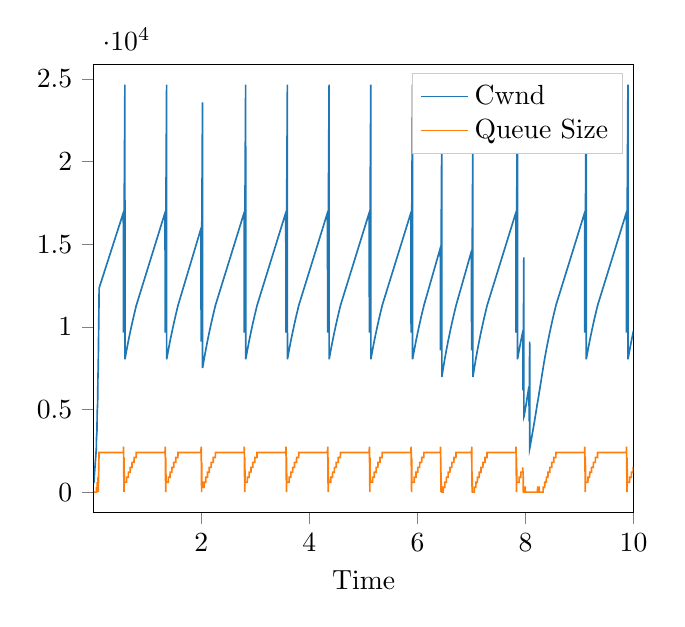
\begin{tikzpicture}

\definecolor{color0}{rgb}{0.12156862745098,0.466666666666667,0.705882352941177}
\definecolor{color1}{rgb}{1,0.498039215686275,0.0549019607843137}

\begin{axis}[
xlabel={Time},
xmin=0.0101856, xmax=9.99934,
ymin=-1232.8, ymax=25888.8,
tick align=outside,
tick pos=left,
x grid style={lightgray!92.026143790849673!black},
y grid style={lightgray!92.026143790849673!black},
legend cell align={left},
legend entries={{Cwnd},{Queue Size}},
legend style={draw=white!80.0!black}
]
\addlegendimage{no markers, color0}
\addlegendimage{no markers, color1}
\addplot [semithick, color0]
table {%
0.0101856 536
0.0213024 1072
0.0332768 1608
0.0452512 2144
0.0562816 2680
0.0581696 3216
0.068256 3752
0.070144 4288
0.072032 4824
0.0802304 5360
0.0821184 5896
0.0840064 6432
0.0858944 6968
0.0912608 7504
0.0931488 8040
0.0950368 8576
0.0969248 9112
0.0988128 9648
0.100701 10184
0.102589 10720
0.104477 11256
0.106365 11792
0.108253 12328
0.108253 12351
0.55382 16879
0.555708 16896
0.55854 9648
0.559484 10184
0.560428 10720
0.561372 11256
0.562316 11792
0.56326 12328
0.564204 12864
0.565148 13400
0.566092 13936
0.567036 14472
0.56798 15008
0.568924 15544
0.569868 16080
0.570812 16616
0.571756 17152
0.5727 17688
0.573644 18224
0.574588 18760
0.575532 19296
0.576476 19832
0.57742 20368
0.578364 20904
0.579308 21440
0.580252 21976
0.581196 22512
0.58214 23048
0.583084 23584
0.584028 24120
0.584972 24656
0.585916 8040
0.587804 8075
0.614236 8552
0.616124 8585
0.618012 8618
0.6199 8651
0.646332 9098
0.64822 9129
0.650108 9160
0.651996 9191
0.680316 9642
0.682204 9671
0.684092 9700
0.68598 9729
0.7143 10156
0.716188 10184
0.718076 10212
0.719964 10240
0.75206 10698
0.753948 10724
0.755836 10750
0.757724 10776
0.791708 11237
0.793596 11262
0.795484 11287
0.797372 11312
1.32601 16885
1.3279 16902
1.33073 9648
1.33168 10184
1.33262 10720
1.33356 11256
1.33451 11792
1.33545 12328
1.3364 12864
1.33734 13400
1.33828 13936
1.33923 14472
1.34017 15008
1.34112 15544
1.34206 16080
1.343 16616
1.34395 17152
1.34489 17688
1.34584 18224
1.34678 18760
1.34772 19296
1.34867 19832
1.34961 20368
1.35056 20904
1.3515 21440
1.35244 21976
1.35339 22512
1.35433 23048
1.35528 23584
1.35622 24120
1.35716 24656
1.35811 8040
1.36 8075
1.38643 8552
1.38832 8585
1.3902 8618
1.39209 8651
1.41852 9098
1.42041 9129
1.4223 9160
1.42419 9191
1.45251 9642
1.4544 9671
1.45628 9700
1.45817 9729
1.48649 10156
1.48838 10184
1.49027 10212
1.49216 10240
1.52425 10698
1.52614 10724
1.52803 10750
1.52992 10776
1.5639 11237
1.56579 11262
1.56768 11287
1.56956 11312
1.99059 15913
1.99247 15931
1.99625 9112
1.99719 9648
1.99814 10184
1.99908 10720
2.00003 11256
2.00097 11792
2.00191 12328
2.00286 12864
2.0038 13400
2.00475 13936
2.00569 14472
2.00663 15008
2.00758 15544
2.00852 16080
2.00947 16616
2.01041 17152
2.01135 17688
2.0123 18224
2.01324 18760
2.01419 19296
2.01513 19832
2.01607 20368
2.01702 20904
2.01796 21440
2.01891 21976
2.01985 22512
2.02079 23048
2.02174 23584
2.02268 7504
2.02457 7542
2.02646 7580
2.04911 8016
2.051 8051
2.05289 8086
2.05478 8121
2.07932 8563
2.08121 8596
2.0831 8629
2.08499 8662
2.11142 9108
2.11331 9139
2.11519 9170
2.11708 9201
2.14351 9623
2.1454 9652
2.14729 9681
2.14918 9710
2.17939 10165
2.18127 10193
2.18316 10221
2.18505 10249
2.21715 10707
2.21903 10733
2.22092 10759
2.22281 10785
2.25679 11246
2.25868 11271
2.26057 11296
2.26246 11321
2.78921 16873
2.7911 16890
2.79393 9648
2.79487 10184
2.79582 10720
2.79676 11256
2.79771 11792
2.79865 12328
2.79959 12864
2.80054 13400
2.80148 13936
2.80243 14472
2.80337 15008
2.80431 15544
2.80526 16080
2.8062 16616
2.80715 17152
2.80809 17688
2.80903 18224
2.80998 18760
2.81092 19296
2.81187 19832
2.81281 20368
2.81375 20904
2.8147 21440
2.81564 21976
2.81659 22512
2.81753 23048
2.81847 23584
2.81942 24120
2.82036 24656
2.82131 8040
2.82319 8075
2.84963 8552
2.85151 8585
2.8534 8618
2.85529 8651
2.88172 9098
2.88361 9129
2.8855 9160
2.88739 9191
2.91571 9642
2.91759 9671
2.91948 9700
2.92137 9729
2.94969 10156
2.95158 10184
2.95347 10212
2.95535 10240
2.98745 10698
2.98934 10724
2.99123 10750
2.99311 10776
3.0271 11237
3.02899 11262
3.03087 11287
3.03276 11312
3.5614 16885
3.56329 16902
3.56612 9648
3.56707 10184
3.56801 10720
3.56895 11256
3.5699 11792
3.57084 12328
3.57179 12864
3.57273 13400
3.57367 13936
3.57462 14472
3.57556 15008
3.57651 15544
3.57745 16080
3.57839 16616
3.57934 17152
3.58028 17688
3.58123 18224
3.58217 18760
3.58311 19296
3.58406 19832
3.585 20368
3.58595 20904
3.58689 21440
3.58783 21976
3.58878 22512
3.58972 23048
3.59067 23584
3.59161 24120
3.59255 24656
3.5935 8040
3.59539 8075
3.62182 8552
3.62371 8585
3.62559 8618
3.62748 8651
3.65391 9098
3.6558 9129
3.65769 9160
3.65958 9191
3.6879 9642
3.68978 9671
3.69167 9700
3.69356 9729
3.72188 10156
3.72377 10184
3.72566 10212
3.72754 10240
3.75964 10698
3.76153 10724
3.76342 10750
3.7653 10776
3.79929 11237
3.80118 11262
3.80306 11287
3.80495 11312
4.33359 16885
4.33548 16902
4.33831 9648
4.33926 10184
4.3402 10720
4.34114 11256
4.34209 11792
4.34303 12328
4.34398 12864
4.34492 13400
4.34586 13936
4.34681 14472
4.34775 15008
4.3487 15544
4.34964 16080
4.35058 16616
4.35153 17152
4.35247 17688
4.35342 18224
4.35436 18760
4.3553 19296
4.35625 19832
4.35719 20368
4.35814 20904
4.35908 21440
4.36002 21976
4.36097 22512
4.36191 23048
4.36286 23584
4.3638 24120
4.36474 24656
4.36569 8040
4.36758 8075
4.39401 8552
4.3959 8585
4.39778 8618
4.39967 8651
4.4261 9098
4.42799 9129
4.42988 9160
4.43177 9191
4.46009 9642
4.46198 9671
4.46386 9700
4.46575 9729
4.49407 10156
4.49596 10184
4.49785 10212
4.49974 10240
4.53183 10698
4.53372 10724
4.53561 10750
4.5375 10776
4.57148 11237
4.57337 11262
4.57526 11287
4.57714 11312
5.10578 16885
5.10767 16902
5.1105 9648
5.11145 10184
5.11239 10720
5.11334 11256
5.11428 11792
5.11522 12328
5.11617 12864
5.11711 13400
5.11806 13936
5.119 14472
5.11994 15008
5.12089 15544
5.12183 16080
5.12278 16616
5.12372 17152
5.12466 17688
5.12561 18224
5.12655 18760
5.1275 19296
5.12844 19832
5.12938 20368
5.13033 20904
5.13127 21440
5.13222 21976
5.13316 22512
5.1341 23048
5.13505 23584
5.13599 24120
5.13694 24656
5.13788 8040
5.13977 8075
5.1662 8552
5.16809 8585
5.16998 8618
5.17186 8651
5.1983 9098
5.20018 9129
5.20207 9160
5.20396 9191
5.23228 9642
5.23417 9671
5.23606 9700
5.23794 9729
5.26626 10156
5.26815 10184
5.27004 10212
5.27193 10240
5.30402 10698
5.30591 10724
5.3078 10750
5.30969 10776
5.34367 11237
5.34556 11262
5.34745 11287
5.34934 11312
5.87797 16885
5.87986 16902
5.88269 9648
5.88364 10184
5.88458 10720
5.88553 11256
5.88647 11792
5.88741 12328
5.88836 12864
5.8893 13400
5.89025 13936
5.89119 14472
5.89213 15008
5.89308 15544
5.89402 16080
5.89497 16616
5.89591 17152
5.89685 17688
5.8978 18224
5.89874 18760
5.89969 19296
5.90063 19832
5.90157 20368
5.90252 20904
5.90346 21440
5.90441 21976
5.90535 22512
5.90629 23048
5.90724 23584
5.90818 24120
5.90913 24656
5.91007 8040
5.91196 8075
5.93839 8552
5.94028 8585
5.94217 8618
5.94405 8651
5.97049 9098
5.97237 9129
5.97426 9160
5.97615 9191
6.00447 9642
6.00636 9671
6.00825 9700
6.01013 9729
6.03845 10156
6.04034 10184
6.04223 10212
6.04412 10240
6.07621 10698
6.0781 10724
6.07999 10750
6.08188 10776
6.11586 11237
6.11775 11262
6.11964 11287
6.12153 11312
6.42172 14741
6.42361 14760
6.42738 8576
6.42833 9112
6.42927 9648
6.43021 10184
6.43116 10720
6.4321 11256
6.43305 11792
6.43399 12328
6.43493 12864
6.43588 13400
6.43682 13936
6.43777 14472
6.43871 15008
6.43965 15544
6.4406 16080
6.44154 16616
6.44249 17152
6.44343 17688
6.44437 18224
6.44532 18760
6.44626 19296
6.44721 19832
6.44815 20368
6.44909 20904
6.45004 21440
6.45098 21976
6.45193 6968
6.45381 7009
6.4557 7049
6.47647 7480
6.47836 7518
6.48025 7556
6.48213 7594
6.50479 8030
6.50668 8065
6.50857 8100
6.51045 8135
6.53311 8544
6.535 8577
6.53689 8610
6.53877 8643
6.56521 9090
6.56709 9121
6.56898 9152
6.57087 9183
6.59919 9635
6.60108 9664
6.60297 9693
6.60485 9722
6.63506 10177
6.63695 10205
6.63884 10233
6.64073 10261
6.67282 10718
6.67471 10744
6.6766 10770
6.67849 10796
6.71058 11231
6.71247 11256
6.71436 11281
6.71625 11306
6.99567 14526
6.99756 14545
7.00039 14564
7.00322 8576
7.00417 9112
7.00511 9648
7.00605 10184
7.007 10720
7.00794 11256
7.00889 11792
7.00983 12328
7.01077 12864
7.01172 13400
7.01266 13936
7.01361 14472
7.01455 15008
7.01549 15544
7.01644 16080
7.01738 16616
7.01833 17152
7.01927 17688
7.02021 18224
7.02116 18760
7.0221 19296
7.02305 19832
7.02399 20368
7.02493 20904
7.02588 21440
7.02682 6968
7.02871 7009
7.05137 7480
7.05325 7518
7.05514 7556
7.05703 7594
7.07969 8030
7.08157 8065
7.08346 8100
7.08535 8135
7.10801 8544
7.10989 8577
7.11178 8610
7.11367 8643
7.1401 9090
7.14199 9121
7.14388 9152
7.14577 9183
7.17409 9635
7.17597 9664
7.17786 9693
7.17975 9722
7.20996 10177
7.21185 10205
7.21373 10233
7.21562 10261
7.24772 10718
7.24961 10744
7.25149 10770
7.25338 10796
7.28548 11231
7.28737 11256
7.28925 11281
7.29114 11306
7.81978 16880
7.82167 16897
7.8245 9648
7.82544 10184
7.82639 10720
7.82733 11256
7.82828 11792
7.82922 12328
7.83016 12864
7.83111 13400
7.83205 13936
7.833 14472
7.83394 15008
7.83488 15544
7.83583 16080
7.83677 16616
7.83772 17152
7.83866 17688
7.8396 18224
7.84055 18760
7.84149 19296
7.84244 19832
7.84338 20368
7.84432 20904
7.84527 21440
7.84621 21976
7.84716 22512
7.8481 23048
7.84904 23584
7.84999 24120
7.85093 24656
7.85188 8040
7.85376 8075
7.8802 8552
7.88208 8585
7.88397 8618
7.88586 8651
7.91229 9098
7.91418 9129
7.91607 9160
7.91796 9191
7.94628 9642
7.95005 9700
7.95288 9729
7.95572 6164
7.95666 6700
7.9576 7236
7.95855 7772
7.95949 8308
7.96044 8844
7.96138 9380
7.96232 9916
7.96327 10452
7.96421 10988
7.96516 11524
7.9661 12060
7.96704 12596
7.96799 13132
7.96893 13668
7.96988 14204
7.97082 4556
7.97713 4619
7.98279 4802
7.98911 4861
7.99099 4920
7.99477 5035
8.00108 5092
8.00297 5148
8.01211 5312
8.014 5366
8.02314 5524
8.02503 5576
8.03889 5876
8.04898 6067
8.0619 6342
8.06378 6387
8.06915 4288
8.07104 5360
8.07198 5896
8.07293 6432
8.07387 6968
8.07481 7504
8.07576 8040
8.0767 8576
8.07765 9112
8.08018 2680
8.08679 2787
8.16589 4263
8.17881 4525
8.19078 4771
8.20276 5006
8.21756 5338
8.22293 5391
8.22482 5444
8.22859 5548
8.23396 5599
8.23585 5650
8.24593 5848
8.24782 5897
8.24971 5945
8.25349 6040
8.25791 6087
8.2598 6134
8.27271 6407
8.28186 6582
8.32469 7474
8.32657 7512
8.32846 7550
8.33035 7588
8.35301 8024
8.35489 8059
8.35678 8094
8.35867 8129
8.38321 8571
8.3851 8604
8.38699 8637
8.38888 8670
8.41342 9085
8.41531 9116
8.4172 9147
8.41909 9178
8.44741 9630
8.44929 9659
8.45118 9688
8.45307 9717
8.48328 10172
8.48517 10200
8.48705 10228
8.48894 10256
8.52104 10714
8.52293 10740
8.52481 10766
8.5267 10792
8.56069 11252
8.56257 11277
8.56446 11302
8.56635 11327
9.0931 16878
9.09499 16895
9.09782 9648
9.09877 10184
9.09971 10720
9.10065 11256
9.1016 11792
9.10254 12328
9.10349 12864
9.10443 13400
9.10537 13936
9.10632 14472
9.10726 15008
9.10821 15544
9.10915 16080
9.11009 16616
9.11104 17152
9.11198 17688
9.11293 18224
9.11387 18760
9.11481 19296
9.11576 19832
9.1167 20368
9.11765 20904
9.11859 21440
9.11953 21976
9.12048 22512
9.12142 23048
9.12237 23584
9.12331 24120
9.12425 24656
9.1252 8040
9.12709 8075
9.15352 8552
9.15541 8585
9.15729 8618
9.15918 8651
9.18561 9098
9.1875 9129
9.18939 9160
9.19128 9191
9.2196 9642
9.22149 9671
9.22337 9700
9.22526 9729
9.25358 10156
9.25547 10184
9.25736 10212
9.25924 10240
9.29134 10698
9.29323 10724
9.29512 10750
9.297 10776
9.33099 11237
9.33288 11262
9.33476 11287
9.33665 11312
9.86529 16885
9.86718 16902
9.87001 9648
9.87096 10184
9.8719 10720
9.87284 11256
9.87379 11792
9.87473 12328
9.87568 12864
9.87662 13400
9.87756 13936
9.87851 14472
9.87945 15008
9.8804 15544
9.88134 16080
9.88228 16616
9.88323 17152
9.88417 17688
9.88512 18224
9.88606 18760
9.887 19296
9.88795 19832
9.88889 20368
9.88984 20904
9.89078 21440
9.89172 21976
9.89267 22512
9.89361 23048
9.89456 23584
9.8955 24120
9.89644 24656
9.89739 8040
9.89928 8075
9.92571 8552
9.9276 8585
9.92948 8618
9.93137 8651
9.9578 9098
9.95969 9129
9.96158 9160
9.96347 9191
9.98235 9494
9.98424 9524
9.98612 9554
9.98801 9584
9.9899 9613
9.99179 9642
9.99368 9671
9.99556 9700
9.99745 9729
9.99934 9758
};
\addplot [semithick, color1]
table {%
0.0101856 0
0.0213024 0
0.0332768 0
0.0452512 0
0.0562816 0
0.0581696 300
0.068256 0
0.070144 300
0.072032 600
0.0802304 0
0.0821184 300
0.0840064 600
0.0858944 900
0.0912608 0
0.0931488 300
0.0950368 600
0.0969248 900
0.0988128 1200
0.100701 1500
0.102589 1800
0.104477 2100
0.106365 2400
0.108253 2400
0.108253 2400
0.55382 2400
0.555708 2400
0.55854 2700
0.559484 2700
0.560428 2400
0.561372 2100
0.562316 1800
0.56326 1500
0.564204 1200
0.565148 900
0.566092 600
0.567036 300
0.56798 0
0.568924 2100
0.569868 1800
0.570812 1500
0.571756 1200
0.5727 900
0.573644 600
0.574588 600
0.575532 600
0.576476 600
0.57742 600
0.578364 600
0.579308 600
0.580252 600
0.581196 600
0.58214 600
0.583084 600
0.584028 600
0.584972 600
0.585916 600
0.587804 600
0.614236 600
0.616124 600
0.618012 900
0.6199 900
0.646332 900
0.64822 900
0.650108 1200
0.651996 1200
0.680316 1200
0.682204 1200
0.684092 1500
0.68598 1500
0.7143 1500
0.716188 1500
0.718076 1800
0.719964 1800
0.75206 1800
0.753948 1800
0.755836 2100
0.757724 2100
0.791708 2100
0.793596 2100
0.795484 2400
0.797372 2400
1.32601 2400
1.3279 2400
1.33073 2700
1.33168 2700
1.33262 2400
1.33356 2100
1.33451 1800
1.33545 1500
1.3364 1200
1.33734 900
1.33828 600
1.33923 300
1.34017 0
1.34112 2100
1.34206 1800
1.343 1500
1.34395 1200
1.34489 900
1.34584 600
1.34678 600
1.34772 600
1.34867 600
1.34961 600
1.35056 600
1.3515 600
1.35244 600
1.35339 600
1.35433 600
1.35528 600
1.35622 600
1.35716 600
1.35811 600
1.36 600
1.38643 600
1.38832 600
1.3902 900
1.39209 900
1.41852 900
1.42041 900
1.4223 1200
1.42419 1200
1.45251 1200
1.4544 1200
1.45628 1500
1.45817 1500
1.48649 1500
1.48838 1500
1.49027 1800
1.49216 1800
1.52425 1800
1.52614 1800
1.52803 2100
1.52992 2100
1.5639 2100
1.56579 2100
1.56768 2400
1.56956 2400
1.99059 2400
1.99247 2400
1.99625 2700
1.99719 2700
1.99814 2400
1.99908 2100
2.00003 1800
2.00097 1500
2.00191 1200
2.00286 900
2.0038 600
2.00475 300
2.00569 0
2.00663 1800
2.00758 1500
2.00852 1200
2.00947 900
2.01041 600
2.01135 600
2.0123 600
2.01324 600
2.01419 600
2.01513 600
2.01607 600
2.01702 600
2.01796 600
2.01891 600
2.01985 600
2.02079 600
2.02174 600
2.02268 600
2.02457 300
2.02646 300
2.04911 300
2.051 300
2.05289 600
2.05478 600
2.07932 600
2.08121 600
2.0831 900
2.08499 900
2.11142 900
2.11331 900
2.11519 1200
2.11708 1200
2.14351 1200
2.1454 1200
2.14729 1500
2.14918 1500
2.17939 1500
2.18127 1500
2.18316 1800
2.18505 1800
2.21715 1800
2.21903 1800
2.22092 2100
2.22281 2100
2.25679 2100
2.25868 2100
2.26057 2400
2.26246 2400
2.78921 2400
2.7911 2400
2.79393 2700
2.79487 2700
2.79582 2400
2.79676 2100
2.79771 1800
2.79865 1500
2.79959 1200
2.80054 900
2.80148 600
2.80243 300
2.80337 0
2.80431 2100
2.80526 1800
2.8062 1500
2.80715 1200
2.80809 900
2.80903 600
2.80998 600
2.81092 600
2.81187 600
2.81281 600
2.81375 600
2.8147 600
2.81564 600
2.81659 600
2.81753 600
2.81847 600
2.81942 600
2.82036 600
2.82131 600
2.82319 600
2.84963 600
2.85151 600
2.8534 900
2.85529 900
2.88172 900
2.88361 900
2.8855 1200
2.88739 1200
2.91571 1200
2.91759 1200
2.91948 1500
2.92137 1500
2.94969 1500
2.95158 1500
2.95347 1800
2.95535 1800
2.98745 1800
2.98934 1800
2.99123 2100
2.99311 2100
3.0271 2100
3.02899 2100
3.03087 2400
3.03276 2400
3.5614 2400
3.56329 2400
3.56612 2700
3.56707 2700
3.56801 2400
3.56895 2100
3.5699 1800
3.57084 1500
3.57179 1200
3.57273 900
3.57367 600
3.57462 300
3.57556 0
3.57651 2100
3.57745 1800
3.57839 1500
3.57934 1200
3.58028 900
3.58123 600
3.58217 600
3.58311 600
3.58406 600
3.585 600
3.58595 600
3.58689 600
3.58783 600
3.58878 600
3.58972 600
3.59067 600
3.59161 600
3.59255 600
3.5935 600
3.59539 600
3.62182 600
3.62371 600
3.62559 900
3.62748 900
3.65391 900
3.6558 900
3.65769 1200
3.65958 1200
3.6879 1200
3.68978 1200
3.69167 1500
3.69356 1500
3.72188 1500
3.72377 1500
3.72566 1800
3.72754 1800
3.75964 1800
3.76153 1800
3.76342 2100
3.7653 2100
3.79929 2100
3.80118 2100
3.80306 2400
3.80495 2400
4.33359 2400
4.33548 2400
4.33831 2700
4.33926 2700
4.3402 2400
4.34114 2100
4.34209 1800
4.34303 1500
4.34398 1200
4.34492 900
4.34586 600
4.34681 300
4.34775 0
4.3487 2100
4.34964 1800
4.35058 1500
4.35153 1200
4.35247 900
4.35342 600
4.35436 600
4.3553 600
4.35625 600
4.35719 600
4.35814 600
4.35908 600
4.36002 600
4.36097 600
4.36191 600
4.36286 600
4.3638 600
4.36474 600
4.36569 600
4.36758 600
4.39401 600
4.3959 600
4.39778 900
4.39967 900
4.4261 900
4.42799 900
4.42988 1200
4.43177 1200
4.46009 1200
4.46198 1200
4.46386 1500
4.46575 1500
4.49407 1500
4.49596 1500
4.49785 1800
4.49974 1800
4.53183 1800
4.53372 1800
4.53561 2100
4.5375 2100
4.57148 2100
4.57337 2100
4.57526 2400
4.57714 2400
5.10578 2400
5.10767 2400
5.1105 2700
5.11145 2700
5.11239 2400
5.11334 2100
5.11428 1800
5.11522 1500
5.11617 1200
5.11711 900
5.11806 600
5.119 300
5.11994 0
5.12089 2100
5.12183 1800
5.12278 1500
5.12372 1200
5.12466 900
5.12561 600
5.12655 600
5.1275 600
5.12844 600
5.12938 600
5.13033 600
5.13127 600
5.13222 600
5.13316 600
5.1341 600
5.13505 600
5.13599 600
5.13694 600
5.13788 600
5.13977 600
5.1662 600
5.16809 600
5.16998 900
5.17186 900
5.1983 900
5.20018 900
5.20207 1200
5.20396 1200
5.23228 1200
5.23417 1200
5.23606 1500
5.23794 1500
5.26626 1500
5.26815 1500
5.27004 1800
5.27193 1800
5.30402 1800
5.30591 1800
5.3078 2100
5.30969 2100
5.34367 2100
5.34556 2100
5.34745 2400
5.34934 2400
5.87797 2400
5.87986 2400
5.88269 2700
5.88364 2700
5.88458 2400
5.88553 2100
5.88647 1800
5.88741 1500
5.88836 1200
5.8893 900
5.89025 600
5.89119 300
5.89213 0
5.89308 2100
5.89402 1800
5.89497 1500
5.89591 1200
5.89685 900
5.8978 600
5.89874 600
5.89969 600
5.90063 600
5.90157 600
5.90252 600
5.90346 600
5.90441 600
5.90535 600
5.90629 600
5.90724 600
5.90818 600
5.90913 600
5.91007 600
5.91196 600
5.93839 600
5.94028 600
5.94217 900
5.94405 900
5.97049 900
5.97237 900
5.97426 1200
5.97615 1200
6.00447 1200
6.00636 1200
6.00825 1500
6.01013 1500
6.03845 1500
6.04034 1500
6.04223 1800
6.04412 1800
6.07621 1800
6.0781 1800
6.07999 2100
6.08188 2100
6.11586 2100
6.11775 2100
6.11964 2400
6.12153 2400
6.42172 2400
6.42361 2400
6.42738 2700
6.42833 2700
6.42927 2400
6.43021 2100
6.43116 1800
6.4321 1500
6.43305 1200
6.43399 900
6.43493 600
6.43588 300
6.43682 0
6.43777 1200
6.43871 900
6.43965 600
6.4406 300
6.44154 300
6.44249 300
6.44343 300
6.44437 300
6.44532 300
6.44626 300
6.44721 300
6.44815 300
6.44909 300
6.45004 300
6.45098 300
6.45193 300
6.45381 0
6.4557 0
6.47647 0
6.47836 0
6.48025 300
6.48213 300
6.50479 300
6.50668 300
6.50857 600
6.51045 600
6.53311 600
6.535 600
6.53689 900
6.53877 900
6.56521 900
6.56709 900
6.56898 1200
6.57087 1200
6.59919 1200
6.60108 1200
6.60297 1500
6.60485 1500
6.63506 1500
6.63695 1500
6.63884 1800
6.64073 1800
6.67282 1800
6.67471 1800
6.6766 2100
6.67849 2100
6.71058 2100
6.71247 2100
6.71436 2400
6.71625 2400
6.99567 2400
6.99756 2400
7.00039 2100
7.00322 2700
7.00417 2700
7.00511 2400
7.00605 2100
7.007 1800
7.00794 1500
7.00889 1200
7.00983 900
7.01077 600
7.01172 300
7.01266 0
7.01361 900
7.01455 600
7.01549 300
7.01644 0
7.01738 0
7.01833 0
7.01927 0
7.02021 0
7.02116 0
7.0221 0
7.02305 0
7.02399 0
7.02493 0
7.02588 0
7.02682 0
7.02871 0
7.05137 0
7.05325 0
7.05514 300
7.05703 300
7.07969 300
7.08157 300
7.08346 600
7.08535 600
7.10801 600
7.10989 600
7.11178 900
7.11367 900
7.1401 900
7.14199 900
7.14388 1200
7.14577 1200
7.17409 1200
7.17597 1200
7.17786 1500
7.17975 1500
7.20996 1500
7.21185 1500
7.21373 1800
7.21562 1800
7.24772 1800
7.24961 1800
7.25149 2100
7.25338 2100
7.28548 2100
7.28737 2100
7.28925 2400
7.29114 2400
7.81978 2400
7.82167 2400
7.8245 2700
7.82544 2700
7.82639 2400
7.82733 2100
7.82828 1800
7.82922 1500
7.83016 1200
7.83111 900
7.83205 600
7.833 300
7.83394 0
7.83488 2100
7.83583 1800
7.83677 1500
7.83772 1200
7.83866 900
7.8396 600
7.84055 600
7.84149 600
7.84244 600
7.84338 600
7.84432 600
7.84527 600
7.84621 600
7.84716 600
7.8481 600
7.84904 600
7.84999 600
7.85093 600
7.85188 600
7.85376 600
7.8802 600
7.88208 600
7.88397 900
7.88586 900
7.91229 900
7.91418 900
7.91607 1200
7.91796 1200
7.94628 1200
7.95005 1500
7.95288 1200
7.95572 1200
7.95666 1200
7.9576 900
7.95855 600
7.95949 300
7.96044 0
7.96138 0
7.96232 0
7.96327 0
7.96421 0
7.96516 0
7.9661 0
7.96704 0
7.96799 0
7.96893 0
7.96988 0
7.97082 0
7.97713 0
7.98279 0
7.98911 0
7.99099 300
7.99477 300
8.00108 0
8.00297 0
8.01211 0
8.014 0
8.02314 0
8.02503 0
8.03889 0
8.04898 0
8.0619 0
8.06378 0
8.06915 0
8.07104 0
8.07198 0
8.07293 0
8.07387 0
8.07481 0
8.07576 0
8.0767 0
8.07765 0
8.08018 0
8.08679 0
8.16589 0
8.17881 0
8.19078 0
8.20276 0
8.21756 0
8.22293 0
8.22482 300
8.22859 300
8.23396 0
8.23585 0
8.24593 0
8.24782 0
8.24971 300
8.25349 300
8.25791 0
8.2598 0
8.27271 0
8.28186 0
8.32469 0
8.32657 0
8.32846 300
8.33035 300
8.35301 300
8.35489 300
8.35678 600
8.35867 600
8.38321 600
8.3851 600
8.38699 900
8.38888 900
8.41342 900
8.41531 900
8.4172 1200
8.41909 1200
8.44741 1200
8.44929 1200
8.45118 1500
8.45307 1500
8.48328 1500
8.48517 1500
8.48705 1800
8.48894 1800
8.52104 1800
8.52293 1800
8.52481 2100
8.5267 2100
8.56069 2100
8.56257 2100
8.56446 2400
8.56635 2400
9.0931 2400
9.09499 2400
9.09782 2700
9.09877 2700
9.09971 2400
9.10065 2100
9.1016 1800
9.10254 1500
9.10349 1200
9.10443 900
9.10537 600
9.10632 300
9.10726 0
9.10821 2100
9.10915 1800
9.11009 1500
9.11104 1200
9.11198 900
9.11293 600
9.11387 600
9.11481 600
9.11576 600
9.1167 600
9.11765 600
9.11859 600
9.11953 600
9.12048 600
9.12142 600
9.12237 600
9.12331 600
9.12425 600
9.1252 600
9.12709 600
9.15352 600
9.15541 600
9.15729 900
9.15918 900
9.18561 900
9.1875 900
9.18939 1200
9.19128 1200
9.2196 1200
9.22149 1200
9.22337 1500
9.22526 1500
9.25358 1500
9.25547 1500
9.25736 1800
9.25924 1800
9.29134 1800
9.29323 1800
9.29512 2100
9.297 2100
9.33099 2100
9.33288 2100
9.33476 2400
9.33665 2400
9.86529 2400
9.86718 2400
9.87001 2700
9.87096 2700
9.8719 2400
9.87284 2100
9.87379 1800
9.87473 1500
9.87568 1200
9.87662 900
9.87756 600
9.87851 300
9.87945 0
9.8804 2100
9.88134 1800
9.88228 1500
9.88323 1200
9.88417 900
9.88512 600
9.88606 600
9.887 600
9.88795 600
9.88889 600
9.88984 600
9.89078 600
9.89172 600
9.89267 600
9.89361 600
9.89456 600
9.8955 600
9.89644 600
9.89739 600
9.89928 600
9.92571 600
9.9276 600
9.92948 900
9.93137 900
9.9578 900
9.95969 900
9.96158 1200
9.96347 1200
9.98235 1200
9.98424 1200
9.98612 1200
9.98801 1200
9.9899 1200
9.99179 1200
9.99368 1200
9.99556 1500
9.99745 1500
9.99934 1500
};
\end{axis}

\end{tikzpicture}\end{center}
Further, if we plot the sequence number of the ACKs received against time, we observe it to be a straight line. However, if we zoom in to the points where cwnd reduces, we observe the following graph.\\
\begin{center}% This file was created by matplotlib2tikz v0.6.13.
\begin{tikzpicture}

\definecolor{color0}{rgb}{0.12156862745098,0.466666666666667,0.705882352941177}

\begin{axis}[
title={Ack Number},
xlabel={Time},
xmin=1.201403, xmax=1.599771,
ymin=632427.4, ymax=881238.6,
tick align=outside,
tick pos=left,
x grid style={lightgray!92.026143790849673!black},
y grid style={lightgray!92.026143790849673!black},
legend entries={{tcp.ack}},
legend cell align={left},
legend style={at={(0.03,0.97)}, anchor=north west, draw=white!80.0!black}
]
\addlegendimage{no markers, color0}
\addplot [semithick, color0]
table {%
1.201403 643737
1.203291 644809
1.205179 645881
1.207067 646953
1.208955 648025
1.210843 649097
1.212731 650169
1.214619 651241
1.216507 652313
1.218395 653385
1.220283 654457
1.222171 655529
1.224059 656601
1.225947 657673
1.227835 658745
1.229723 659817
1.231611 660889
1.233499 661961
1.235387 663033
1.237275 664105
1.239163 665177
1.241051 666249
1.242939 667321
1.244827 668393
1.246715 669465
1.248603 670537
1.250491 671609
1.252379 672681
1.254267 673753
1.256155 674825
1.258043 675897
1.259931 676969
1.261819 678041
1.263707 679113
1.265595 680185
1.267483 681257
1.269371 682329
1.271259 683401
1.273147 684473
1.275035 685545
1.276923 686617
1.278811 687689
1.280699 688761
1.282587 689833
1.284475 690905
1.286363 691977
1.288251 693049
1.290139 694121
1.292027 695193
1.293915 696265
1.295803 697337
1.297691 698409
1.299579 699481
1.301467 700553
1.303355 701625
1.305243 702697
1.307131 703769
1.309019 704841
1.310907 705913
1.312795 706985
1.314683 708057
1.316571 709129
1.318459 710201
1.320347 711273
1.322235 712345
1.324123 713417
1.326011 714489
1.327899 715025
1.328843 715025
1.329787 715025
1.330731 715025
1.331675 715025
1.332619 715025
1.333563 715025
1.334507 715025
1.335451 715025
1.336395 715025
1.337339 715025
1.338283 715025
1.339227 715025
1.340171 715025
1.341115 715025
1.342059 715025
1.343003 715025
1.343947 715025
1.344891 715025
1.345835 715025
1.346779 715025
1.347723 715025
1.348667 715025
1.349611 715025
1.350555 715025
1.351499 715025
1.352443 715025
1.353387 715025
1.354331 715025
1.355275 715025
1.356219 715025
1.357163 715025
1.358107 732713
1.359995 733785
1.361883 734857
1.363771 735929
1.365659 737001
1.367547 738073
1.369435 739145
1.371323 740217
1.373211 741289
1.375099 742361
1.376987 743433
1.378875 744505
1.380763 745577
1.382651 746649
1.384539 747721
1.386427 748793
1.388315 749865
1.390203 750937
1.392091 752009
1.393979 753081
1.395867 754153
1.397755 755225
1.399643 756297
1.401531 757369
1.403419 758441
1.405307 759513
1.407195 760585
1.409083 761657
1.410971 762729
1.412859 763801
1.414747 764873
1.416635 765945
1.418523 767017
1.420411 768089
1.422299 769161
1.424187 770233
1.426075 771305
1.427963 772377
1.429851 773449
1.431739 774521
1.433627 775593
1.435515 776665
1.437403 777737
1.439291 778809
1.441179 779881
1.443067 780953
1.444955 782025
1.446843 783097
1.448731 784169
1.450619 785241
1.452507 786313
1.454395 787385
1.456283 788457
1.458171 789529
1.460059 790601
1.461947 791673
1.463835 792745
1.465723 793817
1.467611 794889
1.469499 795961
1.471387 797033
1.473275 798105
1.475163 799177
1.477051 800249
1.478939 801321
1.480827 802393
1.482715 803465
1.484603 804537
1.486491 805609
1.488379 806681
1.490267 807753
1.492155 808825
1.494043 809897
1.495931 810969
1.497819 812041
1.499707 813113
1.501595 814185
1.503483 815257
1.505371 816329
1.507259 817401
1.509147 818473
1.511035 819545
1.512923 820617
1.514811 821689
1.516699 822761
1.518587 823833
1.520475 824905
1.522363 825977
1.524251 827049
1.526139 828121
1.528027 829193
1.529915 830265
1.531803 831337
1.533691 832409
1.535579 833481
1.537467 834553
1.539355 835625
1.541243 836697
1.543131 837769
1.545019 838841
1.546907 839913
1.548795 840985
1.550683 842057
1.552571 843129
1.554459 844201
1.556347 845273
1.558235 846345
1.560123 847417
1.562011 848489
1.563899 849561
1.565787 850633
1.567675 851705
1.569563 852777
1.571451 853849
1.573339 854921
1.575227 855993
1.577115 857065
1.579003 858137
1.580891 859209
1.582779 860281
1.584667 861353
1.586555 862425
1.588443 863497
1.590331 864569
1.592219 865641
1.594107 866713
1.595995 867785
1.597883 868857
1.599771 869929
};
\end{axis}

\end{tikzpicture}\end{center}
The following inferences can be drawn from the two figures above:
\begin{itemize}
	\item The size of cwnd increases quadratically at the start after Slow Start. After this, the size increases linearly and reduces periodically. During the time of simulation, it reduces 13 times.
	\item Multiple ACKs with the same sequence number are received before the reduction in cwnd. After cwnd reduces, the sequencce number jumps suddenly to the linearly expected value. This confirms that the size of cwnd reduces after multiple DupACKs are received.
	\item The queue gets filled quickly before the size of cwnd reduces.
\end{itemize}

\item Start with the default config. Change the link bandwidth to 50Mbps (from 5 Mbps).
\begin{itemize}
	\item What is the average throughput of the TCP transfer? What is the maximum expected value of throughput? Is the achieved throughput approximately equal to the maximum expected value? If it is not, explain the reason for the difference. 
	\item What other parameters in the simulation (amongst the ones exposed to you above) can you change to make sure that the throughput is close to the maximum expected value, for this link bandwidth? (Try out a few different simulations, and see what gets you close to the maximum.) 
\end{itemize}

Setting bandwidth to 50 Mbps, we get the following throughputs:
\begin{verbatim}
TCP Receiving Throughput : 14668 kbps
Receiving Throughput : 16145 kbps
\end{verbatim}
Thus, while increasing in absolute terms, the throughput gets much worse when compared to what is expected. Further, it can be observed that on reducing the delay to 1ms, we get,
\begin{verbatim}
TCP Receiving Throughput : 37458 kbps
Receiving Throughput : 41232 kbps
\end{verbatim}
This can be explained by looking at the size of cwnd. At a latency of 5ms, we see the following:
\begin{center}% This file was created by matplotlib2tikz v0.6.13.
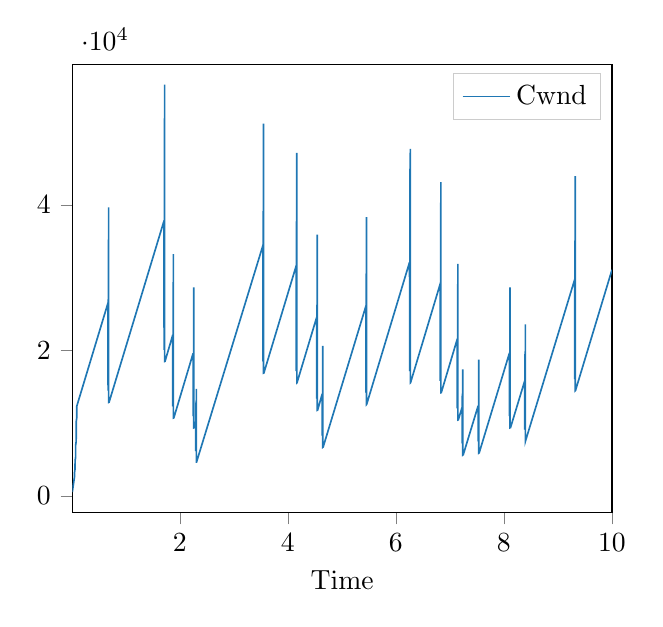
\begin{tikzpicture}

\definecolor{color0}{rgb}{0.12156862745098,0.466666666666667,0.705882352941177}

\begin{axis}[
xlabel={Time},
xmin=0.0100186, xmax=9.99984,
ymin=-2264.6, ymax=59348.6,
tick align=outside,
tick pos=left,
x grid style={lightgray!92.026143790849673!black},
y grid style={lightgray!92.026143790849673!black},
legend cell align={left},
legend entries={{Cwnd}},
legend style={draw=white!80.0!black}
]
\addlegendimage{no markers, color0}
\addplot [semithick, color0]
table {%
0.0100186 536
0.0201302 1072
0.0303277 1608
0.0405251 2144
0.0506282 2680
0.050817 3216
0.0608256 3752
0.0610144 4288
0.0612032 4824
0.071023 5360
0.0712118 5896
0.0714006 6432
0.0715894 6968
0.0811261 7504
0.0813149 8040
0.0815037 8576
0.0816925 9112
0.0818813 9648
0.0820701 10184
0.0912291 10720
0.0914179 11256
0.0916067 11792
0.0917955 12328
0.671445 26556
0.671634 26566
0.672011 14472
0.672106 15008
0.6722 15544
0.672294 16080
0.672389 16616
0.672483 17152
0.672578 17688
0.672672 18224
0.672766 18760
0.672861 19296
0.672955 19832
0.67305 20368
0.673144 20904
0.673238 21440
0.673333 21976
0.673427 22512
0.673522 23048
0.673616 23584
0.67371 24120
0.673805 24656
0.673899 25192
0.673994 25728
0.674088 26264
0.674182 26800
0.679849 27336
0.679943 27872
0.680038 28408
0.680132 28944
0.680226 29480
0.680321 30016
0.680415 30552
0.68051 31088
0.680604 31624
0.680698 32160
0.680793 32696
0.680887 33232
0.680982 33768
0.681076 34304
0.68117 34840
0.681265 35376
0.681359 35912
0.681454 36448
0.681548 36984
0.681642 37520
0.681737 38056
0.681831 38592
0.681926 39128
0.68202 39664
0.682114 12864
0.690141 12886
1.70819 37839
1.70837 37846
1.70875 20100
1.70885 20636
1.70894 21172
1.70904 21708
1.70913 22244
1.70922 22780
1.70932 23316
1.70941 23852
1.70951 24388
1.7096 24924
1.7097 25460
1.70979 25996
1.70988 26532
1.70998 27068
1.71007 27604
1.71017 28140
1.71026 28676
1.71036 29212
1.71045 29748
1.71055 30284
1.71064 30820
1.71073 31356
1.71083 31892
1.71092 32428
1.71102 32964
1.71111 33500
1.71121 34036
1.7113 34572
1.7114 35108
1.71508 35644
1.71517 36180
1.71527 36716
1.71536 37252
1.71546 37788
1.71555 38324
1.71565 38860
1.71574 39396
1.71583 39932
1.71593 40468
1.71602 41004
1.71612 41540
1.71621 42076
1.71631 42612
1.7164 43148
1.71649 43684
1.71659 44220
1.71668 44756
1.71678 45292
1.71687 45828
1.71697 46364
1.71706 46900
1.71716 47436
1.71725 47972
1.71734 48508
1.71744 49044
1.71753 49580
1.71763 50116
1.71772 50652
1.71782 51188
1.71791 51724
1.71801 52260
1.7181 52796
1.71819 53332
1.71829 53868
1.71838 54404
1.71848 54940
1.71857 55476
1.71867 56012
1.71876 56548
1.71885 18492
1.72594 18507
1.87002 22147
1.87021 22159
1.87059 12328
1.87068 12864
1.87078 13400
1.87087 13936
1.87097 14472
1.87106 15008
1.87116 15544
1.87125 16080
1.87134 16616
1.87144 17152
1.87153 17688
1.87163 18224
1.87172 18760
1.87182 19296
1.87824 19832
1.87833 20368
1.87843 20904
1.87852 21440
1.87862 21976
1.87871 22512
1.8788 23048
1.8789 23584
1.87899 24120
1.87909 24656
1.87918 25192
1.87928 25728
1.87937 26264
1.87947 26800
1.87956 27336
1.87965 27872
1.87975 28408
1.87984 28944
1.87994 29480
1.88003 30016
1.88013 30552
1.88022 31088
1.88031 31624
1.88041 32160
1.8805 32696
1.8806 33232
1.88069 10720
1.8891 10746
2.24629 19605
2.24657 19619
2.24686 10988
2.24695 11524
2.24705 12060
2.24714 12596
2.24723 13132
2.24733 13668
2.24742 14204
2.24752 14740
2.24761 15276
2.2545 15812
2.2546 16348
2.25469 16884
2.25479 17420
2.25488 17956
2.25498 18492
2.25507 19028
2.25517 19564
2.25526 20100
2.25535 20636
2.25545 21172
2.25554 21708
2.25564 22244
2.25573 22780
2.25583 23316
2.25592 23852
2.25602 24388
2.25611 24924
2.2562 25460
2.2563 25996
2.25639 26532
2.25649 27068
2.25668 27604
2.25677 28140
2.25686 28676
2.25696 9380
2.26565 9410
2.28736 10105
2.29605 10133
2.29643 6164
2.29652 6700
2.29662 7236
2.29671 7772
2.29681 8308
2.2969 8844
2.29699 9380
2.29709 9916
2.29718 10452
2.29728 10988
2.29737 11524
2.29747 12060
2.29756 12596
2.30615 13132
2.30625 13668
2.30634 14204
2.30644 14740
2.30653 4556
2.30757 4619
3.53759 34413
3.53787 34421
3.53816 18492
3.53825 19028
3.53834 19564
3.53844 20100
3.53853 20636
3.53863 21172
3.53872 21708
3.53882 22244
3.53891 22780
3.539 23316
3.5391 23852
3.53919 24388
3.53929 24924
3.53938 25460
3.53948 25996
3.53957 26532
3.53967 27068
3.53976 27604
3.53985 28140
3.53995 28676
3.54429 29212
3.54439 29748
3.54448 30284
3.54458 30820
3.54467 31356
3.54477 31892
3.54486 32428
3.54495 32964
3.54505 33500
3.54514 34036
3.54524 34572
3.54533 35108
3.54543 35644
3.54552 36180
3.54562 36716
3.54571 37252
3.5458 37788
3.5459 38324
3.54599 38860
3.54609 39396
3.54618 39932
3.54628 40468
3.54637 41004
3.54646 41540
3.54656 42076
3.54665 42612
3.54675 43148
3.54684 43684
3.54694 44220
3.54703 44756
3.54713 45292
3.54722 45828
3.54731 46364
3.54741 46900
3.5475 47436
3.5476 47972
3.54769 48508
3.54779 49044
3.54788 49580
3.54798 50116
3.54807 50652
3.54816 51188
3.54826 16884
3.55572 16901
4.15557 31663
4.15586 31672
4.15614 17152
4.15623 17688
4.15633 18224
4.15642 18760
4.15652 19296
4.15661 19832
4.15671 20368
4.1568 20904
4.1569 21440
4.15699 21976
4.15708 22512
4.15718 23048
4.15727 23584
4.15737 24120
4.15746 24656
4.15756 25192
4.15765 25728
4.15774 26264
4.15784 26800
4.15793 27336
4.15803 27872
4.15812 28408
4.15822 28944
4.15831 29480
4.15841 30016
4.1585 30552
4.15859 31088
4.15869 31624
4.15878 32160
4.15888 32696
4.15897 33232
4.15907 33768
4.15916 34304
4.15926 34840
4.15935 35376
4.15944 35912
4.15954 36448
4.15963 36984
4.15973 37520
4.16454 38056
4.16464 38592
4.16473 39128
4.16483 39664
4.16492 40200
4.16502 40736
4.16511 41272
4.1652 41808
4.1653 42344
4.16539 42880
4.16549 43416
4.16558 43952
4.16568 44488
4.16577 45024
4.16587 45560
4.16596 46096
4.16605 46632
4.16615 47168
4.16624 15544
4.16917 15562
4.53231 24530
4.53458 24541
4.53486 13400
4.53496 13936
4.53505 14472
4.53514 15008
4.53524 15544
4.53533 16080
4.53543 16616
4.53552 17152
4.53562 17688
4.53571 18224
4.53581 18760
4.5359 19296
4.53996 19832
4.54006 20368
4.54015 20904
4.54024 21440
4.54034 21976
4.54043 22512
4.54053 23048
4.54062 23584
4.54072 24120
4.54081 24656
4.54091 25192
4.541 25728
4.54109 26264
4.54119 26800
4.54128 27336
4.54138 27872
4.54147 28408
4.54157 28944
4.54166 29480
4.54175 30016
4.54185 30552
4.54194 31088
4.54204 31624
4.54213 32160
4.54223 32696
4.54232 33232
4.54242 33768
4.54251 34304
4.54468 34840
4.54478 35376
4.54487 35912
4.54496 11792
4.5512 11816
4.634 13973
4.63608 13993
4.63636 8308
4.63646 8844
4.6426 9380
4.64269 9916
4.64279 10452
4.64288 10988
4.64297 11524
4.64307 12060
4.64316 12596
4.64326 13132
4.64335 13668
4.64345 14204
4.64354 14740
4.64363 15276
4.64373 15812
4.64382 16348
4.64392 16884
4.64401 17420
4.64411 17956
4.6442 18492
4.6443 19028
4.64618 19564
4.64628 20100
4.64637 20636
4.64647 6700
4.65393 6742
5.44649 26141
5.44678 26151
5.44706 14204
5.44716 14740
5.44725 15276
5.44734 15812
5.44744 16348
5.44753 16884
5.44763 17420
5.44772 17956
5.44782 18492
5.44791 19028
5.44801 19564
5.4481 20100
5.44819 20636
5.44829 21172
5.44838 21708
5.44848 22244
5.44857 22780
5.44867 23316
5.44876 23852
5.44885 24388
5.44895 24924
5.44904 25460
5.44914 25996
5.44923 26532
5.44933 27068
5.44942 27604
5.44952 28140
5.44961 28676
5.4497 29212
5.4498 29748
5.44989 30284
5.45565 30820
5.45575 31356
5.45584 31892
5.45594 32428
5.45603 32964
5.45613 33500
5.45622 34036
5.45631 34572
5.45641 35108
5.4565 35644
5.4566 36180
5.45669 36716
5.45688 37252
5.45698 37788
5.45707 38324
5.45716 12596
5.45962 12618
6.25266 32121
6.25285 32129
6.25766 17152
6.25776 17688
6.25785 18224
6.25795 18760
6.25804 19296
6.25814 19832
6.25823 20368
6.25833 20904
6.25842 21440
6.25851 21976
6.25861 22512
6.2587 23048
6.2588 23584
6.25889 24120
6.25899 24656
6.25908 25192
6.25918 25728
6.25927 26264
6.25936 26800
6.25946 27336
6.25955 27872
6.25965 28408
6.25974 28944
6.25984 29480
6.25993 30016
6.26002 30552
6.26012 31088
6.26021 31624
6.26031 32160
6.2604 32696
6.2605 33232
6.26059 33768
6.26069 34304
6.26078 34840
6.26087 35376
6.26097 35912
6.26106 36448
6.26116 36984
6.26144 37520
6.26154 38056
6.26163 38592
6.26172 39128
6.26182 39664
6.26191 40200
6.26201 40736
6.2621 41272
6.2622 41808
6.26229 42344
6.26238 42880
6.26248 43416
6.26257 43952
6.26267 44488
6.26276 45024
6.26286 45560
6.26295 46096
6.26305 46632
6.26758 47168
6.26767 47704
6.26777 15544
6.27069 15562
6.82202 29194
6.8223 29203
6.82258 15812
6.82268 16348
6.82277 16884
6.82287 17420
6.82296 17956
6.82306 18492
6.82315 19028
6.82324 19564
6.82334 20100
6.8257 20636
6.82579 21172
6.82872 21708
6.82882 22244
6.82891 22780
6.829 23316
6.8291 23852
6.82919 24388
6.82929 24924
6.82938 25460
6.82948 25996
6.82957 26532
6.82967 27068
6.82976 27604
6.82985 28140
6.82995 28676
6.83004 29212
6.83014 29748
6.83023 30284
6.83033 30820
6.83042 31356
6.83051 31892
6.83061 32428
6.8307 32964
6.8308 33500
6.83089 34036
6.83099 34572
6.83108 35108
6.83118 35644
6.83127 36180
6.83136 36716
6.83146 37252
6.83155 37788
6.83165 38324
6.83174 38860
6.83184 39396
6.83193 39932
6.83203 40468
6.83212 41004
6.83221 41540
6.8324 42076
6.8325 42612
6.83259 43148
6.83269 14204
6.84052 14224
7.13672 21587
7.137 21600
7.13729 12060
7.13738 12596
7.13748 13132
7.13757 13668
7.13767 14204
7.13776 14740
7.13785 15276
7.13795 15812
7.13804 16348
7.13814 16884
7.13823 17420
7.13833 17956
7.13842 18492
7.14494 19028
7.14503 19564
7.14513 20100
7.14522 20636
7.14531 21172
7.14541 21708
7.1455 22244
7.1456 22780
7.14569 23316
7.14579 23852
7.14588 24388
7.14597 24924
7.14607 25460
7.14616 25996
7.14626 26532
7.14635 27068
7.14645 27604
7.14654 28140
7.14664 28676
7.14673 29212
7.14682 29748
7.14692 30284
7.14711 30820
7.1472 31356
7.1473 31892
7.14739 10452
7.15589 10479
7.22708 12217
7.22737 12240
7.22765 7236
7.22774 7772
7.22784 8308
7.22793 8844
7.22803 9380
7.22812 9916
7.22822 10452
7.22831 10988
7.2284 11524
7.2285 12060
7.22859 12596
7.22869 13132
7.22878 13668
7.237 14204
7.23709 14740
7.23719 15276
7.23728 15812
7.23747 16348
7.23756 16884
7.23766 17420
7.23775 5628
7.2471 5679
7.52234 12385
7.52252 12408
7.5229 7504
7.523 8040
7.52309 8576
7.53131 9112
7.5314 9648
7.5315 10184
7.53159 10720
7.53168 11256
7.53178 11792
7.53187 12328
7.53197 12864
7.53206 13400
7.53216 13936
7.53225 14472
7.53234 15008
7.53244 15544
7.53253 16080
7.53263 16616
7.53272 17152
7.53282 17688
7.53291 18224
7.53301 18760
7.5331 5896
7.54235 5944
8.10302 19671
8.10331 19685
8.10359 10988
8.11048 11524
8.11058 12060
8.11067 12596
8.11077 13132
8.11086 13668
8.11096 14204
8.11105 14740
8.11114 15276
8.11124 15812
8.11133 16348
8.11143 16884
8.11152 17420
8.11162 17956
8.11171 18492
8.11181 19028
8.1119 19564
8.11199 20100
8.11209 20636
8.11218 21172
8.11228 21708
8.11237 22244
8.11247 22780
8.11256 23316
8.11265 23852
8.11275 24388
8.11284 24924
8.11294 25460
8.11303 25996
8.11313 26532
8.11322 27068
8.11341 27604
8.1135 28140
8.1136 28676
8.11369 9380
8.12238 9410
8.38638 15861
8.38657 15879
8.38695 9112
8.38704 9648
8.38714 10184
8.38723 10720
8.38732 11256
8.38742 11792
8.38751 12328
8.38761 12864
8.3877 13400
8.3878 13936
8.38789 14472
8.38799 15008
8.38808 15544
8.38817 16080
8.38827 16616
8.38836 17152
8.38846 17688
8.38855 18224
8.38865 18760
8.38874 19296
8.3963 19832
8.39639 20368
8.39648 20904
8.39658 21440
8.39667 21976
8.39677 22512
8.39686 23048
8.39696 23584
8.39705 7504
8.39856 7542
9.31095 29776
9.31123 29785
9.31152 16080
9.31161 16616
9.3117 17152
9.3118 17688
9.31189 18224
9.31199 18760
9.31208 19296
9.31218 19832
9.31227 20368
9.31237 20904
9.31246 21440
9.31255 21976
9.31265 22512
9.31274 23048
9.31284 23584
9.31293 24120
9.31303 24656
9.31312 25192
9.31322 25728
9.31331 26264
9.3134 26800
9.3135 27336
9.31359 27872
9.31369 28408
9.31378 28944
9.31388 29480
9.31397 30016
9.31406 30552
9.31416 31088
9.31425 31624
9.31435 32160
9.31444 32696
9.31454 33232
9.31463 33768
9.31473 34304
9.31482 34840
9.31992 35376
9.32001 35912
9.32011 36448
9.3202 36984
9.3203 37520
9.32039 38056
9.32049 38592
9.32058 39128
9.32068 39664
9.32077 40200
9.32086 40736
9.32096 41272
9.32105 41808
9.32115 42344
9.32134 42880
9.32143 43416
9.32152 43952
9.32162 14472
9.32436 14491
9.99418 30934
9.99437 30943
9.99456 30952
9.99474 30961
9.99493 30970
9.99512 30979
9.99531 30988
9.9955 30997
9.99569 31006
9.99984 31015
};
\end{axis}

\end{tikzpicture}\end{center}
At a latency of 1ms, we get,
\begin{center}% This file was created by matplotlib2tikz v0.6.13.
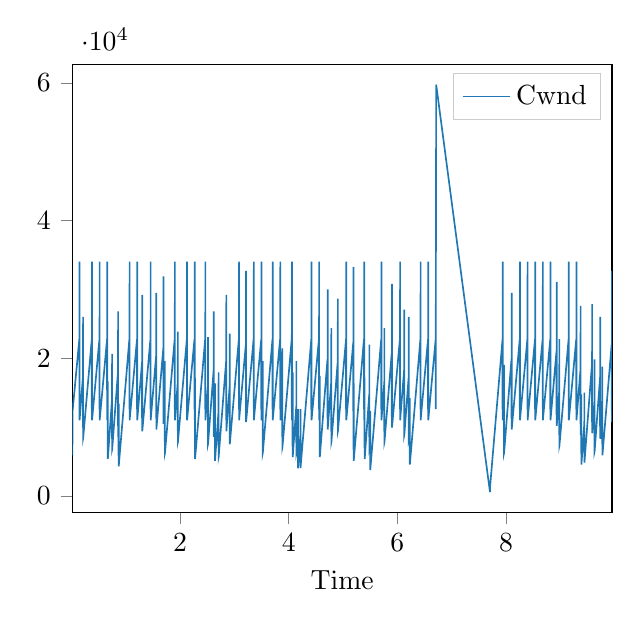
\begin{tikzpicture}

\definecolor{color0}{rgb}{0.12156862745098,0.466666666666667,0.705882352941177}

\begin{axis}[
xlabel={Time},
xmin=0.0152118, xmax=9.95017,
ymin=-2425.4, ymax=62725.4,
tick align=outside,
tick pos=left,
x grid style={lightgray!92.026143790849673!black},
y grid style={lightgray!92.026143790849673!black},
legend cell align={left},
legend entries={{Cwnd}},
legend style={draw=white!80.0!black}
]
\addlegendimage{no markers, color0}
\addplot [semithick, color0]
table {%
0.0152118 5896
0.0154006 6432
0.0155894 6968
0.0171261 7504
0.0173149 8040
0.0175037 8576
0.0176925 9112
0.0178813 9648
0.0180701 10184
0.0192291 10720
0.0194179 11256
0.0196067 11792
0.0197955 12328
0.144293 22760
0.144482 22772
0.144765 12596
0.14486 13132
0.144954 13668
0.145049 14204
0.145143 14740
0.145237 15276
0.145332 15812
0.145426 16348
0.145521 16884
0.145615 17420
0.145709 17956
0.145804 18492
0.145898 19028
0.145993 19564
0.146087 20100
0.146181 20636
0.146276 21172
0.14637 21708
0.146465 22244
0.146559 22780
0.146653 23316
0.146748 23852
0.146842 24388
0.146937 24924
0.147031 25460
0.147125 25996
0.14722 26532
0.147314 27068
0.147409 27604
0.147503 28140
0.147597 28676
0.147692 29212
0.147786 29748
0.147881 30284
0.147975 30820
0.148069 31356
0.148164 31892
0.148258 32428
0.148353 32964
0.148447 33500
0.148541 34036
0.148636 10988
0.14904 11014
0.210043 17272
0.210232 17288
0.21061 9916
0.210704 10452
0.210798 10988
0.210893 11524
0.210987 12060
0.211082 12596
0.211176 13132
0.21127 13668
0.211365 14204
0.211459 14740
0.211554 15276
0.211648 15812
0.211742 16348
0.211837 16884
0.211931 17420
0.212026 17956
0.21212 18492
0.212214 19028
0.212309 19564
0.212403 20100
0.212498 20636
0.212592 21172
0.212686 21708
0.212781 22244
0.212875 22780
0.21297 23316
0.213064 23852
0.213158 24388
0.213253 24924
0.213347 25460
0.213442 25996
0.213536 8308
0.214412 8342
0.373691 22760
0.37388 22772
0.374163 12596
0.374258 13132
0.374352 13668
0.374446 14204
0.374541 14740
0.374635 15276
0.37473 15812
0.374824 16348
0.374918 16884
0.375013 17420
0.375107 17956
0.375202 18492
0.375296 19028
0.37539 19564
0.375485 20100
0.375579 20636
0.375674 21172
0.375768 21708
0.375862 22244
0.375957 22780
0.376051 23316
0.376146 23852
0.37624 24388
0.376334 24924
0.376429 25460
0.376523 25996
0.376618 26532
0.376712 27068
0.376806 27604
0.376901 28140
0.376995 28676
0.37709 29212
0.377184 29748
0.377278 30284
0.377373 30820
0.377467 31356
0.377562 31892
0.377656 32428
0.37775 32964
0.377845 33500
0.377939 34036
0.378034 10988
0.378437 11014
0.514206 22753
0.514395 22765
0.514678 12596
0.514772 13132
0.514867 13668
0.514961 14204
0.515055 14740
0.51515 15276
0.515244 15812
0.515339 16348
0.515433 16884
0.515527 17420
0.515622 17956
0.515716 18492
0.515811 19028
0.515905 19564
0.515999 20100
0.516094 20636
0.516188 21172
0.516283 21708
0.516377 22244
0.516471 22780
0.516566 23316
0.51666 23852
0.516755 24388
0.516849 24924
0.516943 25460
0.517038 25996
0.517132 26532
0.517227 27068
0.517321 27604
0.517415 28140
0.51751 28676
0.517604 29212
0.517699 29748
0.517793 30284
0.517887 30820
0.517982 31356
0.518076 31892
0.518171 32428
0.518265 32964
0.518359 33500
0.518454 34036
0.518548 10988
0.518952 11014
0.65472 22753
0.654909 22765
0.655192 12596
0.655287 13132
0.655381 13668
0.655476 14204
0.65557 14740
0.655664 15276
0.655759 15812
0.655853 16348
0.655948 16884
0.656042 17420
0.656136 17956
0.656231 18492
0.656325 19028
0.65642 19564
0.656514 20100
0.656608 20636
0.656703 21172
0.656797 21708
0.656892 22244
0.656986 22780
0.65708 23316
0.657175 23852
0.657269 24388
0.657364 24924
0.657458 25460
0.657552 25996
0.657647 26532
0.657741 27068
0.657836 27604
0.65793 28140
0.658024 28676
0.658119 29212
0.658213 29748
0.658308 30284
0.658402 30820
0.658496 31356
0.658591 31892
0.658685 32428
0.65878 32964
0.658874 33500
0.658968 34036
0.659063 10988
0.659467 11014
0.665372 11708
0.665655 11732
0.666153 6968
0.666248 7504
0.666342 8040
0.666437 8576
0.666531 9112
0.666625 9648
0.66672 10184
0.666814 10720
0.666909 11256
0.667003 11792
0.667097 12328
0.667192 12864
0.667286 13400
0.667381 13936
0.667475 14472
0.667569 15008
0.667758 15544
0.668068 16080
0.668162 16616
0.668256 5360
0.669389 5413
0.744684 13919
0.744967 13939
0.745251 8308
0.745345 8844
0.745439 9380
0.745534 9916
0.745628 10452
0.745723 10988
0.745817 11524
0.745911 12060
0.746006 12596
0.7461 13132
0.746195 13668
0.746289 14204
0.746383 14740
0.746478 15276
0.746572 15812
0.746667 16348
0.746761 16884
0.746855 17420
0.74695 17956
0.747044 18492
0.747139 19028
0.747233 19564
0.747327 20100
0.747422 20636
0.747516 6700
0.74877 6742
0.854614 17882
0.854802 17898
0.85518 10184
0.855274 10720
0.855369 11256
0.855463 11792
0.855558 12328
0.855652 12864
0.855746 13400
0.855841 13936
0.855935 14472
0.85603 15008
0.856124 15544
0.856218 16080
0.856313 16616
0.856407 17152
0.856502 17688
0.856596 18224
0.85669 18760
0.856785 19296
0.856879 19832
0.856974 20368
0.857068 20904
0.857162 21440
0.857257 21976
0.857351 22512
0.857446 23048
0.85754 23584
0.857634 24120
0.857729 24656
0.857823 25192
0.857918 25728
0.858012 26264
0.858106 26800
0.858201 8576
0.858982 8609
0.865952 9425
0.866235 9455
0.866519 5896
0.866613 6432
0.866707 6968
0.866802 7504
0.866896 8040
0.866991 8576
0.867678 9112
0.867772 9648
0.867866 10184
0.867961 10720
0.868055 11256
0.86815 11792
0.868338 12328
0.868433 12864
0.868527 13400
0.868622 4288
0.870158 4355
1.06566 22762
1.06585 22774
1.06613 12596
1.06623 13132
1.06632 13668
1.06642 14204
1.06651 14740
1.06661 15276
1.0667 15812
1.06679 16348
1.06689 16884
1.06698 17420
1.06708 17956
1.06717 18492
1.06727 19028
1.06736 19564
1.06745 20100
1.06755 20636
1.06764 21172
1.06774 21708
1.06783 22244
1.06793 22780
1.06802 23316
1.06812 23852
1.06821 24388
1.0683 24924
1.0684 25460
1.06849 25996
1.06859 26532
1.06868 27068
1.06878 27604
1.06887 28140
1.06897 28676
1.06906 29212
1.06915 29748
1.06925 30284
1.06934 30820
1.06944 31356
1.06953 31892
1.06963 32428
1.06972 32964
1.06981 33500
1.06991 34036
1.07 10988
1.07041 11014
1.20618 22753
1.20636 22765
1.20665 12596
1.20674 13132
1.20684 13668
1.20693 14204
1.20703 14740
1.20712 15276
1.20721 15812
1.20731 16348
1.2074 16884
1.2075 17420
1.20759 17956
1.20769 18492
1.20778 19028
1.20788 19564
1.20797 20100
1.20806 20636
1.20816 21172
1.20825 21708
1.20835 22244
1.20844 22780
1.20854 23316
1.20863 23852
1.20872 24388
1.20882 24924
1.20891 25460
1.20901 25996
1.2091 26532
1.2092 27068
1.20929 27604
1.20939 28140
1.20948 28676
1.20957 29212
1.20967 29748
1.20976 30284
1.20986 30820
1.20995 31356
1.21005 31892
1.21014 32428
1.21024 32964
1.21033 33500
1.21042 34036
1.21052 10988
1.21092 11014
1.29892 19440
1.29911 19454
1.29949 10988
1.29958 11524
1.29968 12060
1.29977 12596
1.29987 13132
1.29996 13668
1.30006 14204
1.30015 14740
1.30025 15276
1.30034 15812
1.30043 16348
1.30053 16884
1.30062 17420
1.30072 17956
1.30081 18492
1.30091 19028
1.301 19564
1.3011 20100
1.30119 20636
1.30128 21172
1.30138 21708
1.30147 22244
1.30157 22780
1.30166 23316
1.30176 23852
1.30185 24388
1.30194 24924
1.30204 25460
1.30213 25996
1.30223 26532
1.30232 27068
1.30242 27604
1.30251 28140
1.30261 28676
1.3027 29212
1.30279 9380
1.30348 9410
1.45322 22753
1.4534 22765
1.45369 12596
1.45378 13132
1.45388 13668
1.45397 14204
1.45407 14740
1.45416 15276
1.45425 15812
1.45435 16348
1.45444 16884
1.45454 17420
1.45463 17956
1.45473 18492
1.45482 19028
1.45492 19564
1.45501 20100
1.4551 20636
1.4552 21172
1.45529 21708
1.45539 22244
1.45548 22780
1.45558 23316
1.45567 23852
1.45576 24388
1.45586 24924
1.45595 25460
1.45605 25996
1.45614 26532
1.45624 27068
1.45633 27604
1.45643 28140
1.45652 28676
1.45661 29212
1.45671 29748
1.4568 30284
1.4569 30820
1.45699 31356
1.45709 31892
1.45718 32428
1.45728 32964
1.45737 33500
1.45746 34036
1.45756 10988
1.45796 11014
1.55805 20336
1.55833 20350
1.55861 11256
1.55871 11792
1.5588 12328
1.5589 12864
1.55899 13400
1.55909 13936
1.55918 14472
1.55927 15008
1.55937 15544
1.55946 16080
1.55956 16616
1.55965 17152
1.55975 17688
1.55984 18224
1.55994 18760
1.56003 19296
1.56012 19832
1.56022 20368
1.56031 20904
1.56041 21440
1.5605 21976
1.5606 22512
1.56069 23048
1.56078 23584
1.56088 24120
1.56097 24656
1.56107 25192
1.56116 25728
1.56126 26264
1.56135 26800
1.56145 27336
1.56154 27872
1.56163 28408
1.56173 28944
1.56182 29480
1.56192 9648
1.5626 9677
1.69086 21494
1.69114 21507
1.69142 12060
1.69152 12596
1.69161 13132
1.69171 13668
1.6918 14204
1.6919 14740
1.69199 15276
1.69209 15812
1.69218 16348
1.69227 16884
1.69237 17420
1.69246 17956
1.69256 18492
1.69265 19028
1.69275 19564
1.69284 20100
1.69293 20636
1.69303 21172
1.69312 21708
1.69322 22244
1.69331 22780
1.69341 23316
1.6935 23852
1.6936 24388
1.69369 24924
1.69378 25460
1.69388 25996
1.69397 26532
1.69407 27068
1.69416 27604
1.69426 28140
1.69435 28676
1.69445 29212
1.69454 29748
1.69463 30284
1.69473 30820
1.69482 31356
1.69492 31892
1.69501 10452
1.6956 10479
1.7168 12911
1.71701 12933
1.71739 7772
1.71748 8308
1.71758 8844
1.71767 9380
1.71777 9916
1.71786 10452
1.71796 10988
1.71805 11524
1.71814 12060
1.71824 12596
1.71833 13132
1.71843 13668
1.71852 14204
1.71862 14740
1.71871 15276
1.71881 15812
1.7189 16348
1.71899 16884
1.71909 17420
1.71918 17956
1.71928 18492
1.71937 19028
1.71947 19564
1.71956 6164
1.72081 6210
1.89921 22753
1.8994 22765
1.89968 12596
1.89978 13132
1.89987 13668
1.89997 14204
1.90006 14740
1.90015 15276
1.90025 15812
1.90034 16348
1.90044 16884
1.90053 17420
1.90063 17956
1.90072 18492
1.90081 19028
1.90091 19564
1.901 20100
1.9011 20636
1.90119 21172
1.90129 21708
1.90138 22244
1.90148 22780
1.90157 23316
1.90166 23852
1.90176 24388
1.90185 24924
1.90195 25460
1.90204 25996
1.90214 26532
1.90223 27068
1.90233 27604
1.90242 28140
1.90251 28676
1.90261 29212
1.9027 29748
1.9028 30284
1.90289 30820
1.90299 31356
1.90308 31892
1.90317 32428
1.90327 32964
1.90336 33500
1.90346 34036
1.90355 10988
1.90396 11014
1.95514 16411
1.95543 16428
1.95571 9380
1.9558 9916
1.9559 10452
1.95599 10988
1.95609 11524
1.95618 12060
1.95627 12596
1.95637 13132
1.95646 13668
1.95656 14204
1.95665 14740
1.95675 15276
1.95684 15812
1.95694 16348
1.95703 16884
1.95712 17420
1.95722 17956
1.95731 18492
1.95741 19028
1.9575 19564
1.9576 20100
1.95769 20636
1.95779 21172
1.95788 21708
1.95797 22244
1.95807 22780
1.95816 23316
1.95826 23852
1.95835 7772
1.95942 7808
2.12347 22759
2.12366 22771
2.12394 12596
2.12403 13132
2.12413 13668
2.12422 14204
2.12432 14740
2.12441 15276
2.12451 15812
2.1246 16348
2.1247 16884
2.12479 17420
2.12488 17956
2.12498 18492
2.12507 19028
2.12517 19564
2.12526 20100
2.12536 20636
2.12545 21172
2.12554 21708
2.12564 22244
2.12573 22780
2.12583 23316
2.12592 23852
2.12602 24388
2.12611 24924
2.12621 25460
2.1263 25996
2.12639 26532
2.12649 27068
2.12658 27604
2.12668 28140
2.12677 28676
2.12687 29212
2.12696 29748
2.12706 30284
2.12715 30820
2.12724 31356
2.12734 31892
2.12743 32428
2.12753 32964
2.12762 33500
2.12772 34036
2.12781 10988
2.12821 11014
2.26398 22753
2.26417 22765
2.26445 12596
2.26455 13132
2.26464 13668
2.26474 14204
2.26483 14740
2.26493 15276
2.26502 15812
2.26512 16348
2.26521 16884
2.2653 17420
2.2654 17956
2.26549 18492
2.26559 19028
2.26568 19564
2.26578 20100
2.26587 20636
2.26597 21172
2.26606 21708
2.26615 22244
2.26625 22780
2.26634 23316
2.26644 23852
2.26653 24388
2.26663 24924
2.26672 25460
2.26681 25996
2.26691 26532
2.267 27068
2.2671 27604
2.26719 28140
2.26729 28676
2.26738 29212
2.26748 29748
2.26757 30284
2.26766 30820
2.26776 31356
2.26785 31892
2.26795 32428
2.26804 32964
2.26814 33500
2.26823 34036
2.26833 10988
2.26873 11014
2.2713 11316
2.27149 11341
2.27187 6968
2.27196 7504
2.27206 8040
2.27215 8576
2.27225 9112
2.27234 9648
2.27244 10184
2.27253 10720
2.27263 11256
2.27303 11792
2.27312 12328
2.27322 12864
2.27331 13400
2.27341 13936
2.2735 14472
2.2736 15008
2.27369 15544
2.27378 16080
2.27388 16616
2.27397 17152
2.27407 5360
2.27542 5413
2.46097 22763
2.46116 22775
2.46144 12596
2.46154 13132
2.46163 13668
2.46173 14204
2.46182 14740
2.46191 15276
2.46201 15812
2.4621 16348
2.4622 16884
2.46229 17420
2.46239 17956
2.46248 18492
2.46257 19028
2.46267 19564
2.46276 20100
2.46286 20636
2.46295 21172
2.46305 21708
2.46314 22244
2.46324 22780
2.46333 23316
2.46342 23852
2.46352 24388
2.46361 24924
2.46371 25460
2.4638 25996
2.4639 26532
2.46399 27068
2.46409 27604
2.46418 28140
2.46427 28676
2.46437 29212
2.46446 29748
2.46456 30284
2.46465 30820
2.46475 31356
2.46484 31892
2.46493 32428
2.46503 32964
2.46512 33500
2.46522 34036
2.46531 10988
2.46572 11014
2.50973 15753
2.51001 15771
2.51029 9112
2.51039 9648
2.51048 10184
2.51058 10720
2.51067 11256
2.51077 11792
2.51086 12328
2.51095 12864
2.51105 13400
2.51114 13936
2.51124 14472
2.51133 15008
2.51143 15544
2.51152 16080
2.51162 16616
2.51171 17152
2.5118 17688
2.5119 18224
2.51199 18760
2.51209 19296
2.51218 19832
2.51228 20368
2.51237 20904
2.51247 21440
2.51256 21976
2.51265 22512
2.51275 23048
2.51284 7504
2.51391 7542
2.61596 18158
2.61615 18173
2.61653 10184
2.61663 10720
2.61672 11256
2.61681 11792
2.61691 12328
2.617 12864
2.6171 13400
2.61719 13936
2.61729 14472
2.61738 15008
2.61748 15544
2.61757 16080
2.61766 16616
2.61776 17152
2.61785 17688
2.61795 18224
2.61804 18760
2.61814 19296
2.61823 19832
2.61832 20368
2.61842 20904
2.61851 21440
2.61861 21976
2.6187 22512
2.6188 23048
2.61889 23584
2.61899 24120
2.61908 24656
2.61917 25192
2.61927 25728
2.61936 26264
2.61946 26800
2.61955 8576
2.62033 8609
2.63876 10744
2.63895 10770
2.63973 6700
2.63983 7236
2.63992 7772
2.64002 8308
2.64011 8844
2.6402 9380
2.6403 9916
2.64039 10452
2.64049 10988
2.64058 11524
2.64068 12060
2.64077 12596
2.64087 13132
2.64096 13668
2.64105 14204
2.64115 14740
2.64124 15276
2.64134 15812
2.64143 16348
2.64184 5092
2.64297 5148
2.70556 12178
2.70575 12201
2.70613 7236
2.70622 7772
2.70632 8308
2.70641 8844
2.70651 9380
2.7066 9916
2.70669 10452
2.70679 10988
2.70688 11524
2.70698 12060
2.70707 12596
2.70729 13132
2.70738 13668
2.70748 14204
2.70757 14740
2.70766 15276
2.70776 15812
2.70785 16348
2.70795 16884
2.70804 17420
2.70814 17956
2.70823 5628
2.70958 5679
2.84696 19593
2.84715 19607
2.84753 10988
2.84762 11524
2.84772 12060
2.84781 12596
2.84791 13132
2.848 13668
2.8481 14204
2.84819 14740
2.84828 15276
2.84838 15812
2.84847 16348
2.84857 16884
2.84866 17420
2.84876 17956
2.84885 18492
2.84895 19028
2.84904 19564
2.84913 20100
2.84923 20636
2.84932 21172
2.84942 21708
2.84951 22244
2.84961 22780
2.8497 23316
2.84979 23852
2.84989 24388
2.84998 24924
2.85008 25460
2.85017 25996
2.85027 26532
2.85036 27068
2.85046 27604
2.85055 28140
2.85064 28676
2.85074 29212
2.85083 9380
2.85152 9410
2.91063 15861
2.91082 15879
2.9112 9112
2.91129 9648
2.91139 10184
2.91148 10720
2.91157 11256
2.91167 11792
2.91176 12328
2.91186 12864
2.91195 13400
2.91205 13936
2.91214 14472
2.91224 15008
2.91233 15544
2.91242 16080
2.91252 16616
2.91261 17152
2.91271 17688
2.9128 18224
2.9129 18760
2.91299 19296
2.91309 19832
2.91318 20368
2.91327 20904
2.91337 21440
2.91346 21976
2.91356 22512
2.91365 23048
2.91375 23584
2.91384 7504
2.91481 7542
3.08106 22756
3.08125 22768
3.08153 12596
3.08163 13132
3.08172 13668
3.08182 14204
3.08191 14740
3.082 15276
3.0821 15812
3.08219 16348
3.08229 16884
3.08238 17420
3.08248 17956
3.08257 18492
3.08266 19028
3.08276 19564
3.08285 20100
3.08295 20636
3.08304 21172
3.08314 21708
3.08323 22244
3.08333 22780
3.08342 23316
3.08351 23852
3.08361 24388
3.0837 24924
3.0838 25460
3.08389 25996
3.08399 26532
3.08408 27068
3.08418 27604
3.08427 28140
3.08436 28676
3.08446 29212
3.08455 29748
3.08465 30284
3.08474 30820
3.08484 31356
3.08493 31892
3.08502 32428
3.08512 32964
3.08521 33500
3.08531 34036
3.0854 10988
3.08581 11014
3.20987 22001
3.21015 22014
3.21044 12328
3.21053 12864
3.21062 13400
3.21072 13936
3.21081 14472
3.21091 15008
3.211 15544
3.2111 16080
3.21119 16616
3.21128 17152
3.21138 17688
3.21147 18224
3.21157 18760
3.21166 19296
3.21176 19832
3.21185 20368
3.21195 20904
3.21204 21440
3.21213 21976
3.21223 22512
3.21232 23048
3.21242 23584
3.21251 24120
3.21261 24656
3.2127 25192
3.2128 25728
3.21289 26264
3.21298 26800
3.21308 27336
3.21317 27872
3.21327 28408
3.21336 28944
3.21346 29480
3.21355 30016
3.21364 30552
3.21374 31088
3.21383 31624
3.21393 32160
3.21402 32696
3.21412 10720
3.21462 10746
3.35277 22762
3.35296 22774
3.35324 12596
3.35334 13132
3.35343 13668
3.35352 14204
3.35362 14740
3.35371 15276
3.35381 15812
3.3539 16348
3.354 16884
3.35409 17420
3.35419 17956
3.35428 18492
3.35437 19028
3.35447 19564
3.35456 20100
3.35466 20636
3.35475 21172
3.35485 21708
3.35494 22244
3.35504 22780
3.35513 23316
3.35522 23852
3.35532 24388
3.35541 24924
3.35551 25460
3.3556 25996
3.3557 26532
3.35579 27068
3.35588 27604
3.35598 28140
3.35607 28676
3.35617 29212
3.35626 29748
3.35636 30284
3.35645 30820
3.35655 31356
3.35664 31892
3.35673 32428
3.35683 32964
3.35692 33500
3.35702 34036
3.35711 10988
3.35752 11014
3.49328 22753
3.49347 22765
3.49376 12596
3.49385 13132
3.49395 13668
3.49404 14204
3.49413 14740
3.49423 15276
3.49432 15812
3.49442 16348
3.49451 16884
3.49461 17420
3.4947 17956
3.49479 18492
3.49489 19028
3.49498 19564
3.49508 20100
3.49517 20636
3.49527 21172
3.49536 21708
3.49546 22244
3.49555 22780
3.49564 23316
3.49574 23852
3.49583 24388
3.49593 24924
3.49602 25460
3.49612 25996
3.49621 26532
3.49631 27068
3.4964 27604
3.49649 28140
3.49659 28676
3.49668 29212
3.49678 29748
3.49687 30284
3.49697 30820
3.49706 31356
3.49715 31892
3.49725 32428
3.49734 32964
3.49744 33500
3.49753 34036
3.49763 10988
3.49803 11014
3.51769 13262
3.51788 13283
3.51825 7772
3.51835 8308
3.51844 8844
3.51854 9380
3.51863 9916
3.51873 10452
3.51882 10988
3.51891 11524
3.51901 12060
3.5191 12596
3.5192 13132
3.51929 13668
3.51939 14204
3.51948 14740
3.51957 15276
3.51967 15812
3.51976 16348
3.51986 16884
3.51995 17420
3.52005 17956
3.52014 18492
3.52024 19028
3.52033 19564
3.52042 6164
3.52168 6210
3.70007 22753
3.70026 22765
3.70055 12596
3.70064 13132
3.70073 13668
3.70083 14204
3.70092 14740
3.70102 15276
3.70111 15812
3.70121 16348
3.7013 16884
3.7014 17420
3.70149 17956
3.70158 18492
3.70168 19028
3.70177 19564
3.70187 20100
3.70196 20636
3.70206 21172
3.70215 21708
3.70224 22244
3.70234 22780
3.70243 23316
3.70253 23852
3.70262 24388
3.70272 24924
3.70281 25460
3.70291 25996
3.703 26532
3.70309 27068
3.70319 27604
3.70328 28140
3.70338 28676
3.70347 29212
3.70357 29748
3.70366 30284
3.70376 30820
3.70385 31356
3.70394 31892
3.70404 32428
3.70413 32964
3.70423 33500
3.70432 34036
3.70442 10988
3.70482 11014
3.84059 22753
3.84078 22765
3.84106 12596
3.84115 13132
3.84125 13668
3.84134 14204
3.84144 14740
3.84153 15276
3.84163 15812
3.84172 16348
3.84182 16884
3.84191 17420
3.842 17956
3.8421 18492
3.84219 19028
3.84229 19564
3.84238 20100
3.84248 20636
3.84257 21172
3.84266 21708
3.84276 22244
3.84285 22780
3.84295 23316
3.84304 23852
3.84314 24388
3.84323 24924
3.84333 25460
3.84342 25996
3.84351 26532
3.84361 27068
3.8437 27604
3.8438 28140
3.84389 28676
3.84399 29212
3.84408 29748
3.84418 30284
3.84427 30820
3.84436 31356
3.84446 31892
3.84455 32428
3.84465 32964
3.84474 33500
3.84484 34036
3.84493 10988
3.84533 11014
3.87877 14724
3.87906 14743
3.87934 8576
3.87943 9112
3.87953 9648
3.87962 10184
3.87972 10720
3.87981 11256
3.87991 11792
3.88 12328
3.88009 12864
3.88019 13400
3.88028 13936
3.88038 14472
3.88047 15008
3.88057 15544
3.88066 16080
3.88076 16616
3.88085 17152
3.88094 17688
3.88104 18224
3.88113 18760
3.88123 19296
3.88132 19832
3.88142 20368
3.88151 20904
3.88161 21440
3.8817 6968
3.88286 7009
4.054 22760
4.05419 22772
4.05447 12596
4.05457 13132
4.05466 13668
4.05476 14204
4.05485 14740
4.05494 15276
4.05504 15812
4.05513 16348
4.05523 16884
4.05532 17420
4.05542 17956
4.05551 18492
4.05561 19028
4.0557 19564
4.05579 20100
4.05589 20636
4.05598 21172
4.05608 21708
4.05617 22244
4.05627 22780
4.05636 23316
4.05646 23852
4.05655 24388
4.05664 24924
4.05674 25460
4.05683 25996
4.05693 26532
4.05702 27068
4.05712 27604
4.05721 28140
4.0573 28676
4.0574 29212
4.05749 29748
4.05759 30284
4.05768 30820
4.05778 31356
4.05787 31892
4.05797 32428
4.05806 32964
4.05815 33500
4.05825 34036
4.05834 10988
4.05875 11014
4.06955 12248
4.06973 12271
4.07011 7236
4.07021 7772
4.0703 8308
4.0704 8844
4.07049 9380
4.07058 9916
4.07068 10452
4.07077 10988
4.07087 11524
4.07096 12060
4.07106 12596
4.07115 13132
4.07124 13668
4.07134 14204
4.07143 14740
4.07165 15276
4.07174 15812
4.07184 16348
4.07193 16884
4.07203 17420
4.07212 17956
4.07221 5628
4.07344 5679
4.13814 13006
4.13833 13028
4.1387 7772
4.1388 8308
4.13889 8844
4.13899 9380
4.13908 9916
4.13918 10452
4.13927 10988
4.13937 11524
4.13946 12060
4.13955 12596
4.13965 13132
4.13974 13668
4.13984 14204
4.13993 14740
4.14003 15276
4.14012 15812
4.14021 16348
4.14031 16884
4.1404 17420
4.1405 17956
4.14059 18492
4.14069 19028
4.14078 19564
4.14088 6164
4.14213 6210
4.1664 8947
4.16668 8979
4.16696 5628
4.16774 6164
4.16784 6700
4.16793 7236
4.16803 7772
4.16812 8308
4.16822 8844
4.16831 9380
4.1684 9916
4.1685 10452
4.16859 10988
4.16878 11524
4.16888 12060
4.16897 12596
4.16906 4020
4.1707 4091
4.21226 8685
4.21254 8718
4.21361 5628
4.2137 6164
4.2138 6700
4.21389 7236
4.21398 7772
4.21408 8308
4.21417 8844
4.21427 9380
4.21436 9916
4.21446 10452
4.21455 10988
4.21464 11524
4.21474 12060
4.21483 12596
4.21571 4020
4.21665 4091
4.41473 22752
4.41492 22764
4.4152 12596
4.4153 13132
4.41539 13668
4.41549 14204
4.41558 14740
4.41568 15276
4.41577 15812
4.41586 16348
4.41596 16884
4.41605 17420
4.41615 17956
4.41624 18492
4.41634 19028
4.41643 19564
4.41653 20100
4.41662 20636
4.41671 21172
4.41681 21708
4.4169 22244
4.417 22780
4.41709 23316
4.41719 23852
4.41728 24388
4.41737 24924
4.41747 25460
4.41756 25996
4.41766 26532
4.41775 27068
4.41785 27604
4.41794 28140
4.41804 28676
4.41813 29212
4.41822 29748
4.41832 30284
4.41841 30820
4.41851 31356
4.4186 31892
4.4187 32428
4.41879 32964
4.41889 33500
4.41898 34036
4.41907 10988
4.41948 11014
4.55525 22753
4.55543 22765
4.55572 12596
4.55581 13132
4.55591 13668
4.556 14204
4.5561 14740
4.55619 15276
4.55628 15812
4.55638 16348
4.55647 16884
4.55657 17420
4.55666 17956
4.55676 18492
4.55685 19028
4.55695 19564
4.55704 20100
4.55713 20636
4.55723 21172
4.55732 21708
4.55742 22244
4.55751 22780
4.55761 23316
4.5577 23852
4.55779 24388
4.55789 24924
4.55798 25460
4.55808 25996
4.55817 26532
4.55827 27068
4.55836 27604
4.55846 28140
4.55855 28676
4.55864 29212
4.55874 29748
4.55883 30284
4.55893 30820
4.55902 31356
4.55912 31892
4.55921 32428
4.55931 32964
4.5594 33500
4.55949 34036
4.55959 10988
4.55999 11014
4.568 11948
4.56828 11972
4.56878 7236
4.56888 7772
4.56897 8308
4.56907 8844
4.56916 9380
4.56925 9916
4.56935 10452
4.56944 10988
4.56954 11524
4.56963 12060
4.56973 12596
4.56982 13132
4.56991 13668
4.57001 14204
4.5701 14740
4.5702 15276
4.57029 15812
4.57039 16348
4.5707 16884
4.57079 17420
4.57089 5628
4.57211 5679
4.71271 19831
4.71289 19845
4.71327 11256
4.71337 11792
4.71346 12328
4.71356 12864
4.71365 13400
4.71374 13936
4.71384 14472
4.71393 15008
4.71403 15544
4.71412 16080
4.71422 16616
4.71431 17152
4.71441 17688
4.7145 18224
4.71459 18760
4.71469 19296
4.71478 19832
4.71488 20368
4.71497 20904
4.71507 21440
4.71516 21976
4.71525 22512
4.71535 23048
4.71544 23584
4.71554 24120
4.71563 24656
4.71573 25192
4.71582 25728
4.71592 26264
4.71601 26800
4.7161 27336
4.7162 27872
4.71629 28408
4.71639 28944
4.71648 29480
4.71658 30016
4.71667 9648
4.71726 9677
4.78057 16462
4.78076 16479
4.78114 9380
4.78123 9916
4.78132 10452
4.78142 10988
4.78151 11524
4.78161 12060
4.7817 12596
4.7818 13132
4.78189 13668
4.78199 14204
4.78208 14740
4.78217 15276
4.78227 15812
4.78236 16348
4.78246 16884
4.78255 17420
4.78265 17956
4.78274 18492
4.78283 19028
4.78293 19564
4.78302 20100
4.78312 20636
4.78321 21172
4.78331 21708
4.7834 22244
4.7835 22780
4.78359 23316
4.78368 23852
4.78378 24388
4.78387 7772
4.78484 7808
4.90019 19377
4.90047 19391
4.90075 10988
4.90085 11524
4.90094 12060
4.90103 12596
4.90113 13132
4.90122 13668
4.90132 14204
4.90141 14740
4.90151 15276
4.9016 15812
4.9017 16348
4.90179 16884
4.90188 17420
4.90198 17956
4.90207 18492
4.90217 19028
4.90226 19564
4.90236 20100
4.90245 20636
4.90255 21172
4.90264 21708
4.90273 22244
4.90283 22780
4.90292 23316
4.90302 23852
4.90311 24388
4.90321 24924
4.9033 25460
4.90339 25996
4.90349 26532
4.90358 27068
4.90368 27604
4.90377 28140
4.90387 28676
4.90396 9380
4.90474 9410
5.05448 22753
5.05467 22765
5.05495 12596
5.05504 13132
5.05514 13668
5.05523 14204
5.05533 14740
5.05542 15276
5.05552 15812
5.05561 16348
5.0557 16884
5.0558 17420
5.05589 17956
5.05599 18492
5.05608 19028
5.05618 19564
5.05627 20100
5.05636 20636
5.05646 21172
5.05655 21708
5.05665 22244
5.05674 22780
5.05684 23316
5.05693 23852
5.05703 24388
5.05712 24924
5.05721 25460
5.05731 25996
5.0574 26532
5.0575 27068
5.05759 27604
5.05769 28140
5.05778 28676
5.05788 29212
5.05797 29748
5.05806 30284
5.05816 30820
5.05825 31356
5.05835 31892
5.05844 32428
5.05854 32964
5.05863 33500
5.05872 34036
5.05882 10988
5.05922 11014
5.18801 22309
5.18819 22321
5.18857 12328
5.18867 12864
5.18876 13400
5.18886 13936
5.18895 14472
5.18904 15008
5.18914 15544
5.18923 16080
5.18933 16616
5.18942 17152
5.18952 17688
5.18961 18224
5.18971 18760
5.1898 19296
5.18989 19832
5.18999 20368
5.19008 20904
5.19018 21440
5.19027 21976
5.19037 22512
5.19046 23048
5.19055 23584
5.19065 24120
5.19074 24656
5.19084 25192
5.19093 25728
5.19103 26264
5.19112 26800
5.19122 27336
5.19131 27872
5.1914 28408
5.1915 28944
5.19159 29480
5.19169 30016
5.19178 30552
5.19188 31088
5.19197 31624
5.19207 32160
5.19216 32696
5.19225 33232
5.19235 10720
5.19294 6700
5.19304 7236
5.19313 7772
5.19322 8308
5.19332 8844
5.19341 9380
5.19351 9916
5.1936 10452
5.1937 10988
5.19379 11524
5.19388 12060
5.19398 12596
5.19407 13132
5.19417 13668
5.19426 14204
5.19436 14740
5.19445 15276
5.19486 15812
5.19495 16348
5.19504 5092
5.19618 5148
5.38433 22752
5.38452 22764
5.3848 12596
5.3849 13132
5.38499 13668
5.38509 14204
5.38518 14740
5.38528 15276
5.38537 15812
5.38547 16348
5.38556 16884
5.38565 17420
5.38575 17956
5.38584 18492
5.38594 19028
5.38603 19564
5.38613 20100
5.38622 20636
5.38631 21172
5.38641 21708
5.3865 22244
5.3866 22780
5.38669 23316
5.38679 23852
5.38688 24388
5.38698 24924
5.38707 25460
5.38716 25996
5.38726 26532
5.38735 27068
5.38745 27604
5.38754 28140
5.38764 28676
5.38773 29212
5.38783 29748
5.38792 30284
5.38801 30820
5.38811 31356
5.3882 31892
5.3883 32428
5.38839 32964
5.38849 33500
5.38858 34036
5.38867 10988
5.38908 11014
5.39423 11612
5.39442 11636
5.3948 6968
5.39489 7504
5.39498 8040
5.39508 8576
5.39517 9112
5.39527 9648
5.39558 10184
5.39567 10720
5.39577 11256
5.39586 11792
5.39595 12328
5.39605 12864
5.39614 13400
5.39624 13936
5.39633 14472
5.39643 15008
5.39652 15544
5.39661 16080
5.39671 16616
5.3968 17152
5.3969 5360
5.39825 5413
5.48166 14759
5.48185 14778
5.48223 8576
5.48232 9112
5.48241 9648
5.48251 10184
5.4826 10720
5.4827 11256
5.48279 11792
5.48289 12328
5.48298 12864
5.48308 13400
5.48317 13936
5.48326 14472
5.48336 15008
5.48345 15544
5.48355 16080
5.48364 16616
5.48374 17152
5.48383 17688
5.48392 18224
5.48402 18760
5.48411 19296
5.48421 19832
5.4843 20368
5.4844 20904
5.48449 21440
5.48459 21976
5.48468 6968
5.48574 7009
5.49683 8274
5.49702 8308
5.49739 5360
5.49749 5896
5.49758 6432
5.49768 6968
5.49855 7504
5.49865 8040
5.49874 8576
5.49884 9112
5.49893 9648
5.49902 10184
5.49912 10720
5.49921 11256
5.49931 11792
5.4994 12328
5.4995 3752
5.50113 3828
5.70197 22758
5.70216 22770
5.70244 12596
5.70254 13132
5.70263 13668
5.70272 14204
5.70282 14740
5.70291 15276
5.70301 15812
5.7031 16348
5.7032 16884
5.70329 17420
5.70338 17956
5.70348 18492
5.70357 19028
5.70367 19564
5.70376 20100
5.70386 20636
5.70395 21172
5.70405 21708
5.70414 22244
5.70423 22780
5.70433 23316
5.70442 23852
5.70452 24388
5.70461 24924
5.70471 25460
5.7048 25996
5.7049 26532
5.70499 27068
5.70508 27604
5.70518 28140
5.70527 28676
5.70537 29212
5.70546 29748
5.70556 30284
5.70565 30820
5.70574 31356
5.70584 31892
5.70593 32428
5.70603 32964
5.70612 33500
5.70622 34036
5.70631 10988
5.70672 11014
5.75752 16377
5.75771 16394
5.75809 9380
5.75818 9916
5.75828 10452
5.75837 10988
5.75847 11524
5.75856 12060
5.75866 12596
5.75875 13132
5.75885 13668
5.75894 14204
5.75903 14740
5.75913 15276
5.75922 15812
5.75932 16348
5.75941 16884
5.75951 17420
5.7596 17956
5.75969 18492
5.75979 19028
5.75988 19564
5.75998 20100
5.76007 20636
5.76017 21172
5.76026 21708
5.76036 22244
5.76045 22780
5.76054 23316
5.76064 23852
5.76073 24388
5.76083 7772
5.7618 7808
5.89602 20759
5.89621 20772
5.89659 11524
5.89668 12060
5.89677 12596
5.89687 13132
5.89696 13668
5.89706 14204
5.89715 14740
5.89725 15276
5.89734 15812
5.89744 16348
5.89753 16884
5.89762 17420
5.89772 17956
5.89781 18492
5.89791 19028
5.898 19564
5.8981 20100
5.89819 20636
5.89828 21172
5.89838 21708
5.89847 22244
5.89857 22780
5.89866 23316
5.89876 23852
5.89885 24388
5.89895 24924
5.89904 25460
5.89913 25996
5.89923 26532
5.89932 27068
5.89942 27604
5.89951 28140
5.89961 28676
5.8997 29212
5.8998 29748
5.89989 30284
5.89998 30820
5.90008 9916
5.90067 9944
6.0458 22758
6.04598 22770
6.04627 12596
6.04636 13132
6.04646 13668
6.04655 14204
6.04665 14740
6.04674 15276
6.04683 15812
6.04693 16348
6.04702 16884
6.04712 17420
6.04721 17956
6.04731 18492
6.0474 19028
6.04749 19564
6.04759 20100
6.04768 20636
6.04778 21172
6.04787 21708
6.04797 22244
6.04806 22780
6.04816 23316
6.04825 23852
6.04834 24388
6.04844 24924
6.04853 25460
6.04863 25996
6.04872 26532
6.04882 27068
6.04891 27604
6.04901 28140
6.0491 28676
6.04919 29212
6.04929 29748
6.04938 30284
6.04948 30820
6.04957 31356
6.04967 31892
6.04976 32428
6.04985 32964
6.04995 33500
6.05004 34036
6.05014 10988
6.05054 11014
6.12344 18260
6.12372 18275
6.12401 10452
6.1241 10988
6.12419 11524
6.12429 12060
6.12438 12596
6.12448 13132
6.12457 13668
6.12467 14204
6.12476 14740
6.12486 15276
6.12495 15812
6.12504 16348
6.12514 16884
6.12523 17420
6.12533 17956
6.12542 18492
6.12552 19028
6.12561 19564
6.12571 20100
6.1258 20636
6.12589 21172
6.12599 21708
6.12608 22244
6.12618 22780
6.12627 23316
6.12637 23852
6.12646 24388
6.12655 24924
6.12665 25460
6.12674 25996
6.12684 26532
6.12693 27068
6.12703 8844
6.1279 8876
6.20642 17174
6.20661 17190
6.20698 9916
6.20708 10452
6.20717 10988
6.20727 11524
6.20736 12060
6.20746 12596
6.20755 13132
6.20764 13668
6.20774 14204
6.20783 14740
6.20793 15276
6.20802 15812
6.20812 16348
6.20821 16884
6.20831 17420
6.2084 17956
6.20849 18492
6.20859 19028
6.20868 19564
6.20878 20100
6.20887 20636
6.20897 21172
6.20906 21708
6.20916 22244
6.20925 22780
6.20934 23316
6.20944 23852
6.20953 24388
6.20963 24924
6.20972 25460
6.20982 25996
6.20991 8308
6.21079 8342
6.22598 10065
6.22626 10093
6.22655 6164
6.22664 6700
6.22673 7236
6.22683 7772
6.22692 8308
6.22702 8844
6.22711 9380
6.22721 9916
6.2273 10452
6.22789 10988
6.22799 11524
6.22808 12060
6.22818 12596
6.22837 13132
6.22846 13668
6.22855 14204
6.22865 4556
6.23019 4619
6.4233 22752
6.42349 22764
6.42377 12596
6.42387 13132
6.42396 13668
6.42406 14204
6.42415 14740
6.42425 15276
6.42434 15812
6.42444 16348
6.42453 16884
6.42462 17420
6.42472 17956
6.42481 18492
6.42491 19028
6.425 19564
6.4251 20100
6.42519 20636
6.42528 21172
6.42538 21708
6.42547 22244
6.42557 22780
6.42566 23316
6.42576 23852
6.42585 24388
6.42595 24924
6.42604 25460
6.42613 25996
6.42623 26532
6.42632 27068
6.42642 27604
6.42651 28140
6.42661 28676
6.4267 29212
6.4268 29748
6.42689 30284
6.42698 30820
6.42708 31356
6.42717 31892
6.42727 32428
6.42736 32964
6.42746 33500
6.42755 34036
6.42764 10988
6.42805 11014
6.56382 22753
6.56401 22765
6.56429 12596
6.56438 13132
6.56448 13668
6.56457 14204
6.56467 14740
6.56476 15276
6.56486 15812
6.56495 16348
6.56504 16884
6.56514 17420
6.56523 17956
6.56533 18492
6.56542 19028
6.56552 19564
6.56561 20100
6.5657 20636
6.5658 21172
6.56589 21708
6.56599 22244
6.56608 22780
6.56618 23316
6.56627 23852
6.56637 24388
6.56646 24924
6.56655 25460
6.56665 25996
6.56674 26532
6.56684 27068
6.56693 27604
6.56703 28140
6.56712 28676
6.56722 29212
6.56731 29748
6.5674 30284
6.5675 30820
6.56759 31356
6.56769 31892
6.56778 32428
6.56788 32964
6.56797 33500
6.56806 34036
6.56816 10988
6.56856 11014
6.70433 22753
6.70452 22765
6.7048 12596
6.7049 13132
6.70499 13668
6.70509 14204
6.70518 14740
6.70528 15276
6.70537 15812
6.70546 16348
6.70556 16884
6.70565 17420
6.70575 17956
6.70584 18492
6.70594 19028
6.70603 19564
6.70613 20100
6.70622 20636
6.70631 21172
6.70641 21708
6.7065 22244
6.7066 22780
6.70669 23316
6.70679 23852
6.70688 24388
6.70697 24924
6.70707 25460
6.70716 25996
6.70726 26532
6.70735 27068
6.70745 27604
6.70754 28140
6.70764 28676
6.70773 29212
6.70782 29748
6.70792 30284
6.70801 30820
6.70811 31356
6.7082 31892
6.7083 32428
6.70839 32964
6.70849 33500
6.70858 34036
6.70898 34572
6.70908 35108
6.70917 35644
6.70927 36180
6.70936 36716
6.70946 37252
6.70955 37788
6.70964 38324
6.70974 38860
6.70983 39396
6.70993 39932
6.71002 40468
6.71012 41004
6.71021 41540
6.7103 42076
6.7104 42612
6.71049 43148
6.71059 43684
6.71068 44220
6.71109 44756
6.71118 45292
6.71128 45828
6.71137 46364
6.71146 46900
6.71156 47436
6.71165 47972
6.71175 48508
6.71184 49044
6.71194 49580
6.71203 50116
6.71212 50652
6.71222 51188
6.71231 51724
6.71241 52260
6.7125 52796
6.7126 53332
6.71269 53868
6.71279 54404
6.71319 54940
6.71328 55476
6.71338 56012
6.71347 56548
6.71357 57084
6.71366 57620
6.71376 58156
6.71385 58692
6.71394 59228
6.71404 59764
7.70452 536
7.70662 1072
7.70662 1340
7.93563 22758
7.93582 22770
7.93611 12596
7.9362 13132
7.9363 13668
7.93639 14204
7.93648 14740
7.93658 15276
7.93667 15812
7.93677 16348
7.93686 16884
7.93696 17420
7.93705 17956
7.93714 18492
7.93724 19028
7.93733 19564
7.93743 20100
7.93752 20636
7.93762 21172
7.93771 21708
7.93781 22244
7.9379 22780
7.93799 23316
7.93809 23852
7.93818 24388
7.93828 24924
7.93837 25460
7.93847 25996
7.93856 26532
7.93866 27068
7.93875 27604
7.93884 28140
7.93894 28676
7.93903 29212
7.93913 29748
7.93922 30284
7.93932 30820
7.93941 31356
7.9395 31892
7.9396 32428
7.93969 32964
7.93979 33500
7.93988 34036
7.93998 10988
7.94038 11014
7.95985 13241
7.96013 13262
7.96041 7772
7.96051 8308
7.9606 8844
7.9607 9380
7.96079 9916
7.96089 10452
7.96098 10988
7.96108 11524
7.96117 12060
7.96126 12596
7.96136 13132
7.96145 13668
7.96155 14204
7.96164 14740
7.96174 15276
7.96183 15812
7.96192 16348
7.96202 16884
7.96211 17420
7.96223 17956
7.96233 18492
7.96242 19028
7.96252 6164
7.96384 6210
8.10032 19874
8.1006 19888
8.10089 11256
8.10098 11792
8.10108 12328
8.10117 12864
8.10127 13400
8.10136 13936
8.10145 14472
8.10155 15008
8.10164 15544
8.10174 16080
8.10183 16616
8.10193 17152
8.10202 17688
8.10211 18224
8.10221 18760
8.1023 19296
8.1024 19832
8.10249 20368
8.10259 20904
8.10268 21440
8.10278 21976
8.10287 22512
8.10296 23048
8.10306 23584
8.10315 24120
8.10325 24656
8.10334 25192
8.10344 25728
8.10353 26264
8.10363 26800
8.10372 27336
8.10381 27872
8.10391 28408
8.104 28944
8.1041 29480
8.10419 9648
8.10488 9677
8.2522 22753
8.25239 22765
8.25267 12596
8.25277 13132
8.25286 13668
8.25296 14204
8.25305 14740
8.25314 15276
8.25324 15812
8.25333 16348
8.25343 16884
8.25352 17420
8.25362 17956
8.25371 18492
8.25381 19028
8.2539 19564
8.25399 20100
8.25409 20636
8.25418 21172
8.25428 21708
8.25437 22244
8.25447 22780
8.25456 23316
8.25465 23852
8.25475 24388
8.25484 24924
8.25494 25460
8.25503 25996
8.25513 26532
8.25522 27068
8.25532 27604
8.25541 28140
8.2555 28676
8.2556 29212
8.25569 29748
8.25579 30284
8.25588 30820
8.25598 31356
8.25607 31892
8.25617 32428
8.25626 32964
8.25635 33500
8.25645 34036
8.25654 10988
8.25695 11014
8.39271 22753
8.3929 22765
8.39319 12596
8.39328 13132
8.39338 13668
8.39347 14204
8.39356 14740
8.39366 15276
8.39375 15812
8.39385 16348
8.39394 16884
8.39404 17420
8.39413 17956
8.39423 18492
8.39432 19028
8.39441 19564
8.39451 20100
8.3946 20636
8.3947 21172
8.39479 21708
8.39489 22244
8.39498 22780
8.39507 23316
8.39517 23852
8.39526 24388
8.39536 24924
8.39545 25460
8.39555 25996
8.39564 26532
8.39574 27068
8.39583 27604
8.39592 28140
8.39602 28676
8.39611 29212
8.39621 29748
8.3963 30284
8.3964 30820
8.39649 31356
8.39659 31892
8.39668 32428
8.39677 32964
8.39687 33500
8.39696 34036
8.39706 10988
8.39746 11014
8.53323 22753
8.53342 22765
8.5337 12596
8.5338 13132
8.53389 13668
8.53398 14204
8.53408 14740
8.53417 15276
8.53427 15812
8.53436 16348
8.53446 16884
8.53455 17420
8.53465 17956
8.53474 18492
8.53483 19028
8.53493 19564
8.53502 20100
8.53512 20636
8.53521 21172
8.53531 21708
8.5354 22244
8.5355 22780
8.53559 23316
8.53568 23852
8.53578 24388
8.53587 24924
8.53597 25460
8.53606 25996
8.53616 26532
8.53625 27068
8.53634 27604
8.53644 28140
8.53653 28676
8.53663 29212
8.53672 29748
8.53682 30284
8.53691 30820
8.53701 31356
8.5371 31892
8.53719 32428
8.53729 32964
8.53738 33500
8.53748 34036
8.53757 10988
8.53798 11014
8.67374 22753
8.67393 22765
8.67422 12596
8.67431 13132
8.6744 13668
8.6745 14204
8.67459 14740
8.67469 15276
8.67478 15812
8.67488 16348
8.67497 16884
8.67507 17420
8.67516 17956
8.67525 18492
8.67535 19028
8.67544 19564
8.67554 20100
8.67563 20636
8.67573 21172
8.67582 21708
8.67592 22244
8.67601 22780
8.6761 23316
8.6762 23852
8.67629 24388
8.67639 24924
8.67648 25460
8.67658 25996
8.67667 26532
8.67676 27068
8.67686 27604
8.67695 28140
8.67705 28676
8.67714 29212
8.67724 29748
8.67733 30284
8.67743 30820
8.67752 31356
8.67761 31892
8.67771 32428
8.6778 32964
8.6779 33500
8.67799 34036
8.67809 10988
8.67849 11014
8.81426 22753
8.81445 22765
8.81473 12596
8.81483 13132
8.81492 13668
8.81501 14204
8.81511 14740
8.8152 15276
8.8153 15812
8.81539 16348
8.81549 16884
8.81558 17420
8.81567 17956
8.81577 18492
8.81586 19028
8.81596 19564
8.81605 20100
8.81615 20636
8.81624 21172
8.81634 21708
8.81643 22244
8.81652 22780
8.81662 23316
8.81671 23852
8.81681 24388
8.8169 24924
8.817 25460
8.81709 25996
8.81719 26532
8.81728 27068
8.81737 27604
8.81747 28140
8.81756 28676
8.81766 29212
8.81775 29748
8.81785 30284
8.81794 30820
8.81803 31356
8.81813 31892
8.81822 32428
8.81832 32964
8.81841 33500
8.81851 34036
8.8186 10988
8.819 11014
8.9291 21039
8.92938 21052
8.92966 11792
8.92976 12328
8.92985 12864
8.92995 13400
8.93004 13936
8.93013 14472
8.93023 15008
8.93032 15544
8.93042 16080
8.93051 16616
8.93061 17152
8.9307 17688
8.9308 18224
8.93089 18760
8.93098 19296
8.93108 19832
8.93117 20368
8.93127 20904
8.93136 21440
8.93146 21976
8.93155 22512
8.93165 23048
8.93174 23584
8.93183 24120
8.93193 24656
8.93202 25192
8.93212 25728
8.93221 26264
8.93231 26800
8.9324 27336
8.93249 27872
8.93259 28408
8.93268 28944
8.93278 29480
8.93287 30016
8.93297 30552
8.93306 31088
8.93316 10184
8.93375 10212
8.97878 15193
8.97897 15211
8.97935 8844
8.97944 9380
8.97954 9916
8.97963 10452
8.97973 10988
8.97982 11524
8.97992 12060
8.98001 12596
8.9801 13132
8.9802 13668
8.98029 14204
8.98039 14740
8.98048 15276
8.98058 15812
8.98067 16348
8.98076 16884
8.98086 17420
8.98095 17956
8.98105 18492
8.98114 19028
8.98124 19564
8.98133 20100
8.98143 20636
8.98152 21172
8.98161 21708
8.98171 22244
8.9818 22780
8.9819 7236
8.98296 7275
9.15169 22757
9.15188 22769
9.15216 12596
9.15226 13132
9.15235 13668
9.15245 14204
9.15254 14740
9.15264 15276
9.15273 15812
9.15283 16348
9.15292 16884
9.15301 17420
9.15311 17956
9.1532 18492
9.1533 19028
9.15339 19564
9.15349 20100
9.15358 20636
9.15367 21172
9.15377 21708
9.15386 22244
9.15396 22780
9.15405 23316
9.15415 23852
9.15424 24388
9.15434 24924
9.15443 25460
9.15452 25996
9.15462 26532
9.15471 27068
9.15481 27604
9.1549 28140
9.155 28676
9.15509 29212
9.15519 29748
9.15528 30284
9.15537 30820
9.15547 31356
9.15556 31892
9.15566 32428
9.15575 32964
9.15585 33500
9.15594 34036
9.15603 10988
9.15644 11014
9.29221 22753
9.2924 22765
9.29268 12596
9.29277 13132
9.29287 13668
9.29296 14204
9.29306 14740
9.29315 15276
9.29325 15812
9.29334 16348
9.29343 16884
9.29353 17420
9.29362 17956
9.29372 18492
9.29381 19028
9.29391 19564
9.294 20100
9.29409 20636
9.29419 21172
9.29428 21708
9.29438 22244
9.29447 22780
9.29457 23316
9.29466 23852
9.29476 24388
9.29485 24924
9.29494 25460
9.29504 25996
9.29513 26532
9.29523 27068
9.29532 27604
9.29542 28140
9.29551 28676
9.29561 29212
9.2957 29748
9.29579 30284
9.29589 30820
9.29598 31356
9.29608 31892
9.29617 32428
9.29627 32964
9.29636 33500
9.29645 34036
9.29655 10988
9.29695 11014
9.36947 18230
9.36966 18245
9.37004 10452
9.37013 10988
9.37023 11524
9.37032 12060
9.37042 12596
9.37051 13132
9.37061 13668
9.3707 14204
9.3708 14740
9.37089 15276
9.37098 15812
9.37108 16348
9.37117 16884
9.37127 17420
9.37136 17956
9.37146 18492
9.37155 19028
9.37164 19564
9.37174 20100
9.37183 20636
9.37193 21172
9.37202 21708
9.37212 22244
9.37221 22780
9.37231 23316
9.3724 23852
9.37249 24388
9.37259 24924
9.37268 25460
9.37278 25996
9.37287 26532
9.37297 27068
9.37306 27604
9.37316 8844
9.37394 8876
9.38405 10071
9.38473 10099
9.38511 6164
9.38521 6700
9.3853 7236
9.3854 7772
9.38549 8308
9.38558 8844
9.38568 9380
9.38577 9916
9.38587 10452
9.38596 10988
9.38606 11524
9.38615 12060
9.38625 12596
9.38684 13132
9.38693 13668
9.38703 14204
9.38712 14740
9.38722 4556
9.38825 4619
9.43995 10351
9.44036 10378
9.44064 6432
9.44074 6968
9.44083 7504
9.44092 8040
9.44102 8576
9.44111 9112
9.44121 9648
9.4413 10184
9.4414 10720
9.44149 11256
9.44159 11792
9.44168 12328
9.44206 12864
9.44215 13400
9.44246 13936
9.44256 14472
9.44265 15008
9.44274 4824
9.44378 4883
9.58172 19076
9.582 19091
9.58228 10720
9.58238 11256
9.58247 11792
9.58257 12328
9.58266 12864
9.58276 13400
9.58285 13936
9.58294 14472
9.58304 15008
9.58313 15544
9.58323 16080
9.58332 16616
9.58342 17152
9.58351 17688
9.58361 18224
9.5837 18760
9.58379 19296
9.58389 19832
9.58398 20368
9.58408 20904
9.58417 21440
9.58427 21976
9.58436 22512
9.58445 23048
9.58455 23584
9.58464 24120
9.58474 24656
9.58483 25192
9.58493 25728
9.58502 26264
9.58512 26800
9.58521 27336
9.5853 27872
9.5854 9112
9.58618 9143
9.6271 13809
9.62738 13829
9.62766 8040
9.62776 8576
9.62785 9112
9.62795 9648
9.62804 10184
9.62814 10720
9.62823 11256
9.62833 11792
9.62842 12328
9.62851 12864
9.62861 13400
9.6287 13936
9.6288 14472
9.62889 15008
9.62899 15544
9.62908 16080
9.62917 16616
9.62927 17152
9.62936 17688
9.62946 18224
9.62955 18760
9.62965 19296
9.62974 19832
9.62984 6432
9.63109 6476
9.73082 17175
9.73101 17191
9.73139 9916
9.73148 10452
9.73158 10988
9.73167 11524
9.73177 12060
9.73186 12596
9.73196 13132
9.73205 13668
9.73214 14204
9.73224 14740
9.73233 15276
9.73243 15812
9.73252 16348
9.73262 16884
9.73271 17420
9.73281 17956
9.7329 18492
9.73299 19028
9.73309 19564
9.73318 20100
9.73328 20636
9.73337 21172
9.73347 21708
9.73356 22244
9.73366 22780
9.73375 23316
9.73384 23852
9.73394 24388
9.73403 24924
9.73413 25460
9.73422 25996
9.73432 8308
9.73519 8342
9.77101 12446
9.7712 12469
9.7717 7504
9.77179 8040
9.77189 8576
9.77198 9112
9.77208 9648
9.77217 10184
9.77226 10720
9.77236 11256
9.77245 11792
9.77255 12328
9.77264 12864
9.77274 13400
9.77283 13936
9.77293 14472
9.77302 15008
9.77311 15544
9.77321 16080
9.7733 16616
9.7734 17152
9.77349 17688
9.77359 18224
9.77371 18760
9.7738 5896
9.77503 5944
9.94543 22098
9.94571 22111
9.94599 12328
9.94609 12864
9.94618 13400
9.94628 13936
9.94637 14472
9.94646 15008
9.94656 15544
9.94665 16080
9.94675 16616
9.94684 17152
9.94694 17688
9.94703 18224
9.94713 18760
9.94722 19296
9.94731 19832
9.94741 20368
9.9475 20904
9.9476 21440
9.94769 21976
9.94779 22512
9.94788 23048
9.94798 23584
9.94807 24120
9.94816 24656
9.94826 25192
9.94835 25728
9.94845 26264
9.94854 26800
9.94864 27336
9.94873 27872
9.94882 28408
9.94892 28944
9.94901 29480
9.94911 30016
9.9492 30552
9.9493 31088
9.94939 31624
9.94949 32160
9.94958 32696
9.94967 10720
9.95017 10746
};
\end{axis}

\end{tikzpicture}\end{center}
This shows that at a delay of 1ms, TCP spends much less time in congestion avoidance than at 5ms, which leads to a much higher throughput, since the average size of cwnd remains higher and the link is utilized much better. Thus, we can say that the throughput is lower at the higher latency because every time after fast recovery, TCP doesn't receive ACKs fast enough to increase cwnd quickly.\\
(Note: the spike seen at $t\approx7$ sec was much higher and was reduced just for clarity)\\

Reducing the error rate a hundred times over while keeping delay 5ms also leads to a rise in the throughput (as expected) to
\begin{verbatim}
TCP Receiving Throughput : 36278 kbps
Receiving Throughput : 39932 kbps
\end{verbatim}

Increasing queue size keeping everything else the same, however, doesn't have any effect on the throughput, since the is almost no queue anyway.

Thus, we can conclue that low latency and a low error rate is required for TCP to be able to fully utilize the link bandwidth.

\item Start with the default config. Change the link delay to 50 ms. 
\begin{itemize}
	\item What is the average throughput of the TCP transfer? What is the maximum expected value of throughput? Is the achieved throughput approximately equal to the maximum expected value? If it is not, explain the reason for the difference. 
	\item What other parameters (amongst the ones exposed to you above) can you change to make sure that the throughput is close to the maximum expected value, for this link delay? (Try out a few different simulations, and see what gets you close to the maximum.) 
\end{itemize}

In this case, the throughput and lost packets obtained initially are
\begin{verbatim}
TCP Receiving Throughput : 1299 kbps
Receiving Throughput : 1430 kbps
TCP bits lost (as percentage of sent) : 1.18%
\end{verbatim}
Thus, the throughput is much lower than the expected 5 Mbps. We can also see that amount of dropped packets has increased to 1.18\% from 0.11\% for a latency of 5ms.

As with Q2, this can be explained on the basis of the size of cwnd. Here, we observe that the rate of increase in the size of cwnd is very low due to the high delay, leading it to spending most of its time in congestion avoidance.
\begin{center}% This file was created by matplotlib2tikz v0.6.13.
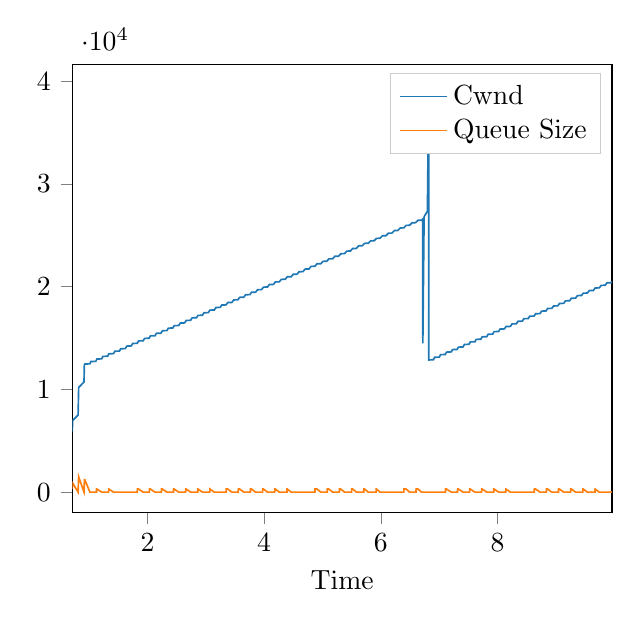
\begin{tikzpicture}

\definecolor{color0}{rgb}{0.12156862745098,0.466666666666667,0.705882352941177}
\definecolor{color1}{rgb}{1,0.498039215686275,0.0549019607843137}

\begin{axis}[
xlabel={Time},
xmin=0.712118, xmax=9.96158,
ymin=-1983.2, ymax=41647.2,
tick align=outside,
tick pos=left,
x grid style={lightgray!92.026143790849673!black},
y grid style={lightgray!92.026143790849673!black},
legend cell align={left},
legend entries={{Cwnd},{Queue Size}},
legend style={draw=white!80.0!black}
]
\addlegendimage{no markers, color0}
\addlegendimage{no markers, color1}
\addplot [semithick, color0]
table {%
0.712118 5896
0.714006 6432
0.715894 6968
0.811261 7504
0.813149 8040
0.815037 8576
0.816925 9112
0.818813 9648
0.820701 10184
0.912291 10720
0.914179 11256
0.916067 11792
0.917955 12328
0.917955 12351
0.919843 12374
0.921731 12397
0.923619 12420
0.925507 12443
0.927395 12466
1.01332 12489
1.01521 12512
1.0171 12534
1.01899 12556
1.02087 12578
1.02276 12600
1.02465 12622
1.02654 12644
1.02843 12666
1.03031 12688
1.0322 12710
1.11435 12732
1.11624 12754
1.11813 12776
1.12002 12798
1.1219 12820
1.12379 12842
1.12568 12864
1.12757 12886
1.12946 12908
1.13134 12930
1.13323 12952
1.21538 12974
1.21727 12996
1.21916 13018
1.22105 13040
1.22293 13062
1.22482 13083
1.22671 13104
1.2286 13125
1.23049 13146
1.23237 13167
1.23426 13188
1.23615 13209
1.31736 13230
1.31924 13251
1.32113 13272
1.32302 13293
1.32491 13314
1.3268 13335
1.32868 13356
1.33057 13377
1.33246 13398
1.33435 13419
1.33624 13440
1.33812 13461
1.41933 13482
1.42122 13503
1.42311 13524
1.425 13545
1.42688 13566
1.42877 13587
1.43066 13608
1.43255 13629
1.43444 13650
1.43632 13671
1.43821 13692
1.4401 13712
1.52036 13732
1.52225 13752
1.52414 13772
1.52603 13792
1.52791 13812
1.5298 13832
1.53169 13852
1.53358 13872
1.53547 13892
1.53735 13912
1.53924 13932
1.54113 13952
1.62139 13972
1.62328 13992
1.62517 14012
1.62706 14032
1.62894 14052
1.63083 14072
1.63272 14092
1.63461 14112
1.6365 14132
1.63838 14152
1.64027 14172
1.64216 14192
1.64405 14212
1.72337 14232
1.72525 14252
1.72714 14272
1.72903 14292
1.73092 14312
1.73281 14332
1.73469 14352
1.73658 14372
1.73847 14391
1.74036 14410
1.74225 14429
1.74413 14448
1.74602 14467
1.82534 14486
1.82723 14505
1.82912 14524
1.831 14543
1.83289 14562
1.83478 14581
1.83667 14600
1.83856 14619
1.84044 14638
1.84233 14657
1.84422 14676
1.84611 14695
1.848 14714
1.92732 14733
1.9292 14752
1.93109 14771
1.93298 14790
1.93487 14809
1.93676 14828
1.93864 14847
1.94053 14866
1.94242 14885
1.94431 14904
1.9462 14923
1.94808 14942
1.94997 14961
2.02835 14980
2.03023 14999
2.03212 15018
2.03401 15037
2.0359 15056
2.03779 15075
2.03967 15094
2.04156 15113
2.04345 15132
2.04534 15150
2.04723 15168
2.04911 15186
2.051 15204
2.12938 15222
2.13126 15240
2.13315 15258
2.13504 15276
2.13693 15294
2.13882 15312
2.1407 15330
2.14259 15348
2.14448 15366
2.14637 15384
2.14826 15402
2.15014 15420
2.15203 15438
2.15392 15456
2.23135 15474
2.23324 15492
2.23513 15510
2.23701 15528
2.2389 15546
2.24079 15564
2.24268 15582
2.24457 15600
2.24645 15618
2.24834 15636
2.25023 15654
2.25212 15672
2.25401 15690
2.25589 15708
2.33332 15726
2.33521 15744
2.3371 15762
2.33899 15780
2.34088 15798
2.34276 15816
2.34465 15834
2.34654 15852
2.34843 15870
2.35032 15888
2.3522 15906
2.35409 15924
2.35598 15942
2.35787 15960
2.43436 15978
2.43624 15995
2.43813 16012
2.44002 16029
2.44191 16046
2.4438 16063
2.44568 16080
2.44757 16097
2.44946 16114
2.45135 16131
2.45324 16148
2.45512 16165
2.45701 16182
2.4589 16199
2.53539 16216
2.53727 16233
2.53916 16250
2.54105 16267
2.54294 16284
2.54483 16301
2.54671 16318
2.5486 16335
2.55049 16352
2.55238 16369
2.55427 16386
2.55615 16403
2.55804 16420
2.55993 16437
2.56182 16454
2.63736 16471
2.63925 16488
2.64114 16505
2.64302 16522
2.64491 16539
2.6468 16556
2.64869 16573
2.65058 16590
2.65246 16607
2.65435 16624
2.65624 16641
2.65813 16658
2.66002 16675
2.6619 16692
2.66379 16709
2.73933 16726
2.74122 16743
2.74311 16760
2.745 16777
2.74689 16794
2.74877 16811
2.75066 16828
2.75255 16845
2.75444 16862
2.75633 16879
2.75821 16896
2.7601 16913
2.76199 16929
2.76388 16945
2.76577 16961
2.84036 16977
2.84225 16993
2.84414 17009
2.84603 17025
2.84792 17041
2.8498 17057
2.85169 17073
2.85358 17089
2.85547 17105
2.85736 17121
2.85924 17137
2.86113 17153
2.86302 17169
2.86491 17185
2.8668 17201
2.9414 17217
2.94328 17233
2.94517 17249
2.94706 17265
2.94895 17281
2.95084 17297
2.95272 17313
2.95461 17329
2.9565 17345
2.95839 17361
2.96028 17377
2.96216 17393
2.96405 17409
2.96594 17425
2.96783 17441
2.96972 17457
3.04337 17473
3.04526 17489
3.04715 17505
3.04903 17521
3.05092 17537
3.05281 17553
3.0547 17569
3.05659 17585
3.05847 17601
3.06036 17617
3.06225 17633
3.06414 17649
3.06603 17665
3.06791 17681
3.0698 17697
3.07169 17713
3.14534 17729
3.14723 17745
3.14912 17761
3.15101 17777
3.1529 17793
3.15478 17809
3.15667 17825
3.15856 17841
3.16045 17857
3.16234 17873
3.16422 17889
3.16611 17905
3.168 17921
3.16989 17937
3.17178 17953
3.17366 17969
3.24637 17984
3.24826 17999
3.25015 18014
3.25204 18029
3.25393 18044
3.25581 18059
3.2577 18074
3.25959 18089
3.26148 18104
3.26337 18119
3.26525 18134
3.26714 18149
3.26903 18164
3.27092 18179
3.27281 18194
3.27469 18209
3.3474 18224
3.34929 18239
3.35118 18254
3.35307 18269
3.35496 18284
3.35684 18299
3.35873 18314
3.36062 18329
3.36251 18344
3.3644 18359
3.36628 18374
3.36817 18389
3.37006 18404
3.37195 18419
3.37384 18434
3.37572 18449
3.44844 18464
3.45032 18479
3.45221 18494
3.4541 18509
3.45599 18524
3.45788 18539
3.45976 18554
3.46165 18569
3.46354 18584
3.46543 18599
3.46732 18614
3.4692 18629
3.47109 18644
3.47298 18659
3.47487 18674
3.47676 18689
3.47864 18704
3.55041 18719
3.5523 18734
3.55419 18749
3.55607 18764
3.55796 18779
3.55985 18794
3.56174 18809
3.56363 18824
3.56551 18839
3.5674 18854
3.56929 18869
3.57118 18884
3.57307 18899
3.57495 18914
3.57684 18929
3.57873 18944
3.58062 18959
3.65238 18974
3.65427 18989
3.65616 19004
3.65805 19019
3.65994 19034
3.66182 19049
3.66371 19064
3.6656 19079
3.66749 19094
3.66938 19109
3.67126 19124
3.67315 19139
3.67504 19154
3.67693 19168
3.67882 19182
3.6807 19196
3.68259 19210
3.75341 19224
3.7553 19238
3.75719 19252
3.75908 19266
3.76097 19280
3.76285 19294
3.76474 19308
3.76663 19322
3.76852 19336
3.77041 19350
3.77229 19364
3.77418 19378
3.77607 19392
3.77796 19406
3.77985 19420
3.78173 19434
3.78362 19448
3.85444 19462
3.85633 19476
3.85822 19490
3.86011 19504
3.862 19518
3.86388 19532
3.86577 19546
3.86766 19560
3.86955 19574
3.87144 19588
3.87332 19602
3.87521 19616
3.8771 19630
3.87899 19644
3.88088 19658
3.88276 19672
3.88465 19686
3.88654 19700
3.95642 19714
3.95831 19728
3.9602 19742
3.96208 19756
3.96397 19770
3.96586 19784
3.96775 19798
3.96964 19812
3.97152 19826
3.97341 19840
3.9753 19854
3.97719 19868
3.97908 19882
3.98096 19896
3.98285 19910
3.98474 19924
3.98663 19938
3.98852 19952
4.05839 19966
4.06028 19980
4.06217 19994
4.06406 20008
4.06595 20022
4.06783 20036
4.06972 20050
4.07161 20064
4.0735 20078
4.07539 20092
4.07727 20106
4.07916 20120
4.08105 20134
4.08294 20148
4.08483 20162
4.08671 20176
4.0886 20190
4.09049 20204
4.15942 20218
4.16131 20232
4.1632 20246
4.16509 20260
4.16698 20274
4.16886 20288
4.17075 20302
4.17264 20316
4.17453 20330
4.17642 20344
4.1783 20358
4.18019 20372
4.18208 20386
4.18397 20400
4.18586 20414
4.18774 20428
4.18963 20442
4.19152 20456
4.26045 20470
4.26234 20484
4.26423 20498
4.26612 20512
4.26801 20526
4.26989 20539
4.27178 20552
4.27367 20565
4.27556 20578
4.27745 20591
4.27933 20604
4.28122 20617
4.28311 20630
4.285 20643
4.28689 20656
4.28877 20669
4.29066 20682
4.29255 20695
4.29444 20708
4.36243 20721
4.36432 20734
4.3662 20747
4.36809 20760
4.36998 20773
4.37187 20786
4.37376 20799
4.37564 20812
4.37753 20825
4.37942 20838
4.38131 20851
4.3832 20864
4.38508 20877
4.38697 20890
4.38886 20903
4.39075 20916
4.39264 20929
4.39452 20942
4.39641 20955
4.4644 20968
4.46629 20981
4.46818 20994
4.47007 21007
4.47196 21020
4.47384 21033
4.47573 21046
4.47762 21059
4.47951 21072
4.4814 21085
4.48328 21098
4.48517 21111
4.48706 21124
4.48895 21137
4.49084 21150
4.49272 21163
4.49461 21176
4.4965 21189
4.49839 21202
4.56543 21215
4.56732 21228
4.56921 21241
4.5711 21254
4.57299 21267
4.57487 21280
4.57676 21293
4.57865 21306
4.58054 21319
4.58243 21332
4.58431 21345
4.5862 21358
4.58809 21371
4.58998 21384
4.59187 21397
4.59375 21410
4.59564 21423
4.59753 21436
4.59942 21449
4.66646 21462
4.66835 21475
4.67024 21488
4.67213 21501
4.67402 21514
4.6759 21527
4.67779 21540
4.67968 21553
4.68157 21566
4.68346 21579
4.68534 21592
4.68723 21605
4.68912 21618
4.69101 21631
4.6929 21644
4.69478 21657
4.69667 21670
4.69856 21683
4.70045 21696
4.70234 21709
4.76844 21722
4.77033 21735
4.77221 21748
4.7741 21761
4.77599 21774
4.77788 21787
4.77977 21800
4.78165 21813
4.78354 21826
4.78543 21839
4.78732 21852
4.78921 21865
4.79109 21878
4.79298 21891
4.79487 21904
4.79676 21917
4.79865 21930
4.80053 21943
4.80242 21956
4.80431 21969
4.87041 21982
4.8723 21995
4.87419 22008
4.87608 22021
4.87796 22034
4.87985 22047
4.88174 22060
4.88363 22073
4.88552 22086
4.8874 22099
4.88929 22112
4.89118 22124
4.89307 22136
4.89496 22148
4.89684 22160
4.89873 22172
4.90062 22184
4.90251 22196
4.9044 22208
4.90628 22220
4.97239 22232
4.97428 22244
4.97616 22256
4.97805 22268
4.97994 22280
4.98183 22292
4.98372 22304
4.9856 22316
4.98749 22328
4.98938 22340
4.99127 22352
4.99316 22364
4.99504 22376
4.99693 22388
4.99882 22400
5.00071 22412
5.0026 22424
5.00448 22436
5.00637 22448
5.00826 22460
5.07342 22472
5.07531 22484
5.07719 22496
5.07908 22508
5.08097 22520
5.08286 22532
5.08475 22544
5.08663 22556
5.08852 22568
5.09041 22580
5.0923 22592
5.09419 22604
5.09607 22616
5.09796 22628
5.09985 22640
5.10174 22652
5.10363 22664
5.10551 22676
5.1074 22688
5.10929 22700
5.17445 22712
5.17634 22724
5.17822 22736
5.18011 22748
5.182 22760
5.18389 22772
5.18578 22784
5.18766 22796
5.18955 22808
5.19144 22820
5.19333 22832
5.19522 22844
5.1971 22856
5.19899 22868
5.20088 22880
5.20277 22892
5.20466 22904
5.20654 22916
5.20843 22928
5.21032 22940
5.21221 22952
5.27642 22964
5.27831 22976
5.2802 22988
5.28209 23000
5.28397 23012
5.28586 23024
5.28775 23036
5.28964 23048
5.29153 23060
5.29341 23072
5.2953 23084
5.29719 23096
5.29908 23108
5.30097 23120
5.30285 23132
5.30474 23144
5.30663 23156
5.30852 23168
5.31041 23180
5.31229 23192
5.31418 23204
5.3784 23216
5.38028 23228
5.38217 23240
5.38406 23252
5.38595 23264
5.38784 23276
5.38972 23288
5.39161 23300
5.3935 23312
5.39539 23324
5.39728 23336
5.39916 23348
5.40105 23360
5.40294 23372
5.40483 23384
5.40672 23396
5.4086 23408
5.41049 23420
5.41238 23432
5.41427 23444
5.41616 23456
5.47943 23468
5.48132 23480
5.4832 23492
5.48509 23504
5.48698 23516
5.48887 23528
5.49076 23540
5.49264 23552
5.49453 23564
5.49642 23576
5.49831 23588
5.5002 23600
5.50208 23612
5.50397 23624
5.50586 23636
5.50775 23648
5.50964 23660
5.51152 23672
5.51341 23684
5.5153 23696
5.51719 23708
5.58046 23720
5.58235 23732
5.58423 23744
5.58612 23756
5.58801 23768
5.5899 23780
5.59179 23792
5.59367 23804
5.59556 23816
5.59745 23828
5.59934 23840
5.60123 23852
5.60311 23864
5.605 23876
5.60689 23888
5.60878 23900
5.61067 23912
5.61255 23924
5.61444 23936
5.61633 23948
5.61822 23959
5.62011 23970
5.68243 23981
5.68432 23992
5.68621 24003
5.6881 24014
5.68998 24025
5.69187 24036
5.69376 24047
5.69565 24058
5.69754 24069
5.69942 24080
5.70131 24091
5.7032 24102
5.70509 24113
5.70698 24124
5.70886 24135
5.71075 24146
5.71264 24157
5.71453 24168
5.71642 24179
5.7183 24190
5.72019 24201
5.72208 24212
5.78441 24223
5.78629 24234
5.78818 24245
5.79007 24256
5.79196 24267
5.79385 24278
5.79573 24289
5.79762 24300
5.79951 24311
5.8014 24322
5.80329 24333
5.80517 24344
5.80706 24355
5.80895 24366
5.81084 24377
5.81273 24388
5.81461 24399
5.8165 24410
5.81839 24421
5.82028 24432
5.82217 24443
5.82405 24454
5.88544 24465
5.88732 24476
5.88921 24487
5.8911 24498
5.89299 24509
5.89488 24520
5.89676 24531
5.89865 24542
5.90054 24553
5.90243 24564
5.90432 24575
5.9062 24586
5.90809 24597
5.90998 24608
5.91187 24619
5.91376 24630
5.91564 24641
5.91753 24652
5.91942 24663
5.92131 24674
5.9232 24685
5.92508 24696
5.98647 24707
5.98836 24718
5.99024 24729
5.99213 24740
5.99402 24751
5.99591 24762
5.9978 24773
5.99968 24784
6.00157 24795
6.00346 24806
6.00535 24817
6.00724 24828
6.00912 24839
6.01101 24850
6.0129 24861
6.01479 24872
6.01668 24883
6.01856 24894
6.02045 24905
6.02234 24916
6.02423 24927
6.02612 24938
6.028 24949
6.08844 24960
6.09033 24971
6.09222 24982
6.09411 24993
6.09599 25004
6.09788 25015
6.09977 25026
6.10166 25037
6.10355 25048
6.10543 25059
6.10732 25070
6.10921 25081
6.1111 25092
6.11299 25103
6.11487 25114
6.11676 25125
6.11865 25136
6.12054 25147
6.12243 25158
6.12431 25169
6.1262 25180
6.12809 25191
6.12998 25202
6.19042 25213
6.1923 25224
6.19419 25235
6.19608 25246
6.19797 25257
6.19986 25268
6.20174 25279
6.20363 25290
6.20552 25301
6.20741 25312
6.2093 25323
6.21118 25334
6.21307 25345
6.21496 25356
6.21685 25367
6.21874 25378
6.22062 25389
6.22251 25400
6.2244 25411
6.22629 25422
6.22818 25433
6.23006 25444
6.23195 25455
6.29145 25466
6.29333 25477
6.29522 25488
6.29711 25499
6.299 25510
6.30089 25521
6.30277 25532
6.30466 25543
6.30655 25554
6.30844 25565
6.31033 25576
6.31221 25587
6.3141 25598
6.31599 25609
6.31788 25620
6.31977 25631
6.32165 25642
6.32354 25653
6.32543 25664
6.32732 25675
6.32921 25686
6.33109 25697
6.33298 25708
6.39248 25719
6.39436 25730
6.39625 25741
6.39814 25752
6.40003 25763
6.40192 25774
6.4038 25785
6.40569 25796
6.40758 25807
6.40947 25818
6.41136 25829
6.41324 25840
6.41513 25851
6.41702 25862
6.41891 25873
6.4208 25884
6.42268 25895
6.42457 25906
6.42646 25917
6.42835 25928
6.43024 25939
6.43212 25950
6.43401 25961
6.49351 25972
6.4954 25983
6.49728 25994
6.49917 26005
6.50106 26016
6.50295 26027
6.50484 26038
6.50672 26049
6.50861 26060
6.5105 26071
6.51239 26082
6.51428 26093
6.51616 26104
6.51805 26115
6.51994 26126
6.52183 26136
6.52372 26146
6.5256 26156
6.52749 26166
6.52938 26176
6.53127 26186
6.53316 26196
6.53504 26206
6.53693 26216
6.59548 26226
6.59737 26236
6.59926 26246
6.60115 26256
6.60303 26266
6.60492 26276
6.60681 26286
6.6087 26296
6.61059 26306
6.61247 26316
6.61436 26326
6.61625 26336
6.61814 26346
6.62003 26356
6.62191 26366
6.6238 26376
6.62569 26386
6.62758 26396
6.62947 26406
6.63135 26416
6.63324 26426
6.63513 26436
6.63702 26446
6.63891 26456
6.69746 26466
6.69934 26476
6.70123 26486
6.70312 26496
6.70501 26506
6.7069 26516
6.70878 26526
6.71067 26536
6.71256 26546
6.71445 26556
6.71634 26566
6.72011 14472
6.72106 15008
6.722 15544
6.72294 16080
6.72389 16616
6.72483 17152
6.72578 17688
6.72672 18224
6.72766 18760
6.72861 19296
6.72955 19832
6.7305 20368
6.73144 20904
6.73238 21440
6.73333 21976
6.73427 22512
6.73522 23048
6.73616 23584
6.7371 24120
6.73805 24656
6.73899 25192
6.73994 25728
6.74088 26264
6.74182 26800
6.79849 27336
6.79943 27872
6.80037 28408
6.80132 28944
6.80226 29480
6.80321 30016
6.80415 30552
6.80509 31088
6.80604 31624
6.80698 32160
6.80793 32696
6.80887 33232
6.80981 33768
6.81076 34304
6.8117 34840
6.81265 35376
6.81359 35912
6.81453 36448
6.81548 36984
6.81642 37520
6.81737 38056
6.81831 38592
6.81925 39128
6.8202 39664
6.82114 12864
6.9014 12886
6.90329 12908
6.90518 12930
6.90707 12952
6.90896 12974
6.91084 12996
6.91273 13018
6.91462 13040
6.91651 13062
6.9184 13083
6.92028 13104
6.92217 13125
7.00338 13146
7.00527 13167
7.00716 13188
7.00904 13209
7.01093 13230
7.01282 13251
7.01471 13272
7.0166 13293
7.01848 13314
7.02037 13335
7.02226 13356
7.02415 13377
7.10535 13398
7.10724 13419
7.10913 13440
7.11102 13461
7.11291 13482
7.11479 13503
7.11668 13524
7.11857 13545
7.12046 13566
7.12235 13587
7.12423 13608
7.12612 13629
7.20733 13650
7.20922 13671
7.2111 13692
7.21299 13712
7.21488 13732
7.21677 13752
7.21866 13772
7.22054 13792
7.22243 13812
7.22432 13832
7.22621 13852
7.2281 13872
7.30836 13892
7.31025 13912
7.31213 13932
7.31402 13952
7.31591 13972
7.3178 13992
7.31969 14012
7.32157 14032
7.32346 14052
7.32535 14072
7.32724 14092
7.32913 14112
7.40939 14132
7.41128 14152
7.41316 14172
7.41505 14192
7.41694 14212
7.41883 14232
7.42072 14252
7.4226 14272
7.42449 14292
7.42638 14312
7.42827 14332
7.43016 14352
7.43204 14372
7.51136 14391
7.51325 14410
7.51514 14429
7.51703 14448
7.51892 14467
7.5208 14486
7.52269 14505
7.52458 14524
7.52647 14543
7.52836 14562
7.53024 14581
7.53213 14600
7.53402 14619
7.61334 14638
7.61523 14657
7.61711 14676
7.619 14695
7.62089 14714
7.62278 14733
7.62467 14752
7.62655 14771
7.62844 14790
7.63033 14809
7.63222 14828
7.63411 14847
7.63599 14866
7.71437 14885
7.71626 14904
7.71814 14923
7.72003 14942
7.72192 14961
7.72381 14980
7.7257 14999
7.72758 15018
7.72947 15037
7.73136 15056
7.73325 15075
7.73514 15094
7.73702 15113
7.8154 15132
7.81729 15150
7.81917 15168
7.82106 15186
7.82295 15204
7.82484 15222
7.82673 15240
7.82861 15258
7.8305 15276
7.83239 15294
7.83428 15312
7.83617 15330
7.83805 15348
7.83994 15366
7.91737 15384
7.91926 15402
7.92115 15420
7.92304 15438
7.92492 15456
7.92681 15474
7.9287 15492
7.93059 15510
7.93248 15528
7.93436 15546
7.93625 15564
7.93814 15582
7.94003 15600
7.94192 15618
8.01935 15636
8.02124 15654
8.02312 15672
8.02501 15690
8.0269 15708
8.02879 15726
8.03068 15744
8.03256 15762
8.03445 15780
8.03634 15798
8.03823 15816
8.04012 15834
8.042 15852
8.04389 15870
8.12038 15888
8.12227 15906
8.12415 15924
8.12604 15942
8.12793 15960
8.12982 15978
8.13171 15995
8.13359 16012
8.13548 16029
8.13737 16046
8.13926 16063
8.14115 16080
8.14303 16097
8.14492 16114
8.22141 16131
8.2233 16148
8.22518 16165
8.22707 16182
8.22896 16199
8.23085 16216
8.23274 16233
8.23462 16250
8.23651 16267
8.2384 16284
8.24029 16301
8.24218 16318
8.24406 16335
8.24595 16352
8.24784 16369
8.32338 16386
8.32527 16403
8.32716 16420
8.32905 16437
8.33093 16454
8.33282 16471
8.33471 16488
8.3366 16505
8.33849 16522
8.34037 16539
8.34226 16556
8.34415 16573
8.34604 16590
8.34793 16607
8.34981 16624
8.42536 16641
8.42724 16658
8.42913 16675
8.43102 16692
8.43291 16709
8.4348 16726
8.43668 16743
8.43857 16760
8.44046 16777
8.44235 16794
8.44424 16811
8.44612 16828
8.44801 16845
8.4499 16862
8.45179 16879
8.52639 16896
8.52828 16913
8.53016 16929
8.53205 16945
8.53394 16961
8.53583 16977
8.53772 16993
8.5396 17009
8.54149 17025
8.54338 17041
8.54527 17057
8.54716 17073
8.54904 17089
8.55093 17105
8.55282 17121
8.62742 17137
8.62931 17153
8.63119 17169
8.63308 17185
8.63497 17201
8.63686 17217
8.63875 17233
8.64063 17249
8.64252 17265
8.64441 17281
8.6463 17297
8.64819 17313
8.65007 17329
8.65196 17345
8.65385 17361
8.72845 17377
8.73034 17393
8.73222 17409
8.73411 17425
8.736 17441
8.73789 17457
8.73978 17473
8.74166 17489
8.74355 17505
8.74544 17521
8.74733 17537
8.74922 17553
8.7511 17569
8.75299 17585
8.75488 17601
8.75677 17617
8.83042 17633
8.83231 17649
8.8342 17665
8.83609 17681
8.83797 17697
8.83986 17713
8.84175 17729
8.84364 17745
8.84553 17761
8.84741 17777
8.8493 17793
8.85119 17809
8.85308 17825
8.85497 17841
8.85685 17857
8.85874 17873
8.9324 17889
8.93428 17905
8.93617 17921
8.93806 17937
8.93995 17953
8.94184 17969
8.94372 17984
8.94561 17999
8.9475 18014
8.94939 18029
8.95128 18044
8.95316 18059
8.95505 18074
8.95694 18089
8.95883 18104
8.96072 18119
9.03343 18134
9.03532 18149
9.0372 18164
9.03909 18179
9.04098 18194
9.04287 18209
9.04476 18224
9.04664 18239
9.04853 18254
9.05042 18269
9.05231 18284
9.0542 18299
9.05608 18314
9.05797 18329
9.05986 18344
9.06175 18359
9.13446 18374
9.13635 18389
9.13823 18404
9.14012 18419
9.14201 18434
9.1439 18449
9.14579 18464
9.14767 18479
9.14956 18494
9.15145 18509
9.15334 18524
9.15523 18539
9.15711 18554
9.159 18569
9.16089 18584
9.16278 18599
9.16467 18614
9.23643 18629
9.23832 18644
9.24021 18659
9.2421 18674
9.24398 18689
9.24587 18704
9.24776 18719
9.24965 18734
9.25154 18749
9.25342 18764
9.25531 18779
9.2572 18794
9.25909 18809
9.26098 18824
9.26286 18839
9.26475 18854
9.26664 18869
9.33841 18884
9.34029 18899
9.34218 18914
9.34407 18929
9.34596 18944
9.34785 18959
9.34973 18974
9.35162 18989
9.35351 19004
9.3554 19019
9.35729 19034
9.35917 19049
9.36106 19064
9.36295 19079
9.36484 19094
9.36673 19109
9.36861 19124
9.43944 19139
9.44132 19154
9.44321 19168
9.4451 19182
9.44699 19196
9.44888 19210
9.45076 19224
9.45265 19238
9.45454 19252
9.45643 19266
9.45832 19280
9.4602 19294
9.46209 19308
9.46398 19322
9.46587 19336
9.46776 19350
9.46964 19364
9.54047 19378
9.54236 19392
9.54424 19406
9.54613 19420
9.54802 19434
9.54991 19448
9.5518 19462
9.55368 19476
9.55557 19490
9.55746 19504
9.55935 19518
9.56124 19532
9.56312 19546
9.56501 19560
9.5669 19574
9.56879 19588
9.57068 19602
9.57256 19616
9.64244 19630
9.64433 19644
9.64622 19658
9.64811 19672
9.64999 19686
9.65188 19700
9.65377 19714
9.65566 19728
9.65755 19742
9.65943 19756
9.66132 19770
9.66321 19784
9.6651 19798
9.66699 19812
9.66887 19826
9.67076 19840
9.67265 19854
9.67454 19868
9.74442 19882
9.7463 19896
9.74819 19910
9.75008 19924
9.75197 19938
9.75386 19952
9.75574 19966
9.75763 19980
9.75952 19994
9.76141 20008
9.7633 20022
9.76518 20036
9.76707 20050
9.76896 20064
9.77085 20078
9.77274 20092
9.77462 20106
9.77651 20120
9.84545 20134
9.84733 20148
9.84922 20162
9.85111 20176
9.853 20190
9.85489 20204
9.85677 20218
9.85866 20232
9.86055 20246
9.86244 20260
9.86433 20274
9.86621 20288
9.8681 20302
9.86999 20316
9.87188 20330
9.87377 20344
9.87565 20358
9.87754 20372
9.94648 20386
9.94836 20400
9.95025 20414
9.95214 20428
9.95403 20442
9.95592 20456
9.9578 20470
9.95969 20484
9.96158 20498
};
\addplot [semithick, color1]
table {%
0.712118 300
0.714006 600
0.715894 900
0.811261 0
0.813149 300
0.815037 600
0.816925 900
0.818813 1200
0.820701 1500
0.912291 0
0.914179 300
0.916067 600
0.917955 900
0.917955 900
0.919843 1200
0.921731 1200
0.923619 1200
0.925507 1200
0.927395 1200
1.01332 0
1.01521 0
1.0171 0
1.01899 0
1.02087 0
1.02276 0
1.02465 0
1.02654 0
1.02843 0
1.03031 0
1.0322 0
1.11435 0
1.11624 0
1.11813 0
1.12002 0
1.1219 0
1.12379 0
1.12568 0
1.12757 300
1.12946 300
1.13134 300
1.13323 300
1.21538 0
1.21727 0
1.21916 0
1.22105 0
1.22293 0
1.22482 0
1.22671 0
1.2286 0
1.23049 0
1.23237 0
1.23426 0
1.23615 0
1.31736 0
1.31924 0
1.32113 0
1.32302 0
1.32491 0
1.3268 0
1.32868 0
1.33057 0
1.33246 0
1.33435 0
1.33624 300
1.33812 300
1.41933 0
1.42122 0
1.42311 0
1.425 0
1.42688 0
1.42877 0
1.43066 0
1.43255 0
1.43444 0
1.43632 0
1.43821 0
1.4401 0
1.52036 0
1.52225 0
1.52414 0
1.52603 0
1.52791 0
1.5298 0
1.53169 0
1.53358 0
1.53547 0
1.53735 0
1.53924 0
1.54113 0
1.62139 0
1.62328 0
1.62517 0
1.62706 0
1.62894 0
1.63083 0
1.63272 0
1.63461 0
1.6365 0
1.63838 0
1.64027 0
1.64216 0
1.64405 0
1.72337 0
1.72525 0
1.72714 0
1.72903 0
1.73092 0
1.73281 0
1.73469 0
1.73658 0
1.73847 0
1.74036 0
1.74225 0
1.74413 0
1.74602 0
1.82534 0
1.82723 300
1.82912 300
1.831 300
1.83289 300
1.83478 300
1.83667 300
1.83856 300
1.84044 300
1.84233 300
1.84422 300
1.84611 300
1.848 300
1.92732 0
1.9292 0
1.93109 0
1.93298 0
1.93487 0
1.93676 0
1.93864 0
1.94053 0
1.94242 0
1.94431 0
1.9462 0
1.94808 0
1.94997 0
2.02835 0
2.03023 0
2.03212 0
2.03401 300
2.0359 300
2.03779 300
2.03967 300
2.04156 300
2.04345 300
2.04534 300
2.04723 300
2.04911 300
2.051 300
2.12938 0
2.13126 0
2.13315 0
2.13504 0
2.13693 0
2.13882 0
2.1407 0
2.14259 0
2.14448 0
2.14637 0
2.14826 0
2.15014 0
2.15203 0
2.15392 0
2.23135 0
2.23324 0
2.23513 0
2.23701 0
2.2389 0
2.24079 300
2.24268 300
2.24457 300
2.24645 300
2.24834 300
2.25023 300
2.25212 300
2.25401 300
2.25589 300
2.33332 0
2.33521 0
2.3371 0
2.33899 0
2.34088 0
2.34276 0
2.34465 0
2.34654 0
2.34843 0
2.35032 0
2.3522 0
2.35409 0
2.35598 0
2.35787 0
2.43436 0
2.43624 0
2.43813 0
2.44002 0
2.44191 0
2.4438 0
2.44568 0
2.44757 300
2.44946 300
2.45135 300
2.45324 300
2.45512 300
2.45701 300
2.4589 300
2.53539 0
2.53727 0
2.53916 0
2.54105 0
2.54294 0
2.54483 0
2.54671 0
2.5486 0
2.55049 0
2.55238 0
2.55427 0
2.55615 0
2.55804 0
2.55993 0
2.56182 0
2.63736 0
2.63925 0
2.64114 0
2.64302 0
2.64491 0
2.6468 0
2.64869 0
2.65058 0
2.65246 0
2.65435 0
2.65624 300
2.65813 300
2.66002 300
2.6619 300
2.66379 300
2.73933 0
2.74122 0
2.74311 0
2.745 0
2.74689 0
2.74877 0
2.75066 0
2.75255 0
2.75444 0
2.75633 0
2.75821 0
2.7601 0
2.76199 0
2.76388 0
2.76577 0
2.84036 0
2.84225 0
2.84414 0
2.84603 0
2.84792 0
2.8498 0
2.85169 0
2.85358 0
2.85547 0
2.85736 0
2.85924 0
2.86113 0
2.86302 300
2.86491 300
2.8668 300
2.9414 0
2.94328 0
2.94517 0
2.94706 0
2.94895 0
2.95084 0
2.95272 0
2.95461 0
2.9565 0
2.95839 0
2.96028 0
2.96216 0
2.96405 0
2.96594 0
2.96783 0
2.96972 0
3.04337 0
3.04526 0
3.04715 0
3.04903 0
3.05092 0
3.05281 0
3.0547 0
3.05659 0
3.05847 0
3.06036 0
3.06225 0
3.06414 0
3.06603 0
3.06791 0
3.0698 0
3.07169 300
3.14534 0
3.14723 0
3.14912 0
3.15101 0
3.1529 0
3.15478 0
3.15667 0
3.15856 0
3.16045 0
3.16234 0
3.16422 0
3.16611 0
3.168 0
3.16989 0
3.17178 0
3.17366 0
3.24637 0
3.24826 0
3.25015 0
3.25204 0
3.25393 0
3.25581 0
3.2577 0
3.25959 0
3.26148 0
3.26337 0
3.26525 0
3.26714 0
3.26903 0
3.27092 0
3.27281 0
3.27469 0
3.3474 0
3.34929 300
3.35118 300
3.35307 300
3.35496 300
3.35684 300
3.35873 300
3.36062 300
3.36251 300
3.3644 300
3.36628 300
3.36817 300
3.37006 300
3.37195 300
3.37384 300
3.37572 300
3.44844 0
3.45032 0
3.45221 0
3.4541 0
3.45599 0
3.45788 0
3.45976 0
3.46165 0
3.46354 0
3.46543 0
3.46732 0
3.4692 0
3.47109 0
3.47298 0
3.47487 0
3.47676 0
3.47864 0
3.55041 0
3.5523 0
3.55419 0
3.55607 0
3.55796 300
3.55985 300
3.56174 300
3.56363 300
3.56551 300
3.5674 300
3.56929 300
3.57118 300
3.57307 300
3.57495 300
3.57684 300
3.57873 300
3.58062 300
3.65238 0
3.65427 0
3.65616 0
3.65805 0
3.65994 0
3.66182 0
3.66371 0
3.6656 0
3.66749 0
3.66938 0
3.67126 0
3.67315 0
3.67504 0
3.67693 0
3.67882 0
3.6807 0
3.68259 0
3.75341 0
3.7553 0
3.75719 0
3.75908 0
3.76097 0
3.76285 0
3.76474 0
3.76663 300
3.76852 300
3.77041 300
3.77229 300
3.77418 300
3.77607 300
3.77796 300
3.77985 300
3.78173 300
3.78362 300
3.85444 0
3.85633 0
3.85822 0
3.86011 0
3.862 0
3.86388 0
3.86577 0
3.86766 0
3.86955 0
3.87144 0
3.87332 0
3.87521 0
3.8771 0
3.87899 0
3.88088 0
3.88276 0
3.88465 0
3.88654 0
3.95642 0
3.95831 0
3.9602 0
3.96208 0
3.96397 0
3.96586 0
3.96775 0
3.96964 0
3.97152 0
3.97341 0
3.9753 300
3.97719 300
3.97908 300
3.98096 300
3.98285 300
3.98474 300
3.98663 300
3.98852 300
4.05839 0
4.06028 0
4.06217 0
4.06406 0
4.06595 0
4.06783 0
4.06972 0
4.07161 0
4.0735 0
4.07539 0
4.07727 0
4.07916 0
4.08105 0
4.08294 0
4.08483 0
4.08671 0
4.0886 0
4.09049 0
4.15942 0
4.16131 0
4.1632 0
4.16509 0
4.16698 0
4.16886 0
4.17075 0
4.17264 0
4.17453 0
4.17642 0
4.1783 0
4.18019 0
4.18208 300
4.18397 300
4.18586 300
4.18774 300
4.18963 300
4.19152 300
4.26045 0
4.26234 0
4.26423 0
4.26612 0
4.26801 0
4.26989 0
4.27178 0
4.27367 0
4.27556 0
4.27745 0
4.27933 0
4.28122 0
4.28311 0
4.285 0
4.28689 0
4.28877 0
4.29066 0
4.29255 0
4.29444 0
4.36243 0
4.36432 0
4.3662 0
4.36809 0
4.36998 0
4.37187 0
4.37376 0
4.37564 0
4.37753 0
4.37942 0
4.38131 0
4.3832 0
4.38508 0
4.38697 0
4.38886 0
4.39075 0
4.39264 300
4.39452 300
4.39641 300
4.4644 0
4.46629 0
4.46818 0
4.47007 0
4.47196 0
4.47384 0
4.47573 0
4.47762 0
4.47951 0
4.4814 0
4.48328 0
4.48517 0
4.48706 0
4.48895 0
4.49084 0
4.49272 0
4.49461 0
4.4965 0
4.49839 0
4.56543 0
4.56732 0
4.56921 0
4.5711 0
4.57299 0
4.57487 0
4.57676 0
4.57865 0
4.58054 0
4.58243 0
4.58431 0
4.5862 0
4.58809 0
4.58998 0
4.59187 0
4.59375 0
4.59564 0
4.59753 0
4.59942 0
4.66646 0
4.66835 0
4.67024 0
4.67213 0
4.67402 0
4.6759 0
4.67779 0
4.67968 0
4.68157 0
4.68346 0
4.68534 0
4.68723 0
4.68912 0
4.69101 0
4.6929 0
4.69478 0
4.69667 0
4.69856 0
4.70045 0
4.70234 0
4.76844 0
4.77033 0
4.77221 0
4.7741 0
4.77599 0
4.77788 0
4.77977 0
4.78165 0
4.78354 0
4.78543 0
4.78732 0
4.78921 0
4.79109 0
4.79298 0
4.79487 0
4.79676 0
4.79865 0
4.80053 0
4.80242 0
4.80431 0
4.87041 0
4.8723 300
4.87419 300
4.87608 300
4.87796 300
4.87985 300
4.88174 300
4.88363 300
4.88552 300
4.8874 300
4.88929 300
4.89118 300
4.89307 300
4.89496 300
4.89684 300
4.89873 300
4.90062 300
4.90251 300
4.9044 300
4.90628 300
4.97239 0
4.97428 0
4.97616 0
4.97805 0
4.97994 0
4.98183 0
4.98372 0
4.9856 0
4.98749 0
4.98938 0
4.99127 0
4.99316 0
4.99504 0
4.99693 0
4.99882 0
5.00071 0
5.0026 0
5.00448 0
5.00637 0
5.00826 0
5.07342 0
5.07531 0
5.07719 0
5.07908 0
5.08097 0
5.08286 300
5.08475 300
5.08663 300
5.08852 300
5.09041 300
5.0923 300
5.09419 300
5.09607 300
5.09796 300
5.09985 300
5.10174 300
5.10363 300
5.10551 300
5.1074 300
5.10929 300
5.17445 0
5.17634 0
5.17822 0
5.18011 0
5.182 0
5.18389 0
5.18578 0
5.18766 0
5.18955 0
5.19144 0
5.19333 0
5.19522 0
5.1971 0
5.19899 0
5.20088 0
5.20277 0
5.20466 0
5.20654 0
5.20843 0
5.21032 0
5.21221 0
5.27642 0
5.27831 0
5.2802 0
5.28209 0
5.28397 0
5.28586 0
5.28775 0
5.28964 0
5.29153 300
5.29341 300
5.2953 300
5.29719 300
5.29908 300
5.30097 300
5.30285 300
5.30474 300
5.30663 300
5.30852 300
5.31041 300
5.31229 300
5.31418 300
5.3784 0
5.38028 0
5.38217 0
5.38406 0
5.38595 0
5.38784 0
5.38972 0
5.39161 0
5.3935 0
5.39539 0
5.39728 0
5.39916 0
5.40105 0
5.40294 0
5.40483 0
5.40672 0
5.4086 0
5.41049 0
5.41238 0
5.41427 0
5.41616 0
5.47943 0
5.48132 0
5.4832 0
5.48509 0
5.48698 0
5.48887 0
5.49076 0
5.49264 0
5.49453 0
5.49642 0
5.49831 0
5.5002 300
5.50208 300
5.50397 300
5.50586 300
5.50775 300
5.50964 300
5.51152 300
5.51341 300
5.5153 300
5.51719 300
5.58046 0
5.58235 0
5.58423 0
5.58612 0
5.58801 0
5.5899 0
5.59179 0
5.59367 0
5.59556 0
5.59745 0
5.59934 0
5.60123 0
5.60311 0
5.605 0
5.60689 0
5.60878 0
5.61067 0
5.61255 0
5.61444 0
5.61633 0
5.61822 0
5.62011 0
5.68243 0
5.68432 0
5.68621 0
5.6881 0
5.68998 0
5.69187 0
5.69376 0
5.69565 0
5.69754 0
5.69942 0
5.70131 0
5.7032 0
5.70509 0
5.70698 0
5.70886 300
5.71075 300
5.71264 300
5.71453 300
5.71642 300
5.7183 300
5.72019 300
5.72208 300
5.78441 0
5.78629 0
5.78818 0
5.79007 0
5.79196 0
5.79385 0
5.79573 0
5.79762 0
5.79951 0
5.8014 0
5.80329 0
5.80517 0
5.80706 0
5.80895 0
5.81084 0
5.81273 0
5.81461 0
5.8165 0
5.81839 0
5.82028 0
5.82217 0
5.82405 0
5.88544 0
5.88732 0
5.88921 0
5.8911 0
5.89299 0
5.89488 0
5.89676 0
5.89865 0
5.90054 0
5.90243 0
5.90432 0
5.9062 0
5.90809 0
5.90998 0
5.91187 0
5.91376 0
5.91564 0
5.91753 0
5.91942 0
5.92131 300
5.9232 300
5.92508 300
5.98647 0
5.98836 0
5.99024 0
5.99213 0
5.99402 0
5.99591 0
5.9978 0
5.99968 0
6.00157 0
6.00346 0
6.00535 0
6.00724 0
6.00912 0
6.01101 0
6.0129 0
6.01479 0
6.01668 0
6.01856 0
6.02045 0
6.02234 0
6.02423 0
6.02612 0
6.028 0
6.08844 0
6.09033 0
6.09222 0
6.09411 0
6.09599 0
6.09788 0
6.09977 0
6.10166 0
6.10355 0
6.10543 0
6.10732 0
6.10921 0
6.1111 0
6.11299 0
6.11487 0
6.11676 0
6.11865 0
6.12054 0
6.12243 0
6.12431 0
6.1262 0
6.12809 0
6.12998 0
6.19042 0
6.1923 0
6.19419 0
6.19608 0
6.19797 0
6.19986 0
6.20174 0
6.20363 0
6.20552 0
6.20741 0
6.2093 0
6.21118 0
6.21307 0
6.21496 0
6.21685 0
6.21874 0
6.22062 0
6.22251 0
6.2244 0
6.22629 0
6.22818 0
6.23006 0
6.23195 0
6.29145 0
6.29333 0
6.29522 0
6.29711 0
6.299 0
6.30089 0
6.30277 0
6.30466 0
6.30655 0
6.30844 0
6.31033 0
6.31221 0
6.3141 0
6.31599 0
6.31788 0
6.31977 0
6.32165 0
6.32354 0
6.32543 0
6.32732 0
6.32921 0
6.33109 0
6.33298 0
6.39248 0
6.39436 0
6.39625 300
6.39814 300
6.40003 300
6.40192 300
6.4038 300
6.40569 300
6.40758 300
6.40947 300
6.41136 300
6.41324 300
6.41513 300
6.41702 300
6.41891 300
6.4208 300
6.42268 300
6.42457 300
6.42646 300
6.42835 300
6.43024 300
6.43212 300
6.43401 300
6.49351 0
6.4954 0
6.49728 0
6.49917 0
6.50106 0
6.50295 0
6.50484 0
6.50672 0
6.50861 0
6.5105 0
6.51239 0
6.51428 0
6.51616 0
6.51805 0
6.51994 0
6.52183 0
6.52372 0
6.5256 0
6.52749 0
6.52938 0
6.53127 0
6.53316 0
6.53504 0
6.53693 0
6.59548 0
6.59737 0
6.59926 0
6.60115 0
6.60303 0
6.60492 300
6.60681 300
6.6087 300
6.61059 300
6.61247 300
6.61436 300
6.61625 300
6.61814 300
6.62003 300
6.62191 300
6.6238 300
6.62569 300
6.62758 300
6.62947 300
6.63135 300
6.63324 300
6.63513 300
6.63702 300
6.63891 300
6.69746 0
6.69934 0
6.70123 0
6.70312 0
6.70501 0
6.7069 0
6.70878 0
6.71067 0
6.71256 0
6.71445 0
6.71634 0
6.72011 0
6.72106 0
6.722 0
6.72294 0
6.72389 0
6.72483 0
6.72578 0
6.72672 0
6.72766 0
6.72861 0
6.72955 0
6.7305 0
6.73144 0
6.73238 0
6.73333 0
6.73427 0
6.73522 0
6.73616 0
6.7371 0
6.73805 0
6.73899 0
6.73994 0
6.74088 0
6.74182 0
6.79849 0
6.79943 0
6.80037 0
6.80132 0
6.80226 0
6.80321 0
6.80415 0
6.80509 0
6.80604 0
6.80698 0
6.80793 0
6.80887 0
6.80981 0
6.81076 0
6.8117 0
6.81265 0
6.81359 0
6.81453 0
6.81548 0
6.81642 0
6.81737 0
6.81831 0
6.81925 0
6.8202 0
6.82114 0
6.9014 0
6.90329 0
6.90518 0
6.90707 0
6.90896 0
6.91084 0
6.91273 0
6.91462 0
6.91651 0
6.9184 0
6.92028 0
6.92217 0
7.00338 0
7.00527 0
7.00716 0
7.00904 0
7.01093 0
7.01282 0
7.01471 0
7.0166 0
7.01848 0
7.02037 0
7.02226 0
7.02415 0
7.10535 0
7.10724 0
7.10913 300
7.11102 300
7.11291 300
7.11479 300
7.11668 300
7.11857 300
7.12046 300
7.12235 300
7.12423 300
7.12612 300
7.20733 0
7.20922 0
7.2111 0
7.21299 0
7.21488 0
7.21677 0
7.21866 0
7.22054 0
7.22243 0
7.22432 0
7.22621 0
7.2281 0
7.30836 0
7.31025 0
7.31213 0
7.31402 0
7.31591 300
7.3178 300
7.31969 300
7.32157 300
7.32346 300
7.32535 300
7.32724 300
7.32913 300
7.40939 0
7.41128 0
7.41316 0
7.41505 0
7.41694 0
7.41883 0
7.42072 0
7.4226 0
7.42449 0
7.42638 0
7.42827 0
7.43016 0
7.43204 0
7.51136 0
7.51325 0
7.51514 0
7.51703 0
7.51892 0
7.5208 0
7.52269 300
7.52458 300
7.52647 300
7.52836 300
7.53024 300
7.53213 300
7.53402 300
7.61334 0
7.61523 0
7.61711 0
7.619 0
7.62089 0
7.62278 0
7.62467 0
7.62655 0
7.62844 0
7.63033 0
7.63222 0
7.63411 0
7.63599 0
7.71437 0
7.71626 0
7.71814 0
7.72003 0
7.72192 0
7.72381 0
7.7257 0
7.72758 0
7.72947 300
7.73136 300
7.73325 300
7.73514 300
7.73702 300
7.8154 0
7.81729 0
7.81917 0
7.82106 0
7.82295 0
7.82484 0
7.82673 0
7.82861 0
7.8305 0
7.83239 0
7.83428 0
7.83617 0
7.83805 0
7.83994 0
7.91737 0
7.91926 0
7.92115 0
7.92304 0
7.92492 0
7.92681 0
7.9287 0
7.93059 0
7.93248 0
7.93436 0
7.93625 300
7.93814 300
7.94003 300
7.94192 300
8.01935 0
8.02124 0
8.02312 0
8.02501 0
8.0269 0
8.02879 0
8.03068 0
8.03256 0
8.03445 0
8.03634 0
8.03823 0
8.04012 0
8.042 0
8.04389 0
8.12038 0
8.12227 0
8.12415 0
8.12604 0
8.12793 0
8.12982 0
8.13171 0
8.13359 0
8.13548 0
8.13737 0
8.13926 0
8.14115 0
8.14303 300
8.14492 300
8.22141 0
8.2233 0
8.22518 0
8.22707 0
8.22896 0
8.23085 0
8.23274 0
8.23462 0
8.23651 0
8.2384 0
8.24029 0
8.24218 0
8.24406 0
8.24595 0
8.24784 0
8.32338 0
8.32527 0
8.32716 0
8.32905 0
8.33093 0
8.33282 0
8.33471 0
8.3366 0
8.33849 0
8.34037 0
8.34226 0
8.34415 0
8.34604 0
8.34793 0
8.34981 0
8.42536 0
8.42724 0
8.42913 0
8.43102 0
8.43291 0
8.4348 0
8.43668 0
8.43857 0
8.44046 0
8.44235 0
8.44424 0
8.44612 0
8.44801 0
8.4499 0
8.45179 0
8.52639 0
8.52828 0
8.53016 0
8.53205 0
8.53394 0
8.53583 0
8.53772 0
8.5396 0
8.54149 0
8.54338 0
8.54527 0
8.54716 0
8.54904 0
8.55093 0
8.55282 0
8.62742 0
8.62931 0
8.63119 300
8.63308 300
8.63497 300
8.63686 300
8.63875 300
8.64063 300
8.64252 300
8.64441 300
8.6463 300
8.64819 300
8.65007 300
8.65196 300
8.65385 300
8.72845 0
8.73034 0
8.73222 0
8.73411 0
8.736 0
8.73789 0
8.73978 0
8.74166 0
8.74355 0
8.74544 0
8.74733 0
8.74922 0
8.7511 0
8.75299 0
8.75488 0
8.75677 0
8.83042 0
8.83231 0
8.8342 0
8.83609 0
8.83797 0
8.83986 300
8.84175 300
8.84364 300
8.84553 300
8.84741 300
8.8493 300
8.85119 300
8.85308 300
8.85497 300
8.85685 300
8.85874 300
8.9324 0
8.93428 0
8.93617 0
8.93806 0
8.93995 0
8.94184 0
8.94372 0
8.94561 0
8.9475 0
8.94939 0
8.95128 0
8.95316 0
8.95505 0
8.95694 0
8.95883 0
8.96072 0
9.03343 0
9.03532 0
9.0372 0
9.03909 0
9.04098 0
9.04287 0
9.04476 0
9.04664 300
9.04853 300
9.05042 300
9.05231 300
9.0542 300
9.05608 300
9.05797 300
9.05986 300
9.06175 300
9.13446 0
9.13635 0
9.13823 0
9.14012 0
9.14201 0
9.1439 0
9.14579 0
9.14767 0
9.14956 0
9.15145 0
9.15334 0
9.15523 0
9.15711 0
9.159 0
9.16089 0
9.16278 0
9.16467 0
9.23643 0
9.23832 0
9.24021 0
9.2421 0
9.24398 0
9.24587 0
9.24776 0
9.24965 0
9.25154 0
9.25342 0
9.25531 300
9.2572 300
9.25909 300
9.26098 300
9.26286 300
9.26475 300
9.26664 300
9.33841 0
9.34029 0
9.34218 0
9.34407 0
9.34596 0
9.34785 0
9.34973 0
9.35162 0
9.35351 0
9.3554 0
9.35729 0
9.35917 0
9.36106 0
9.36295 0
9.36484 0
9.36673 0
9.36861 0
9.43944 0
9.44132 0
9.44321 0
9.4451 0
9.44699 0
9.44888 0
9.45076 0
9.45265 0
9.45454 0
9.45643 0
9.45832 0
9.4602 0
9.46209 0
9.46398 300
9.46587 300
9.46776 300
9.46964 300
9.54047 0
9.54236 0
9.54424 0
9.54613 0
9.54802 0
9.54991 0
9.5518 0
9.55368 0
9.55557 0
9.55746 0
9.55935 0
9.56124 0
9.56312 0
9.56501 0
9.5669 0
9.56879 0
9.57068 0
9.57256 0
9.64244 0
9.64433 0
9.64622 0
9.64811 0
9.64999 0
9.65188 0
9.65377 0
9.65566 0
9.65755 0
9.65943 0
9.66132 0
9.66321 0
9.6651 0
9.66699 0
9.66887 0
9.67076 0
9.67265 300
9.67454 300
9.74442 0
9.7463 0
9.74819 0
9.75008 0
9.75197 0
9.75386 0
9.75574 0
9.75763 0
9.75952 0
9.76141 0
9.7633 0
9.76518 0
9.76707 0
9.76896 0
9.77085 0
9.77274 0
9.77462 0
9.77651 0
9.84545 0
9.84733 0
9.84922 0
9.85111 0
9.853 0
9.85489 0
9.85677 0
9.85866 0
9.86055 0
9.86244 0
9.86433 0
9.86621 0
9.8681 0
9.86999 0
9.87188 0
9.87377 0
9.87565 0
9.87754 0
9.94648 0
9.94836 0
9.95025 0
9.95214 0
9.95403 0
9.95592 0
9.9578 0
9.95969 0
9.96158 0
};
\end{axis}

\end{tikzpicture}\end{center}

Since this is a short simulation, increasing the initial ssthresh has a positive effect on throughput increasing it to
\begin{verbatim}
TCP Receiving Throughput : 2068 kbps
Receiving Throughput : 2276 kbps
\end{verbatim}
The reason for this can be seen easily in the following figure, since increasing ssthresh reduces the time span of the congestion avoidance phase till the first recovery.
\begin{center}% This file was created by matplotlib2tikz v0.6.13.
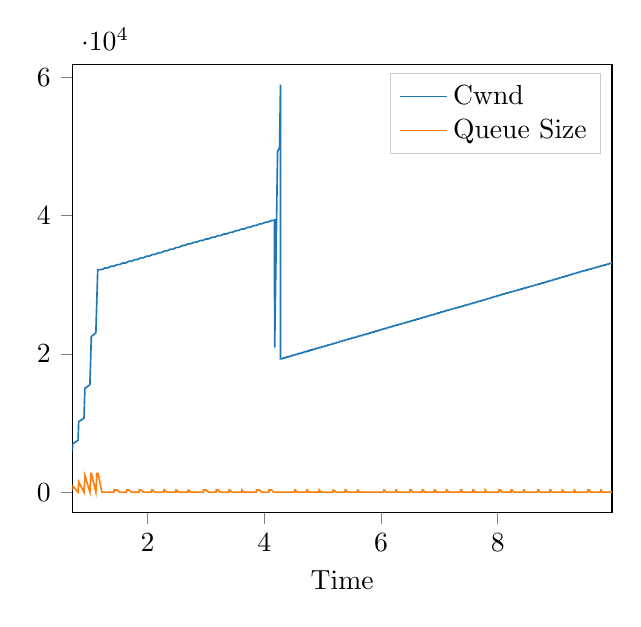
\begin{tikzpicture}

\definecolor{color0}{rgb}{0.12156862745098,0.466666666666667,0.705882352941177}
\definecolor{color1}{rgb}{1,0.498039215686275,0.0549019607843137}

\begin{axis}[
xlabel={Time},
xmin=0.712118, xmax=9.95686,
ymin=-2948, ymax=61908,
tick align=outside,
tick pos=left,
x grid style={lightgray!92.026143790849673!black},
y grid style={lightgray!92.026143790849673!black},
legend cell align={left},
legend entries={{Cwnd},{Queue Size}},
legend style={draw=white!80.0!black}
]
\addlegendimage{no markers, color0}
\addlegendimage{no markers, color1}
\addplot [semithick, color0]
table {%
0.712118 5896
0.714006 6432
0.715894 6968
0.811261 7504
0.813149 8040
0.815037 8576
0.816925 9112
0.818813 9648
0.820701 10184
0.912291 10720
0.914179 11256
0.916067 11792
0.917955 12328
0.919843 12864
0.921731 13400
0.923619 13936
0.925507 14472
0.927395 15008
1.01332 15544
1.01521 16080
1.0171 16616
1.01899 17152
1.02087 17688
1.02276 18224
1.02465 18760
1.02654 19296
1.02843 19832
1.03031 20368
1.0322 20904
1.03409 21440
1.03598 21976
1.03787 22512
1.1153 23048
1.11718 23584
1.11907 24120
1.12096 24656
1.12285 25192
1.12474 25728
1.12662 26264
1.12851 26800
1.1304 27336
1.13229 27872
1.13418 28408
1.13606 28944
1.13795 29480
1.13984 30016
1.14173 30552
1.14362 31088
1.1455 31624
1.14739 32160
1.14739 32168
1.14928 32176
1.15117 32184
1.15306 32192
1.21727 32200
1.21916 32208
1.22105 32216
1.22293 32224
1.22482 32232
1.22671 32240
1.2286 32248
1.23049 32256
1.23237 32264
1.23426 32272
1.23615 32280
1.23804 32288
1.23993 32296
1.24181 32304
1.2437 32312
1.24559 32320
1.24748 32328
1.24937 32336
1.25125 32344
1.25314 32352
1.25503 32360
1.25692 32368
1.25881 32376
1.26069 32384
1.26258 32392
1.26447 32400
1.26636 32408
1.26825 32416
1.27013 32424
1.27202 32432
1.31924 32440
1.32113 32448
1.32302 32456
1.32491 32464
1.3268 32472
1.32868 32480
1.33057 32488
1.33246 32496
1.33435 32504
1.33624 32512
1.33812 32520
1.34001 32528
1.3419 32536
1.34379 32544
1.34568 32552
1.34756 32560
1.34945 32568
1.35134 32576
1.35323 32584
1.35512 32592
1.357 32600
1.35889 32608
1.36078 32616
1.36267 32624
1.36456 32632
1.36644 32640
1.36833 32648
1.37022 32656
1.37211 32664
1.374 32672
1.42122 32680
1.42311 32688
1.425 32696
1.42688 32704
1.42877 32712
1.43066 32720
1.43255 32728
1.43444 32736
1.43632 32744
1.43821 32752
1.4401 32760
1.44199 32768
1.44388 32776
1.44576 32784
1.44765 32792
1.44954 32800
1.45143 32808
1.45332 32816
1.4552 32824
1.45709 32832
1.45898 32840
1.46087 32848
1.46276 32856
1.46464 32864
1.46653 32872
1.46842 32880
1.47031 32888
1.4722 32896
1.47408 32904
1.47597 32912
1.52319 32920
1.52508 32928
1.52697 32936
1.52886 32944
1.53075 32952
1.53263 32960
1.53452 32968
1.53641 32976
1.5383 32984
1.54019 32992
1.54207 33000
1.54396 33008
1.54585 33016
1.54774 33024
1.54963 33032
1.55151 33040
1.5534 33048
1.55529 33056
1.55718 33064
1.55907 33072
1.56095 33080
1.56284 33088
1.56473 33096
1.56662 33104
1.56851 33112
1.57039 33120
1.57228 33128
1.57417 33136
1.57606 33144
1.57795 33152
1.62422 33160
1.62611 33168
1.628 33176
1.62989 33184
1.63178 33192
1.63366 33200
1.63555 33208
1.63744 33216
1.63933 33224
1.64122 33232
1.6431 33240
1.64499 33248
1.64688 33256
1.64877 33264
1.65066 33272
1.65254 33280
1.65443 33288
1.65632 33296
1.65821 33304
1.6601 33312
1.66198 33320
1.66387 33328
1.66576 33336
1.66765 33344
1.66954 33352
1.67142 33360
1.67331 33368
1.6752 33376
1.67709 33384
1.67898 33392
1.72525 33400
1.72714 33408
1.72903 33416
1.73092 33424
1.73281 33432
1.73469 33440
1.73658 33448
1.73847 33456
1.74036 33464
1.74225 33472
1.74413 33480
1.74602 33488
1.74791 33496
1.7498 33504
1.75169 33512
1.75357 33520
1.75546 33528
1.75735 33536
1.75924 33544
1.76113 33552
1.76301 33560
1.7649 33568
1.76679 33576
1.76868 33584
1.77057 33592
1.77245 33600
1.77434 33608
1.77623 33616
1.77812 33624
1.78001 33632
1.78189 33640
1.82723 33648
1.82912 33656
1.831 33664
1.83289 33672
1.83478 33680
1.83667 33688
1.83856 33696
1.84044 33704
1.84233 33712
1.84422 33720
1.84611 33728
1.848 33736
1.84988 33744
1.85177 33752
1.85366 33760
1.85555 33768
1.85744 33776
1.85932 33784
1.86121 33792
1.8631 33800
1.86499 33808
1.86688 33816
1.86876 33824
1.87065 33832
1.87254 33840
1.87443 33848
1.87632 33856
1.8782 33864
1.88009 33872
1.88198 33880
1.88387 33888
1.9292 33896
1.93109 33904
1.93298 33912
1.93487 33920
1.93676 33928
1.93864 33936
1.94053 33944
1.94242 33952
1.94431 33960
1.9462 33968
1.94808 33976
1.94997 33984
1.95186 33992
1.95375 34000
1.95564 34008
1.95752 34016
1.95941 34024
1.9613 34032
1.96319 34040
1.96508 34048
1.96696 34056
1.96885 34064
1.97074 34072
1.97263 34080
1.97452 34088
1.9764 34096
1.97829 34104
1.98018 34112
1.98207 34120
1.98396 34128
1.98584 34136
2.03023 34144
2.03212 34152
2.03401 34160
2.0359 34168
2.03779 34176
2.03967 34184
2.04156 34192
2.04345 34200
2.04534 34208
2.04723 34216
2.04911 34224
2.051 34232
2.05289 34240
2.05478 34248
2.05667 34256
2.05855 34264
2.06044 34272
2.06233 34280
2.06422 34288
2.06611 34296
2.06799 34304
2.06988 34312
2.07177 34320
2.07366 34328
2.07555 34336
2.07743 34344
2.07932 34352
2.08121 34360
2.0831 34368
2.08499 34376
2.08687 34384
2.13126 34392
2.13315 34400
2.13504 34408
2.13693 34416
2.13882 34424
2.1407 34432
2.14259 34440
2.14448 34448
2.14637 34456
2.14826 34464
2.15014 34472
2.15203 34480
2.15392 34488
2.15581 34496
2.1577 34504
2.15958 34512
2.16147 34520
2.16336 34528
2.16525 34536
2.16714 34544
2.16902 34552
2.17091 34560
2.1728 34568
2.17469 34576
2.17658 34584
2.17846 34592
2.18035 34600
2.18224 34608
2.18413 34616
2.18602 34624
2.1879 34632
2.18979 34640
2.23324 34648
2.23513 34656
2.23701 34664
2.2389 34672
2.24079 34680
2.24268 34688
2.24457 34696
2.24645 34704
2.24834 34712
2.25023 34720
2.25212 34728
2.25401 34736
2.25589 34744
2.25778 34752
2.25967 34760
2.26156 34768
2.26345 34776
2.26533 34784
2.26722 34792
2.26911 34800
2.271 34808
2.27289 34816
2.27477 34824
2.27666 34832
2.27855 34840
2.28044 34848
2.28233 34856
2.28421 34864
2.2861 34872
2.28799 34880
2.28988 34888
2.29177 34896
2.33521 34904
2.3371 34912
2.33899 34920
2.34088 34928
2.34276 34936
2.34465 34944
2.34654 34952
2.34843 34960
2.35032 34968
2.3522 34976
2.35409 34984
2.35598 34992
2.35787 35000
2.35976 35008
2.36164 35016
2.36353 35024
2.36542 35032
2.36731 35040
2.3692 35048
2.37108 35056
2.37297 35064
2.37486 35072
2.37675 35080
2.37864 35088
2.38052 35096
2.38241 35104
2.3843 35112
2.38619 35120
2.38808 35128
2.38996 35136
2.39185 35144
2.39374 35152
2.43624 35160
2.43813 35168
2.44002 35176
2.44191 35184
2.4438 35192
2.44568 35200
2.44757 35208
2.44946 35216
2.45135 35224
2.45324 35232
2.45512 35240
2.45701 35248
2.4589 35256
2.46079 35264
2.46268 35272
2.46456 35280
2.46645 35288
2.46834 35296
2.47023 35304
2.47212 35312
2.474 35320
2.47589 35328
2.47778 35336
2.47967 35344
2.48156 35352
2.48344 35360
2.48533 35368
2.48722 35376
2.48911 35384
2.491 35392
2.49288 35400
2.49477 35408
2.53727 35416
2.53916 35424
2.54105 35432
2.54294 35440
2.54483 35448
2.54671 35456
2.5486 35464
2.55049 35472
2.55238 35480
2.55427 35488
2.55615 35496
2.55804 35504
2.55993 35512
2.56182 35520
2.56371 35528
2.56559 35536
2.56748 35544
2.56937 35552
2.57126 35560
2.57315 35568
2.57503 35576
2.57692 35584
2.57881 35592
2.5807 35600
2.58259 35608
2.58447 35616
2.58636 35624
2.58825 35632
2.59014 35640
2.59203 35648
2.59391 35656
2.5958 35664
2.59769 35672
2.63925 35680
2.64114 35688
2.64302 35696
2.64491 35704
2.6468 35712
2.64869 35720
2.65058 35728
2.65246 35736
2.65435 35744
2.65624 35752
2.65813 35760
2.66002 35768
2.6619 35776
2.66379 35784
2.66568 35792
2.66757 35800
2.66946 35808
2.67134 35816
2.67323 35824
2.67512 35832
2.67701 35840
2.6789 35848
2.68078 35856
2.68267 35864
2.68456 35872
2.68645 35880
2.68834 35888
2.69022 35896
2.69211 35904
2.694 35912
2.69589 35920
2.69778 35927
2.69966 35934
2.74122 35941
2.74311 35948
2.745 35955
2.74689 35962
2.74877 35969
2.75066 35976
2.75255 35983
2.75444 35990
2.75633 35997
2.75821 36004
2.7601 36011
2.76199 36018
2.76388 36025
2.76577 36032
2.76765 36039
2.76954 36046
2.77143 36053
2.77332 36060
2.77521 36067
2.77709 36074
2.77898 36081
2.78087 36088
2.78276 36095
2.78465 36102
2.78653 36109
2.78842 36116
2.79031 36123
2.7922 36130
2.79409 36137
2.79597 36144
2.79786 36151
2.79975 36158
2.80164 36165
2.84225 36172
2.84414 36179
2.84603 36186
2.84792 36193
2.8498 36200
2.85169 36207
2.85358 36214
2.85547 36221
2.85736 36228
2.85924 36235
2.86113 36242
2.86302 36249
2.86491 36256
2.8668 36263
2.86868 36270
2.87057 36277
2.87246 36284
2.87435 36291
2.87624 36298
2.87812 36305
2.88001 36312
2.8819 36319
2.88379 36326
2.88568 36333
2.88756 36340
2.88945 36347
2.89134 36354
2.89323 36361
2.89512 36368
2.897 36375
2.89889 36382
2.90078 36389
2.90267 36396
2.94328 36403
2.94517 36410
2.94706 36417
2.94895 36424
2.95084 36431
2.95272 36438
2.95461 36445
2.9565 36452
2.95839 36459
2.96028 36466
2.96216 36473
2.96405 36480
2.96594 36487
2.96783 36494
2.96972 36501
2.9716 36508
2.97349 36515
2.97538 36522
2.97727 36529
2.97916 36536
2.98104 36543
2.98293 36550
2.98482 36557
2.98671 36564
2.9886 36571
2.99048 36578
2.99237 36585
2.99426 36592
2.99615 36599
2.99804 36606
2.99992 36613
3.00181 36620
3.0037 36627
3.04431 36634
3.0462 36641
3.04809 36648
3.04998 36655
3.05187 36662
3.05375 36669
3.05564 36676
3.05753 36683
3.05942 36690
3.06131 36697
3.06319 36704
3.06508 36711
3.06697 36718
3.06886 36725
3.07075 36732
3.07263 36739
3.07452 36746
3.07641 36753
3.0783 36760
3.08019 36767
3.08207 36774
3.08396 36781
3.08585 36788
3.08774 36795
3.08963 36802
3.09151 36809
3.0934 36816
3.09529 36823
3.09718 36830
3.09907 36837
3.10095 36844
3.10284 36851
3.10473 36858
3.10662 36865
3.14629 36872
3.14818 36879
3.15006 36886
3.15195 36893
3.15384 36900
3.15573 36907
3.15762 36914
3.1595 36921
3.16139 36928
3.16328 36935
3.16517 36942
3.16706 36949
3.16894 36956
3.17083 36963
3.17272 36970
3.17461 36977
3.1765 36984
3.17838 36991
3.18027 36998
3.18216 37005
3.18405 37012
3.18594 37019
3.18782 37026
3.18971 37033
3.1916 37040
3.19349 37047
3.19538 37054
3.19726 37061
3.19915 37068
3.20104 37075
3.20293 37082
3.20482 37089
3.2067 37096
3.20859 37103
3.24826 37110
3.25015 37117
3.25204 37124
3.25393 37131
3.25581 37138
3.2577 37145
3.25959 37152
3.26148 37159
3.26337 37166
3.26525 37173
3.26714 37180
3.26903 37187
3.27092 37194
3.27281 37201
3.27469 37208
3.27658 37215
3.27847 37222
3.28036 37229
3.28225 37236
3.28413 37243
3.28602 37250
3.28791 37257
3.2898 37264
3.29169 37271
3.29357 37278
3.29546 37285
3.29735 37292
3.29924 37299
3.30113 37306
3.30301 37313
3.3049 37320
3.30679 37327
3.30868 37334
3.31057 37341
3.34929 37348
3.35118 37355
3.35307 37362
3.35496 37369
3.35684 37376
3.35873 37383
3.36062 37390
3.36251 37397
3.3644 37404
3.36628 37411
3.36817 37418
3.37006 37425
3.37195 37432
3.37384 37439
3.37572 37446
3.37761 37453
3.3795 37460
3.38139 37467
3.38328 37474
3.38516 37481
3.38705 37488
3.38894 37495
3.39083 37502
3.39272 37509
3.3946 37516
3.39649 37523
3.39838 37530
3.40027 37537
3.40216 37544
3.40404 37551
3.40593 37558
3.40782 37565
3.40971 37572
3.4116 37579
3.45032 37586
3.45221 37593
3.4541 37600
3.45599 37607
3.45788 37614
3.45976 37621
3.46165 37628
3.46354 37635
3.46543 37642
3.46732 37649
3.4692 37656
3.47109 37663
3.47298 37670
3.47487 37677
3.47676 37684
3.47864 37691
3.48053 37698
3.48242 37705
3.48431 37712
3.4862 37719
3.48808 37726
3.48997 37733
3.49186 37740
3.49375 37747
3.49564 37754
3.49752 37761
3.49941 37768
3.5013 37775
3.50319 37782
3.50508 37789
3.50696 37796
3.50885 37803
3.51074 37810
3.51263 37817
3.51452 37824
3.5523 37831
3.55419 37838
3.55607 37845
3.55796 37852
3.55985 37859
3.56174 37866
3.56363 37873
3.56551 37880
3.5674 37887
3.56929 37894
3.57118 37901
3.57307 37908
3.57495 37915
3.57684 37922
3.57873 37929
3.58062 37936
3.58251 37943
3.58439 37950
3.58628 37957
3.58817 37964
3.59006 37971
3.59195 37978
3.59383 37985
3.59572 37992
3.59761 37999
3.5995 38006
3.60139 38013
3.60327 38020
3.60516 38027
3.60705 38034
3.60894 38041
3.61083 38048
3.61271 38055
3.6146 38062
3.61649 38069
3.65427 38076
3.65616 38083
3.65805 38090
3.65994 38097
3.66182 38104
3.66371 38111
3.6656 38118
3.66749 38125
3.66938 38132
3.67126 38139
3.67315 38146
3.67504 38153
3.67693 38160
3.67882 38167
3.6807 38174
3.68259 38181
3.68448 38188
3.68637 38195
3.68826 38202
3.69014 38209
3.69203 38216
3.69392 38223
3.69581 38230
3.6977 38237
3.69958 38244
3.70147 38251
3.70336 38258
3.70525 38265
3.70714 38272
3.70902 38279
3.71091 38286
3.7128 38293
3.71469 38300
3.71658 38307
3.71846 38314
3.7553 38321
3.75719 38328
3.75908 38335
3.76097 38342
3.76285 38349
3.76474 38356
3.76663 38363
3.76852 38370
3.77041 38377
3.77229 38384
3.77418 38391
3.77607 38398
3.77796 38405
3.77985 38412
3.78173 38419
3.78362 38426
3.78551 38433
3.7874 38440
3.78929 38447
3.79117 38454
3.79306 38461
3.79495 38468
3.79684 38475
3.79873 38482
3.80061 38489
3.8025 38496
3.80439 38503
3.80628 38510
3.80817 38517
3.81005 38524
3.81194 38531
3.81383 38538
3.81572 38545
3.81761 38552
3.81949 38559
3.85633 38566
3.85822 38573
3.86011 38580
3.862 38587
3.86388 38594
3.86577 38601
3.86766 38608
3.86955 38615
3.87144 38622
3.87332 38629
3.87521 38636
3.8771 38643
3.87899 38650
3.88088 38657
3.88276 38664
3.88465 38671
3.88654 38678
3.88843 38685
3.89032 38692
3.8922 38699
3.89409 38706
3.89598 38713
3.89787 38720
3.89976 38727
3.90164 38734
3.90353 38741
3.90542 38748
3.90731 38755
3.9092 38762
3.91108 38769
3.91297 38776
3.91486 38783
3.91675 38790
3.91864 38797
3.92052 38804
3.95736 38811
3.95925 38818
3.96114 38825
3.96303 38832
3.96492 38839
3.9668 38846
3.96869 38853
3.97058 38860
3.97247 38867
3.97436 38874
3.97624 38881
3.97813 38888
3.98002 38895
3.98191 38902
3.9838 38909
3.98568 38916
3.98757 38923
3.98946 38930
3.99135 38937
3.99324 38944
3.99512 38951
3.99701 38958
3.9989 38965
4.00079 38972
4.00268 38979
4.00456 38986
4.00645 38993
4.00834 39000
4.01023 39007
4.01212 39014
4.014 39021
4.01589 39028
4.01778 39035
4.01967 39042
4.02156 39049
4.02344 39056
4.05934 39063
4.06123 39070
4.06311 39077
4.065 39084
4.06689 39091
4.06878 39098
4.07067 39105
4.07255 39112
4.07444 39119
4.07633 39126
4.07822 39133
4.08011 39140
4.08199 39147
4.08388 39154
4.08577 39161
4.08766 39168
4.08955 39175
4.09143 39182
4.09332 39189
4.09521 39196
4.0971 39203
4.09899 39210
4.10087 39217
4.10276 39224
4.10465 39231
4.10654 39238
4.10843 39245
4.11031 39252
4.1122 39259
4.11409 39266
4.11598 39273
4.11787 39280
4.11975 39287
4.12164 39294
4.12353 39301
4.12542 39308
4.16131 39315
4.1632 39322
4.16509 39329
4.16698 39336
4.16886 39343
4.17075 39350
4.17264 39357
4.17453 39364
4.1783 20904
4.17925 21440
4.18019 21976
4.18114 22512
4.18208 23048
4.18302 23584
4.18397 24120
4.18491 24656
4.18586 25192
4.1868 25728
4.18774 26264
4.18869 26800
4.18963 27336
4.19058 27872
4.19152 28408
4.19246 28944
4.19341 29480
4.19435 30016
4.1953 30552
4.19624 31088
4.19718 31624
4.19813 32160
4.19907 32696
4.20002 33232
4.20096 33768
4.2019 34304
4.20285 34840
4.20379 35376
4.20474 35912
4.20568 36448
4.20662 36984
4.20757 37520
4.20851 38056
4.20946 38592
4.2104 39128
4.21134 39664
4.21229 40200
4.21323 40736
4.21418 41272
4.21512 41808
4.21606 42344
4.21701 42880
4.21795 43416
4.2189 43952
4.21984 44488
4.22078 45024
4.22173 45560
4.22267 46096
4.22362 46632
4.22456 47168
4.2255 47704
4.22645 48240
4.22739 48776
4.22834 49312
4.26234 49848
4.26329 50384
4.26423 50920
4.26517 51456
4.26612 51992
4.26706 52528
4.26801 53064
4.26895 53600
4.26989 54136
4.27084 54672
4.27178 55208
4.27273 55744
4.27367 56280
4.27461 56816
4.27556 57352
4.2765 57888
4.27745 58424
4.27839 58960
4.27933 19296
4.31521 19310
4.31709 19324
4.31898 19338
4.32087 19352
4.32276 19366
4.32465 19380
4.32653 19394
4.32842 19408
4.36337 19422
4.36526 19436
4.36715 19450
4.36904 19464
4.37092 19478
4.37281 19492
4.3747 19506
4.37659 19520
4.37848 19534
4.38036 19548
4.41718 19562
4.41907 19576
4.42096 19590
4.42284 19604
4.42473 19618
4.42662 19632
4.42851 19646
4.4304 19660
4.46535 19674
4.46724 19688
4.46912 19702
4.47101 19716
4.4729 19730
4.47479 19744
4.47668 19758
4.47856 19772
4.48045 19786
4.48234 19800
4.51916 19814
4.52104 19828
4.52293 19842
4.52482 19856
4.52671 19870
4.5286 19884
4.53048 19898
4.53237 19912
4.56732 19926
4.56921 19940
4.5711 19954
4.57299 19968
4.57487 19982
4.57676 19996
4.57865 20010
4.58054 20024
4.58243 20038
4.58431 20052
4.62113 20066
4.62302 20080
4.62491 20094
4.62679 20108
4.62868 20122
4.63057 20136
4.63246 20150
4.63435 20164
4.66835 20178
4.67024 20192
4.67213 20206
4.67402 20220
4.6759 20234
4.67779 20248
4.67968 20262
4.68157 20276
4.68346 20290
4.68534 20304
4.72216 20318
4.72405 20332
4.72594 20346
4.72782 20360
4.72971 20374
4.7316 20388
4.73349 20402
4.73538 20416
4.76938 20430
4.77127 20444
4.77316 20458
4.77505 20472
4.77693 20486
4.77882 20500
4.78071 20514
4.7826 20528
4.78449 20541
4.78637 20554
4.82319 20567
4.82508 20580
4.82697 20593
4.82885 20606
4.83074 20619
4.83263 20632
4.83452 20645
4.83641 20658
4.83829 20671
4.87136 20684
4.87324 20697
4.87513 20710
4.87702 20723
4.87891 20736
4.8808 20749
4.88268 20762
4.88457 20775
4.88646 20788
4.88835 20801
4.92516 20814
4.92705 20827
4.92894 20840
4.93083 20853
4.93272 20866
4.9346 20879
4.93649 20892
4.93838 20905
4.94027 20918
4.97333 20931
4.97522 20944
4.97711 20957
4.979 20970
4.98088 20983
4.98277 20996
4.98466 21009
4.98655 21022
4.98844 21035
4.99032 21048
5.02714 21061
5.02903 21074
5.03092 21087
5.0328 21100
5.03469 21113
5.03658 21126
5.03847 21139
5.04036 21152
5.04224 21165
5.07436 21178
5.07625 21191
5.07814 21204
5.08003 21217
5.08191 21230
5.0838 21243
5.08569 21256
5.08758 21269
5.08947 21282
5.09135 21295
5.12817 21308
5.13006 21321
5.13195 21334
5.13383 21347
5.13572 21360
5.13761 21373
5.1395 21386
5.14139 21399
5.14327 21412
5.17539 21425
5.17728 21438
5.17917 21451
5.18106 21464
5.18294 21477
5.18483 21490
5.18672 21503
5.18861 21516
5.1905 21529
5.19238 21542
5.2292 21555
5.23109 21568
5.23298 21581
5.23486 21594
5.23675 21607
5.23864 21620
5.24053 21633
5.24242 21646
5.2443 21659
5.27642 21672
5.27831 21685
5.2802 21698
5.28209 21711
5.28397 21724
5.28586 21737
5.28775 21750
5.28964 21763
5.29153 21776
5.29341 21789
5.2953 21802
5.33117 21815
5.33306 21828
5.33495 21841
5.33684 21854
5.33873 21867
5.34061 21880
5.3425 21893
5.34439 21906
5.34628 21919
5.3784 21932
5.38028 21945
5.38217 21958
5.38406 21971
5.38595 21984
5.38784 21997
5.38972 22010
5.39161 22023
5.3935 22036
5.39539 22049
5.39728 22062
5.43315 22075
5.43504 22088
5.43692 22101
5.43881 22113
5.4407 22125
5.44259 22137
5.44448 22149
5.44636 22161
5.44825 22173
5.48037 22185
5.48226 22197
5.48415 22209
5.48604 22221
5.48792 22233
5.48981 22245
5.4917 22257
5.49359 22269
5.49548 22281
5.49736 22293
5.49925 22305
5.53418 22317
5.53607 22329
5.53796 22341
5.53984 22353
5.54173 22365
5.54362 22377
5.54551 22389
5.5474 22401
5.54928 22413
5.5814 22425
5.58329 22437
5.58518 22449
5.58707 22461
5.58895 22473
5.59084 22485
5.59273 22497
5.59462 22509
5.59651 22521
5.59839 22533
5.60028 22545
5.63521 22557
5.6371 22569
5.63899 22581
5.64087 22593
5.64276 22605
5.64465 22617
5.64654 22629
5.64843 22641
5.65031 22653
5.68243 22665
5.68432 22677
5.68621 22689
5.6881 22701
5.68998 22713
5.69187 22725
5.69376 22737
5.69565 22749
5.69754 22761
5.69942 22773
5.70131 22785
5.7032 22797
5.73718 22809
5.73907 22821
5.74096 22833
5.74285 22845
5.74474 22857
5.74662 22869
5.74851 22881
5.7504 22893
5.75229 22905
5.78441 22917
5.78629 22929
5.78818 22941
5.79007 22953
5.79196 22965
5.79385 22977
5.79573 22989
5.79762 23001
5.79951 23013
5.8014 23025
5.80329 23037
5.80517 23049
5.83916 23061
5.84105 23073
5.84293 23085
5.84482 23097
5.84671 23109
5.8486 23121
5.85049 23133
5.85237 23145
5.85426 23157
5.88638 23169
5.88827 23181
5.89016 23193
5.89204 23205
5.89393 23217
5.89582 23229
5.89771 23241
5.8996 23253
5.90148 23265
5.90337 23277
5.90526 23289
5.90715 23301
5.94019 23313
5.94208 23325
5.94396 23337
5.94585 23349
5.94774 23361
5.94963 23373
5.95152 23385
5.9534 23397
5.95529 23409
5.98741 23421
5.9893 23433
5.99119 23445
5.99308 23457
5.99496 23469
5.99685 23481
5.99874 23493
6.00063 23505
6.00252 23517
6.0044 23529
6.00629 23541
6.00818 23553
6.04122 23565
6.04311 23577
6.045 23589
6.04688 23601
6.04877 23613
6.05066 23625
6.05255 23637
6.05444 23649
6.05632 23661
6.08844 23673
6.09033 23685
6.09222 23697
6.09411 23709
6.09599 23721
6.09788 23733
6.09977 23745
6.10166 23757
6.10355 23769
6.10543 23781
6.10732 23793
6.10921 23805
6.14225 23817
6.14414 23829
6.14603 23841
6.14791 23853
6.1498 23865
6.15169 23877
6.15358 23889
6.15547 23901
6.15735 23913
6.15924 23925
6.19042 23937
6.1923 23949
6.19419 23960
6.19608 23971
6.19797 23982
6.19986 23993
6.20174 24004
6.20363 24015
6.20552 24026
6.20741 24037
6.2093 24048
6.21118 24059
6.24422 24070
6.24611 24081
6.248 24092
6.24989 24103
6.25178 24114
6.25366 24125
6.25555 24136
6.25744 24147
6.25933 24158
6.26122 24169
6.29239 24180
6.29428 24191
6.29617 24202
6.29805 24213
6.29994 24224
6.30183 24235
6.30372 24246
6.30561 24257
6.30749 24268
6.30938 24279
6.31127 24290
6.31316 24301
6.3462 24312
6.34809 24323
6.34997 24334
6.35186 24345
6.35375 24356
6.35564 24367
6.35753 24378
6.35941 24389
6.3613 24400
6.36319 24411
6.39342 24422
6.39531 24433
6.3972 24444
6.39908 24455
6.40097 24466
6.40286 24477
6.40475 24488
6.40664 24499
6.40852 24510
6.41041 24521
6.4123 24532
6.41419 24543
6.44723 24554
6.44912 24565
6.451 24576
6.45289 24587
6.45478 24598
6.45667 24609
6.45856 24620
6.46044 24631
6.46233 24642
6.46422 24653
6.49445 24664
6.49634 24675
6.49823 24686
6.50012 24697
6.502 24708
6.50389 24719
6.50578 24730
6.50767 24741
6.50956 24752
6.51144 24763
6.51333 24774
6.51522 24785
6.54826 24796
6.55015 24807
6.55204 24818
6.55392 24829
6.55581 24840
6.5577 24851
6.55959 24862
6.56148 24873
6.56336 24884
6.56525 24895
6.59548 24906
6.59737 24917
6.59926 24928
6.60115 24939
6.60303 24950
6.60492 24961
6.60681 24972
6.6087 24983
6.61059 24994
6.61247 25005
6.61436 25016
6.61625 25027
6.61814 25038
6.65023 25049
6.65212 25060
6.65401 25071
6.6559 25082
6.65779 25093
6.65967 25104
6.66156 25115
6.66345 25126
6.66534 25137
6.66723 25148
6.69746 25159
6.69934 25170
6.70123 25181
6.70312 25192
6.70501 25203
6.7069 25214
6.70878 25225
6.71067 25236
6.71256 25247
6.71445 25258
6.71634 25269
6.71822 25280
6.72011 25291
6.75221 25302
6.7541 25313
6.75598 25324
6.75787 25335
6.75976 25346
6.76165 25357
6.76354 25368
6.76542 25379
6.76731 25390
6.7692 25401
6.79943 25412
6.80132 25423
6.80321 25434
6.80509 25445
6.80698 25456
6.80887 25467
6.81076 25478
6.81265 25489
6.81453 25500
6.81642 25511
6.81831 25522
6.8202 25533
6.82209 25544
6.85324 25555
6.85513 25566
6.85701 25577
6.8589 25588
6.86079 25599
6.86268 25610
6.86457 25621
6.86645 25632
6.86834 25643
6.87023 25654
6.90046 25665
6.90235 25676
6.90424 25687
6.90612 25698
6.90801 25709
6.9099 25720
6.91179 25731
6.91368 25742
6.91556 25753
6.91745 25764
6.91934 25775
6.92123 25786
6.92312 25797
6.95427 25808
6.95616 25819
6.95804 25830
6.95993 25841
6.96182 25852
6.96371 25863
6.9656 25874
6.96748 25885
6.96937 25896
6.97126 25907
7.00149 25918
7.00338 25929
7.00527 25940
7.00716 25951
7.00904 25962
7.01093 25973
7.01282 25984
7.01471 25995
7.0166 26006
7.01848 26017
7.02037 26028
7.02226 26039
7.02415 26050
7.02604 26061
7.05624 26072
7.05813 26083
7.06002 26094
7.06191 26105
7.0638 26116
7.06568 26127
7.06757 26137
7.06946 26147
7.07135 26157
7.07324 26167
7.10347 26177
7.10535 26187
7.10724 26197
7.10913 26207
7.11102 26217
7.11291 26227
7.11479 26237
7.11668 26247
7.11857 26257
7.12046 26267
7.12235 26277
7.12423 26287
7.12612 26297
7.12801 26307
7.15822 26317
7.16011 26327
7.16199 26337
7.16388 26347
7.16577 26357
7.16766 26367
7.16955 26377
7.17143 26387
7.17332 26397
7.17521 26407
7.20544 26417
7.20733 26427
7.20922 26437
7.2111 26447
7.21299 26457
7.21488 26467
7.21677 26477
7.21866 26487
7.22054 26497
7.22243 26507
7.22432 26517
7.22621 26527
7.2281 26537
7.22998 26547
7.25925 26557
7.26114 26567
7.26302 26577
7.26491 26587
7.2668 26597
7.26869 26607
7.27058 26617
7.27246 26627
7.27435 26637
7.27624 26647
7.30647 26657
7.30836 26667
7.31025 26677
7.31213 26687
7.31402 26697
7.31591 26707
7.3178 26717
7.31969 26727
7.32157 26737
7.32346 26747
7.32535 26757
7.32724 26767
7.32913 26777
7.33101 26787
7.36028 26797
7.36217 26807
7.36405 26817
7.36594 26827
7.36783 26837
7.36972 26847
7.37161 26857
7.37349 26867
7.37538 26877
7.37727 26887
7.4075 26897
7.40939 26907
7.41128 26917
7.41316 26927
7.41505 26937
7.41694 26947
7.41883 26957
7.42072 26967
7.4226 26977
7.42449 26987
7.42638 26997
7.42827 27007
7.43016 27017
7.43204 27027
7.46131 27037
7.4632 27047
7.46508 27057
7.46697 27067
7.46886 27077
7.47075 27087
7.47264 27097
7.47452 27107
7.47641 27117
7.4783 27127
7.48019 27137
7.50948 27147
7.51136 27157
7.51325 27167
7.51514 27177
7.51703 27187
7.51892 27197
7.5208 27207
7.52269 27217
7.52458 27227
7.52647 27237
7.52836 27247
7.53024 27257
7.53213 27267
7.53402 27277
7.56328 27287
7.56517 27297
7.56706 27307
7.56895 27317
7.57084 27327
7.57272 27337
7.57461 27347
7.5765 27357
7.57839 27367
7.58028 27377
7.58216 27387
7.61145 27397
7.61334 27407
7.61523 27417
7.61711 27427
7.619 27437
7.62089 27447
7.62278 27457
7.62467 27467
7.62655 27477
7.62844 27487
7.63033 27497
7.63222 27507
7.63411 27517
7.63599 27527
7.66526 27537
7.66715 27547
7.66903 27557
7.67092 27567
7.67281 27577
7.6747 27587
7.67659 27597
7.67847 27607
7.68036 27617
7.68225 27627
7.68414 27637
7.71248 27647
7.71437 27657
7.71626 27667
7.71814 27677
7.72003 27687
7.72192 27697
7.72381 27707
7.7257 27717
7.72758 27727
7.72947 27737
7.73136 27747
7.73325 27757
7.73514 27767
7.73702 27777
7.76629 27787
7.76818 27797
7.77006 27807
7.77195 27817
7.77384 27827
7.77573 27837
7.77762 27847
7.7795 27857
7.78139 27867
7.78328 27877
7.78517 27887
7.81351 27897
7.8154 27907
7.81729 27917
7.81917 27927
7.82106 27937
7.82295 27947
7.82484 27957
7.82673 27967
7.82861 27977
7.8305 27987
7.83239 27997
7.83428 28007
7.83617 28017
7.83805 28027
7.86732 28037
7.86921 28047
7.87109 28057
7.87298 28067
7.87487 28077
7.87676 28087
7.87865 28097
7.88053 28107
7.88242 28117
7.88431 28127
7.8862 28137
7.88809 28147
7.91548 28157
7.91737 28167
7.91926 28177
7.92115 28187
7.92304 28197
7.92492 28207
7.92681 28217
7.9287 28227
7.93059 28237
7.93248 28247
7.93436 28257
7.93625 28267
7.93814 28277
7.94003 28287
7.96929 28297
7.97118 28307
7.97307 28317
7.97496 28327
7.97684 28337
7.97873 28347
7.98062 28357
7.98251 28367
7.9844 28377
7.98628 28387
7.98817 28397
7.99006 28407
8.01746 28417
8.01935 28427
8.02124 28437
8.02312 28447
8.02501 28457
8.0269 28467
8.02879 28477
8.03068 28487
8.03256 28497
8.03445 28507
8.03634 28517
8.03823 28527
8.04012 28537
8.042 28547
8.07127 28557
8.07316 28567
8.07504 28577
8.07693 28587
8.07882 28597
8.08071 28607
8.0826 28617
8.08448 28627
8.08637 28637
8.08826 28647
8.09015 28657
8.09204 28667
8.11943 28677
8.12132 28687
8.12321 28697
8.1251 28707
8.12699 28717
8.12887 28727
8.13076 28737
8.13265 28746
8.13454 28755
8.13643 28764
8.13831 28773
8.1402 28782
8.14209 28791
8.14398 28800
8.1723 28809
8.17419 28818
8.17607 28827
8.17796 28836
8.17985 28845
8.18174 28854
8.18363 28863
8.18551 28872
8.1874 28881
8.18929 28890
8.19118 28899
8.19307 28908
8.22046 28917
8.22235 28926
8.22424 28935
8.22613 28944
8.22802 28953
8.2299 28962
8.23179 28971
8.23368 28980
8.23557 28989
8.23746 28998
8.23934 29007
8.24123 29016
8.24312 29025
8.24501 29034
8.27333 29043
8.27522 29052
8.2771 29061
8.27899 29070
8.28088 29079
8.28277 29088
8.28466 29097
8.28654 29106
8.28843 29115
8.29032 29124
8.29221 29133
8.2941 29142
8.32149 29151
8.32338 29160
8.32527 29169
8.32716 29178
8.32905 29187
8.33093 29196
8.33282 29205
8.33471 29214
8.3366 29223
8.33849 29232
8.34037 29241
8.34226 29250
8.34415 29259
8.34604 29268
8.34793 29277
8.3753 29286
8.37719 29295
8.37908 29304
8.38097 29313
8.38285 29322
8.38474 29331
8.38663 29340
8.38852 29349
8.39041 29358
8.39229 29367
8.39418 29376
8.39607 29385
8.42347 29394
8.42536 29403
8.42724 29412
8.42913 29421
8.43102 29430
8.43291 29439
8.4348 29448
8.43668 29457
8.43857 29466
8.44046 29475
8.44235 29484
8.44424 29493
8.44612 29502
8.44801 29511
8.4499 29520
8.47728 29529
8.47916 29538
8.48105 29547
8.48294 29556
8.48483 29565
8.48672 29574
8.4886 29583
8.49049 29592
8.49238 29601
8.49427 29610
8.49616 29619
8.49804 29628
8.52544 29637
8.52733 29646
8.52922 29655
8.53111 29664
8.533 29673
8.53488 29682
8.53677 29691
8.53866 29700
8.54055 29709
8.54244 29718
8.54432 29727
8.54621 29736
8.5481 29745
8.54999 29754
8.55188 29763
8.57831 29772
8.5802 29781
8.58208 29790
8.58397 29799
8.58586 29808
8.58775 29817
8.58964 29826
8.59152 29835
8.59341 29844
8.5953 29853
8.59719 29862
8.59907 29871
8.62647 29880
8.62836 29889
8.63025 29898
8.63214 29907
8.63403 29916
8.63591 29925
8.6378 29934
8.63969 29943
8.64158 29952
8.64347 29961
8.64535 29970
8.64724 29979
8.64913 29988
8.65102 29997
8.65291 30006
8.67934 30015
8.68123 30024
8.68311 30033
8.685 30042
8.68689 30051
8.68878 30060
8.69067 30069
8.69255 30078
8.69444 30087
8.69633 30096
8.69822 30105
8.70011 30114
8.7275 30123
8.72939 30132
8.73128 30141
8.73317 30150
8.73506 30159
8.73694 30168
8.73883 30177
8.74072 30186
8.74261 30195
8.7445 30204
8.74638 30213
8.74827 30222
8.75016 30231
8.75205 30240
8.75394 30249
8.78037 30258
8.78226 30267
8.78414 30276
8.78603 30285
8.78792 30294
8.78981 30303
8.7917 30312
8.79358 30321
8.79547 30330
8.79736 30339
8.79925 30348
8.80114 30357
8.80302 30366
8.82948 30375
8.83137 30384
8.83325 30393
8.83514 30402
8.83703 30411
8.83892 30420
8.84081 30429
8.84269 30438
8.84458 30447
8.84647 30456
8.84836 30465
8.85025 30474
8.85213 30483
8.85402 30492
8.85591 30501
8.88234 30510
8.88423 30519
8.88612 30528
8.88801 30537
8.88989 30546
8.89178 30555
8.89367 30564
8.89556 30573
8.89745 30582
8.89933 30591
8.90122 30600
8.90311 30609
8.905 30618
8.93145 30627
8.93334 30636
8.93523 30645
8.93712 30654
8.939 30663
8.94089 30672
8.94278 30681
8.94467 30690
8.94656 30699
8.94844 30708
8.95033 30717
8.95222 30726
8.95411 30735
8.956 30744
8.95788 30753
8.98432 30762
8.9862 30771
8.98809 30780
8.98998 30789
8.99187 30798
8.99376 30807
8.99564 30816
8.99753 30825
8.99942 30834
9.00131 30843
9.0032 30852
9.00508 30861
9.00697 30870
9.03248 30879
9.03437 30888
9.03626 30897
9.03815 30906
9.04004 30915
9.04192 30924
9.04381 30933
9.0457 30942
9.04759 30951
9.04948 30960
9.05136 30969
9.05325 30978
9.05514 30987
9.05703 30996
9.05892 31005
9.08535 31014
9.08724 31023
9.08912 31032
9.09101 31041
9.0929 31050
9.09479 31059
9.09667 31068
9.09856 31077
9.10045 31086
9.10234 31095
9.10423 31104
9.10611 31113
9.108 31122
9.13351 31131
9.1354 31140
9.13729 31149
9.13918 31158
9.14107 31167
9.14295 31176
9.14484 31185
9.14673 31194
9.14862 31203
9.15051 31212
9.15239 31221
9.15428 31230
9.15617 31239
9.15806 31248
9.15995 31257
9.18638 31266
9.18827 31275
9.19015 31284
9.19204 31293
9.19393 31302
9.19582 31311
9.19771 31320
9.19959 31329
9.20148 31338
9.20337 31347
9.20526 31356
9.20715 31365
9.20903 31374
9.21092 31383
9.23549 31392
9.23738 31401
9.23926 31410
9.24115 31419
9.24304 31428
9.24493 31437
9.24682 31446
9.2487 31455
9.25059 31464
9.25248 31473
9.25437 31482
9.25626 31491
9.25814 31500
9.26003 31509
9.26192 31518
9.28835 31527
9.29024 31536
9.29213 31545
9.29402 31554
9.2959 31563
9.29779 31572
9.29968 31581
9.30157 31590
9.30346 31599
9.30534 31608
9.30723 31617
9.30912 31626
9.31101 31635
9.3129 31644
9.33746 31653
9.33935 31662
9.34124 31671
9.34313 31680
9.34501 31689
9.3469 31698
9.34879 31707
9.35068 31716
9.35257 31725
9.35445 31734
9.35634 31743
9.35823 31752
9.36012 31761
9.36201 31770
9.36389 31779
9.39033 31788
9.39221 31797
9.3941 31806
9.39599 31815
9.39788 31824
9.39977 31833
9.40165 31842
9.40354 31851
9.40543 31860
9.40732 31869
9.40921 31878
9.41109 31887
9.41298 31896
9.41487 31905
9.43849 31914
9.44038 31923
9.44227 31931
9.44416 31939
9.44604 31947
9.44793 31955
9.44982 31963
9.45171 31971
9.4536 31979
9.45548 31987
9.45737 31995
9.45926 32003
9.46115 32011
9.46304 32019
9.46492 32027
9.49136 32035
9.49324 32043
9.49513 32051
9.49702 32059
9.49891 32067
9.5008 32075
9.50268 32083
9.50457 32091
9.50646 32099
9.50835 32107
9.51024 32115
9.51212 32123
9.51401 32131
9.5159 32139
9.53952 32147
9.54141 32155
9.5433 32163
9.54519 32171
9.54708 32179
9.54896 32187
9.55085 32195
9.55274 32203
9.55463 32211
9.55652 32219
9.5584 32227
9.56029 32235
9.56218 32243
9.56407 32251
9.56596 32259
9.59239 32267
9.59427 32275
9.59616 32283
9.59805 32291
9.59994 32299
9.60183 32307
9.60371 32315
9.6056 32323
9.60749 32331
9.60938 32339
9.61127 32347
9.61315 32355
9.61504 32363
9.61693 32371
9.64055 32379
9.64244 32387
9.64433 32395
9.64622 32403
9.64811 32411
9.64999 32419
9.65188 32427
9.65377 32435
9.65566 32443
9.65755 32451
9.65943 32459
9.66132 32467
9.66321 32475
9.6651 32483
9.66699 32491
9.66887 32499
9.69436 32507
9.69625 32515
9.69814 32523
9.70003 32531
9.70191 32539
9.7038 32547
9.70569 32555
9.70758 32563
9.70947 32571
9.71135 32579
9.71324 32587
9.71513 32595
9.71702 32603
9.71891 32611
9.74253 32619
9.74442 32627
9.7463 32635
9.74819 32643
9.75008 32651
9.75197 32659
9.75386 32667
9.75574 32675
9.75763 32683
9.75952 32691
9.76141 32699
9.7633 32707
9.76518 32715
9.76707 32723
9.76896 32731
9.77085 32739
9.79634 32747
9.79822 32755
9.80011 32763
9.802 32771
9.80389 32779
9.80578 32787
9.80766 32795
9.80955 32803
9.81144 32811
9.81333 32819
9.81522 32827
9.8171 32835
9.81899 32843
9.82088 32851
9.8445 32859
9.84639 32867
9.84828 32875
9.85017 32883
9.85205 32891
9.85394 32899
9.85583 32907
9.85772 32915
9.85961 32923
9.86149 32931
9.86338 32939
9.86527 32947
9.86716 32955
9.86905 32963
9.87093 32971
9.87282 32979
9.89737 32987
9.89925 32995
9.90114 33003
9.90303 33011
9.90492 33019
9.90681 33027
9.90869 33035
9.91058 33043
9.91247 33051
9.91436 33059
9.91625 33067
9.91813 33075
9.92002 33083
9.92191 33091
9.94553 33099
9.94742 33107
9.94931 33115
9.9512 33123
9.95308 33131
9.95497 33139
9.95686 33147
};
\addplot [semithick, color1]
table {%
0.712118 300
0.714006 600
0.715894 900
0.811261 0
0.813149 300
0.815037 600
0.816925 900
0.818813 1200
0.820701 1500
0.912291 0
0.914179 300
0.916067 600
0.917955 900
0.919843 1200
0.921731 1500
0.923619 1800
0.925507 2100
0.927395 2400
1.01332 0
1.01521 300
1.0171 600
1.01899 900
1.02087 1200
1.02276 1500
1.02465 1800
1.02654 2100
1.02843 2400
1.03031 2700
1.0322 2700
1.03409 2700
1.03598 2700
1.03787 2700
1.1153 0
1.11718 300
1.11907 600
1.12096 900
1.12285 1200
1.12474 1500
1.12662 1800
1.12851 2100
1.1304 2400
1.13229 2700
1.13418 2700
1.13606 2700
1.13795 2700
1.13984 2700
1.14173 2700
1.14362 2700
1.1455 2700
1.14739 2700
1.14739 2700
1.14928 2700
1.15117 2700
1.15306 2700
1.21727 0
1.21916 0
1.22105 0
1.22293 0
1.22482 0
1.22671 0
1.2286 0
1.23049 0
1.23237 0
1.23426 0
1.23615 0
1.23804 0
1.23993 0
1.24181 0
1.2437 0
1.24559 0
1.24748 0
1.24937 0
1.25125 0
1.25314 0
1.25503 0
1.25692 0
1.25881 0
1.26069 0
1.26258 0
1.26447 0
1.26636 0
1.26825 0
1.27013 0
1.27202 0
1.31924 0
1.32113 0
1.32302 0
1.32491 0
1.3268 0
1.32868 0
1.33057 0
1.33246 0
1.33435 0
1.33624 0
1.33812 0
1.34001 0
1.3419 0
1.34379 0
1.34568 0
1.34756 0
1.34945 0
1.35134 0
1.35323 0
1.35512 0
1.357 0
1.35889 0
1.36078 0
1.36267 0
1.36456 0
1.36644 0
1.36833 0
1.37022 0
1.37211 0
1.374 0
1.42122 0
1.42311 0
1.425 0
1.42688 300
1.42877 300
1.43066 300
1.43255 300
1.43444 300
1.43632 300
1.43821 300
1.4401 300
1.44199 300
1.44388 300
1.44576 300
1.44765 300
1.44954 300
1.45143 300
1.45332 300
1.4552 300
1.45709 300
1.45898 300
1.46087 300
1.46276 300
1.46464 300
1.46653 300
1.46842 300
1.47031 300
1.4722 300
1.47408 300
1.47597 300
1.52319 0
1.52508 0
1.52697 0
1.52886 0
1.53075 0
1.53263 0
1.53452 0
1.53641 0
1.5383 0
1.54019 0
1.54207 0
1.54396 0
1.54585 0
1.54774 0
1.54963 0
1.55151 0
1.5534 0
1.55529 0
1.55718 0
1.55907 0
1.56095 0
1.56284 0
1.56473 0
1.56662 0
1.56851 0
1.57039 0
1.57228 0
1.57417 0
1.57606 0
1.57795 0
1.62422 0
1.62611 0
1.628 0
1.62989 0
1.63178 0
1.63366 0
1.63555 0
1.63744 0
1.63933 0
1.64122 0
1.6431 300
1.64499 300
1.64688 300
1.64877 300
1.65066 300
1.65254 300
1.65443 300
1.65632 300
1.65821 300
1.6601 300
1.66198 300
1.66387 300
1.66576 300
1.66765 300
1.66954 300
1.67142 300
1.67331 300
1.6752 300
1.67709 300
1.67898 300
1.72525 0
1.72714 0
1.72903 0
1.73092 0
1.73281 0
1.73469 0
1.73658 0
1.73847 0
1.74036 0
1.74225 0
1.74413 0
1.74602 0
1.74791 0
1.7498 0
1.75169 0
1.75357 0
1.75546 0
1.75735 0
1.75924 0
1.76113 0
1.76301 0
1.7649 0
1.76679 0
1.76868 0
1.77057 0
1.77245 0
1.77434 0
1.77623 0
1.77812 0
1.78001 0
1.78189 0
1.82723 0
1.82912 0
1.831 0
1.83289 0
1.83478 0
1.83667 0
1.83856 0
1.84044 0
1.84233 0
1.84422 0
1.84611 0
1.848 0
1.84988 0
1.85177 0
1.85366 0
1.85555 0
1.85744 300
1.85932 300
1.86121 300
1.8631 300
1.86499 300
1.86688 300
1.86876 300
1.87065 300
1.87254 300
1.87443 300
1.87632 300
1.8782 300
1.88009 300
1.88198 300
1.88387 300
1.9292 0
1.93109 0
1.93298 0
1.93487 0
1.93676 0
1.93864 0
1.94053 0
1.94242 0
1.94431 0
1.9462 0
1.94808 0
1.94997 0
1.95186 0
1.95375 0
1.95564 0
1.95752 0
1.95941 0
1.9613 0
1.96319 0
1.96508 0
1.96696 0
1.96885 0
1.97074 0
1.97263 0
1.97452 0
1.9764 0
1.97829 0
1.98018 0
1.98207 0
1.98396 0
1.98584 0
2.03023 0
2.03212 0
2.03401 0
2.0359 0
2.03779 0
2.03967 0
2.04156 0
2.04345 0
2.04534 0
2.04723 0
2.04911 0
2.051 0
2.05289 0
2.05478 0
2.05667 0
2.05855 0
2.06044 0
2.06233 0
2.06422 0
2.06611 0
2.06799 0
2.06988 300
2.07177 300
2.07366 300
2.07555 300
2.07743 300
2.07932 300
2.08121 300
2.0831 300
2.08499 300
2.08687 300
2.13126 0
2.13315 0
2.13504 0
2.13693 0
2.13882 0
2.1407 0
2.14259 0
2.14448 0
2.14637 0
2.14826 0
2.15014 0
2.15203 0
2.15392 0
2.15581 0
2.1577 0
2.15958 0
2.16147 0
2.16336 0
2.16525 0
2.16714 0
2.16902 0
2.17091 0
2.1728 0
2.17469 0
2.17658 0
2.17846 0
2.18035 0
2.18224 0
2.18413 0
2.18602 0
2.1879 0
2.18979 0
2.23324 0
2.23513 0
2.23701 0
2.2389 0
2.24079 0
2.24268 0
2.24457 0
2.24645 0
2.24834 0
2.25023 0
2.25212 0
2.25401 0
2.25589 0
2.25778 0
2.25967 0
2.26156 0
2.26345 0
2.26533 0
2.26722 0
2.26911 0
2.271 0
2.27289 0
2.27477 0
2.27666 0
2.27855 0
2.28044 300
2.28233 300
2.28421 300
2.2861 300
2.28799 300
2.28988 300
2.29177 300
2.33521 0
2.3371 0
2.33899 0
2.34088 0
2.34276 0
2.34465 0
2.34654 0
2.34843 0
2.35032 0
2.3522 0
2.35409 0
2.35598 0
2.35787 0
2.35976 0
2.36164 0
2.36353 0
2.36542 0
2.36731 0
2.3692 0
2.37108 0
2.37297 0
2.37486 0
2.37675 0
2.37864 0
2.38052 0
2.38241 0
2.3843 0
2.38619 0
2.38808 0
2.38996 0
2.39185 0
2.39374 0
2.43624 0
2.43813 0
2.44002 0
2.44191 0
2.4438 0
2.44568 0
2.44757 0
2.44946 0
2.45135 0
2.45324 0
2.45512 0
2.45701 0
2.4589 0
2.46079 0
2.46268 0
2.46456 0
2.46645 0
2.46834 0
2.47023 0
2.47212 0
2.474 0
2.47589 0
2.47778 0
2.47967 0
2.48156 0
2.48344 0
2.48533 0
2.48722 0
2.48911 300
2.491 300
2.49288 300
2.49477 300
2.53727 0
2.53916 0
2.54105 0
2.54294 0
2.54483 0
2.54671 0
2.5486 0
2.55049 0
2.55238 0
2.55427 0
2.55615 0
2.55804 0
2.55993 0
2.56182 0
2.56371 0
2.56559 0
2.56748 0
2.56937 0
2.57126 0
2.57315 0
2.57503 0
2.57692 0
2.57881 0
2.5807 0
2.58259 0
2.58447 0
2.58636 0
2.58825 0
2.59014 0
2.59203 0
2.59391 0
2.5958 0
2.59769 0
2.63925 0
2.64114 0
2.64302 0
2.64491 0
2.6468 0
2.64869 0
2.65058 0
2.65246 0
2.65435 0
2.65624 0
2.65813 0
2.66002 0
2.6619 0
2.66379 0
2.66568 0
2.66757 0
2.66946 0
2.67134 0
2.67323 0
2.67512 0
2.67701 0
2.6789 0
2.68078 0
2.68267 0
2.68456 0
2.68645 0
2.68834 0
2.69022 0
2.69211 0
2.694 0
2.69589 300
2.69778 300
2.69966 300
2.74122 0
2.74311 0
2.745 0
2.74689 0
2.74877 0
2.75066 0
2.75255 0
2.75444 0
2.75633 0
2.75821 0
2.7601 0
2.76199 0
2.76388 0
2.76577 0
2.76765 0
2.76954 0
2.77143 0
2.77332 0
2.77521 0
2.77709 0
2.77898 0
2.78087 0
2.78276 0
2.78465 0
2.78653 0
2.78842 0
2.79031 0
2.7922 0
2.79409 0
2.79597 0
2.79786 0
2.79975 0
2.80164 0
2.84225 0
2.84414 0
2.84603 0
2.84792 0
2.8498 0
2.85169 0
2.85358 0
2.85547 0
2.85736 0
2.85924 0
2.86113 0
2.86302 0
2.86491 0
2.8668 0
2.86868 0
2.87057 0
2.87246 0
2.87435 0
2.87624 0
2.87812 0
2.88001 0
2.8819 0
2.88379 0
2.88568 0
2.88756 0
2.88945 0
2.89134 0
2.89323 0
2.89512 0
2.897 0
2.89889 0
2.90078 0
2.90267 0
2.94328 0
2.94517 0
2.94706 0
2.94895 0
2.95084 0
2.95272 0
2.95461 0
2.9565 0
2.95839 300
2.96028 300
2.96216 300
2.96405 300
2.96594 300
2.96783 300
2.96972 300
2.9716 300
2.97349 300
2.97538 300
2.97727 300
2.97916 300
2.98104 300
2.98293 300
2.98482 300
2.98671 300
2.9886 300
2.99048 300
2.99237 300
2.99426 300
2.99615 300
2.99804 300
2.99992 300
3.00181 300
3.0037 300
3.04431 0
3.0462 0
3.04809 0
3.04998 0
3.05187 0
3.05375 0
3.05564 0
3.05753 0
3.05942 0
3.06131 0
3.06319 0
3.06508 0
3.06697 0
3.06886 0
3.07075 0
3.07263 0
3.07452 0
3.07641 0
3.0783 0
3.08019 0
3.08207 0
3.08396 0
3.08585 0
3.08774 0
3.08963 0
3.09151 0
3.0934 0
3.09529 0
3.09718 0
3.09907 0
3.10095 0
3.10284 0
3.10473 0
3.10662 0
3.14629 0
3.14818 0
3.15006 0
3.15195 0
3.15384 0
3.15573 0
3.15762 0
3.1595 0
3.16139 0
3.16328 0
3.16517 0
3.16706 0
3.16894 0
3.17083 0
3.17272 0
3.17461 0
3.1765 0
3.17838 300
3.18027 300
3.18216 300
3.18405 300
3.18594 300
3.18782 300
3.18971 300
3.1916 300
3.19349 300
3.19538 300
3.19726 300
3.19915 300
3.20104 300
3.20293 300
3.20482 300
3.2067 300
3.20859 300
3.24826 0
3.25015 0
3.25204 0
3.25393 0
3.25581 0
3.2577 0
3.25959 0
3.26148 0
3.26337 0
3.26525 0
3.26714 0
3.26903 0
3.27092 0
3.27281 0
3.27469 0
3.27658 0
3.27847 0
3.28036 0
3.28225 0
3.28413 0
3.28602 0
3.28791 0
3.2898 0
3.29169 0
3.29357 0
3.29546 0
3.29735 0
3.29924 0
3.30113 0
3.30301 0
3.3049 0
3.30679 0
3.30868 0
3.31057 0
3.34929 0
3.35118 0
3.35307 0
3.35496 0
3.35684 0
3.35873 0
3.36062 0
3.36251 0
3.3644 0
3.36628 0
3.36817 0
3.37006 0
3.37195 0
3.37384 0
3.37572 0
3.37761 0
3.3795 0
3.38139 0
3.38328 0
3.38516 0
3.38705 0
3.38894 0
3.39083 0
3.39272 0
3.3946 0
3.39649 0
3.39838 300
3.40027 300
3.40216 300
3.40404 300
3.40593 300
3.40782 300
3.40971 300
3.4116 300
3.45032 0
3.45221 0
3.4541 0
3.45599 0
3.45788 0
3.45976 0
3.46165 0
3.46354 0
3.46543 0
3.46732 0
3.4692 0
3.47109 0
3.47298 0
3.47487 0
3.47676 0
3.47864 0
3.48053 0
3.48242 0
3.48431 0
3.4862 0
3.48808 0
3.48997 0
3.49186 0
3.49375 0
3.49564 0
3.49752 0
3.49941 0
3.5013 0
3.50319 0
3.50508 0
3.50696 0
3.50885 0
3.51074 0
3.51263 0
3.51452 0
3.5523 0
3.55419 0
3.55607 0
3.55796 0
3.55985 0
3.56174 0
3.56363 0
3.56551 0
3.5674 0
3.56929 0
3.57118 0
3.57307 0
3.57495 0
3.57684 0
3.57873 0
3.58062 0
3.58251 0
3.58439 0
3.58628 0
3.58817 0
3.59006 0
3.59195 0
3.59383 0
3.59572 0
3.59761 0
3.5995 0
3.60139 0
3.60327 0
3.60516 0
3.60705 0
3.60894 0
3.61083 0
3.61271 0
3.6146 0
3.61649 300
3.65427 0
3.65616 0
3.65805 0
3.65994 0
3.66182 0
3.66371 0
3.6656 0
3.66749 0
3.66938 0
3.67126 0
3.67315 0
3.67504 0
3.67693 0
3.67882 0
3.6807 0
3.68259 0
3.68448 0
3.68637 0
3.68826 0
3.69014 0
3.69203 0
3.69392 0
3.69581 0
3.6977 0
3.69958 0
3.70147 0
3.70336 0
3.70525 0
3.70714 0
3.70902 0
3.71091 0
3.7128 0
3.71469 0
3.71658 0
3.71846 0
3.7553 0
3.75719 0
3.75908 0
3.76097 0
3.76285 0
3.76474 0
3.76663 0
3.76852 0
3.77041 0
3.77229 0
3.77418 0
3.77607 0
3.77796 0
3.77985 0
3.78173 0
3.78362 0
3.78551 0
3.7874 0
3.78929 0
3.79117 0
3.79306 0
3.79495 0
3.79684 0
3.79873 0
3.80061 0
3.8025 0
3.80439 0
3.80628 0
3.80817 0
3.81005 0
3.81194 0
3.81383 0
3.81572 0
3.81761 0
3.81949 0
3.85633 0
3.85822 0
3.86011 0
3.862 0
3.86388 0
3.86577 300
3.86766 300
3.86955 300
3.87144 300
3.87332 300
3.87521 300
3.8771 300
3.87899 300
3.88088 300
3.88276 300
3.88465 300
3.88654 300
3.88843 300
3.89032 300
3.8922 300
3.89409 300
3.89598 300
3.89787 300
3.89976 300
3.90164 300
3.90353 300
3.90542 300
3.90731 300
3.9092 300
3.91108 300
3.91297 300
3.91486 300
3.91675 300
3.91864 300
3.92052 300
3.95736 0
3.95925 0
3.96114 0
3.96303 0
3.96492 0
3.9668 0
3.96869 0
3.97058 0
3.97247 0
3.97436 0
3.97624 0
3.97813 0
3.98002 0
3.98191 0
3.9838 0
3.98568 0
3.98757 0
3.98946 0
3.99135 0
3.99324 0
3.99512 0
3.99701 0
3.9989 0
4.00079 0
4.00268 0
4.00456 0
4.00645 0
4.00834 0
4.01023 0
4.01212 0
4.014 0
4.01589 0
4.01778 0
4.01967 0
4.02156 0
4.02344 0
4.05934 0
4.06123 0
4.06311 0
4.065 0
4.06689 0
4.06878 0
4.07067 0
4.07255 0
4.07444 0
4.07633 0
4.07822 0
4.08011 300
4.08199 300
4.08388 300
4.08577 300
4.08766 300
4.08955 300
4.09143 300
4.09332 300
4.09521 300
4.0971 300
4.09899 300
4.10087 300
4.10276 300
4.10465 300
4.10654 300
4.10843 300
4.11031 300
4.1122 300
4.11409 300
4.11598 300
4.11787 300
4.11975 300
4.12164 300
4.12353 300
4.12542 300
4.16131 0
4.1632 0
4.16509 0
4.16698 0
4.16886 0
4.17075 0
4.17264 0
4.17453 0
4.1783 0
4.17925 0
4.18019 0
4.18114 0
4.18208 0
4.18302 0
4.18397 0
4.18491 0
4.18586 0
4.1868 0
4.18774 0
4.18869 0
4.18963 0
4.19058 0
4.19152 0
4.19246 0
4.19341 0
4.19435 0
4.1953 0
4.19624 0
4.19718 0
4.19813 0
4.19907 0
4.20002 0
4.20096 0
4.2019 0
4.20285 0
4.20379 0
4.20474 0
4.20568 0
4.20662 0
4.20757 0
4.20851 0
4.20946 0
4.2104 0
4.21134 0
4.21229 0
4.21323 0
4.21418 0
4.21512 0
4.21606 0
4.21701 0
4.21795 0
4.2189 0
4.21984 0
4.22078 0
4.22173 0
4.22267 0
4.22362 0
4.22456 0
4.2255 0
4.22645 0
4.22739 0
4.22834 0
4.26234 0
4.26329 0
4.26423 0
4.26517 0
4.26612 0
4.26706 0
4.26801 0
4.26895 0
4.26989 0
4.27084 0
4.27178 0
4.27273 0
4.27367 0
4.27461 0
4.27556 0
4.2765 0
4.27745 0
4.27839 0
4.27933 0
4.31521 0
4.31709 0
4.31898 0
4.32087 0
4.32276 0
4.32465 0
4.32653 0
4.32842 0
4.36337 0
4.36526 0
4.36715 0
4.36904 0
4.37092 0
4.37281 0
4.3747 0
4.37659 0
4.37848 0
4.38036 0
4.41718 0
4.41907 0
4.42096 0
4.42284 0
4.42473 0
4.42662 0
4.42851 0
4.4304 0
4.46535 0
4.46724 0
4.46912 0
4.47101 0
4.4729 0
4.47479 0
4.47668 0
4.47856 0
4.48045 0
4.48234 0
4.51916 0
4.52104 0
4.52293 0
4.52482 300
4.52671 300
4.5286 300
4.53048 300
4.53237 300
4.56732 0
4.56921 0
4.5711 0
4.57299 0
4.57487 0
4.57676 0
4.57865 0
4.58054 0
4.58243 0
4.58431 0
4.62113 0
4.62302 0
4.62491 0
4.62679 0
4.62868 0
4.63057 0
4.63246 0
4.63435 0
4.66835 0
4.67024 0
4.67213 0
4.67402 0
4.6759 0
4.67779 0
4.67968 0
4.68157 0
4.68346 0
4.68534 0
4.72216 0
4.72405 0
4.72594 0
4.72782 0
4.72971 0
4.7316 300
4.73349 300
4.73538 300
4.76938 0
4.77127 0
4.77316 0
4.77505 0
4.77693 0
4.77882 0
4.78071 0
4.7826 0
4.78449 0
4.78637 0
4.82319 0
4.82508 0
4.82697 0
4.82885 0
4.83074 0
4.83263 0
4.83452 0
4.83641 0
4.83829 0
4.87136 0
4.87324 0
4.87513 0
4.87702 0
4.87891 0
4.8808 0
4.88268 0
4.88457 0
4.88646 0
4.88835 0
4.92516 0
4.92705 0
4.92894 0
4.93083 0
4.93272 0
4.9346 0
4.93649 0
4.93838 0
4.94027 300
4.97333 0
4.97522 0
4.97711 0
4.979 0
4.98088 0
4.98277 0
4.98466 0
4.98655 0
4.98844 0
4.99032 0
5.02714 0
5.02903 0
5.03092 0
5.0328 0
5.03469 0
5.03658 0
5.03847 0
5.04036 0
5.04224 0
5.07436 0
5.07625 0
5.07814 0
5.08003 0
5.08191 0
5.0838 0
5.08569 0
5.08758 0
5.08947 0
5.09135 0
5.12817 0
5.13006 0
5.13195 0
5.13383 0
5.13572 0
5.13761 0
5.1395 0
5.14139 0
5.14327 0
5.17539 0
5.17728 0
5.17917 0
5.18106 300
5.18294 300
5.18483 300
5.18672 300
5.18861 300
5.1905 300
5.19238 300
5.2292 0
5.23109 0
5.23298 0
5.23486 0
5.23675 0
5.23864 0
5.24053 0
5.24242 0
5.2443 0
5.27642 0
5.27831 0
5.2802 0
5.28209 0
5.28397 0
5.28586 0
5.28775 0
5.28964 0
5.29153 0
5.29341 0
5.2953 0
5.33117 0
5.33306 0
5.33495 0
5.33684 0
5.33873 0
5.34061 0
5.3425 0
5.34439 0
5.34628 0
5.3784 0
5.38028 0
5.38217 0
5.38406 0
5.38595 0
5.38784 300
5.38972 300
5.39161 300
5.3935 300
5.39539 300
5.39728 300
5.43315 0
5.43504 0
5.43692 0
5.43881 0
5.4407 0
5.44259 0
5.44448 0
5.44636 0
5.44825 0
5.48037 0
5.48226 0
5.48415 0
5.48604 0
5.48792 0
5.48981 0
5.4917 0
5.49359 0
5.49548 0
5.49736 0
5.49925 0
5.53418 0
5.53607 0
5.53796 0
5.53984 0
5.54173 0
5.54362 0
5.54551 0
5.5474 0
5.54928 0
5.5814 0
5.58329 0
5.58518 0
5.58707 0
5.58895 0
5.59084 0
5.59273 0
5.59462 0
5.59651 0
5.59839 300
5.60028 300
5.63521 0
5.6371 0
5.63899 0
5.64087 0
5.64276 0
5.64465 0
5.64654 0
5.64843 0
5.65031 0
5.68243 0
5.68432 0
5.68621 0
5.6881 0
5.68998 0
5.69187 0
5.69376 0
5.69565 0
5.69754 0
5.69942 0
5.70131 0
5.7032 0
5.73718 0
5.73907 0
5.74096 0
5.74285 0
5.74474 0
5.74662 0
5.74851 0
5.7504 0
5.75229 0
5.78441 0
5.78629 0
5.78818 0
5.79007 0
5.79196 0
5.79385 0
5.79573 0
5.79762 0
5.79951 0
5.8014 0
5.80329 0
5.80517 0
5.83916 0
5.84105 0
5.84293 0
5.84482 0
5.84671 0
5.8486 0
5.85049 0
5.85237 0
5.85426 0
5.88638 0
5.88827 0
5.89016 0
5.89204 0
5.89393 0
5.89582 0
5.89771 0
5.8996 0
5.90148 0
5.90337 0
5.90526 0
5.90715 0
5.94019 0
5.94208 0
5.94396 0
5.94585 0
5.94774 0
5.94963 0
5.95152 0
5.9534 0
5.95529 0
5.98741 0
5.9893 0
5.99119 0
5.99308 0
5.99496 0
5.99685 0
5.99874 0
6.00063 0
6.00252 0
6.0044 0
6.00629 0
6.00818 0
6.04122 0
6.04311 0
6.045 0
6.04688 300
6.04877 300
6.05066 300
6.05255 300
6.05444 300
6.05632 300
6.08844 0
6.09033 0
6.09222 0
6.09411 0
6.09599 0
6.09788 0
6.09977 0
6.10166 0
6.10355 0
6.10543 0
6.10732 0
6.10921 0
6.14225 0
6.14414 0
6.14603 0
6.14791 0
6.1498 0
6.15169 0
6.15358 0
6.15547 0
6.15735 0
6.15924 0
6.19042 0
6.1923 0
6.19419 0
6.19608 0
6.19797 0
6.19986 0
6.20174 0
6.20363 0
6.20552 0
6.20741 0
6.2093 0
6.21118 0
6.24422 0
6.24611 0
6.248 0
6.24989 0
6.25178 0
6.25366 0
6.25555 300
6.25744 300
6.25933 300
6.26122 300
6.29239 0
6.29428 0
6.29617 0
6.29805 0
6.29994 0
6.30183 0
6.30372 0
6.30561 0
6.30749 0
6.30938 0
6.31127 0
6.31316 0
6.3462 0
6.34809 0
6.34997 0
6.35186 0
6.35375 0
6.35564 0
6.35753 0
6.35941 0
6.3613 0
6.36319 0
6.39342 0
6.39531 0
6.3972 0
6.39908 0
6.40097 0
6.40286 0
6.40475 0
6.40664 0
6.40852 0
6.41041 0
6.4123 0
6.41419 0
6.44723 0
6.44912 0
6.451 0
6.45289 0
6.45478 0
6.45667 0
6.45856 0
6.46044 0
6.46233 0
6.46422 0
6.49445 0
6.49634 300
6.49823 300
6.50012 300
6.502 300
6.50389 300
6.50578 300
6.50767 300
6.50956 300
6.51144 300
6.51333 300
6.51522 300
6.54826 0
6.55015 0
6.55204 0
6.55392 0
6.55581 0
6.5577 0
6.55959 0
6.56148 0
6.56336 0
6.56525 0
6.59548 0
6.59737 0
6.59926 0
6.60115 0
6.60303 0
6.60492 0
6.60681 0
6.6087 0
6.61059 0
6.61247 0
6.61436 0
6.61625 0
6.61814 0
6.65023 0
6.65212 0
6.65401 0
6.6559 0
6.65779 0
6.65967 0
6.66156 0
6.66345 0
6.66534 0
6.66723 0
6.69746 0
6.69934 0
6.70123 0
6.70312 0
6.70501 300
6.7069 300
6.70878 300
6.71067 300
6.71256 300
6.71445 300
6.71634 300
6.71822 300
6.72011 300
6.75221 0
6.7541 0
6.75598 0
6.75787 0
6.75976 0
6.76165 0
6.76354 0
6.76542 0
6.76731 0
6.7692 0
6.79943 0
6.80132 0
6.80321 0
6.80509 0
6.80698 0
6.80887 0
6.81076 0
6.81265 0
6.81453 0
6.81642 0
6.81831 0
6.8202 0
6.82209 0
6.85324 0
6.85513 0
6.85701 0
6.8589 0
6.86079 0
6.86268 0
6.86457 0
6.86645 0
6.86834 0
6.87023 0
6.90046 0
6.90235 0
6.90424 0
6.90612 0
6.90801 0
6.9099 0
6.91179 0
6.91368 300
6.91556 300
6.91745 300
6.91934 300
6.92123 300
6.92312 300
6.95427 0
6.95616 0
6.95804 0
6.95993 0
6.96182 0
6.96371 0
6.9656 0
6.96748 0
6.96937 0
6.97126 0
7.00149 0
7.00338 0
7.00527 0
7.00716 0
7.00904 0
7.01093 0
7.01282 0
7.01471 0
7.0166 0
7.01848 0
7.02037 0
7.02226 0
7.02415 0
7.02604 0
7.05624 0
7.05813 0
7.06002 0
7.06191 0
7.0638 0
7.06568 0
7.06757 0
7.06946 0
7.07135 0
7.07324 0
7.10347 0
7.10535 0
7.10724 0
7.10913 0
7.11102 0
7.11291 0
7.11479 0
7.11668 0
7.11857 0
7.12046 0
7.12235 300
7.12423 300
7.12612 300
7.12801 300
7.15822 0
7.16011 0
7.16199 0
7.16388 0
7.16577 0
7.16766 0
7.16955 0
7.17143 0
7.17332 0
7.17521 0
7.20544 0
7.20733 0
7.20922 0
7.2111 0
7.21299 0
7.21488 0
7.21677 0
7.21866 0
7.22054 0
7.22243 0
7.22432 0
7.22621 0
7.2281 0
7.22998 0
7.25925 0
7.26114 0
7.26302 0
7.26491 0
7.2668 0
7.26869 0
7.27058 0
7.27246 0
7.27435 0
7.27624 0
7.30647 0
7.30836 0
7.31025 0
7.31213 0
7.31402 0
7.31591 0
7.3178 0
7.31969 0
7.32157 0
7.32346 0
7.32535 0
7.32724 0
7.32913 0
7.33101 0
7.36028 0
7.36217 0
7.36405 300
7.36594 300
7.36783 300
7.36972 300
7.37161 300
7.37349 300
7.37538 300
7.37727 300
7.4075 0
7.40939 0
7.41128 0
7.41316 0
7.41505 0
7.41694 0
7.41883 0
7.42072 0
7.4226 0
7.42449 0
7.42638 0
7.42827 0
7.43016 0
7.43204 0
7.46131 0
7.4632 0
7.46508 0
7.46697 0
7.46886 0
7.47075 0
7.47264 0
7.47452 0
7.47641 0
7.4783 0
7.48019 0
7.50948 0
7.51136 0
7.51325 0
7.51514 0
7.51703 0
7.51892 0
7.5208 0
7.52269 0
7.52458 0
7.52647 0
7.52836 0
7.53024 0
7.53213 0
7.53402 0
7.56328 0
7.56517 0
7.56706 0
7.56895 0
7.57084 0
7.57272 0
7.57461 300
7.5765 300
7.57839 300
7.58028 300
7.58216 300
7.61145 0
7.61334 0
7.61523 0
7.61711 0
7.619 0
7.62089 0
7.62278 0
7.62467 0
7.62655 0
7.62844 0
7.63033 0
7.63222 0
7.63411 0
7.63599 0
7.66526 0
7.66715 0
7.66903 0
7.67092 0
7.67281 0
7.6747 0
7.67659 0
7.67847 0
7.68036 0
7.68225 0
7.68414 0
7.71248 0
7.71437 0
7.71626 0
7.71814 0
7.72003 0
7.72192 0
7.72381 0
7.7257 0
7.72758 0
7.72947 0
7.73136 0
7.73325 0
7.73514 0
7.73702 0
7.76629 0
7.76818 0
7.77006 0
7.77195 0
7.77384 0
7.77573 0
7.77762 0
7.7795 0
7.78139 0
7.78328 0
7.78517 300
7.81351 0
7.8154 0
7.81729 0
7.81917 0
7.82106 0
7.82295 0
7.82484 0
7.82673 0
7.82861 0
7.8305 0
7.83239 0
7.83428 0
7.83617 0
7.83805 0
7.86732 0
7.86921 0
7.87109 0
7.87298 0
7.87487 0
7.87676 0
7.87865 0
7.88053 0
7.88242 0
7.88431 0
7.8862 0
7.88809 0
7.91548 0
7.91737 0
7.91926 0
7.92115 0
7.92304 0
7.92492 0
7.92681 0
7.9287 0
7.93059 0
7.93248 0
7.93436 0
7.93625 0
7.93814 0
7.94003 0
7.96929 0
7.97118 0
7.97307 0
7.97496 0
7.97684 0
7.97873 0
7.98062 0
7.98251 0
7.9844 0
7.98628 0
7.98817 0
7.99006 0
8.01746 0
8.01935 300
8.02124 300
8.02312 300
8.02501 300
8.0269 300
8.02879 300
8.03068 300
8.03256 300
8.03445 300
8.03634 300
8.03823 300
8.04012 300
8.042 300
8.07127 0
8.07316 0
8.07504 0
8.07693 0
8.07882 0
8.08071 0
8.0826 0
8.08448 0
8.08637 0
8.08826 0
8.09015 0
8.09204 0
8.11943 0
8.12132 0
8.12321 0
8.1251 0
8.12699 0
8.12887 0
8.13076 0
8.13265 0
8.13454 0
8.13643 0
8.13831 0
8.1402 0
8.14209 0
8.14398 0
8.1723 0
8.17419 0
8.17607 0
8.17796 0
8.17985 0
8.18174 0
8.18363 0
8.18551 0
8.1874 0
8.18929 0
8.19118 0
8.19307 0
8.22046 0
8.22235 0
8.22424 0
8.22613 0
8.22802 300
8.2299 300
8.23179 300
8.23368 300
8.23557 300
8.23746 300
8.23934 300
8.24123 300
8.24312 300
8.24501 300
8.27333 0
8.27522 0
8.2771 0
8.27899 0
8.28088 0
8.28277 0
8.28466 0
8.28654 0
8.28843 0
8.29032 0
8.29221 0
8.2941 0
8.32149 0
8.32338 0
8.32527 0
8.32716 0
8.32905 0
8.33093 0
8.33282 0
8.33471 0
8.3366 0
8.33849 0
8.34037 0
8.34226 0
8.34415 0
8.34604 0
8.34793 0
8.3753 0
8.37719 0
8.37908 0
8.38097 0
8.38285 0
8.38474 0
8.38663 0
8.38852 0
8.39041 0
8.39229 0
8.39418 0
8.39607 0
8.42347 0
8.42536 0
8.42724 0
8.42913 0
8.43102 0
8.43291 0
8.4348 0
8.43668 0
8.43857 0
8.44046 0
8.44235 0
8.44424 300
8.44612 300
8.44801 300
8.4499 300
8.47728 0
8.47916 0
8.48105 0
8.48294 0
8.48483 0
8.48672 0
8.4886 0
8.49049 0
8.49238 0
8.49427 0
8.49616 0
8.49804 0
8.52544 0
8.52733 0
8.52922 0
8.53111 0
8.533 0
8.53488 0
8.53677 0
8.53866 0
8.54055 0
8.54244 0
8.54432 0
8.54621 0
8.5481 0
8.54999 0
8.55188 0
8.57831 0
8.5802 0
8.58208 0
8.58397 0
8.58586 0
8.58775 0
8.58964 0
8.59152 0
8.59341 0
8.5953 0
8.59719 0
8.59907 0
8.62647 0
8.62836 0
8.63025 0
8.63214 0
8.63403 0
8.63591 0
8.6378 0
8.63969 0
8.64158 0
8.64347 0
8.64535 0
8.64724 0
8.64913 0
8.65102 0
8.65291 0
8.67934 0
8.68123 0
8.68311 300
8.685 300
8.68689 300
8.68878 300
8.69067 300
8.69255 300
8.69444 300
8.69633 300
8.69822 300
8.70011 300
8.7275 0
8.72939 0
8.73128 0
8.73317 0
8.73506 0
8.73694 0
8.73883 0
8.74072 0
8.74261 0
8.7445 0
8.74638 0
8.74827 0
8.75016 0
8.75205 0
8.75394 0
8.78037 0
8.78226 0
8.78414 0
8.78603 0
8.78792 0
8.78981 0
8.7917 0
8.79358 0
8.79547 0
8.79736 0
8.79925 0
8.80114 0
8.80302 0
8.82948 0
8.83137 0
8.83325 0
8.83514 0
8.83703 0
8.83892 0
8.84081 0
8.84269 0
8.84458 0
8.84647 0
8.84836 0
8.85025 0
8.85213 0
8.85402 0
8.85591 0
8.88234 0
8.88423 0
8.88612 0
8.88801 0
8.88989 0
8.89178 0
8.89367 300
8.89556 300
8.89745 300
8.89933 300
8.90122 300
8.90311 300
8.905 300
8.93145 0
8.93334 0
8.93523 0
8.93712 0
8.939 0
8.94089 0
8.94278 0
8.94467 0
8.94656 0
8.94844 0
8.95033 0
8.95222 0
8.95411 0
8.956 0
8.95788 0
8.98432 0
8.9862 0
8.98809 0
8.98998 0
8.99187 0
8.99376 0
8.99564 0
8.99753 0
8.99942 0
9.00131 0
9.0032 0
9.00508 0
9.00697 0
9.03248 0
9.03437 0
9.03626 0
9.03815 0
9.04004 0
9.04192 0
9.04381 0
9.0457 0
9.04759 0
9.04948 0
9.05136 0
9.05325 0
9.05514 0
9.05703 0
9.05892 0
9.08535 0
9.08724 0
9.08912 0
9.09101 0
9.0929 0
9.09479 0
9.09667 0
9.09856 0
9.10045 0
9.10234 0
9.10423 300
9.10611 300
9.108 300
9.13351 0
9.1354 0
9.13729 0
9.13918 0
9.14107 0
9.14295 0
9.14484 0
9.14673 0
9.14862 0
9.15051 0
9.15239 0
9.15428 0
9.15617 0
9.15806 0
9.15995 0
9.18638 0
9.18827 0
9.19015 0
9.19204 0
9.19393 0
9.19582 0
9.19771 0
9.19959 0
9.20148 0
9.20337 0
9.20526 0
9.20715 0
9.20903 0
9.21092 0
9.23549 0
9.23738 0
9.23926 0
9.24115 0
9.24304 0
9.24493 0
9.24682 0
9.2487 0
9.25059 0
9.25248 0
9.25437 0
9.25626 0
9.25814 0
9.26003 0
9.26192 0
9.28835 0
9.29024 0
9.29213 0
9.29402 0
9.2959 0
9.29779 0
9.29968 0
9.30157 0
9.30346 0
9.30534 0
9.30723 0
9.30912 0
9.31101 300
9.3129 300
9.33746 0
9.33935 0
9.34124 0
9.34313 0
9.34501 0
9.3469 0
9.34879 0
9.35068 0
9.35257 0
9.35445 0
9.35634 0
9.35823 0
9.36012 0
9.36201 0
9.36389 0
9.39033 0
9.39221 0
9.3941 0
9.39599 0
9.39788 0
9.39977 0
9.40165 0
9.40354 0
9.40543 0
9.40732 0
9.40921 0
9.41109 0
9.41298 0
9.41487 0
9.43849 0
9.44038 0
9.44227 0
9.44416 0
9.44604 0
9.44793 0
9.44982 0
9.45171 0
9.4536 0
9.45548 0
9.45737 0
9.45926 0
9.46115 0
9.46304 0
9.46492 0
9.49136 0
9.49324 0
9.49513 0
9.49702 0
9.49891 0
9.5008 0
9.50268 0
9.50457 0
9.50646 0
9.50835 0
9.51024 0
9.51212 0
9.51401 0
9.5159 0
9.53952 0
9.54141 0
9.5433 0
9.54519 300
9.54708 300
9.54896 300
9.55085 300
9.55274 300
9.55463 300
9.55652 300
9.5584 300
9.56029 300
9.56218 300
9.56407 300
9.56596 300
9.59239 0
9.59427 0
9.59616 0
9.59805 0
9.59994 0
9.60183 0
9.60371 0
9.6056 0
9.60749 0
9.60938 0
9.61127 0
9.61315 0
9.61504 0
9.61693 0
9.64055 0
9.64244 0
9.64433 0
9.64622 0
9.64811 0
9.64999 0
9.65188 0
9.65377 0
9.65566 0
9.65755 0
9.65943 0
9.66132 0
9.66321 0
9.6651 0
9.66699 0
9.66887 0
9.69436 0
9.69625 0
9.69814 0
9.70003 0
9.70191 0
9.7038 0
9.70569 0
9.70758 0
9.70947 0
9.71135 0
9.71324 0
9.71513 0
9.71702 0
9.71891 0
9.74253 0
9.74442 0
9.7463 0
9.74819 0
9.75008 0
9.75197 0
9.75386 0
9.75574 0
9.75763 0
9.75952 0
9.76141 0
9.7633 300
9.76518 300
9.76707 300
9.76896 300
9.77085 300
9.79634 0
9.79822 0
9.80011 0
9.802 0
9.80389 0
9.80578 0
9.80766 0
9.80955 0
9.81144 0
9.81333 0
9.81522 0
9.8171 0
9.81899 0
9.82088 0
9.8445 0
9.84639 0
9.84828 0
9.85017 0
9.85205 0
9.85394 0
9.85583 0
9.85772 0
9.85961 0
9.86149 0
9.86338 0
9.86527 0
9.86716 0
9.86905 0
9.87093 0
9.87282 0
9.89737 0
9.89925 0
9.90114 0
9.90303 0
9.90492 0
9.90681 0
9.90869 0
9.91058 0
9.91247 0
9.91436 0
9.91625 0
9.91813 0
9.92002 0
9.92191 0
9.94553 0
9.94742 0
9.94931 0
9.9512 0
9.95308 0
9.95497 0
9.95686 0
};
\end{axis}

\end{tikzpicture}\end{center}

This can be overcome by running a longer simulation of 100 seconds, where the effect of the initial time becomes negligible, giving,
\begin{verbatim}
TCP Receiving Throughput : 1466 kbps
Receiving Throughput : 1614 kbps
\end{verbatim}

Reducing or increasing the link speed has little to no effect on the throughput for a link with such a high delay. As earlier, a decrease in the error rate has a huge positive effect and an increase in the maximum queue size has no effect, since the queue is unoccupied (as can be seen from the figure).

\item Start with the default config. Change the queue size to 1000 packets.
\begin{itemize}
	\item Compare the TCP throughput in both cases and explain what you see. Further, explain what happens to the queue occupancy, queueing delay, and cwnd in both cases. (If you cannot write scripts to get the queueing delay and queue occupancy, make an educated guess.) 
	\item What is the optimum queue size that must be used in this simulation? Justify your answer. 
\end{itemize}

Comparing various parameters before and after change in maximum queue size,
\begin{verbatim}
//queuesize = 10
TCP Receiving Throughput : 4460 kbps
Receiving Throughput : 4909 kbps

//queuesize = 100
TCP Receiving Throughput : 4497 kbps
Receiving Throughput : 4950 kbps
\end{verbatim}

The following plots show the difference between the various observables as time proceeds\\
(Note: Figures on right represent a 1000 packet queue size. Some details have been removed due to technical issues. In the plots produced by python, the queueing delay and the queue size can be seen oscillating as they approach maximum. Please also note that the figures have \textbf{different scales})

% This file was created by matplotlib2tikz v0.6.13.
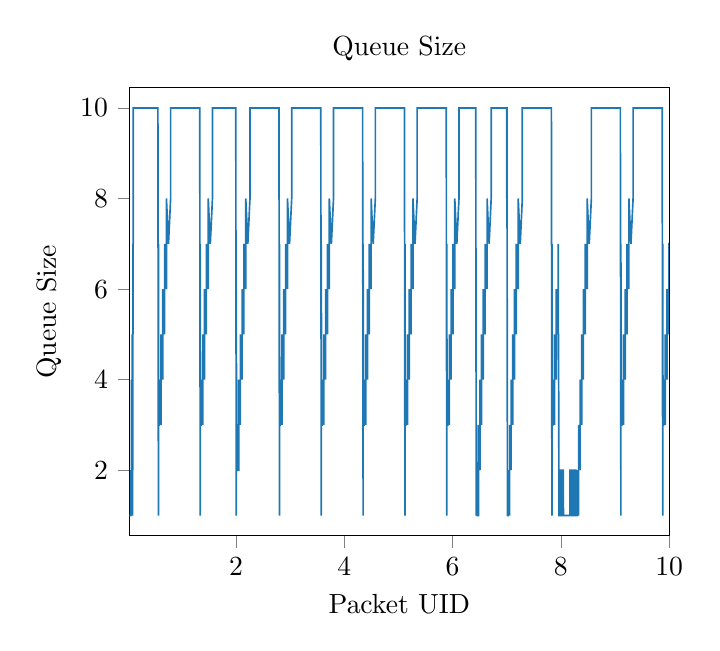
\begin{tikzpicture}

\definecolor{color0}{rgb}{0.12156862745098,0.466666666666667,0.705882352941177}

\begin{axis}[
title={Queue Size},
xlabel={Packet UID},
ylabel={Queue Size},
xmin=0.0332768, xmax=9.99745,
ymin=0.55, ymax=10.45,
tick align=outside,
tick pos=left,
x grid style={lightgray!92.026143790849673!black},
y grid style={lightgray!92.026143790849673!black}
]
\addplot [semithick, color0, forget plot]
table {%
0.0332768 1
0.0452512 1
0.0452512 1
0.0562816 1
0.0562816 1
0.0562816 2
0.0581696 1
0.0581696 2
0.068256 1
0.068256 2
0.070144 1
0.070144 3
0.072032 2
0.072032 3
0.072032 4
0.0802304 1
0.0802304 1
0.0802304 2
0.0821184 1
0.0821184 3
0.0840064 2
0.0840064 4
0.0858944 3
0.0858944 4
0.0858944 5
0.0912608 1
0.0912608 2
0.0912608 3
0.0931488 2
0.0931488 4
0.0950368 3
0.0950368 5
0.0969248 4
0.0969248 6
0.0988128 5
0.0988128 7
0.100701 6
0.100701 8
0.102589 7
0.104477 8
0.104477 10
0.556652 10
0.557596 10
0.55854 10
0.568278 1
0.568278 1
0.568278 2
0.568278 3
0.568278 4
0.568278 5
0.568278 6
0.568278 7
0.573644 3
0.574588 3
0.584972 3
0.585916 4
0.616124 3
0.616124 5
0.64822 4
0.64822 6
0.682204 5
0.682204 7
0.716188 6
0.716188 8
0.753948 7
0.793596 8
0.793596 10
1.32884 10
1.32979 10
1.33073 10
1.34047 1
1.34047 1
1.34047 2
1.34047 3
1.34047 4
1.34047 5
1.34047 6
1.34047 7
1.34584 3
1.34678 3
1.35716 3
1.35811 4
1.38832 3
1.38832 5
1.42041 4
1.42041 6
1.4544 5
1.4544 7
1.48838 6
1.48838 8
1.52614 7
1.56579 8
1.56579 10
1.99531 10
1.99625 10
2.00599 1
2.00599 1
2.00599 2
2.00599 3
2.00599 4
2.00599 6
2.01041 3
2.01135 3
2.02174 3
2.02457 2
2.051 2
2.051 4
2.08121 3
2.08121 5
2.11331 4
2.11331 6
2.1454 5
2.1454 7
2.18127 6
2.18127 8
2.21903 7
2.25868 8
2.25868 10
2.79204 10
2.79299 10
2.79393 10
2.80367 1
2.80367 1
2.80367 2
2.80367 3
2.80367 4
2.80367 5
2.80367 6
2.80367 7
2.80903 3
2.80998 3
2.82036 3
2.82131 4
2.85151 3
2.85151 5
2.88361 4
2.88361 6
2.91759 5
2.91759 7
2.95158 6
2.95158 8
2.98934 7
3.02899 8
3.02899 10
3.56423 10
3.56518 10
3.56612 10
3.57586 1
3.57586 1
3.57586 2
3.57586 3
3.57586 4
3.57586 5
3.57586 6
3.57586 7
3.58123 3
3.58217 3
3.59255 3
3.5935 4
3.62371 3
3.62371 5
3.6558 4
3.6558 6
3.68978 5
3.68978 7
3.72377 6
3.72377 8
3.76153 7
3.80118 8
3.80118 10
4.33642 10
4.33737 10
4.33831 10
4.34805 1
4.34805 1
4.34805 2
4.34805 3
4.34805 4
4.34805 5
4.34805 6
4.34805 7
4.35342 3
4.35436 3
4.36474 3
4.36569 4
4.3959 3
4.3959 5
4.42799 4
4.42799 6
4.46198 5
4.46198 7
4.49596 6
4.49596 8
4.53372 7
4.57337 8
4.57337 10
5.10862 10
5.10956 10
5.1105 10
5.12024 1
5.12024 1
5.12024 2
5.12024 3
5.12024 4
5.12024 5
5.12024 6
5.12024 7
5.12561 3
5.12655 3
5.13694 3
5.13788 4
5.16809 3
5.16809 5
5.20018 4
5.20018 6
5.23417 5
5.23417 7
5.26815 6
5.26815 8
5.30591 7
5.34556 8
5.34556 10
5.88081 10
5.88175 10
5.88269 10
5.89243 1
5.89243 1
5.89243 2
5.89243 3
5.89243 4
5.89243 5
5.89243 6
5.89243 7
5.8978 3
5.89874 3
5.90913 3
5.91007 4
5.94028 3
5.94028 5
5.97237 4
5.97237 6
6.00636 5
6.00636 7
6.04034 6
6.04034 8
6.0781 7
6.11775 8
6.11775 10
6.42644 10
6.42738 10
6.43712 1
6.43712 1
6.43712 2
6.43712 3
6.4406 2
6.44154 2
6.45098 2
6.45381 1
6.47836 1
6.47836 3
6.50668 2
6.50668 4
6.535 3
6.535 5
6.56709 4
6.56709 6
6.60108 5
6.60108 7
6.63695 6
6.63695 8
6.67471 7
6.71247 8
6.71247 10
6.99756 10
7.00039 8
7.00039 10
7.00133 10
7.00228 10
7.00322 10
7.01296 1
7.01296 1
7.01644 1
7.01738 1
7.02588 1
7.02682 2
7.05325 1
7.05325 3
7.08157 2
7.08157 4
7.10989 3
7.10989 5
7.14199 4
7.14199 6
7.17597 5
7.17597 7
7.21185 6
7.21185 8
7.24961 7
7.28737 8
7.28737 10
7.82261 10
7.82356 10
7.8245 10
7.83424 1
7.83424 1
7.83424 2
7.83424 3
7.83424 4
7.83424 5
7.83424 6
7.83424 7
7.8396 3
7.84055 3
7.85093 3
7.85188 4
7.88208 3
7.88208 5
7.91418 4
7.91418 6
7.94816 5
7.94816 7
7.95005 6
7.95005 7
7.95288 5
7.95383 5
7.95477 5
7.95572 5
7.96516 1
7.9661 1
7.98911 1
7.98911 2
7.99477 2
8.00108 1
8.014 1
8.014 2
8.01777 2
8.02314 1
8.04078 1
8.04078 2
8.04267 2
8.04709 1
8.11074 1
8.11988 1
8.13563 1
8.14383 1
8.16778 1
8.16778 2
8.16967 2
8.17692 1
8.19267 1
8.19267 2
8.19456 2
8.20087 1
8.22293 1
8.22293 2
8.22859 2
8.23396 1
8.24782 1
8.24782 2
8.25349 2
8.25791 1
8.2746 1
8.2746 2
8.27649 2
8.27997 1
8.30138 1
8.30138 2
8.32657 1
8.32657 3
8.35489 2
8.35489 4
8.3851 3
8.3851 5
8.41531 4
8.41531 6
8.44929 5
8.44929 7
8.48517 6
8.48517 8
8.52293 7
8.56257 8
8.56257 10
9.09593 10
9.09688 10
9.09782 10
9.10756 1
9.10756 1
9.10756 2
9.10756 3
9.10756 4
9.10756 5
9.10756 6
9.10756 7
9.11293 3
9.11387 3
9.12425 3
9.1252 4
9.15541 3
9.15541 5
9.1875 4
9.1875 6
9.22149 5
9.22149 7
9.25547 6
9.25547 8
9.29323 7
9.33288 8
9.33288 10
9.86812 10
9.86907 10
9.87001 10
9.87975 1
9.87975 1
9.87975 2
9.87975 3
9.87975 4
9.87975 5
9.87975 6
9.87975 7
9.88512 3
9.88606 3
9.89644 3
9.89739 4
9.9276 3
9.9276 5
9.95969 4
9.95969 6
9.99368 5
9.99368 7
9.99556 7
9.99745 6
9.99745 7
};
\end{axis}

\end{tikzpicture}% This file was created by matplotlib2tikz v0.6.13.
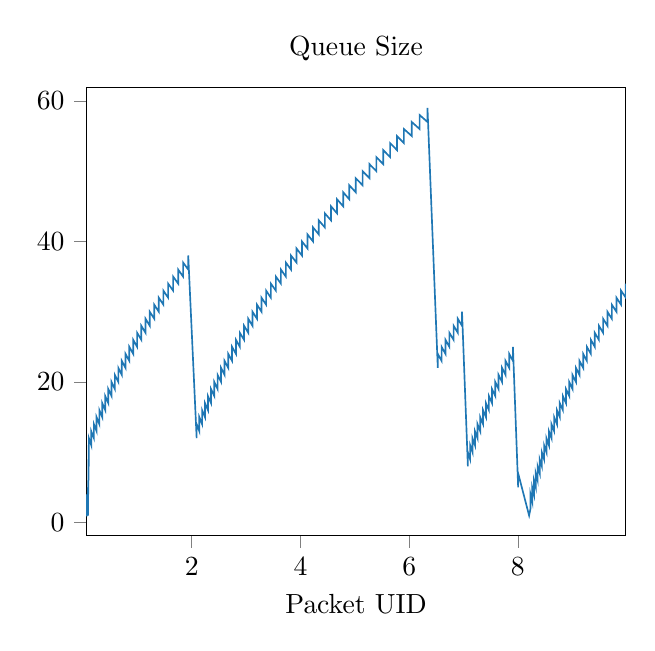
\begin{tikzpicture}

\definecolor{color0}{rgb}{0.12156862745098,0.466666666666667,0.705882352941177}

\begin{axis}[
title={Queue Size},
xlabel={Packet UID},
xmin=0.0581696, xmax=9.98458,
ymin=-1.9, ymax=61.9,
tick align=outside,
tick pos=left,
x grid style={lightgray!92.026143790849673!black},
y grid style={lightgray!92.026143790849673!black}
]
\addplot [semithick, color0, forget plot]
table {%
0.0581696 1
0.070144 1
0.072032 2
0.072032 4
0.0821184 1
0.0840064 2
0.0840064 4
0.0858944 3
0.0858944 5
0.0912608 1
0.0931488 2
0.0931488 4
0.0950368 3
0.0950368 5
0.0969248 4
0.0969248 6
0.0988128 5
0.0988128 7
0.100701 6
0.100701 8
0.102589 7
0.102589 9
0.104477 8
0.104477 10
0.106365 9
0.106365 11
0.108253 10
0.108253 12
0.151677 11
0.151677 13
0.200765 12
0.200765 14
0.249853 13
0.249853 15
0.300829 14
0.300829 16
0.353693 15
0.353693 17
0.408444 16
0.408444 18
0.465084 17
0.465084 19
0.5255 18
0.5255 20
0.585916 19
0.585916 21
0.650108 20
0.650108 22
0.7143 21
0.7143 23
0.782268 22
0.782268 24
0.852124 23
0.852124 25
0.923868 24
0.923868 26
0.995612 25
0.995612 27
1.07302 26
1.07302 28
1.15043 27
1.15043 29
1.22784 28
1.22784 30
1.31091 29
1.31091 31
1.39398 30
1.39398 32
1.47894 31
1.47894 33
1.56579 32
1.56579 34
1.6583 33
1.6583 35
1.75081 34
1.75081 36
1.84143 35
1.84143 37
1.93583 36
1.93583 38
2.09065 12
2.09065 14
2.13974 13
2.13974 15
2.19071 14
2.19071 16
2.24358 15
2.24358 17
2.29833 16
2.29833 18
2.35497 17
2.35497 19
2.41539 18
2.41539 20
2.4758 19
2.4758 21
2.53999 20
2.53999 22
2.60419 21
2.60419 23
2.67215 22
2.67215 24
2.74201 23
2.74201 25
2.81375 24
2.81375 26
2.8855 25
2.8855 27
2.96291 26
2.96291 28
3.04031 27
3.04031 29
3.11772 28
3.11772 30
3.20079 29
3.20079 31
3.28387 30
3.28387 32
3.36883 31
3.36883 33
3.45567 32
3.45567 34
3.54819 33
3.54819 35
3.6407 34
3.6407 36
3.73132 35
3.73132 37
3.82572 36
3.82572 38
3.92767 37
3.92767 39
4.02774 38
4.02774 40
4.12969 39
4.12969 41
4.23164 40
4.23164 42
4.33737 41
4.33737 43
4.44876 42
4.44876 44
4.56204 43
4.56204 45
4.67343 44
4.67343 46
4.78671 45
4.78671 47
4.8981 46
4.8981 48
5.01705 47
5.01705 49
5.14354 48
5.14354 50
5.27004 49
5.27004 51
5.39654 50
5.39654 52
5.52303 51
5.52303 53
5.64953 52
5.64953 54
5.77602 53
5.77602 55
5.90252 54
5.90252 56
6.04789 55
6.04789 57
6.19138 56
6.19138 58
6.33676 57
6.33676 59
6.5265 22
6.5265 24
6.59636 23
6.59636 25
6.6681 24
6.6681 26
6.73985 25
6.73985 27
6.81725 26
6.81725 28
6.89466 27
6.89466 29
6.97207 28
6.97207 30
7.07969 8
7.07969 10
7.12122 9
7.12122 11
7.16465 10
7.16465 12
7.20996 11
7.20996 13
7.25716 12
7.25716 14
7.30625 13
7.30625 15
7.35911 14
7.35911 16
7.41197 15
7.41197 17
7.46672 16
7.46672 18
7.52336 17
7.52336 19
7.58378 18
7.58378 20
7.6442 19
7.6442 21
7.70839 20
7.70839 22
7.77258 21
7.77258 23
7.84055 22
7.84055 24
7.90852 23
7.90852 25
8.0048 5
8.0048 7
8.20608 1
8.23251 2
8.23251 4
8.26272 3
8.26272 5
8.29482 4
8.29482 6
8.3288 5
8.3288 7
8.36278 6
8.36278 8
8.40054 7
8.40054 9
8.44019 8
8.44019 10
8.48173 9
8.48173 11
8.52515 10
8.52515 12
8.57046 11
8.57046 13
8.61766 12
8.61766 14
8.66675 13
8.66675 15
8.71773 14
8.71773 16
8.77059 15
8.77059 17
8.82723 16
8.82723 18
8.88387 17
8.88387 19
8.94429 18
8.94429 20
9.0047 19
9.0047 21
9.0689 20
9.0689 22
9.13309 21
9.13309 23
9.20106 22
9.20106 24
9.26902 23
9.26902 25
9.34266 24
9.34266 26
9.4144 25
9.4144 27
9.48992 26
9.48992 28
9.56733 27
9.56733 29
9.64662 28
9.64662 30
9.72781 29
9.72781 31
9.81277 30
9.81277 32
9.89773 31
9.89773 33
9.98458 32
9.98458 34
};
\end{axis}

\end{tikzpicture}\\
% This file was created by matplotlib2tikz v0.6.13.
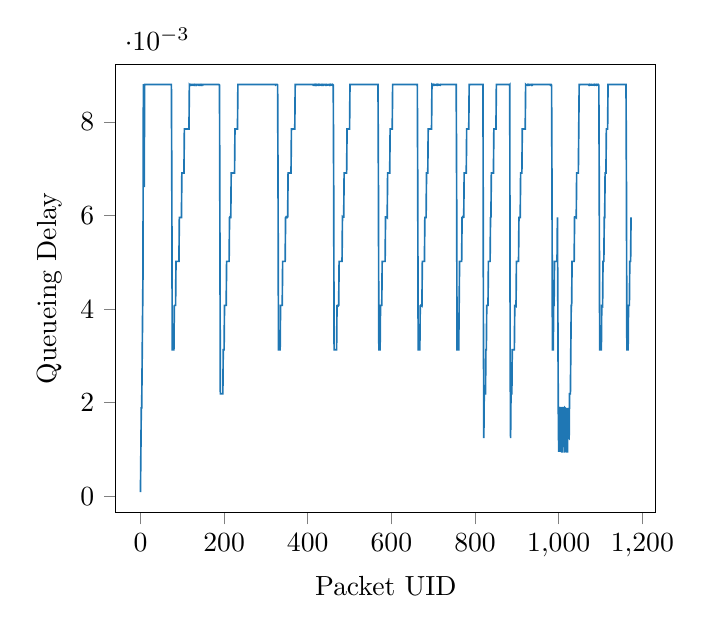
\begin{tikzpicture}

\definecolor{color0}{rgb}{0.12156862745098,0.466666666666667,0.705882352941177}

\begin{axis}[
xlabel={Packet UID},
ylabel={Queueing Delay},
xmin=-58.65, xmax=1231.65,
ymin=-0.000349280000000042, ymax=0.00923568000000085,
tick align=outside,
tick pos=left,
x grid style={lightgray!92.026143790849673!black},
y grid style={lightgray!92.026143790849673!black}
]
\addplot [semithick, color0, forget plot]
table {%
0 8.63999999999986e-05
1 0.000944000000000004
2 0.001888
3 0.00188800000000001
4 0.00283199999999999
5 0.003776
6 0.00471999999999999
7 0.00879400000000008
8 0.00879400000000008
9 0.00660800000000006
10 0.00879999999999992
11 0.00879999999999992
12 0.00880000000000014
13 0.00880000000000014
14 0.00879999999999992
15 0.00879999999999992
16 0.00879999999999992
17 0.00879999999999992
18 0.00879999999999992
19 0.00880000000000014
20 0.00880000000000014
21 0.00879999999999992
22 0.00879999999999992
23 0.00879999999999992
24 0.00879999999999992
25 0.00880000000000014
26 0.00880000000000014
27 0.00880000000000014
28 0.00879999999999992
29 0.00879999999999992
30 0.00879999999999992
31 0.00880000000000014
32 0.00880000000000014
33 0.00880000000000014
34 0.00879999999999992
35 0.00879999999999992
36 0.00879999999999992
37 0.00879999999999992
38 0.00880000000000014
39 0.00880000000000014
40 0.00880000000000014
41 0.00879999999999992
42 0.00879999999999992
43 0.00879999999999992
44 0.00879999999999992
45 0.00879999999999992
46 0.00880000000000014
47 0.00880000000000014
48 0.00879999999999992
49 0.00879999999999992
50 0.00879999999999992
51 0.00879999999999992
52 0.00880000000000014
53 0.00880000000000014
54 0.00880000000000014
55 0.00879999999999992
56 0.00879999999999992
57 0.00879999999999992
58 0.00880000000000014
59 0.00880000000000014
60 0.00879999999999992
61 0.00879999999999992
62 0.00879999999999992
63 0.00879999999999992
64 0.00880000000000014
65 0.00880000000000014
66 0.00880000000000014
67 0.00879999999999992
68 0.00879999999999992
69 0.00879999999999992
70 0.00880000000000014
71 0.00880000000000014
72 0.00880000000000014
73 0.00879999999999992
74 0.00879999999999992
75 0.00660999999999978
76 0.00313000000000008
77 0.00312999999999986
78 0.00313000000000008
79 0.0031300000000003
80 0.0031300000000003
81 0.0040699999999998
82 0.00408000000000008
83 0.00408000000000008
84 0.00408000000000008
85 0.00502000000000025
86 0.00502000000000002
87 0.00502000000000002
88 0.00502000000000002
89 0.00502000000000002
90 0.00502000000000002
91 0.00502000000000025
92 0.00502000000000002
93 0.00595999999999997
94 0.00595999999999997
95 0.00595999999999997
96 0.00595999999999997
97 0.00596000000000019
98 0.00596000000000019
99 0.00690999999999997
100 0.00690999999999997
101 0.00690999999999997
102 0.00691000000000019
103 0.00691000000000019
104 0.00690999999999997
105 0.00784999999999991
106 0.00784999999999991
107 0.00784999999999991
108 0.00784999999999991
109 0.00784999999999991
110 0.00785000000000013
111 0.00785000000000013
112 0.00785000000000013
113 0.00785000000000013
114 0.00785000000000013
115 0.00784999999999991
116 0.00784999999999991
117 0.00879999999999992
118 0.00879000000000008
119 0.00880000000000014
120 0.00879000000000008
121 0.00879999999999992
122 0.00879999999999992
123 0.00878999999999985
124 0.00879999999999992
125 0.00880000000000014
126 0.0087900000000003
127 0.00879999999999992
128 0.00880000000000014
129 0.00879000000000008
130 0.00880000000000014
131 0.0087900000000003
132 0.00880000000000014
133 0.00879999999999992
134 0.00879000000000008
135 0.00879999999999992
136 0.00880000000000014
137 0.00879999999999992
138 0.00879000000000008
139 0.00879999999999992
140 0.00880000000000014
141 0.0087900000000003
142 0.00880000000000014
143 0.00879999999999992
144 0.00879000000000008
145 0.00879999999999992
146 0.00879000000000008
147 0.00880000000000014
148 0.00879999999999992
149 0.00879000000000008
150 0.00879999999999992
151 0.00880000000000014
152 0.00880000000000014
153 0.00879999999999992
154 0.00879999999999992
155 0.00879999999999992
156 0.00879999999999992
157 0.00880000000000014
158 0.00880000000000014
159 0.00880000000000014
160 0.00880000000000014
161 0.00879999999999992
162 0.00879999999999992
163 0.00879999999999992
164 0.00880000000000014
165 0.00879999999999992
166 0.00879999999999992
167 0.00879999999999992
168 0.00879999999999992
169 0.00880000000000014
170 0.00880000000000014
171 0.00879999999999992
172 0.00879999999999992
173 0.00880000000000014
174 0.00879999999999992
175 0.00880000000000014
176 0.00880000000000014
177 0.00880000000000014
178 0.00879999999999992
179 0.00879999999999992
180 0.00879999999999992
181 0.00880000000000014
182 0.00880000000000014
183 0.00879999999999992
184 0.00879999999999992
185 0.00879999999999992
186 0.00880000000000014
187 0.00880000000000014
188 0.00879999999999992
189 0.00879000000000008
190 0.00565999999999978
191 0.00219000000000014
192 0.00219000000000014
193 0.00219000000000014
194 0.00219000000000014
195 0.00219000000000014
196 0.00219000000000014
197 0.00219000000000014
198 0.00313000000000008
199 0.00313000000000008
200 0.00313000000000052
201 0.00408000000000053
202 0.00408000000000008
203 0.00408000000000008
204 0.00408000000000008
205 0.00408000000000008
206 0.00502000000000002
207 0.00502000000000002
208 0.00502000000000002
209 0.00502000000000002
210 0.00502000000000002
211 0.00502000000000002
212 0.00502000000000047
213 0.00596000000000041
214 0.00597000000000003
215 0.00595999999999997
216 0.00596000000000041
217 0.00690999999999997
218 0.00690999999999997
219 0.00690999999999997
220 0.00691000000000042
221 0.00690999999999997
222 0.00690999999999997
223 0.00690999999999997
224 0.00691000000000042
225 0.00691000000000042
226 0.00784999999999991
227 0.00784999999999991
228 0.00784999999999991
229 0.00784999999999991
230 0.00784999999999991
231 0.00784999999999991
232 0.00784999999999991
233 0.00879999999999992
234 0.00880000000000036
235 0.00880000000000036
236 0.00879999999999992
237 0.00879999999999992
238 0.00879999999999992
239 0.00879999999999992
240 0.00879999999999992
241 0.00880000000000036
242 0.00879999999999992
243 0.00879999999999992
244 0.00879999999999992
245 0.00879999999999992
246 0.00880000000000036
247 0.00879999999999992
248 0.00879999999999992
249 0.00879999999999992
250 0.00879999999999992
251 0.00879999999999992
252 0.00879999999999992
253 0.00879999999999992
254 0.00879999999999992
255 0.00879999999999992
256 0.00879999999999992
257 0.00879999999999992
258 0.00879999999999992
259 0.00879999999999992
260 0.00879999999999992
261 0.00879999999999992
262 0.00879999999999992
263 0.00879999999999992
264 0.00879999999999992
265 0.00879999999999992
266 0.00880000000000036
267 0.00879999999999992
268 0.00879999999999992
269 0.00879999999999992
270 0.00879999999999992
271 0.00879999999999992
272 0.00879999999999992
273 0.00879999999999992
274 0.00879999999999992
275 0.00880000000000036
276 0.00879999999999992
277 0.00879999999999992
278 0.00879999999999992
279 0.00879999999999992
280 0.00880000000000036
281 0.00880000000000036
282 0.00879999999999992
283 0.00879999999999992
284 0.00880000000000036
285 0.00879999999999992
286 0.00880000000000036
287 0.00879999999999992
288 0.00879999999999992
289 0.00880000000000036
290 0.00880000000000036
291 0.00879999999999992
292 0.00879999999999992
293 0.00879999999999992
294 0.00879999999999992
295 0.00880000000000036
296 0.00879999999999992
297 0.00879999999999992
298 0.00879999999999992
299 0.00879999999999992
300 0.00880000000000036
301 0.00879999999999992
302 0.00880000000000036
303 0.00879999999999992
304 0.00879999999999992
305 0.00879999999999992
306 0.00879999999999992
307 0.00879999999999992
308 0.00880000000000036
309 0.00879999999999992
310 0.00879999999999992
311 0.00879999999999992
312 0.00879999999999992
313 0.00879999999999992
314 0.00879999999999992
315 0.00880000000000036
316 0.00879999999999992
317 0.00879999999999992
318 0.00879999999999992
319 0.00879999999999992
320 0.00879999999999992
321 0.00879999999999992
322 0.00879999999999992
323 0.0087900000000003
324 0.00879999999999992
325 0.00879999999999992
326 0.00879999999999992
327 0.00879999999999992
328 0.00878999999999985
329 0.00661000000000023
330 0.00313000000000052
331 0.00313000000000008
332 0.00313000000000008
333 0.00313000000000008
334 0.00313000000000008
335 0.00408000000000053
336 0.00408000000000008
337 0.00408000000000008
338 0.00408000000000008
339 0.00408000000000008
340 0.00502000000000002
341 0.00502000000000002
342 0.00502000000000002
343 0.00502000000000002
344 0.00502000000000002
345 0.00502000000000047
346 0.00502000000000047
347 0.00595999999999997
348 0.00597000000000047
349 0.00595999999999997
350 0.00597000000000003
351 0.00595999999999997
352 0.00597000000000003
353 0.00690999999999997
354 0.00690999999999997
355 0.00691000000000042
356 0.00691000000000042
357 0.00691000000000042
358 0.00690999999999997
359 0.00690999999999997
360 0.00690999999999997
361 0.00784999999999991
362 0.00784999999999991
363 0.00784999999999991
364 0.00785000000000036
365 0.00784999999999991
366 0.00784999999999991
367 0.00784999999999991
368 0.00784999999999991
369 0.00784999999999991
370 0.00880000000000036
371 0.00880000000000036
372 0.00879999999999992
373 0.00879999999999992
374 0.00879999999999992
375 0.00879999999999992
376 0.00880000000000036
377 0.00880000000000036
378 0.00879999999999992
379 0.00879999999999992
380 0.00879999999999992
381 0.00879999999999992
382 0.00879999999999992
383 0.00880000000000036
384 0.00879999999999992
385 0.00879999999999992
386 0.00879999999999992
387 0.00879999999999992
388 0.00880000000000036
389 0.00880000000000036
390 0.00879999999999992
391 0.00879999999999992
392 0.00879999999999992
393 0.00879999999999992
394 0.00879999999999992
395 0.00879999999999992
396 0.00879999999999992
397 0.00879999999999992
398 0.00879999999999992
399 0.00879999999999992
400 0.00879999999999992
401 0.00879999999999992
402 0.00879999999999992
403 0.00879999999999992
404 0.00879999999999992
405 0.00879999999999992
406 0.00879999999999992
407 0.00880000000000036
408 0.00879999999999992
409 0.00879999999999992
410 0.00879999999999992
411 0.00879999999999992
412 0.00879999999999992
413 0.00878999999999985
414 0.00879999999999992
415 0.00879999999999992
416 0.0087900000000003
417 0.00879999999999992
418 0.0087900000000003
419 0.00879999999999992
420 0.0087900000000003
421 0.00879999999999992
422 0.00878999999999985
423 0.00879999999999992
424 0.00880000000000036
425 0.0087900000000003
426 0.00880000000000036
427 0.0087900000000003
428 0.00880000000000036
429 0.0087900000000003
430 0.0087900000000003
431 0.00879999999999992
432 0.00879999999999992
433 0.0087900000000003
434 0.00879999999999992
435 0.0087900000000003
436 0.00879999999999992
437 0.00879999999999992
438 0.0087900000000003
439 0.00879999999999992
440 0.00879999999999992
441 0.00879999999999992
442 0.00878999999999985
443 0.00880000000000036
444 0.00880000000000036
445 0.0087900000000003
446 0.00879999999999992
447 0.0087900000000003
448 0.0087900000000003
449 0.0087900000000003
450 0.00879999999999992
451 0.00879999999999992
452 0.0087900000000003
453 0.00879999999999992
454 0.0087900000000003
455 0.00879999999999992
456 0.0087900000000003
457 0.0087900000000003
458 0.00879999999999992
459 0.0087900000000003
460 0.00879999999999992
461 0.0087900000000003
462 0.00660999999999978
463 0.00313000000000008
464 0.00313000000000052
465 0.00312999999999963
466 0.00313000000000008
467 0.00312999999999963
468 0.00312999999999963
469 0.00313000000000052
470 0.00407000000000046
471 0.00407000000000002
472 0.00408000000000053
473 0.00407000000000002
474 0.00408000000000053
475 0.00501999999999958
476 0.00501999999999958
477 0.00502000000000002
478 0.00501999999999958
479 0.00502000000000002
480 0.00502000000000047
481 0.00502000000000047
482 0.00502000000000047
483 0.00597000000000047
484 0.00595999999999997
485 0.00597000000000003
486 0.00596999999999959
487 0.00691000000000042
488 0.00691000000000042
489 0.00690999999999997
490 0.00691000000000086
491 0.00690999999999997
492 0.00690999999999997
493 0.00690999999999997
494 0.00784999999999991
495 0.00784999999999991
496 0.00784999999999991
497 0.00784999999999991
498 0.00784999999999991
499 0.00784999999999991
500 0.00784999999999991
501 0.00880000000000036
502 0.00880000000000036
503 0.00879999999999992
504 0.00879999999999992
505 0.00879999999999992
506 0.00879999999999992
507 0.00879999999999992
508 0.00879999999999992
509 0.00879999999999992
510 0.00879999999999992
511 0.00879999999999992
512 0.00879999999999992
513 0.00879999999999992
514 0.00879999999999992
515 0.00879999999999992
516 0.00880000000000036
517 0.00879999999999992
518 0.00880000000000036
519 0.00880000000000036
520 0.00879999999999992
521 0.00880000000000036
522 0.00880000000000036
523 0.00880000000000036
524 0.00879999999999992
525 0.00879999999999992
526 0.00879999999999992
527 0.00879999999999992
528 0.00879999999999992
529 0.00879999999999992
530 0.00879999999999992
531 0.00879999999999992
532 0.00880000000000036
533 0.00880000000000081
534 0.00879999999999992
535 0.00879999999999992
536 0.00879999999999992
537 0.00880000000000081
538 0.00879999999999992
539 0.00880000000000081
540 0.00879999999999992
541 0.00879999999999992
542 0.00879999999999992
543 0.00879999999999992
544 0.00879999999999992
545 0.00879999999999992
546 0.00879999999999992
547 0.00880000000000081
548 0.00879999999999992
549 0.00879999999999992
550 0.00879999999999992
551 0.00880000000000081
552 0.00879999999999992
553 0.00879999999999992
554 0.00879999999999992
555 0.00879999999999992
556 0.00879999999999992
557 0.00879999999999992
558 0.00879999999999992
559 0.00879999999999992
560 0.00880000000000081
561 0.00879999999999992
562 0.00879999999999992
563 0.00879999999999992
564 0.00879999999999992
565 0.00879999999999992
566 0.00879999999999992
567 0.00879999999999992
568 0.00879999999999992
569 0.00661000000000023
570 0.00312999999999963
571 0.00312999999999963
572 0.00313000000000052
573 0.00313000000000052
574 0.00408000000000008
575 0.00408000000000008
576 0.00408000000000097
577 0.00408000000000008
578 0.00502000000000091
579 0.00502000000000091
580 0.00502000000000002
581 0.00502000000000091
582 0.00502000000000002
583 0.00502000000000002
584 0.00502000000000002
585 0.00502000000000002
586 0.00597000000000047
587 0.00596999999999959
588 0.00596000000000085
589 0.00597000000000047
590 0.00595999999999997
591 0.00691000000000042
592 0.00691000000000042
593 0.00691000000000042
594 0.00691000000000042
595 0.00690999999999953
596 0.00691000000000042
597 0.00785000000000036
598 0.00785000000000036
599 0.00785000000000036
600 0.00785000000000036
601 0.00785000000000036
602 0.00785000000000036
603 0.00879999999999992
604 0.00879999999999992
605 0.00880000000000081
606 0.00879999999999992
607 0.00879999999999992
608 0.00880000000000081
609 0.00879999999999992
610 0.00879999999999992
611 0.00880000000000081
612 0.00879999999999992
613 0.00879999999999992
614 0.00879999999999992
615 0.00879999999999992
616 0.00879999999999992
617 0.00880000000000081
618 0.00879999999999992
619 0.00879999999999992
620 0.00879999999999992
621 0.00880000000000081
622 0.00879999999999992
623 0.00879999999999992
624 0.00879999999999992
625 0.00879999999999992
626 0.00879999999999992
627 0.00879999999999992
628 0.00879999999999992
629 0.00879999999999992
630 0.00879999999999992
631 0.00880000000000081
632 0.00879999999999992
633 0.00879999999999992
634 0.00880000000000081
635 0.00879999999999992
636 0.00880000000000081
637 0.00879999999999992
638 0.00879999999999992
639 0.00879999999999992
640 0.00879999999999992
641 0.00879999999999992
642 0.00879999999999992
643 0.00879999999999992
644 0.00879999999999992
645 0.00880000000000081
646 0.00879999999999992
647 0.00879999999999992
648 0.00880000000000081
649 0.00879999999999992
650 0.00879999999999992
651 0.00879999999999992
652 0.00879999999999992
653 0.00879999999999992
654 0.00879999999999992
655 0.00879999999999992
656 0.00879999999999992
657 0.00880000000000081
658 0.00879999999999992
659 0.00879999999999992
660 0.00880000000000081
661 0.00879999999999992
662 0.00879999999999992
663 0.00661000000000023
664 0.00313000000000052
665 0.00313000000000052
666 0.00313000000000052
667 0.00313000000000052
668 0.00313000000000052
669 0.00406999999999957
670 0.00408000000000008
671 0.00407000000000046
672 0.00408000000000008
673 0.00407000000000046
674 0.00502000000000091
675 0.00502000000000091
676 0.00502000000000002
677 0.00502000000000091
678 0.00502000000000002
679 0.00502000000000002
680 0.00596000000000085
681 0.00595999999999997
682 0.00595999999999997
683 0.00595999999999997
684 0.00691000000000042
685 0.00691000000000042
686 0.0069100000000013
687 0.00691000000000042
688 0.00785000000000036
689 0.00785000000000036
690 0.00785000000000036
691 0.00785000000000036
692 0.00785000000000036
693 0.00785000000000036
694 0.00785000000000036
695 0.00785000000000036
696 0.00785000000000036
697 0.00879999999999992
698 0.0087900000000003
699 0.00879999999999992
700 0.0087900000000003
701 0.00879999999999992
702 0.0087900000000003
703 0.00880000000000081
704 0.00879999999999992
705 0.0087900000000003
706 0.0087900000000003
707 0.0087900000000003
708 0.00879999999999992
709 0.0087900000000003
710 0.00879999999999992
711 0.0087900000000003
712 0.00879999999999992
713 0.0087900000000003
714 0.0087900000000003
715 0.0087900000000003
716 0.00879999999999992
717 0.0087900000000003
718 0.00880000000000081
719 0.00879999999999992
720 0.00879999999999992
721 0.00879999999999992
722 0.00879999999999992
723 0.00879999999999992
724 0.00880000000000081
725 0.00879999999999992
726 0.00879999999999992
727 0.00879999999999992
728 0.00880000000000081
729 0.00879999999999992
730 0.00879999999999992
731 0.00879999999999992
732 0.00879999999999992
733 0.00879999999999992
734 0.00879999999999992
735 0.00879999999999992
736 0.00880000000000081
737 0.00879999999999992
738 0.00879999999999992
739 0.00880000000000081
740 0.00879999999999992
741 0.00880000000000081
742 0.00879999999999992
743 0.00879999999999992
744 0.00879999999999992
745 0.00879999999999992
746 0.00879999999999992
747 0.00879999999999992
748 0.00880000000000081
749 0.00879999999999992
750 0.00879999999999992
751 0.00880000000000081
752 0.00879999999999992
753 0.00879999999999992
754 0.00880000000000081
755 0.00879999999999992
756 0.00661000000000023
757 0.00313000000000052
758 0.00313000000000052
759 0.00313000000000052
760 0.00312999999999963
761 0.00312999999999963
762 0.00408000000000008
763 0.00502000000000002
764 0.00502000000000002
765 0.00502000000000002
766 0.00502000000000002
767 0.00502000000000091
768 0.00502000000000091
769 0.00595999999999997
770 0.00597000000000047
771 0.00595999999999997
772 0.00597000000000047
773 0.00596999999999959
774 0.00691000000000042
775 0.00691000000000042
776 0.00691000000000042
777 0.00691000000000042
778 0.00691000000000042
779 0.00691000000000042
780 0.00785000000000036
781 0.00785000000000036
782 0.00785000000000036
783 0.00785000000000036
784 0.00785000000000036
785 0.00785000000000036
786 0.00879999999999992
787 0.00879999999999992
788 0.00879999999999992
789 0.00879999999999992
790 0.00879999999999992
791 0.00879999999999992
792 0.00879999999999992
793 0.00880000000000081
794 0.00879999999999992
795 0.00879999999999992
796 0.00879999999999992
797 0.00880000000000081
798 0.00879999999999992
799 0.00880000000000081
800 0.00879999999999992
801 0.00879999999999992
802 0.00879999999999992
803 0.00879999999999992
804 0.00879999999999992
805 0.00879999999999992
806 0.00880000000000081
807 0.00879999999999992
808 0.00879999999999992
809 0.00880000000000081
810 0.00879999999999992
811 0.00879999999999992
812 0.00879999999999992
813 0.00879999999999992
814 0.00879999999999992
815 0.00879999999999992
816 0.00879999999999992
817 0.00879999999999992
818 0.00880000000000081
819 0.00879999999999992
820 0.00378000000000078
821 0.00124000000000013
822 0.00219000000000058
823 0.00219000000000058
824 0.00219000000000058
825 0.00219000000000058
826 0.00313000000000052
827 0.00313000000000052
828 0.00408000000000008
829 0.00408000000000097
830 0.00408000000000097
831 0.00408000000000008
832 0.00502000000000002
833 0.00502000000000002
834 0.00502000000000002
835 0.0050200000000018
836 0.0050200000000018
837 0.00596000000000085
838 0.00597000000000136
839 0.0069100000000013
840 0.00691000000000042
841 0.00691000000000042
842 0.00691000000000042
843 0.00691000000000042
844 0.00691000000000042
845 0.00785000000000036
846 0.00785000000000036
847 0.00785000000000036
848 0.00785000000000036
849 0.00785000000000036
850 0.00785000000000036
851 0.00879999999999992
852 0.00879999999999992
853 0.00879999999999992
854 0.00879999999999992
855 0.00879999999999992
856 0.00879999999999992
857 0.00880000000000081
858 0.00879999999999992
859 0.00879999999999992
860 0.00880000000000081
861 0.00879999999999992
862 0.00879999999999992
863 0.00879999999999992
864 0.00879999999999992
865 0.00879999999999992
866 0.00879999999999992
867 0.00879999999999992
868 0.00879999999999992
869 0.00879999999999992
870 0.00880000000000081
871 0.00879999999999992
872 0.00879999999999992
873 0.00880000000000081
874 0.00879999999999992
875 0.00879999999999992
876 0.00879999999999992
877 0.00879999999999992
878 0.00879999999999992
879 0.00879999999999992
880 0.00880000000000081
881 0.00879999999999992
882 0.00878999999999941
883 0.00879999999999992
884 0.00282999999999856
885 0.00124000000000102
886 0.00219000000000058
887 0.00219000000000147
888 0.00219000000000058
889 0.00313000000000052
890 0.00313000000000052
891 0.00313000000000052
892 0.00313000000000052
893 0.00313000000000052
894 0.00313000000000052
895 0.00408000000000097
896 0.00408000000000008
897 0.00408000000000097
898 0.00407000000000135
899 0.00502000000000091
900 0.0050200000000018
901 0.00502000000000002
902 0.00502000000000091
903 0.00502000000000002
904 0.00502000000000002
905 0.00595999999999997
906 0.00596000000000085
907 0.00595999999999997
908 0.00596000000000085
909 0.00691000000000042
910 0.00691000000000042
911 0.0069100000000013
912 0.00691000000000042
913 0.00785000000000036
914 0.00785000000000036
915 0.00785000000000036
916 0.00785000000000036
917 0.00785000000000036
918 0.00785000000000036
919 0.00785000000000036
920 0.00785000000000036
921 0.00879999999999992
922 0.00879000000000119
923 0.00878999999999941
924 0.00879000000000119
925 0.00879999999999992
926 0.00879000000000119
927 0.00879999999999992
928 0.00879000000000119
929 0.00879999999999992
930 0.00879999999999992
931 0.00879000000000119
932 0.00880000000000081
933 0.00879999999999992
934 0.00880000000000081
935 0.0087900000000003
936 0.00879999999999992
937 0.00879000000000119
938 0.00879999999999992
939 0.00879999999999992
940 0.00879999999999992
941 0.00880000000000081
942 0.00879999999999992
943 0.00879999999999992
944 0.00879999999999992
945 0.00880000000000081
946 0.00879999999999992
947 0.00880000000000081
948 0.00879999999999992
949 0.00879999999999992
950 0.00879999999999992
951 0.00879999999999992
952 0.00879999999999992
953 0.00879999999999992
954 0.00879999999999992
955 0.00879999999999992
956 0.00880000000000081
957 0.00879999999999992
958 0.00879999999999992
959 0.00879999999999992
960 0.00879999999999992
961 0.00879999999999992
962 0.00879999999999992
963 0.00879999999999992
964 0.00880000000000081
965 0.00879999999999992
966 0.00879999999999992
967 0.00879999999999992
968 0.00880000000000081
969 0.00879999999999992
970 0.00879999999999992
971 0.00880000000000081
972 0.00879999999999992
973 0.00879999999999992
974 0.00879999999999992
975 0.00879999999999992
976 0.00879999999999992
977 0.00879999999999992
978 0.00879999999999992
979 0.00879999999999992
980 0.00878999999999941
981 0.00880000000000081
982 0.00879999999999992
983 0.00878999999999941
984 0.00661000000000023
985 0.00313000000000052
986 0.00313000000000141
987 0.00313000000000052
988 0.00408000000000008
989 0.00408000000000008
990 0.00502000000000002
991 0.00502000000000002
992 0.00502000000000002
993 0.00502000000000002
994 0.00502000000000002
995 0.00502000000000002
996 0.00502000000000091
997 0.00596000000000085
998 0.00406999999999957
999 0.00189000000000039
1000 0.000950000000001339
1001 0.0018899999999995
1002 0.00187999999999988
1003 0.000950000000001339
1004 0.00189000000000128
1005 0.0018899999999995
1006 0.00187999999999988
1007 0.000950000000001339
1008 0.000950000000001339
1009 0.00189000000000128
1010 0.0018899999999995
1011 0.00189000000000128
1012 0.00189000000000128
1013 0.000950000000001339
1014 0.000950000000001339
1015 0.00189000000000128
1016 0.00187999999999988
1017 0.000950000000001339
1018 0.00189000000000128
1019 0.000950000000001339
1020 0.000950000000001339
1021 0.000950000000001339
1022 0.0018899999999995
1023 0.00124000000000102
1024 0.00125000000000064
1025 0.00123999999999924
1026 0.00219000000000058
1027 0.00219000000000058
1028 0.00219000000000058
1029 0.00313000000000052
1030 0.00408000000000008
1031 0.00408000000000008
1032 0.0050200000000018
1033 0.0050200000000018
1034 0.00502000000000002
1035 0.0050200000000018
1036 0.00502000000000002
1037 0.00502000000000002
1038 0.00597000000000136
1039 0.00596999999999959
1040 0.00596000000000174
1041 0.00597000000000136
1042 0.00595999999999997
1043 0.0069100000000013
1044 0.0069100000000013
1045 0.00690999999999953
1046 0.0069100000000013
1047 0.0069100000000013
1048 0.00785000000000124
1049 0.00880000000000081
1050 0.00880000000000081
1051 0.00880000000000081
1052 0.00880000000000081
1053 0.00880000000000081
1054 0.00880000000000081
1055 0.00880000000000081
1056 0.00880000000000081
1057 0.00880000000000081
1058 0.00880000000000081
1059 0.00880000000000081
1060 0.00880000000000081
1061 0.00880000000000081
1062 0.00880000000000081
1063 0.00880000000000081
1064 0.00880000000000081
1065 0.00880000000000081
1066 0.00880000000000081
1067 0.00880000000000081
1068 0.00880000000000081
1069 0.00880000000000081
1070 0.00880000000000081
1071 0.00880000000000081
1072 0.00879000000000119
1073 0.00880000000000081
1074 0.00878999999999941
1075 0.00880000000000081
1076 0.00879000000000119
1077 0.00879000000000119
1078 0.00880000000000081
1079 0.00878999999999941
1080 0.00879000000000119
1081 0.00879000000000119
1082 0.00880000000000081
1083 0.00878999999999941
1084 0.00879000000000119
1085 0.00880000000000081
1086 0.00879000000000119
1087 0.00880000000000081
1088 0.00878999999999941
1089 0.00879000000000119
1090 0.00880000000000081
1091 0.00879000000000119
1092 0.00880000000000081
1093 0.00878999999999941
1094 0.00879000000000119
1095 0.00880000000000081
1096 0.00878999999999941
1097 0.00660999999999845
1098 0.00313000000000052
1099 0.00313000000000052
1100 0.00313000000000052
1101 0.00313000000000052
1102 0.00313000000000052
1103 0.00408000000000008
1104 0.00408000000000008
1105 0.00407000000000046
1106 0.0050200000000018
1107 0.00502000000000002
1108 0.00502000000000002
1109 0.00595999999999997
1110 0.00595999999999997
1111 0.0069100000000013
1112 0.0069100000000013
1113 0.0069100000000013
1114 0.00785000000000124
1115 0.00785000000000124
1116 0.00785000000000124
1117 0.00785000000000124
1118 0.00880000000000081
1119 0.00880000000000081
1120 0.00880000000000081
1121 0.00880000000000081
1122 0.00880000000000081
1123 0.00880000000000081
1124 0.00880000000000081
1125 0.00880000000000081
1126 0.00880000000000081
1127 0.00880000000000081
1128 0.00880000000000081
1129 0.00880000000000081
1130 0.00880000000000081
1131 0.00880000000000081
1132 0.00880000000000081
1133 0.00880000000000081
1134 0.00880000000000081
1135 0.00880000000000081
1136 0.00880000000000081
1137 0.00880000000000081
1138 0.00880000000000081
1139 0.00880000000000081
1140 0.00880000000000081
1141 0.00880000000000081
1142 0.00880000000000081
1143 0.00880000000000081
1144 0.00880000000000081
1145 0.00880000000000081
1146 0.00880000000000081
1147 0.00880000000000081
1148 0.00880000000000081
1149 0.00880000000000081
1150 0.00880000000000081
1151 0.00880000000000081
1152 0.00880000000000081
1153 0.00880000000000081
1154 0.00880000000000081
1155 0.00880000000000081
1156 0.00880000000000081
1157 0.00880000000000081
1158 0.00880000000000081
1159 0.00880000000000081
1160 0.00880000000000081
1161 0.00880000000000081
1162 0.00661000000000023
1163 0.00313000000000052
1164 0.00313000000000052
1165 0.00313000000000052
1166 0.00313000000000052
1167 0.00408000000000008
1168 0.00408000000000008
1169 0.00408000000000008
1170 0.00502000000000002
1171 0.00502000000000002
1172 0.00502000000000002
1173 0.00595999999999997
};
\end{axis}

\end{tikzpicture}% This file was created by matplotlib2tikz v0.6.13.
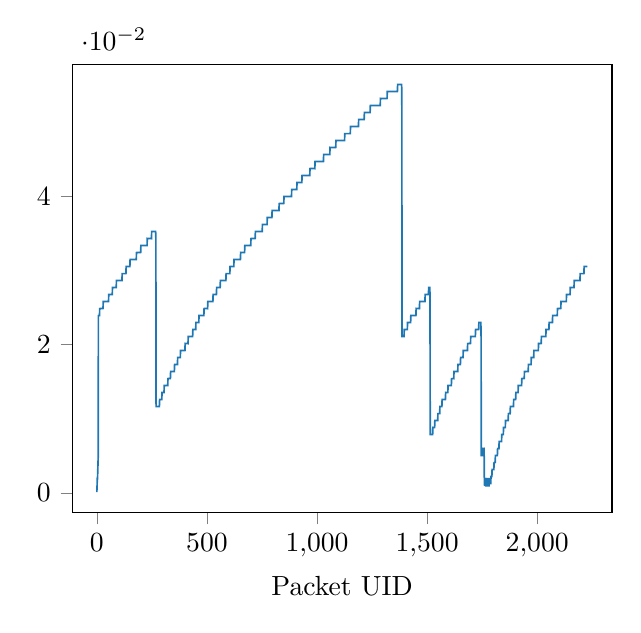
\begin{tikzpicture}

\definecolor{color0}{rgb}{0.12156862745098,0.466666666666667,0.705882352941177}

\begin{axis}[
xlabel={Packet UID},
xmin=-111.4, xmax=2339.4,
ymin=-0.00266178000000003, ymax=0.0577981800000005,
tick align=outside,
tick pos=left,
x grid style={lightgray!92.026143790849673!black},
y grid style={lightgray!92.026143790849673!black}
]
\addplot [semithick, color0, forget plot]
table {%
0 8.63999999999986e-05
1 0.000944000000000004
2 0.001888
3 0.00188800000000001
4 0.00283199999999999
5 0.003776
6 0.00471999999999999
7 0.023898
8 0.0239
9 0.023902
10 0.0238980000000001
11 0.0238999999999999
12 0.023902
13 0.024842
14 0.02485
15 0.0248400000000002
16 0.02485
17 0.02484
18 0.0248499999999998
19 0.02484
20 0.02485
21 0.02484
22 0.02485
23 0.02484
24 0.02485
25 0.02484
26 0.0248499999999998
27 0.02484
28 0.02485
29 0.02579
30 0.0257900000000002
31 0.02579
32 0.02579
33 0.02579
34 0.0257899999999998
35 0.02579
36 0.02579
37 0.02579
38 0.02579
39 0.02579
40 0.02579
41 0.0257900000000002
42 0.02579
43 0.0257900000000002
44 0.02579
45 0.02579
46 0.02579
47 0.02579
48 0.02579
49 0.02579
50 0.02579
51 0.02579
52 0.02579
53 0.02579
54 0.0267300000000001
55 0.0267299999999999
56 0.0267299999999999
57 0.0267299999999999
58 0.0267299999999999
59 0.0267299999999999
60 0.0267299999999999
61 0.0267299999999999
62 0.0267300000000001
63 0.0267300000000001
64 0.0267300000000001
65 0.0267300000000001
66 0.0267299999999999
67 0.0267299999999999
68 0.0267299999999999
69 0.0267300000000001
70 0.0267299999999999
71 0.0276799999999999
72 0.0276799999999999
73 0.0276799999999999
74 0.0276799999999999
75 0.0276799999999999
76 0.0276800000000001
77 0.0276799999999999
78 0.0276800000000001
79 0.0276800000000001
80 0.0276799999999999
81 0.0276799999999999
82 0.0276799999999999
83 0.0276799999999999
84 0.0276799999999999
85 0.0276799999999999
86 0.0276800000000001
87 0.0276800000000001
88 0.0276800000000001
89 0.0286199999999999
90 0.0286199999999999
91 0.0286199999999999
92 0.0286200000000001
93 0.0286199999999999
94 0.0286200000000001
95 0.0286200000000001
96 0.0286200000000001
97 0.0286200000000001
98 0.0286200000000001
99 0.0286200000000001
100 0.0286200000000001
101 0.0286199999999999
102 0.0286199999999999
103 0.0286200000000001
104 0.0286200000000001
105 0.0286199999999999
106 0.0286199999999999
107 0.0286199999999999
108 0.0286199999999999
109 0.0286200000000001
110 0.0286199999999999
111 0.0286200000000001
112 0.0286200000000001
113 0.0286199999999999
114 0.0286200000000001
115 0.02956
116 0.0295599999999998
117 0.0295599999999998
118 0.02956
119 0.02956
120 0.02956
121 0.02956
122 0.02956
123 0.02956
124 0.02956
125 0.02956
126 0.0295599999999998
127 0.0295599999999998
128 0.02956
129 0.02956
130 0.02956
131 0.02956
132 0.02956
133 0.03051
134 0.03051
135 0.03051
136 0.03051
137 0.03051
138 0.0305099999999998
139 0.0305099999999998
140 0.03051
141 0.03051
142 0.03051
143 0.03051
144 0.03051
145 0.03051
146 0.03051
147 0.03051
148 0.0305099999999998
149 0.0305099999999998
150 0.03051
151 0.03145
152 0.03145
153 0.03145
154 0.03145
155 0.03145
156 0.03145
157 0.03145
158 0.03145
159 0.0314500000000002
160 0.03145
161 0.03145
162 0.03145
163 0.03145
164 0.0314499999999998
165 0.03145
166 0.0314500000000002
167 0.03145
168 0.0314500000000002
169 0.0314500000000002
170 0.0314500000000002
171 0.03145
172 0.03145
173 0.03145
174 0.03145
175 0.03145
176 0.03145
177 0.03145
178 0.03145
179 0.03145
180 0.0323899999999999
181 0.0324
182 0.0323900000000001
183 0.0324
184 0.0323899999999997
185 0.0324
186 0.0323900000000001
187 0.0324
188 0.0323900000000001
189 0.0324
190 0.0323899999999997
191 0.0324
192 0.0323900000000001
193 0.0324000000000002
194 0.0323899999999999
195 0.0324
196 0.0323900000000001
197 0.0324
198 0.0323900000000001
199 0.0324
200 0.0333400000000001
201 0.0333400000000001
202 0.0333400000000001
203 0.0333400000000001
204 0.0333399999999999
205 0.0333400000000001
206 0.0333399999999997
207 0.0333400000000001
208 0.0333399999999997
209 0.0333400000000001
210 0.0333399999999997
211 0.0333400000000001
212 0.0333399999999999
213 0.0333400000000001
214 0.0333399999999997
215 0.0333400000000001
216 0.0333400000000001
217 0.0333400000000001
218 0.0333400000000001
219 0.0333399999999997
220 0.0333400000000001
221 0.0333399999999997
222 0.0333400000000001
223 0.0333399999999999
224 0.0333400000000001
225 0.0333399999999997
226 0.0333400000000001
227 0.0333399999999997
228 0.0333400000000001
229 0.0342900000000002
230 0.0342799999999999
231 0.0342899999999999
232 0.0342800000000001
233 0.0342900000000002
234 0.0342799999999999
235 0.0342900000000002
236 0.0342799999999999
237 0.0342899999999997
238 0.0342800000000003
239 0.0342899999999999
240 0.0342799999999999
241 0.0342899999999997
242 0.0342799999999999
243 0.0342900000000002
244 0.0342799999999999
245 0.0342900000000002
246 0.0342800000000001
247 0.0342899999999999
248 0.0342800000000003
249 0.0352299999999999
250 0.0352299999999999
251 0.0352300000000003
252 0.0352299999999999
253 0.0352300000000003
254 0.0352299999999999
255 0.0352300000000001
256 0.0352300000000001
257 0.0352300000000001
258 0.0352299999999999
259 0.0352299999999997
260 0.0352299999999999
261 0.0352299999999999
262 0.0352300000000001
263 0.0352299999999999
264 0.0352299999999999
265 0.0352300000000001
266 0.0352300000000001
267 0.0352299999999999
268 0.0342799999999996
269 0.0116300000000003
270 0.0116299999999998
271 0.0116300000000003
272 0.0116299999999998
273 0.0116299999999998
274 0.0116300000000003
275 0.0116299999999998
276 0.0116300000000003
277 0.0116300000000003
278 0.0116299999999998
279 0.0116300000000003
280 0.0116299999999998
281 0.0116299999999998
282 0.0116300000000003
283 0.0116299999999998
284 0.0116300000000003
285 0.0125699999999997
286 0.0125699999999997
287 0.0125699999999997
288 0.0125700000000002
289 0.0125700000000002
290 0.0125700000000002
291 0.0125700000000002
292 0.0125699999999997
293 0.0125700000000002
294 0.0125700000000002
295 0.0125700000000002
296 0.0135199999999998
297 0.0135200000000002
298 0.0135199999999998
299 0.0135199999999998
300 0.0135199999999998
301 0.0135200000000002
302 0.0135200000000002
303 0.0135200000000002
304 0.0135200000000002
305 0.0135199999999998
306 0.0144599999999997
307 0.0144600000000001
308 0.0144600000000001
309 0.0144599999999997
310 0.0144600000000006
311 0.0144599999999997
312 0.0144600000000001
313 0.0144599999999997
314 0.0144600000000001
315 0.0144600000000001
316 0.0144600000000001
317 0.0144600000000001
318 0.0144600000000006
319 0.0144599999999997
320 0.0144600000000001
321 0.0144600000000001
322 0.0144599999999997
323 0.0153999999999996
324 0.0154099999999997
325 0.0153999999999996
326 0.0154100000000001
327 0.0154000000000001
328 0.0154100000000006
329 0.0154000000000001
330 0.0154100000000001
331 0.0154000000000001
332 0.0154100000000001
333 0.0154000000000001
334 0.0154099999999997
335 0.0163500000000001
336 0.0163500000000001
337 0.0163500000000001
338 0.0163500000000001
339 0.0163500000000001
340 0.0163499999999996
341 0.0163500000000001
342 0.0163500000000001
343 0.0163500000000001
344 0.0163500000000001
345 0.0163500000000001
346 0.0163500000000001
347 0.0163500000000001
348 0.0163499999999996
349 0.0163500000000001
350 0.0163499999999996
351 0.0163499999999996
352 0.0163500000000001
353 0.0172899999999996
354 0.0172900000000005
355 0.01729
356 0.0172900000000005
357 0.01729
358 0.01729
359 0.0172899999999996
360 0.01729
361 0.0172900000000005
362 0.0172899999999996
363 0.01729
364 0.01729
365 0.01729
366 0.01729
367 0.0182399999999996
368 0.01824
369 0.01824
370 0.0182400000000005
371 0.01824
372 0.01824
373 0.0182399999999996
374 0.01824
375 0.01824
376 0.0182399999999996
377 0.01824
378 0.01824
379 0.01824
380 0.01918
381 0.01918
382 0.01918
383 0.01918
384 0.01918
385 0.01918
386 0.01918
387 0.01918
388 0.0191800000000004
389 0.01918
390 0.0191800000000004
391 0.01918
392 0.01918
393 0.01918
394 0.0191799999999995
395 0.01918
396 0.01918
397 0.01918
398 0.01918
399 0.01918
400 0.01918
401 0.02013
402 0.0201199999999999
403 0.02013
404 0.0201200000000004
405 0.0201299999999995
406 0.0201199999999999
407 0.0201300000000004
408 0.0201200000000004
409 0.02013
410 0.0201199999999999
411 0.02013
412 0.0201199999999999
413 0.02013
414 0.0201199999999999
415 0.0210700000000004
416 0.0210699999999999
417 0.0210700000000004
418 0.0210699999999999
419 0.0210699999999999
420 0.0210699999999995
421 0.0210699999999999
422 0.0210699999999999
423 0.0210699999999999
424 0.0210699999999995
425 0.0210700000000004
426 0.0210699999999999
427 0.0210699999999999
428 0.0210699999999999
429 0.0210699999999999
430 0.0210699999999999
431 0.0210699999999999
432 0.0210700000000004
433 0.0210700000000004
434 0.0210699999999999
435 0.0210699999999999
436 0.0220099999999999
437 0.0220099999999999
438 0.0220099999999999
439 0.0220100000000003
440 0.0220100000000003
441 0.0220099999999999
442 0.0220099999999999
443 0.0220099999999999
444 0.0220099999999999
445 0.0220099999999999
446 0.0220100000000003
447 0.0220099999999999
448 0.0220099999999999
449 0.0220100000000003
450 0.0229599999999999
451 0.0229600000000003
452 0.0229600000000003
453 0.0229599999999999
454 0.0229599999999999
455 0.0229599999999999
456 0.0229599999999999
457 0.0229599999999999
458 0.0229600000000003
459 0.0229599999999999
460 0.0229599999999999
461 0.0229600000000003
462 0.0229600000000003
463 0.0229599999999999
464 0.0238999999999998
465 0.0238999999999998
466 0.0239000000000003
467 0.0239000000000003
468 0.0238999999999998
469 0.0239000000000003
470 0.0239000000000003
471 0.0238999999999998
472 0.0239000000000003
473 0.0238999999999998
474 0.0238999999999998
475 0.0239000000000003
476 0.0238999999999998
477 0.0239000000000003
478 0.0238999999999998
479 0.0238999999999998
480 0.0239000000000003
481 0.0238999999999998
482 0.0238999999999998
483 0.0239000000000003
484 0.0238999999999998
485 0.0238999999999998
486 0.0238999999999998
487 0.0248400000000002
488 0.0248499999999998
489 0.0248399999999998
490 0.0248499999999998
491 0.0248400000000002
492 0.0248500000000003
493 0.0248400000000002
494 0.0248499999999998
495 0.0248400000000002
496 0.0248500000000003
497 0.0248400000000002
498 0.0248500000000003
499 0.0248399999999998
500 0.0248499999999998
501 0.0248400000000002
502 0.0248499999999998
503 0.0248399999999998
504 0.0257899999999998
505 0.0257900000000002
506 0.0257899999999998
507 0.0257900000000002
508 0.0257899999999998
509 0.0257900000000002
510 0.0257899999999998
511 0.0257900000000002
512 0.0257900000000002
513 0.0257900000000002
514 0.0257900000000002
515 0.0257899999999998
516 0.0257900000000002
517 0.0257899999999998
518 0.0257900000000002
519 0.0257900000000002
520 0.0257900000000002
521 0.0257899999999998
522 0.0257900000000002
523 0.0257899999999998
524 0.0257900000000002
525 0.0257899999999998
526 0.0257900000000002
527 0.0257900000000002
528 0.0267299999999997
529 0.0267299999999997
530 0.0267300000000001
531 0.0267299999999997
532 0.0267300000000001
533 0.0267300000000001
534 0.0267300000000006
535 0.0267299999999997
536 0.0267299999999997
537 0.0267300000000001
538 0.0267299999999997
539 0.0267300000000001
540 0.0267299999999997
541 0.0267300000000001
542 0.0267299999999997
543 0.0267300000000001
544 0.0276799999999997
545 0.0276800000000001
546 0.0276800000000001
547 0.0276800000000006
548 0.0276799999999997
549 0.0276800000000001
550 0.0276799999999997
551 0.0276799999999997
552 0.0276800000000001
553 0.0276799999999997
554 0.0276800000000001
555 0.0276799999999997
556 0.0276800000000001
557 0.0276800000000001
558 0.0276799999999997
559 0.0276800000000001
560 0.0276799999999997
561 0.0286200000000001
562 0.0286200000000001
563 0.0286200000000001
564 0.0286200000000001
565 0.0286200000000001
566 0.0286200000000001
567 0.0286200000000001
568 0.0286200000000001
569 0.0286199999999996
570 0.0286199999999996
571 0.0286199999999996
572 0.0286200000000001
573 0.0286199999999996
574 0.0286200000000001
575 0.0286200000000001
576 0.0286200000000001
577 0.0286200000000001
578 0.0286200000000001
579 0.0286200000000001
580 0.0286200000000005
581 0.0286200000000001
582 0.0286200000000005
583 0.0286200000000001
584 0.0286200000000001
585 0.0286199999999996
586 0.0286200000000001
587 0.0295599999999996
588 0.0295600000000009
589 0.0295600000000005
590 0.02956
591 0.02956
592 0.02956
593 0.02956
594 0.0295599999999996
595 0.02956
596 0.0295599999999996
597 0.02956
598 0.0295600000000005
599 0.0295600000000005
600 0.02956
601 0.0295599999999996
602 0.02956
603 0.0295599999999996
604 0.02956
605 0.03051
606 0.03051
607 0.03051
608 0.03051
609 0.03051
610 0.0305099999999996
611 0.03051
612 0.0305100000000005
613 0.0305100000000005
614 0.03051
615 0.0305099999999996
616 0.03051
617 0.0305099999999996
618 0.03051
619 0.0305099999999996
620 0.03051
621 0.0305099999999996
622 0.0305100000000005
623 0.03145
624 0.03145
625 0.03145
626 0.03145
627 0.03145
628 0.03145
629 0.03145
630 0.03145
631 0.03145
632 0.03145
633 0.03145
634 0.03145
635 0.03145
636 0.03145
637 0.03145
638 0.0314500000000004
639 0.03145
640 0.03145
641 0.03145
642 0.03145
643 0.03145
644 0.03145
645 0.03145
646 0.03145
647 0.03145
648 0.0314500000000004
649 0.03145
650 0.03145
651 0.03145
652 0.03145
653 0.0324
654 0.0323900000000004
655 0.0324
656 0.0323899999999995
657 0.0324
658 0.0323899999999999
659 0.0324
660 0.0323899999999999
661 0.0324
662 0.0323899999999999
663 0.0324
664 0.0323899999999999
665 0.0324000000000004
666 0.0323899999999995
667 0.0324
668 0.0323900000000004
669 0.0324
670 0.0323900000000004
671 0.0324
672 0.0333400000000004
673 0.0333399999999999
674 0.0333400000000004
675 0.0333400000000004
676 0.0333399999999999
677 0.0333400000000004
678 0.0333400000000004
679 0.0333399999999999
680 0.0333399999999995
681 0.0333400000000004
682 0.0333399999999995
683 0.0333399999999999
684 0.0333399999999995
685 0.0333400000000004
686 0.0333399999999999
687 0.0333399999999999
688 0.0333400000000004
689 0.0333399999999999
690 0.0333399999999999
691 0.0333399999999999
692 0.0333399999999999
693 0.0333399999999999
694 0.0333400000000004
695 0.0333399999999995
696 0.0333400000000004
697 0.0333399999999995
698 0.0333400000000004
699 0.0333399999999995
700 0.0342800000000003
701 0.0342899999999995
702 0.0342800000000003
703 0.0342900000000004
704 0.0342799999999999
705 0.0342900000000004
706 0.0342799999999994
707 0.0342900000000004
708 0.0342800000000003
709 0.0342900000000004
710 0.0342800000000003
711 0.0342899999999995
712 0.0342800000000003
713 0.0342899999999999
714 0.0342799999999999
715 0.0342899999999999
716 0.0342799999999999
717 0.0342899999999999
718 0.0342800000000003
719 0.0342900000000004
720 0.0352300000000003
721 0.0352299999999994
722 0.0352300000000003
723 0.0352300000000003
724 0.0352300000000003
725 0.0352300000000003
726 0.0352300000000003
727 0.0352300000000003
728 0.0352300000000003
729 0.0352299999999994
730 0.0352300000000003
731 0.0352299999999994
732 0.0352299999999994
733 0.0352299999999994
734 0.0352299999999999
735 0.0352300000000003
736 0.0352299999999994
737 0.0352300000000003
738 0.0352300000000003
739 0.0352300000000003
740 0.0352300000000003
741 0.0352300000000003
742 0.0352300000000003
743 0.0352300000000003
744 0.0352299999999999
745 0.0352300000000003
746 0.0352299999999994
747 0.0352299999999999
748 0.0352299999999999
749 0.0352299999999994
750 0.0352300000000003
751 0.0352299999999994
752 0.0361700000000003
753 0.0361699999999998
754 0.0361700000000003
755 0.0361699999999998
756 0.0361699999999998
757 0.0361699999999998
758 0.0361699999999998
759 0.0361700000000003
760 0.0361700000000007
761 0.0361700000000007
762 0.0361699999999998
763 0.0361699999999994
764 0.0361699999999994
765 0.0361699999999998
766 0.0361699999999998
767 0.0361699999999994
768 0.0361699999999994
769 0.0361700000000003
770 0.0361700000000003
771 0.0361700000000003
772 0.0361700000000003
773 0.0361699999999994
774 0.0371200000000007
775 0.0371200000000007
776 0.0371199999999998
777 0.0371199999999998
778 0.0371199999999998
779 0.0371199999999998
780 0.0371199999999998
781 0.0371199999999989
782 0.0371199999999998
783 0.0371200000000007
784 0.0371200000000007
785 0.0371199999999998
786 0.0371199999999998
787 0.0371199999999998
788 0.0371199999999998
789 0.0371199999999998
790 0.0371199999999998
791 0.0371199999999998
792 0.0371199999999998
793 0.0371200000000007
794 0.0371200000000007
795 0.0371199999999998
796 0.0380599999999998
797 0.0380599999999998
798 0.0380599999999998
799 0.0380599999999998
800 0.0380599999999998
801 0.0380600000000006
802 0.0380600000000006
803 0.0380599999999998
804 0.0380600000000006
805 0.0380599999999998
806 0.0380600000000006
807 0.0380599999999998
808 0.0380599999999998
809 0.0380600000000006
810 0.0380599999999998
811 0.0380599999999998
812 0.0380599999999998
813 0.0380599999999998
814 0.0380600000000006
815 0.0380599999999998
816 0.0380599999999998
817 0.0380600000000006
818 0.0380599999999998
819 0.0380600000000006
820 0.0380599999999998
821 0.0380600000000006
822 0.0380599999999998
823 0.0380599999999998
824 0.0380599999999998
825 0.0380599999999998
826 0.0380599999999998
827 0.0380599999999998
828 0.0390000000000006
829 0.0390099999999993
830 0.0389999999999997
831 0.0390100000000002
832 0.0389999999999997
833 0.0390099999999993
834 0.0389999999999997
835 0.0390100000000011
836 0.0389999999999997
837 0.0390100000000002
838 0.0389999999999997
839 0.0390099999999993
840 0.0389999999999997
841 0.0390100000000002
842 0.0390000000000006
843 0.0390099999999993
844 0.0389999999999997
845 0.0390100000000011
846 0.0390000000000006
847 0.0390099999999993
848 0.0389999999999997
849 0.0390100000000002
850 0.0399500000000002
851 0.0399499999999993
852 0.0399499999999993
853 0.0399500000000002
854 0.0399500000000002
855 0.0399500000000002
856 0.0399500000000002
857 0.0399500000000002
858 0.0399499999999993
859 0.0399500000000002
860 0.0399500000000002
861 0.0399500000000002
862 0.0399500000000002
863 0.0399500000000002
864 0.0399500000000002
865 0.0399500000000002
866 0.0399500000000002
867 0.0399500000000002
868 0.0399500000000002
869 0.0399500000000002
870 0.0399500000000002
871 0.0399500000000002
872 0.0399500000000002
873 0.0399499999999993
874 0.0399499999999993
875 0.0399500000000002
876 0.0399500000000002
877 0.0399500000000002
878 0.0399500000000002
879 0.0399499999999993
880 0.0399499999999993
881 0.0399500000000002
882 0.0399500000000002
883 0.0399500000000002
884 0.0399500000000002
885 0.0408900000000001
886 0.0408900000000001
887 0.0408900000000001
888 0.0408900000000001
889 0.0408900000000001
890 0.0408899999999992
891 0.0408900000000001
892 0.0408900000000001
893 0.0408900000000001
894 0.0408900000000001
895 0.0408900000000001
896 0.0408900000000001
897 0.0408900000000001
898 0.0408900000000001
899 0.0408900000000001
900 0.0408900000000001
901 0.0408899999999992
902 0.0408900000000001
903 0.0408900000000001
904 0.0408900000000001
905 0.040890000000001
906 0.0408900000000001
907 0.0408900000000001
908 0.0408900000000001
909 0.0418399999999997
910 0.0418400000000005
911 0.0418400000000005
912 0.0418399999999997
913 0.0418399999999988
914 0.0418399999999997
915 0.0418400000000005
916 0.0418400000000005
917 0.0418400000000005
918 0.0418399999999997
919 0.0418400000000005
920 0.0418400000000005
921 0.0418400000000005
922 0.0418399999999988
923 0.0418399999999988
924 0.0418400000000005
925 0.0418400000000005
926 0.0418400000000005
927 0.0418399999999997
928 0.0418399999999997
929 0.0418400000000005
930 0.0418400000000005
931 0.0418399999999997
932 0.0427799999999996
933 0.0427799999999996
934 0.0427800000000005
935 0.0427800000000005
936 0.0427800000000005
937 0.0427800000000005
938 0.0427800000000005
939 0.0427799999999996
940 0.0427799999999996
941 0.0427800000000005
942 0.0427799999999996
943 0.0427799999999996
944 0.0427799999999996
945 0.0427799999999996
946 0.0427799999999996
947 0.0427799999999996
948 0.0427800000000005
949 0.0427800000000005
950 0.0427800000000005
951 0.0427800000000005
952 0.0427799999999996
953 0.0427799999999996
954 0.0427800000000005
955 0.0427799999999996
956 0.0427800000000005
957 0.0427799999999996
958 0.0427799999999996
959 0.0427799999999996
960 0.0427799999999987
961 0.0427800000000005
962 0.0427799999999996
963 0.0427800000000005
964 0.0427800000000005
965 0.0427800000000005
966 0.0427800000000005
967 0.0427800000000005
968 0.0437199999999995
969 0.0437300000000009
970 0.0437199999999995
971 0.04373
972 0.0437200000000004
973 0.04373
974 0.0437200000000004
975 0.0437299999999992
976 0.0437200000000004
977 0.04373
978 0.0437199999999995
979 0.0437300000000009
980 0.0437200000000004
981 0.04373
982 0.0437200000000004
983 0.04373
984 0.0437200000000004
985 0.0437299999999992
986 0.0437199999999995
987 0.04373
988 0.0437199999999995
989 0.04373
990 0.0437199999999995
991 0.0446699999999991
992 0.04467
993 0.04467
994 0.04467
995 0.04467
996 0.04467
997 0.0446699999999991
998 0.04467
999 0.0446700000000009
1000 0.0446700000000009
1001 0.0446700000000009
1002 0.04467
1003 0.04467
1004 0.0446699999999991
1005 0.04467
1006 0.04467
1007 0.04467
1008 0.04467
1009 0.04467
1010 0.0446699999999991
1011 0.04467
1012 0.0446699999999991
1013 0.0446700000000009
1014 0.0446700000000009
1015 0.0446700000000009
1016 0.04467
1017 0.0446699999999991
1018 0.04467
1019 0.0446699999999991
1020 0.04467
1021 0.04467
1022 0.04467
1023 0.0446699999999991
1024 0.04467
1025 0.0446699999999991
1026 0.0446700000000009
1027 0.04467
1028 0.0446700000000009
1029 0.0446700000000009
1030 0.0456099999999999
1031 0.045609999999999
1032 0.0456099999999999
1033 0.0456099999999999
1034 0.0456099999999999
1035 0.0456099999999999
1036 0.0456099999999999
1037 0.0456100000000008
1038 0.0456099999999999
1039 0.0456099999999999
1040 0.0456099999999999
1041 0.0456099999999999
1042 0.0456099999999999
1043 0.0456099999999999
1044 0.0456099999999999
1045 0.0456099999999999
1046 0.0456100000000008
1047 0.0456100000000008
1048 0.0456099999999999
1049 0.0456099999999999
1050 0.0456099999999999
1051 0.0456099999999999
1052 0.0456099999999999
1053 0.0456099999999999
1054 0.0456099999999999
1055 0.045609999999999
1056 0.0456099999999999
1057 0.0456099999999999
1058 0.0456100000000008
1059 0.0465600000000004
1060 0.0465499999999999
1061 0.0465599999999995
1062 0.0465499999999999
1063 0.0465600000000004
1064 0.0465499999999999
1065 0.0465600000000004
1066 0.0465500000000008
1067 0.0465599999999995
1068 0.0465499999999999
1069 0.0465600000000004
1070 0.0465499999999999
1071 0.0465599999999995
1072 0.0465499999999999
1073 0.0465600000000004
1074 0.0465499999999999
1075 0.0465599999999995
1076 0.0465499999999999
1077 0.0465599999999995
1078 0.0465499999999999
1079 0.0465600000000004
1080 0.0465500000000008
1081 0.0465599999999995
1082 0.0465499999999999
1083 0.0465600000000013
1084 0.0465499999999999
1085 0.0465599999999995
1086 0.0475000000000003
1087 0.0475000000000003
1088 0.0475000000000003
1089 0.0475000000000003
1090 0.0475000000000003
1091 0.0474999999999994
1092 0.0474999999999994
1093 0.0474999999999994
1094 0.0475000000000003
1095 0.0475000000000003
1096 0.0475000000000003
1097 0.0475000000000003
1098 0.0474999999999994
1099 0.0474999999999994
1100 0.0475000000000003
1101 0.0475000000000003
1102 0.0475000000000003
1103 0.0475000000000003
1104 0.0474999999999994
1105 0.0474999999999994
1106 0.0474999999999994
1107 0.0475000000000003
1108 0.0475000000000003
1109 0.0475000000000003
1110 0.0475000000000003
1111 0.0475000000000003
1112 0.0474999999999994
1113 0.0474999999999994
1114 0.0474999999999994
1115 0.0475000000000003
1116 0.0475000000000003
1117 0.0475000000000003
1118 0.0475000000000003
1119 0.0474999999999994
1120 0.0474999999999994
1121 0.0475000000000003
1122 0.0475000000000003
1123 0.0475000000000003
1124 0.0475000000000003
1125 0.0474999999999994
1126 0.0484400000000003
1127 0.0484400000000003
1128 0.0484400000000003
1129 0.0484399999999994
1130 0.0484399999999994
1131 0.0484400000000003
1132 0.0484400000000003
1133 0.0484400000000003
1134 0.0484400000000003
1135 0.0484400000000003
1136 0.0484400000000003
1137 0.0484400000000003
1138 0.0484400000000003
1139 0.0484400000000003
1140 0.0484399999999994
1141 0.0484400000000003
1142 0.0484400000000003
1143 0.0484400000000003
1144 0.0484399999999994
1145 0.0484400000000003
1146 0.0484400000000003
1147 0.0484400000000003
1148 0.0484399999999994
1149 0.0484399999999994
1150 0.0484399999999994
1151 0.0484400000000003
1152 0.0493899999999998
1153 0.0493899999999989
1154 0.0493899999999998
1155 0.0493900000000007
1156 0.0493900000000007
1157 0.0493899999999998
1158 0.0493899999999998
1159 0.0493899999999998
1160 0.0493899999999998
1161 0.0493900000000007
1162 0.0493900000000007
1163 0.0493899999999998
1164 0.0493899999999989
1165 0.0493899999999998
1166 0.0493899999999989
1167 0.0493899999999998
1168 0.0493899999999998
1169 0.0493900000000007
1170 0.0493899999999998
1171 0.0493900000000007
1172 0.0493899999999998
1173 0.0493899999999998
1174 0.0493899999999998
1175 0.0493900000000007
1176 0.0493899999999998
1177 0.0493900000000007
1178 0.0493899999999998
1179 0.0493899999999989
1180 0.0493899999999998
1181 0.0493899999999998
1182 0.0493900000000007
1183 0.0493899999999998
1184 0.0493900000000007
1185 0.0493899999999998
1186 0.0493899999999998
1187 0.0493899999999998
1188 0.0493900000000007
1189 0.0503299999999998
1190 0.0503299999999989
1191 0.0503299999999989
1192 0.0503300000000007
1193 0.0503300000000007
1194 0.0503300000000007
1195 0.0503299999999998
1196 0.0503300000000007
1197 0.0503300000000007
1198 0.0503299999999998
1199 0.0503299999999998
1200 0.0503299999999989
1201 0.0503299999999998
1202 0.0503300000000007
1203 0.0503300000000007
1204 0.0503299999999998
1205 0.0503299999999998
1206 0.0503300000000007
1207 0.0503300000000007
1208 0.0503299999999998
1209 0.0503299999999989
1210 0.0503299999999998
1211 0.0503299999999998
1212 0.0503300000000007
1213 0.0503300000000007
1214 0.0503299999999998
1215 0.0512800000000002
1216 0.0512800000000002
1217 0.0512800000000002
1218 0.0512800000000002
1219 0.0512800000000002
1220 0.0512800000000002
1221 0.0512800000000002
1222 0.0512799999999993
1223 0.0512799999999993
1224 0.0512799999999993
1225 0.0512800000000002
1226 0.0512800000000002
1227 0.0512800000000002
1228 0.0512800000000002
1229 0.0512800000000002
1230 0.0512800000000011
1231 0.0512799999999993
1232 0.0512799999999993
1233 0.0512799999999993
1234 0.0512799999999993
1235 0.0512800000000011
1236 0.0512800000000002
1237 0.0512800000000002
1238 0.0512800000000002
1239 0.0512800000000002
1240 0.0512800000000002
1241 0.0512799999999993
1242 0.0522200000000002
1243 0.0522199999999993
1244 0.052220000000001
1245 0.052220000000001
1246 0.052220000000001
1247 0.0522200000000002
1248 0.0522199999999993
1249 0.0522200000000002
1250 0.0522199999999993
1251 0.0522200000000002
1252 0.0522200000000002
1253 0.0522200000000002
1254 0.0522199999999993
1255 0.0522199999999993
1256 0.0522199999999993
1257 0.0522200000000002
1258 0.0522200000000002
1259 0.052220000000001
1260 0.0522200000000002
1261 0.0522200000000002
1262 0.0522200000000002
1263 0.0522199999999993
1264 0.0522200000000002
1265 0.0522200000000002
1266 0.0522200000000002
1267 0.0522200000000002
1268 0.0522199999999993
1269 0.0522199999999993
1270 0.0522199999999993
1271 0.0522200000000002
1272 0.052220000000001
1273 0.0522200000000002
1274 0.052220000000001
1275 0.0522200000000002
1276 0.0522200000000002
1277 0.0522200000000002
1278 0.0522200000000002
1279 0.0522200000000002
1280 0.0522200000000002
1281 0.0522199999999993
1282 0.0522200000000002
1283 0.0522199999999993
1284 0.0522199999999993
1285 0.0522199999999993
1286 0.0522200000000002
1287 0.052220000000001
1288 0.0531699999999997
1289 0.0531600000000001
1290 0.0531699999999997
1291 0.0531600000000001
1292 0.0531699999999997
1293 0.0531600000000001
1294 0.0531700000000006
1295 0.0531600000000001
1296 0.0531699999999997
1297 0.053160000000001
1298 0.0531699999999997
1299 0.0531599999999992
1300 0.0531699999999997
1301 0.0531600000000001
1302 0.0531699999999997
1303 0.0531599999999992
1304 0.0531700000000006
1305 0.0531600000000001
1306 0.0531699999999997
1307 0.0531600000000001
1308 0.0531699999999997
1309 0.0531600000000001
1310 0.0531699999999997
1311 0.0531600000000001
1312 0.0531700000000006
1313 0.0531599999999992
1314 0.0531700000000006
1315 0.0531600000000001
1316 0.0531699999999997
1317 0.0531600000000001
1318 0.0531699999999997
1319 0.0541099999999997
1320 0.0541100000000005
1321 0.0541099999999997
1322 0.0541100000000005
1323 0.0541099999999997
1324 0.0541100000000005
1325 0.0541099999999997
1326 0.0541099999999997
1327 0.0541099999999997
1328 0.0541100000000005
1329 0.0541099999999997
1330 0.0541100000000005
1331 0.0541099999999997
1332 0.0541099999999997
1333 0.0541099999999997
1334 0.0541099999999997
1335 0.0541100000000014
1336 0.0541100000000005
1337 0.0541100000000005
1338 0.0541099999999997
1339 0.0541100000000005
1340 0.0541099999999997
1341 0.0541099999999997
1342 0.0541099999999997
1343 0.0541100000000005
1344 0.0541099999999997
1345 0.0541099999999997
1346 0.0541099999999997
1347 0.0541099999999997
1348 0.0541099999999988
1349 0.0541100000000005
1350 0.0541100000000005
1351 0.0541099999999997
1352 0.0541100000000005
1353 0.0541099999999997
1354 0.0541100000000005
1355 0.0541099999999997
1356 0.0541100000000005
1357 0.0541100000000005
1358 0.0541099999999997
1359 0.0541099999999997
1360 0.0541099999999997
1361 0.0541099999999997
1362 0.0541100000000005
1363 0.0541099999999997
1364 0.0541099999999997
1365 0.0541100000000005
1366 0.0550499999999996
1367 0.0550499999999996
1368 0.0550500000000005
1369 0.0550500000000005
1370 0.0550499999999996
1371 0.0550499999999996
1372 0.0550500000000005
1373 0.0550500000000005
1374 0.0550500000000005
1375 0.0550499999999996
1376 0.0550499999999996
1377 0.0550499999999996
1378 0.0550500000000005
1379 0.0550500000000005
1380 0.0550499999999996
1381 0.0550499999999996
1382 0.0550500000000005
1383 0.0550500000000005
1384 0.0550500000000005
1385 0.0541099999999997
1386 0.0210699999999999
1387 0.0210699999999999
1388 0.0210699999999999
1389 0.021069999999999
1390 0.0210700000000008
1391 0.0210700000000008
1392 0.0210700000000008
1393 0.0210700000000008
1394 0.021069999999999
1395 0.0210699999999999
1396 0.0220099999999999
1397 0.0220099999999999
1398 0.022009999999999
1399 0.0220100000000008
1400 0.0220099999999999
1401 0.0220099999999999
1402 0.022009999999999
1403 0.0220100000000008
1404 0.0220099999999999
1405 0.0220100000000008
1406 0.0220100000000008
1407 0.022009999999999
1408 0.022009999999999
1409 0.0220099999999999
1410 0.0220100000000008
1411 0.0229599999999994
1412 0.0229600000000003
1413 0.0229600000000003
1414 0.0229599999999985
1415 0.0229599999999994
1416 0.0229600000000012
1417 0.0229600000000003
1418 0.0229600000000003
1419 0.0229600000000003
1420 0.0229599999999994
1421 0.0229599999999994
1422 0.0229600000000003
1423 0.0229600000000003
1424 0.0229599999999994
1425 0.0229599999999994
1426 0.0239000000000003
1427 0.0239000000000003
1428 0.0238999999999994
1429 0.0239000000000003
1430 0.0239000000000003
1431 0.0239000000000003
1432 0.0239000000000003
1433 0.0239000000000003
1434 0.0238999999999994
1435 0.0239000000000003
1436 0.0239000000000003
1437 0.0239000000000003
1438 0.0239000000000003
1439 0.0239000000000003
1440 0.0239000000000003
1441 0.0239000000000003
1442 0.0239000000000003
1443 0.0239000000000003
1444 0.0238999999999994
1445 0.0239000000000003
1446 0.0239000000000003
1447 0.0239000000000003
1448 0.0239000000000003
1449 0.0239000000000003
1450 0.0248499999999998
1451 0.0248399999999993
1452 0.0248499999999998
1453 0.0248400000000011
1454 0.0248499999999998
1455 0.0248399999999993
1456 0.0248499999999998
1457 0.0248400000000011
1458 0.0248500000000007
1459 0.0248399999999993
1460 0.0248499999999998
1461 0.0248399999999993
1462 0.0248500000000007
1463 0.0248400000000011
1464 0.0248499999999998
1465 0.0248399999999993
1466 0.0257899999999998
1467 0.0257900000000015
1468 0.0257899999999998
1469 0.0257900000000006
1470 0.0257899999999989
1471 0.0257900000000006
1472 0.0257899999999989
1473 0.0257900000000015
1474 0.0257899999999998
1475 0.0257900000000015
1476 0.0257899999999989
1477 0.0257899999999989
1478 0.0257899999999989
1479 0.0257899999999989
1480 0.0257900000000015
1481 0.0257899999999998
1482 0.0257900000000006
1483 0.0257899999999989
1484 0.0257900000000006
1485 0.0257899999999989
1486 0.0257900000000015
1487 0.0257899999999998
1488 0.0257900000000015
1489 0.0257899999999989
1490 0.0257900000000006
1491 0.0267299999999997
1492 0.0267300000000006
1493 0.0267300000000006
1494 0.0267299999999997
1495 0.0267299999999997
1496 0.0267299999999997
1497 0.0267300000000006
1498 0.0267299999999988
1499 0.0267299999999988
1500 0.0267299999999997
1501 0.0267300000000006
1502 0.0267300000000006
1503 0.0267300000000006
1504 0.0267299999999997
1505 0.0267300000000006
1506 0.0267300000000006
1507 0.0276800000000001
1508 0.0276800000000001
1509 0.0276800000000001
1510 0.0276799999999993
1511 0.0276799999999993
1512 0.0276800000000001
1513 0.0267299999999997
1514 0.00785000000000036
1515 0.00784999999999947
1516 0.00785000000000036
1517 0.00784999999999947
1518 0.00785000000000036
1519 0.00785000000000036
1520 0.00785000000000036
1521 0.00784999999999947
1522 0.00785000000000036
1523 0.00784999999999947
1524 0.00785000000000036
1525 0.00785000000000036
1526 0.00879999999999992
1527 0.00879000000000119
1528 0.00879999999999992
1529 0.00878999999999941
1530 0.00879999999999992
1531 0.00879000000000119
1532 0.00879999999999992
1533 0.00878999999999941
1534 0.00879999999999992
1535 0.00974000000000075
1536 0.00973999999999986
1537 0.00974000000000164
1538 0.00973999999999897
1539 0.00973999999999897
1540 0.00973999999999897
1541 0.00973999999999897
1542 0.00974000000000075
1543 0.00973999999999986
1544 0.00974000000000075
1545 0.00973999999999897
1546 0.00974000000000075
1547 0.00973999999999897
1548 0.00974000000000075
1549 0.0106799999999989
1550 0.0106799999999998
1551 0.0106799999999998
1552 0.0106799999999998
1553 0.0106800000000007
1554 0.0106799999999998
1555 0.0106799999999998
1556 0.0106799999999998
1557 0.0106800000000007
1558 0.0116300000000003
1559 0.0116300000000003
1560 0.0116300000000003
1561 0.0116299999999985
1562 0.0116299999999994
1563 0.0116300000000003
1564 0.0116300000000003
1565 0.0116300000000003
1566 0.0116300000000003
1567 0.0116300000000003
1568 0.0125699999999993
1569 0.0125700000000002
1570 0.0125699999999993
1571 0.0125699999999993
1572 0.0125700000000002
1573 0.0125700000000002
1574 0.0125700000000011
1575 0.0125700000000002
1576 0.0125700000000011
1577 0.0125699999999993
1578 0.0125700000000011
1579 0.0125700000000002
1580 0.0125700000000002
1581 0.0125700000000002
1582 0.0125700000000002
1583 0.0125699999999993
1584 0.0135199999999998
1585 0.013510000000001
1586 0.0135199999999998
1587 0.013510000000001
1588 0.0135199999999998
1589 0.0135099999999992
1590 0.0135199999999998
1591 0.013510000000001
1592 0.0135200000000006
1593 0.0135099999999984
1594 0.0135199999999998
1595 0.0144599999999997
1596 0.0144600000000006
1597 0.0144599999999997
1598 0.0144600000000006
1599 0.0144599999999988
1600 0.0144600000000006
1601 0.0144600000000006
1602 0.0144600000000006
1603 0.0144600000000006
1604 0.0144599999999997
1605 0.0144600000000006
1606 0.0144599999999988
1607 0.0144600000000006
1608 0.0144599999999988
1609 0.0144600000000006
1610 0.0144599999999997
1611 0.0153999999999996
1612 0.0153999999999996
1613 0.0153999999999996
1614 0.0154000000000005
1615 0.0153999999999996
1616 0.0153999999999996
1617 0.0153999999999996
1618 0.015410000000001
1619 0.0153999999999996
1620 0.0154099999999993
1621 0.0153999999999996
1622 0.0163500000000001
1623 0.0163500000000001
1624 0.0163499999999992
1625 0.0163500000000001
1626 0.0163500000000001
1627 0.0163500000000001
1628 0.0163500000000001
1629 0.0163500000000001
1630 0.0163500000000001
1631 0.0163500000000001
1632 0.0163500000000001
1633 0.0163500000000001
1634 0.0163500000000001
1635 0.0163500000000001
1636 0.0163500000000001
1637 0.0163500000000001
1638 0.0163499999999992
1639 0.0163500000000001
1640 0.0172900000000009
1641 0.0172899999999991
1642 0.0172899999999991
1643 0.0172900000000009
1644 0.0172900000000009
1645 0.0172899999999991
1646 0.0172899999999991
1647 0.01729
1648 0.01729
1649 0.0172900000000009
1650 0.0172900000000009
1651 0.0172899999999991
1652 0.0182400000000005
1653 0.0182399999999996
1654 0.0182399999999996
1655 0.0182400000000005
1656 0.0182400000000005
1657 0.0182399999999996
1658 0.0182399999999996
1659 0.0182399999999996
1660 0.0182399999999996
1661 0.0182400000000005
1662 0.0182400000000014
1663 0.0182399999999996
1664 0.0191800000000004
1665 0.0191799999999995
1666 0.0191800000000004
1667 0.0191799999999986
1668 0.0191800000000004
1669 0.0191800000000004
1670 0.0191800000000004
1671 0.0191800000000004
1672 0.0191800000000004
1673 0.0191799999999995
1674 0.0191800000000004
1675 0.0191800000000004
1676 0.0191800000000004
1677 0.0191800000000004
1678 0.0191799999999995
1679 0.0191799999999995
1680 0.0191799999999986
1681 0.0191800000000004
1682 0.0191799999999986
1683 0.0191800000000004
1684 0.0201200000000012
1685 0.0201299999999982
1686 0.0201199999999995
1687 0.0201300000000009
1688 0.0201199999999995
1689 0.0201300000000009
1690 0.0201199999999995
1691 0.02013
1692 0.0201199999999995
1693 0.0201300000000009
1694 0.0201200000000012
1695 0.0201299999999982
1696 0.0201199999999995
1697 0.0201300000000009
1698 0.0210699999999999
1699 0.0210700000000008
1700 0.021069999999999
1701 0.0210699999999999
1702 0.0210699999999999
1703 0.0210699999999999
1704 0.0210699999999999
1705 0.0210699999999999
1706 0.021069999999999
1707 0.021069999999999
1708 0.0210699999999999
1709 0.0210699999999999
1710 0.0210700000000017
1711 0.0210699999999999
1712 0.0210700000000008
1713 0.021069999999999
1714 0.0210700000000008
1715 0.0210699999999999
1716 0.0210699999999999
1717 0.0210699999999999
1718 0.0210699999999999
1719 0.021069999999999
1720 0.0220099999999999
1721 0.0220100000000008
1722 0.0220100000000016
1723 0.0220100000000008
1724 0.022009999999999
1725 0.0220099999999999
1726 0.0220100000000008
1727 0.0220100000000008
1728 0.022009999999999
1729 0.022009999999999
1730 0.0220100000000008
1731 0.0220100000000008
1732 0.0220100000000008
1733 0.0220100000000008
1734 0.022009999999999
1735 0.0229600000000003
1736 0.0229600000000003
1737 0.0229600000000003
1738 0.0229599999999994
1739 0.0229599999999994
1740 0.0229600000000003
1741 0.0229600000000003
1742 0.0229599999999994
1743 0.0229599999999994
1744 0.0229600000000003
1745 0.0210600000000012
1746 0.00502000000000002
1747 0.00502000000000002
1748 0.00502000000000091
1749 0.00501999999999914
1750 0.00502000000000091
1751 0.00502000000000002
1752 0.00596999999999959
1753 0.00595999999999997
1754 0.00597000000000136
1755 0.00595999999999819
1756 0.00596999999999959
1757 0.00595999999999997
1758 0.00596999999999959
1759 0.00500999999999863
1760 0.000949999999999562
1761 0.0018899999999995
1762 0.0018899999999995
1763 0.000950000000001339
1764 0.0018899999999995
1765 0.00188999999999773
1766 0.000949999999999562
1767 0.000949999999999562
1768 0.000949999999999562
1769 0.000949999999999562
1770 0.00189000000000128
1771 0.00187999999999988
1772 0.000949999999999562
1773 0.000949999999999562
1774 0.000949999999999562
1775 0.000950000000001339
1776 0.0018899999999995
1777 0.0018899999999995
1778 0.0018899999999995
1779 0.000949999999999562
1780 0.000949999999999562
1781 0.000949999999999562
1782 0.0018899999999995
1783 0.00189000000000128
1784 0.0018899999999995
1785 0.0018899999999995
1786 0.00123999999999924
1787 0.00123999999999924
1788 0.00123999999999924
1789 0.00124000000000102
1790 0.0021899999999988
1791 0.0021899999999988
1792 0.00219000000000058
1793 0.00219000000000058
1794 0.0021899999999988
1795 0.00312999999999874
1796 0.00313000000000052
1797 0.00313000000000052
1798 0.00313000000000052
1799 0.00313000000000052
1800 0.00313000000000052
1801 0.00313000000000052
1802 0.00313000000000052
1803 0.00312999999999874
1804 0.00406999999999869
1805 0.00408000000000008
1806 0.00407000000000046
1807 0.00407999999999831
1808 0.00407000000000046
1809 0.00408000000000008
1810 0.0050200000000018
1811 0.00502000000000002
1812 0.00502000000000002
1813 0.00502000000000002
1814 0.00502000000000002
1815 0.00501999999999825
1816 0.00502000000000002
1817 0.00501999999999825
1818 0.00502000000000002
1819 0.00502000000000002
1820 0.00596000000000174
1821 0.00596999999999959
1822 0.00595999999999997
1823 0.00596999999999959
1824 0.00595999999999997
1825 0.00597000000000136
1826 0.00595999999999819
1827 0.00690999999999953
1828 0.00690999999999953
1829 0.00690999999999953
1830 0.00690999999999953
1831 0.00690999999999953
1832 0.0069100000000013
1833 0.00690999999999953
1834 0.0069100000000013
1835 0.0069100000000013
1836 0.0069100000000013
1837 0.0069100000000013
1838 0.00690999999999953
1839 0.00784999999999947
1840 0.00785000000000124
1841 0.00785000000000124
1842 0.00785000000000124
1843 0.00785000000000124
1844 0.00784999999999947
1845 0.00784999999999947
1846 0.00784999999999947
1847 0.00880000000000081
1848 0.00879999999999903
1849 0.00879999999999903
1850 0.00879999999999903
1851 0.00879999999999903
1852 0.00880000000000081
1853 0.00880000000000081
1854 0.00880000000000081
1855 0.00880000000000081
1856 0.00973999999999897
1857 0.00974000000000075
1858 0.00973999999999897
1859 0.00974000000000075
1860 0.00973999999999897
1861 0.00974000000000075
1862 0.00974000000000075
1863 0.00974000000000252
1864 0.00973999999999897
1865 0.00973999999999897
1866 0.00973999999999897
1867 0.00973999999999897
1868 0.00974000000000075
1869 0.0106799999999989
1870 0.0106899999999985
1871 0.0106799999999989
1872 0.0106900000000003
1873 0.0106799999999989
1874 0.0106900000000003
1875 0.0106800000000007
1876 0.0106900000000021
1877 0.0106800000000007
1878 0.0116299999999985
1879 0.0116300000000003
1880 0.0116300000000003
1881 0.0116300000000003
1882 0.0116300000000003
1883 0.0116300000000003
1884 0.0116300000000003
1885 0.0116300000000003
1886 0.0116300000000003
1887 0.0116300000000003
1888 0.0116300000000003
1889 0.0116299999999985
1890 0.0116300000000003
1891 0.0116299999999985
1892 0.0116300000000003
1893 0.0125700000000002
1894 0.0125699999999984
1895 0.0125700000000002
1896 0.0125700000000002
1897 0.0125700000000002
1898 0.0125700000000002
1899 0.0125700000000002
1900 0.0125700000000002
1901 0.0125700000000002
1902 0.0125700000000002
1903 0.0135199999999998
1904 0.0135199999999998
1905 0.0135199999999998
1906 0.0135199999999998
1907 0.0135199999999998
1908 0.0135199999999998
1909 0.0135199999999998
1910 0.0135199999999998
1911 0.0135199999999998
1912 0.0135199999999998
1913 0.0135199999999998
1914 0.0144599999999997
1915 0.0144599999999997
1916 0.0144599999999997
1917 0.0144600000000015
1918 0.0144599999999997
1919 0.0144600000000015
1920 0.0144599999999997
1921 0.0144600000000015
1922 0.0144599999999997
1923 0.0144599999999997
1924 0.0144599999999979
1925 0.0144599999999997
1926 0.0144599999999997
1927 0.0144599999999997
1928 0.0144599999999997
1929 0.0144599999999997
1930 0.0153999999999996
1931 0.015410000000001
1932 0.0153999999999996
1933 0.0154099999999993
1934 0.0153999999999996
1935 0.015410000000001
1936 0.0153999999999996
1937 0.0154099999999993
1938 0.0153999999999996
1939 0.015410000000001
1940 0.0153999999999996
1941 0.015410000000001
1942 0.016350000000001
1943 0.0163499999999992
1944 0.0163499999999992
1945 0.0163499999999992
1946 0.0163499999999992
1947 0.0163499999999992
1948 0.0163499999999992
1949 0.016350000000001
1950 0.0163499999999992
1951 0.016350000000001
1952 0.016350000000001
1953 0.016350000000001
1954 0.016350000000001
1955 0.016350000000001
1956 0.016350000000001
1957 0.0163499999999992
1958 0.0163499999999992
1959 0.0163499999999992
1960 0.0172899999999991
1961 0.0172899999999991
1962 0.0172899999999991
1963 0.0172900000000009
1964 0.0172900000000009
1965 0.0172899999999991
1966 0.0172899999999991
1967 0.0172900000000009
1968 0.0172900000000009
1969 0.0172899999999991
1970 0.0172899999999991
1971 0.0172899999999991
1972 0.0172900000000009
1973 0.0182400000000005
1974 0.0182400000000005
1975 0.0182400000000005
1976 0.0182400000000005
1977 0.0182400000000005
1978 0.0182399999999987
1979 0.0182399999999987
1980 0.0182400000000005
1981 0.0182400000000005
1982 0.0182400000000005
1983 0.0182400000000005
1984 0.0182400000000005
1985 0.0191800000000004
1986 0.0191800000000004
1987 0.0191800000000004
1988 0.0191800000000004
1989 0.0191800000000004
1990 0.0191799999999986
1991 0.0191800000000004
1992 0.0191800000000004
1993 0.0191800000000004
1994 0.0191799999999986
1995 0.0191800000000004
1996 0.0191800000000004
1997 0.0191800000000004
1998 0.0191800000000004
1999 0.0191800000000004
2000 0.0191800000000004
2001 0.0191800000000004
2002 0.0191800000000004
2003 0.0191800000000004
2004 0.0191800000000004
2005 0.0191800000000004
2006 0.02013
2007 0.0201200000000004
2008 0.0201300000000018
2009 0.0201200000000021
2010 0.02013
2011 0.0201199999999986
2012 0.02013
2013 0.0201199999999986
2014 0.02013
2015 0.0201200000000004
2016 0.02013
2017 0.0201200000000004
2018 0.0201300000000018
2019 0.0210699999999999
2020 0.0210699999999999
2021 0.0210700000000017
2022 0.0210699999999999
2023 0.0210700000000017
2024 0.0210699999999999
2025 0.0210700000000017
2026 0.0210699999999981
2027 0.0210699999999981
2028 0.0210699999999999
2029 0.0210699999999999
2030 0.0210699999999999
2031 0.0210699999999999
2032 0.0210699999999999
2033 0.0210699999999999
2034 0.0210699999999999
2035 0.0210699999999999
2036 0.0210700000000017
2037 0.0210699999999999
2038 0.0210700000000017
2039 0.0210699999999981
2040 0.0220100000000016
2041 0.0220099999999999
2042 0.0220099999999999
2043 0.0220099999999999
2044 0.0220099999999999
2045 0.0220099999999999
2046 0.0220099999999999
2047 0.0220099999999981
2048 0.0220099999999981
2049 0.0220100000000016
2050 0.0220100000000016
2051 0.0220099999999999
2052 0.0220099999999999
2053 0.0220099999999999
2054 0.0229600000000012
2055 0.0229599999999994
2056 0.0229599999999994
2057 0.0229599999999994
2058 0.0229599999999994
2059 0.0229599999999994
2060 0.0229599999999994
2061 0.0229599999999994
2062 0.0229599999999994
2063 0.0229600000000012
2064 0.0229600000000012
2065 0.0229599999999994
2066 0.0229599999999994
2067 0.0229599999999994
2068 0.0229599999999994
2069 0.0229599999999994
2070 0.0239000000000011
2071 0.0239000000000011
2072 0.0238999999999994
2073 0.0238999999999994
2074 0.0238999999999994
2075 0.0238999999999994
2076 0.0238999999999994
2077 0.0238999999999994
2078 0.0238999999999994
2079 0.0238999999999994
2080 0.0238999999999994
2081 0.0239000000000011
2082 0.0238999999999994
2083 0.0239000000000011
2084 0.0239000000000011
2085 0.0239000000000011
2086 0.0239000000000011
2087 0.0238999999999994
2088 0.0238999999999994
2089 0.0238999999999994
2090 0.0238999999999994
2091 0.0238999999999994
2092 0.0248400000000011
2093 0.0248499999999989
2094 0.0248399999999993
2095 0.0248499999999989
2096 0.0248400000000011
2097 0.0248500000000007
2098 0.0248399999999993
2099 0.0248500000000007
2100 0.0248399999999993
2101 0.0248499999999989
2102 0.0248399999999993
2103 0.0248499999999989
2104 0.0248399999999993
2105 0.0248500000000007
2106 0.0248400000000011
2107 0.0248500000000007
2108 0.0257900000000006
2109 0.0257899999999989
2110 0.0257900000000006
2111 0.0257899999999989
2112 0.0257900000000006
2113 0.0257899999999989
2114 0.0257899999999989
2115 0.0257900000000006
2116 0.0257900000000006
2117 0.0257900000000024
2118 0.0257900000000006
2119 0.0257900000000006
2120 0.0257899999999989
2121 0.0257900000000006
2122 0.0257899999999989
2123 0.0257900000000006
2124 0.0257899999999989
2125 0.0257900000000006
2126 0.0257899999999989
2127 0.0257900000000006
2128 0.0257899999999989
2129 0.0257899999999989
2130 0.0257900000000006
2131 0.0257900000000006
2132 0.0257900000000006
2133 0.0267300000000006
2134 0.0267300000000006
2135 0.0267300000000006
2136 0.0267300000000006
2137 0.0267299999999988
2138 0.0267299999999988
2139 0.0267300000000006
2140 0.0267300000000006
2141 0.0267300000000006
2142 0.0267300000000006
2143 0.0267300000000006
2144 0.0267300000000006
2145 0.0267300000000006
2146 0.0267300000000006
2147 0.0267299999999988
2148 0.0267299999999988
2149 0.0267300000000006
2150 0.0276800000000001
2151 0.0276800000000001
2152 0.0276800000000001
2153 0.0276800000000001
2154 0.0276800000000001
2155 0.0276800000000001
2156 0.0276800000000001
2157 0.0276800000000001
2158 0.0276800000000001
2159 0.0276800000000001
2160 0.0276800000000001
2161 0.0276800000000001
2162 0.0276799999999984
2163 0.0276800000000001
2164 0.0276800000000001
2165 0.0276800000000001
2166 0.0276800000000001
2167 0.0276800000000001
2168 0.0286200000000001
2169 0.0286199999999983
2170 0.0286200000000001
2171 0.0286200000000001
2172 0.0286200000000001
2173 0.0286200000000001
2174 0.0286200000000019
2175 0.0286200000000001
2176 0.0286200000000019
2177 0.0286200000000001
2178 0.0286200000000019
2179 0.0286199999999983
2180 0.0286199999999983
2181 0.0286199999999983
2182 0.0286199999999983
2183 0.0286200000000001
2184 0.0286200000000001
2185 0.0286200000000001
2186 0.0286200000000001
2187 0.0286200000000001
2188 0.0286200000000001
2189 0.0286200000000001
2190 0.0286200000000001
2191 0.0286200000000019
2192 0.0286200000000001
2193 0.0286200000000001
2194 0.0286199999999983
2195 0.02956
2196 0.0295600000000018
2197 0.02956
2198 0.02956
2199 0.02956
2200 0.02956
2201 0.02956
2202 0.02956
2203 0.0295599999999983
2204 0.0295599999999983
2205 0.02956
2206 0.0295600000000018
2207 0.02956
2208 0.02956
2209 0.02956
2210 0.02956
2211 0.02956
2212 0.02956
2213 0.0305099999999996
2214 0.0305099999999996
2215 0.0305099999999996
2216 0.0305099999999996
2217 0.0305099999999996
2218 0.0305100000000014
2219 0.0305100000000014
2220 0.0305099999999996
2221 0.0305099999999996
2222 0.0305099999999996
2223 0.0305099999999996
2224 0.0305099999999996
2225 0.0305099999999996
2226 0.0305099999999996
2227 0.0305099999999996
2228 0.0305100000000014
};
\end{axis}

\end{tikzpicture}\\
% This file was created by matplotlib2tikz v0.6.13.
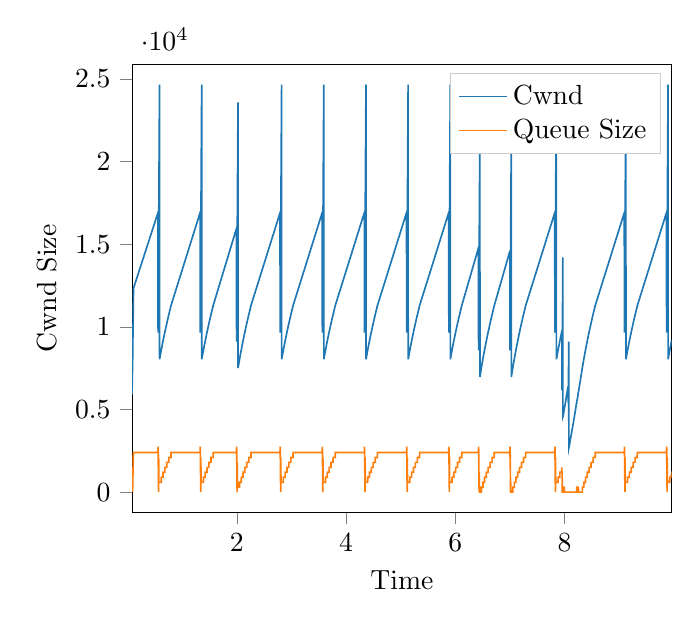
\begin{tikzpicture}

\definecolor{color0}{rgb}{0.12156862745098,0.466666666666667,0.705882352941177}
\definecolor{color1}{rgb}{1,0.498039215686275,0.0549019607843137}

\begin{axis}[
xlabel={Time},
ylabel={Cwnd Size},
xmin=0.0821184, xmax=9.96347,
ymin=-1232.8, ymax=25888.8,
tick align=outside,
tick pos=left,
x grid style={lightgray!92.026143790849673!black},
y grid style={lightgray!92.026143790849673!black},
legend cell align={left},
legend entries={{Cwnd},{Queue Size}},
legend style={draw=white!80.0!black}
]
\addlegendimage{no markers, color0}
\addlegendimage{no markers, color1}
\addplot [semithick, color0]
table {%
0.0821184 5896
0.0840064 6432
0.0858944 6968
0.0912608 7504
0.0931488 8040
0.0950368 8576
0.0969248 9112
0.0988128 9648
0.100701 10184
0.102589 10720
0.104477 11256
0.106365 11792
0.108253 12328
0.55382 16879
0.555708 16896
0.55854 9648
0.559484 10184
0.560428 10720
0.561372 11256
0.562316 11792
0.56326 12328
0.564204 12864
0.565148 13400
0.566092 13936
0.567036 14472
0.56798 15008
0.568924 15544
0.569868 16080
0.570812 16616
0.571756 17152
0.5727 17688
0.573644 18224
0.574588 18760
0.575532 19296
0.576476 19832
0.57742 20368
0.578364 20904
0.579308 21440
0.580252 21976
0.581196 22512
0.58214 23048
0.583084 23584
0.584028 24120
0.584972 24656
0.585916 8040
0.587804 8075
0.614236 8552
0.616124 8585
0.618012 8618
0.6199 8651
0.646332 9098
0.64822 9129
0.650108 9160
0.651996 9191
0.680316 9642
0.682204 9671
0.684092 9700
0.68598 9729
0.7143 10156
0.716188 10184
0.718076 10212
0.719964 10240
0.75206 10698
0.753948 10724
0.755836 10750
0.757724 10776
0.791708 11237
0.793596 11262
0.795484 11287
0.797372 11312
1.32601 16885
1.3279 16902
1.33073 9648
1.33168 10184
1.33262 10720
1.33356 11256
1.33451 11792
1.33545 12328
1.3364 12864
1.33734 13400
1.33828 13936
1.33923 14472
1.34017 15008
1.34112 15544
1.34206 16080
1.343 16616
1.34395 17152
1.34489 17688
1.34584 18224
1.34678 18760
1.34772 19296
1.34867 19832
1.34961 20368
1.35056 20904
1.3515 21440
1.35244 21976
1.35339 22512
1.35433 23048
1.35528 23584
1.35622 24120
1.35716 24656
1.35811 8040
1.36 8075
1.38643 8552
1.38832 8585
1.3902 8618
1.39209 8651
1.41852 9098
1.42041 9129
1.4223 9160
1.42419 9191
1.45251 9642
1.4544 9671
1.45628 9700
1.45817 9729
1.48649 10156
1.48838 10184
1.49027 10212
1.49216 10240
1.52425 10698
1.52614 10724
1.52803 10750
1.52992 10776
1.5639 11237
1.56579 11262
1.56768 11287
1.56956 11312
1.99059 15913
1.99247 15931
1.99625 9112
1.99719 9648
1.99814 10184
1.99908 10720
2.00003 11256
2.00097 11792
2.00191 12328
2.00286 12864
2.0038 13400
2.00475 13936
2.00569 14472
2.00663 15008
2.00758 15544
2.00852 16080
2.00947 16616
2.01041 17152
2.01135 17688
2.0123 18224
2.01324 18760
2.01419 19296
2.01513 19832
2.01607 20368
2.01702 20904
2.01796 21440
2.01891 21976
2.01985 22512
2.02079 23048
2.02174 23584
2.02268 7504
2.02457 7542
2.02646 7580
2.04911 8016
2.051 8051
2.05289 8086
2.05478 8121
2.07932 8563
2.08121 8596
2.0831 8629
2.08499 8662
2.11142 9108
2.11331 9139
2.11519 9170
2.11708 9201
2.14351 9623
2.1454 9652
2.14729 9681
2.14918 9710
2.17939 10165
2.18127 10193
2.18316 10221
2.18505 10249
2.21715 10707
2.21903 10733
2.22092 10759
2.22281 10785
2.25679 11246
2.25868 11271
2.26057 11296
2.26246 11321
2.78921 16873
2.7911 16890
2.79393 9648
2.79487 10184
2.79582 10720
2.79676 11256
2.79771 11792
2.79865 12328
2.79959 12864
2.80054 13400
2.80148 13936
2.80243 14472
2.80337 15008
2.80431 15544
2.80526 16080
2.8062 16616
2.80715 17152
2.80809 17688
2.80903 18224
2.80998 18760
2.81092 19296
2.81187 19832
2.81281 20368
2.81375 20904
2.8147 21440
2.81564 21976
2.81659 22512
2.81753 23048
2.81847 23584
2.81942 24120
2.82036 24656
2.82131 8040
2.82319 8075
2.84963 8552
2.85151 8585
2.8534 8618
2.85529 8651
2.88172 9098
2.88361 9129
2.8855 9160
2.88739 9191
2.91571 9642
2.91759 9671
2.91948 9700
2.92137 9729
2.94969 10156
2.95158 10184
2.95347 10212
2.95535 10240
2.98745 10698
2.98934 10724
2.99123 10750
2.99311 10776
3.0271 11237
3.02899 11262
3.03087 11287
3.03276 11312
3.5614 16885
3.56329 16902
3.56612 9648
3.56707 10184
3.56801 10720
3.56895 11256
3.5699 11792
3.57084 12328
3.57179 12864
3.57273 13400
3.57367 13936
3.57462 14472
3.57556 15008
3.57651 15544
3.57745 16080
3.57839 16616
3.57934 17152
3.58028 17688
3.58123 18224
3.58217 18760
3.58311 19296
3.58406 19832
3.585 20368
3.58595 20904
3.58689 21440
3.58783 21976
3.58878 22512
3.58972 23048
3.59067 23584
3.59161 24120
3.59255 24656
3.5935 8040
3.59539 8075
3.62182 8552
3.62371 8585
3.62559 8618
3.62748 8651
3.65391 9098
3.6558 9129
3.65769 9160
3.65958 9191
3.6879 9642
3.68978 9671
3.69167 9700
3.69356 9729
3.72188 10156
3.72377 10184
3.72566 10212
3.72754 10240
3.75964 10698
3.76153 10724
3.76342 10750
3.7653 10776
3.79929 11237
3.80118 11262
3.80306 11287
3.80495 11312
4.33359 16885
4.33548 16902
4.33831 9648
4.33926 10184
4.3402 10720
4.34114 11256
4.34209 11792
4.34303 12328
4.34398 12864
4.34492 13400
4.34586 13936
4.34681 14472
4.34775 15008
4.3487 15544
4.34964 16080
4.35058 16616
4.35153 17152
4.35247 17688
4.35342 18224
4.35436 18760
4.3553 19296
4.35625 19832
4.35719 20368
4.35814 20904
4.35908 21440
4.36002 21976
4.36097 22512
4.36191 23048
4.36286 23584
4.3638 24120
4.36474 24656
4.36569 8040
4.36758 8075
4.39401 8552
4.3959 8585
4.39778 8618
4.39967 8651
4.4261 9098
4.42799 9129
4.42988 9160
4.43177 9191
4.46009 9642
4.46198 9671
4.46386 9700
4.46575 9729
4.49407 10156
4.49596 10184
4.49785 10212
4.49974 10240
4.53183 10698
4.53372 10724
4.53561 10750
4.5375 10776
4.57148 11237
4.57337 11262
4.57526 11287
4.57714 11312
5.10578 16885
5.10767 16902
5.1105 9648
5.11145 10184
5.11239 10720
5.11334 11256
5.11428 11792
5.11522 12328
5.11617 12864
5.11711 13400
5.11806 13936
5.119 14472
5.11994 15008
5.12089 15544
5.12183 16080
5.12278 16616
5.12372 17152
5.12466 17688
5.12561 18224
5.12655 18760
5.1275 19296
5.12844 19832
5.12938 20368
5.13033 20904
5.13127 21440
5.13222 21976
5.13316 22512
5.1341 23048
5.13505 23584
5.13599 24120
5.13694 24656
5.13788 8040
5.13977 8075
5.1662 8552
5.16809 8585
5.16998 8618
5.17186 8651
5.1983 9098
5.20018 9129
5.20207 9160
5.20396 9191
5.23228 9642
5.23417 9671
5.23606 9700
5.23794 9729
5.26626 10156
5.26815 10184
5.27004 10212
5.27193 10240
5.30402 10698
5.30591 10724
5.3078 10750
5.30969 10776
5.34367 11237
5.34556 11262
5.34745 11287
5.34934 11312
5.87797 16885
5.87986 16902
5.88269 9648
5.88364 10184
5.88458 10720
5.88553 11256
5.88647 11792
5.88741 12328
5.88836 12864
5.8893 13400
5.89025 13936
5.89119 14472
5.89213 15008
5.89308 15544
5.89402 16080
5.89497 16616
5.89591 17152
5.89685 17688
5.8978 18224
5.89874 18760
5.89969 19296
5.90063 19832
5.90157 20368
5.90252 20904
5.90346 21440
5.90441 21976
5.90535 22512
5.90629 23048
5.90724 23584
5.90818 24120
5.90913 24656
5.91007 8040
5.91196 8075
5.93839 8552
5.94028 8585
5.94217 8618
5.94405 8651
5.97049 9098
5.97237 9129
5.97426 9160
5.97615 9191
6.00447 9642
6.00636 9671
6.00825 9700
6.01013 9729
6.03845 10156
6.04034 10184
6.04223 10212
6.04412 10240
6.07621 10698
6.0781 10724
6.07999 10750
6.08188 10776
6.11586 11237
6.11775 11262
6.11964 11287
6.12153 11312
6.42172 14741
6.42361 14760
6.42738 8576
6.42833 9112
6.42927 9648
6.43021 10184
6.43116 10720
6.4321 11256
6.43305 11792
6.43399 12328
6.43493 12864
6.43588 13400
6.43682 13936
6.43777 14472
6.43871 15008
6.43965 15544
6.4406 16080
6.44154 16616
6.44249 17152
6.44343 17688
6.44437 18224
6.44532 18760
6.44626 19296
6.44721 19832
6.44815 20368
6.44909 20904
6.45004 21440
6.45098 21976
6.45193 6968
6.45381 7009
6.4557 7049
6.47647 7480
6.47836 7518
6.48025 7556
6.48213 7594
6.50479 8030
6.50668 8065
6.50857 8100
6.51045 8135
6.53311 8544
6.535 8577
6.53689 8610
6.53877 8643
6.56521 9090
6.56709 9121
6.56898 9152
6.57087 9183
6.59919 9635
6.60108 9664
6.60297 9693
6.60485 9722
6.63506 10177
6.63695 10205
6.63884 10233
6.64073 10261
6.67282 10718
6.67471 10744
6.6766 10770
6.67849 10796
6.71058 11231
6.71247 11256
6.71436 11281
6.71625 11306
6.99567 14526
6.99756 14545
7.00039 14564
7.00322 8576
7.00417 9112
7.00511 9648
7.00605 10184
7.007 10720
7.00794 11256
7.00889 11792
7.00983 12328
7.01077 12864
7.01172 13400
7.01266 13936
7.01361 14472
7.01455 15008
7.01549 15544
7.01644 16080
7.01738 16616
7.01833 17152
7.01927 17688
7.02021 18224
7.02116 18760
7.0221 19296
7.02305 19832
7.02399 20368
7.02493 20904
7.02588 21440
7.02682 6968
7.02871 7009
7.05137 7480
7.05325 7518
7.05514 7556
7.05703 7594
7.07969 8030
7.08157 8065
7.08346 8100
7.08535 8135
7.10801 8544
7.10989 8577
7.11178 8610
7.11367 8643
7.1401 9090
7.14199 9121
7.14388 9152
7.14577 9183
7.17409 9635
7.17597 9664
7.17786 9693
7.17975 9722
7.20996 10177
7.21185 10205
7.21373 10233
7.21562 10261
7.24772 10718
7.24961 10744
7.25149 10770
7.25338 10796
7.28548 11231
7.28737 11256
7.28925 11281
7.29114 11306
7.81978 16880
7.82167 16897
7.8245 9648
7.82544 10184
7.82639 10720
7.82733 11256
7.82828 11792
7.82922 12328
7.83016 12864
7.83111 13400
7.83205 13936
7.833 14472
7.83394 15008
7.83488 15544
7.83583 16080
7.83677 16616
7.83772 17152
7.83866 17688
7.8396 18224
7.84055 18760
7.84149 19296
7.84244 19832
7.84338 20368
7.84432 20904
7.84527 21440
7.84621 21976
7.84716 22512
7.8481 23048
7.84904 23584
7.84999 24120
7.85093 24656
7.85188 8040
7.85376 8075
7.8802 8552
7.88208 8585
7.88397 8618
7.88586 8651
7.91229 9098
7.91418 9129
7.91607 9160
7.91796 9191
7.94628 9642
7.95005 9700
7.95288 9729
7.95572 6164
7.95666 6700
7.9576 7236
7.95855 7772
7.95949 8308
7.96044 8844
7.96138 9380
7.96232 9916
7.96327 10452
7.96421 10988
7.96516 11524
7.9661 12060
7.96704 12596
7.96799 13132
7.96893 13668
7.96988 14204
7.97082 4556
7.97713 4619
7.98279 4802
7.98911 4861
7.99099 4920
7.99477 5035
8.00108 5092
8.00297 5148
8.01211 5312
8.014 5366
8.02314 5524
8.02503 5576
8.03889 5876
8.04898 6067
8.0619 6342
8.06378 6387
8.07104 5360
8.07198 5896
8.07293 6432
8.07387 6968
8.07481 7504
8.07576 8040
8.0767 8576
8.07765 9112
8.08018 2680
8.08679 2787
8.16589 4263
8.17881 4525
8.19078 4771
8.20276 5006
8.21756 5338
8.22293 5391
8.22482 5444
8.22859 5548
8.23396 5599
8.23585 5650
8.24593 5848
8.24782 5897
8.24971 5945
8.25349 6040
8.25791 6087
8.2598 6134
8.27271 6407
8.28186 6582
8.32469 7474
8.32657 7512
8.32846 7550
8.33035 7588
8.35301 8024
8.35489 8059
8.35678 8094
8.35867 8129
8.38321 8571
8.3851 8604
8.38699 8637
8.38888 8670
8.41342 9085
8.41531 9116
8.4172 9147
8.41909 9178
8.44741 9630
8.44929 9659
8.45118 9688
8.45307 9717
8.48328 10172
8.48517 10200
8.48705 10228
8.48894 10256
8.52104 10714
8.52293 10740
8.52481 10766
8.5267 10792
8.56069 11252
8.56257 11277
8.56446 11302
8.56635 11327
9.0931 16878
9.09499 16895
9.09782 9648
9.09877 10184
9.09971 10720
9.10065 11256
9.1016 11792
9.10254 12328
9.10349 12864
9.10443 13400
9.10537 13936
9.10632 14472
9.10726 15008
9.10821 15544
9.10915 16080
9.11009 16616
9.11104 17152
9.11198 17688
9.11293 18224
9.11387 18760
9.11481 19296
9.11576 19832
9.1167 20368
9.11765 20904
9.11859 21440
9.11953 21976
9.12048 22512
9.12142 23048
9.12237 23584
9.12331 24120
9.12425 24656
9.1252 8040
9.12709 8075
9.15352 8552
9.15541 8585
9.15729 8618
9.15918 8651
9.18561 9098
9.1875 9129
9.18939 9160
9.19128 9191
9.2196 9642
9.22149 9671
9.22337 9700
9.22526 9729
9.25358 10156
9.25547 10184
9.25736 10212
9.25924 10240
9.29134 10698
9.29323 10724
9.29512 10750
9.297 10776
9.33099 11237
9.33288 11262
9.33476 11287
9.33665 11312
9.86529 16885
9.86718 16902
9.87001 9648
9.87096 10184
9.8719 10720
9.87284 11256
9.87379 11792
9.87473 12328
9.87568 12864
9.87662 13400
9.87756 13936
9.87851 14472
9.87945 15008
9.8804 15544
9.88134 16080
9.88228 16616
9.88323 17152
9.88417 17688
9.88512 18224
9.88606 18760
9.887 19296
9.88795 19832
9.88889 20368
9.88984 20904
9.89078 21440
9.89172 21976
9.89267 22512
9.89361 23048
9.89456 23584
9.8955 24120
9.89644 24656
9.89739 8040
9.89928 8075
9.92571 8552
9.9276 8585
9.92948 8618
9.93137 8651
9.9578 9098
9.95969 9129
9.96158 9160
9.96347 9191
};
\addplot [semithick, color1]
table {%
0.0821184 300
0.0840064 600
0.0858944 900
0.0912608 0
0.0931488 300
0.0950368 600
0.0969248 900
0.0988128 1200
0.100701 1500
0.102589 1800
0.104477 2100
0.106365 2400
0.108253 2400
0.55382 2400
0.555708 2400
0.55854 2700
0.559484 2700
0.560428 2400
0.561372 2100
0.562316 1800
0.56326 1500
0.564204 1200
0.565148 900
0.566092 600
0.567036 300
0.56798 0
0.568924 2100
0.569868 1800
0.570812 1500
0.571756 1200
0.5727 900
0.573644 600
0.574588 600
0.575532 600
0.576476 600
0.57742 600
0.578364 600
0.579308 600
0.580252 600
0.581196 600
0.58214 600
0.583084 600
0.584028 600
0.584972 600
0.585916 600
0.587804 600
0.614236 600
0.616124 600
0.618012 900
0.6199 900
0.646332 900
0.64822 900
0.650108 1200
0.651996 1200
0.680316 1200
0.682204 1200
0.684092 1500
0.68598 1500
0.7143 1500
0.716188 1500
0.718076 1800
0.719964 1800
0.75206 1800
0.753948 1800
0.755836 2100
0.757724 2100
0.791708 2100
0.793596 2100
0.795484 2400
0.797372 2400
1.32601 2400
1.3279 2400
1.33073 2700
1.33168 2700
1.33262 2400
1.33356 2100
1.33451 1800
1.33545 1500
1.3364 1200
1.33734 900
1.33828 600
1.33923 300
1.34017 0
1.34112 2100
1.34206 1800
1.343 1500
1.34395 1200
1.34489 900
1.34584 600
1.34678 600
1.34772 600
1.34867 600
1.34961 600
1.35056 600
1.3515 600
1.35244 600
1.35339 600
1.35433 600
1.35528 600
1.35622 600
1.35716 600
1.35811 600
1.36 600
1.38643 600
1.38832 600
1.3902 900
1.39209 900
1.41852 900
1.42041 900
1.4223 1200
1.42419 1200
1.45251 1200
1.4544 1200
1.45628 1500
1.45817 1500
1.48649 1500
1.48838 1500
1.49027 1800
1.49216 1800
1.52425 1800
1.52614 1800
1.52803 2100
1.52992 2100
1.5639 2100
1.56579 2100
1.56768 2400
1.56956 2400
1.99059 2400
1.99247 2400
1.99625 2700
1.99719 2700
1.99814 2400
1.99908 2100
2.00003 1800
2.00097 1500
2.00191 1200
2.00286 900
2.0038 600
2.00475 300
2.00569 0
2.00663 1800
2.00758 1500
2.00852 1200
2.00947 900
2.01041 600
2.01135 600
2.0123 600
2.01324 600
2.01419 600
2.01513 600
2.01607 600
2.01702 600
2.01796 600
2.01891 600
2.01985 600
2.02079 600
2.02174 600
2.02268 600
2.02457 300
2.02646 300
2.04911 300
2.051 300
2.05289 600
2.05478 600
2.07932 600
2.08121 600
2.0831 900
2.08499 900
2.11142 900
2.11331 900
2.11519 1200
2.11708 1200
2.14351 1200
2.1454 1200
2.14729 1500
2.14918 1500
2.17939 1500
2.18127 1500
2.18316 1800
2.18505 1800
2.21715 1800
2.21903 1800
2.22092 2100
2.22281 2100
2.25679 2100
2.25868 2100
2.26057 2400
2.26246 2400
2.78921 2400
2.7911 2400
2.79393 2700
2.79487 2700
2.79582 2400
2.79676 2100
2.79771 1800
2.79865 1500
2.79959 1200
2.80054 900
2.80148 600
2.80243 300
2.80337 0
2.80431 2100
2.80526 1800
2.8062 1500
2.80715 1200
2.80809 900
2.80903 600
2.80998 600
2.81092 600
2.81187 600
2.81281 600
2.81375 600
2.8147 600
2.81564 600
2.81659 600
2.81753 600
2.81847 600
2.81942 600
2.82036 600
2.82131 600
2.82319 600
2.84963 600
2.85151 600
2.8534 900
2.85529 900
2.88172 900
2.88361 900
2.8855 1200
2.88739 1200
2.91571 1200
2.91759 1200
2.91948 1500
2.92137 1500
2.94969 1500
2.95158 1500
2.95347 1800
2.95535 1800
2.98745 1800
2.98934 1800
2.99123 2100
2.99311 2100
3.0271 2100
3.02899 2100
3.03087 2400
3.03276 2400
3.5614 2400
3.56329 2400
3.56612 2700
3.56707 2700
3.56801 2400
3.56895 2100
3.5699 1800
3.57084 1500
3.57179 1200
3.57273 900
3.57367 600
3.57462 300
3.57556 0
3.57651 2100
3.57745 1800
3.57839 1500
3.57934 1200
3.58028 900
3.58123 600
3.58217 600
3.58311 600
3.58406 600
3.585 600
3.58595 600
3.58689 600
3.58783 600
3.58878 600
3.58972 600
3.59067 600
3.59161 600
3.59255 600
3.5935 600
3.59539 600
3.62182 600
3.62371 600
3.62559 900
3.62748 900
3.65391 900
3.6558 900
3.65769 1200
3.65958 1200
3.6879 1200
3.68978 1200
3.69167 1500
3.69356 1500
3.72188 1500
3.72377 1500
3.72566 1800
3.72754 1800
3.75964 1800
3.76153 1800
3.76342 2100
3.7653 2100
3.79929 2100
3.80118 2100
3.80306 2400
3.80495 2400
4.33359 2400
4.33548 2400
4.33831 2700
4.33926 2700
4.3402 2400
4.34114 2100
4.34209 1800
4.34303 1500
4.34398 1200
4.34492 900
4.34586 600
4.34681 300
4.34775 0
4.3487 2100
4.34964 1800
4.35058 1500
4.35153 1200
4.35247 900
4.35342 600
4.35436 600
4.3553 600
4.35625 600
4.35719 600
4.35814 600
4.35908 600
4.36002 600
4.36097 600
4.36191 600
4.36286 600
4.3638 600
4.36474 600
4.36569 600
4.36758 600
4.39401 600
4.3959 600
4.39778 900
4.39967 900
4.4261 900
4.42799 900
4.42988 1200
4.43177 1200
4.46009 1200
4.46198 1200
4.46386 1500
4.46575 1500
4.49407 1500
4.49596 1500
4.49785 1800
4.49974 1800
4.53183 1800
4.53372 1800
4.53561 2100
4.5375 2100
4.57148 2100
4.57337 2100
4.57526 2400
4.57714 2400
5.10578 2400
5.10767 2400
5.1105 2700
5.11145 2700
5.11239 2400
5.11334 2100
5.11428 1800
5.11522 1500
5.11617 1200
5.11711 900
5.11806 600
5.119 300
5.11994 0
5.12089 2100
5.12183 1800
5.12278 1500
5.12372 1200
5.12466 900
5.12561 600
5.12655 600
5.1275 600
5.12844 600
5.12938 600
5.13033 600
5.13127 600
5.13222 600
5.13316 600
5.1341 600
5.13505 600
5.13599 600
5.13694 600
5.13788 600
5.13977 600
5.1662 600
5.16809 600
5.16998 900
5.17186 900
5.1983 900
5.20018 900
5.20207 1200
5.20396 1200
5.23228 1200
5.23417 1200
5.23606 1500
5.23794 1500
5.26626 1500
5.26815 1500
5.27004 1800
5.27193 1800
5.30402 1800
5.30591 1800
5.3078 2100
5.30969 2100
5.34367 2100
5.34556 2100
5.34745 2400
5.34934 2400
5.87797 2400
5.87986 2400
5.88269 2700
5.88364 2700
5.88458 2400
5.88553 2100
5.88647 1800
5.88741 1500
5.88836 1200
5.8893 900
5.89025 600
5.89119 300
5.89213 0
5.89308 2100
5.89402 1800
5.89497 1500
5.89591 1200
5.89685 900
5.8978 600
5.89874 600
5.89969 600
5.90063 600
5.90157 600
5.90252 600
5.90346 600
5.90441 600
5.90535 600
5.90629 600
5.90724 600
5.90818 600
5.90913 600
5.91007 600
5.91196 600
5.93839 600
5.94028 600
5.94217 900
5.94405 900
5.97049 900
5.97237 900
5.97426 1200
5.97615 1200
6.00447 1200
6.00636 1200
6.00825 1500
6.01013 1500
6.03845 1500
6.04034 1500
6.04223 1800
6.04412 1800
6.07621 1800
6.0781 1800
6.07999 2100
6.08188 2100
6.11586 2100
6.11775 2100
6.11964 2400
6.12153 2400
6.42172 2400
6.42361 2400
6.42738 2700
6.42833 2700
6.42927 2400
6.43021 2100
6.43116 1800
6.4321 1500
6.43305 1200
6.43399 900
6.43493 600
6.43588 300
6.43682 0
6.43777 1200
6.43871 900
6.43965 600
6.4406 300
6.44154 300
6.44249 300
6.44343 300
6.44437 300
6.44532 300
6.44626 300
6.44721 300
6.44815 300
6.44909 300
6.45004 300
6.45098 300
6.45193 300
6.45381 0
6.4557 0
6.47647 0
6.47836 0
6.48025 300
6.48213 300
6.50479 300
6.50668 300
6.50857 600
6.51045 600
6.53311 600
6.535 600
6.53689 900
6.53877 900
6.56521 900
6.56709 900
6.56898 1200
6.57087 1200
6.59919 1200
6.60108 1200
6.60297 1500
6.60485 1500
6.63506 1500
6.63695 1500
6.63884 1800
6.64073 1800
6.67282 1800
6.67471 1800
6.6766 2100
6.67849 2100
6.71058 2100
6.71247 2100
6.71436 2400
6.71625 2400
6.99567 2400
6.99756 2400
7.00039 2100
7.00322 2700
7.00417 2700
7.00511 2400
7.00605 2100
7.007 1800
7.00794 1500
7.00889 1200
7.00983 900
7.01077 600
7.01172 300
7.01266 0
7.01361 900
7.01455 600
7.01549 300
7.01644 0
7.01738 0
7.01833 0
7.01927 0
7.02021 0
7.02116 0
7.0221 0
7.02305 0
7.02399 0
7.02493 0
7.02588 0
7.02682 0
7.02871 0
7.05137 0
7.05325 0
7.05514 300
7.05703 300
7.07969 300
7.08157 300
7.08346 600
7.08535 600
7.10801 600
7.10989 600
7.11178 900
7.11367 900
7.1401 900
7.14199 900
7.14388 1200
7.14577 1200
7.17409 1200
7.17597 1200
7.17786 1500
7.17975 1500
7.20996 1500
7.21185 1500
7.21373 1800
7.21562 1800
7.24772 1800
7.24961 1800
7.25149 2100
7.25338 2100
7.28548 2100
7.28737 2100
7.28925 2400
7.29114 2400
7.81978 2400
7.82167 2400
7.8245 2700
7.82544 2700
7.82639 2400
7.82733 2100
7.82828 1800
7.82922 1500
7.83016 1200
7.83111 900
7.83205 600
7.833 300
7.83394 0
7.83488 2100
7.83583 1800
7.83677 1500
7.83772 1200
7.83866 900
7.8396 600
7.84055 600
7.84149 600
7.84244 600
7.84338 600
7.84432 600
7.84527 600
7.84621 600
7.84716 600
7.8481 600
7.84904 600
7.84999 600
7.85093 600
7.85188 600
7.85376 600
7.8802 600
7.88208 600
7.88397 900
7.88586 900
7.91229 900
7.91418 900
7.91607 1200
7.91796 1200
7.94628 1200
7.95005 1500
7.95288 1200
7.95572 1200
7.95666 1200
7.9576 900
7.95855 600
7.95949 300
7.96044 0
7.96138 0
7.96232 0
7.96327 0
7.96421 0
7.96516 0
7.9661 0
7.96704 0
7.96799 0
7.96893 0
7.96988 0
7.97082 0
7.97713 0
7.98279 0
7.98911 0
7.99099 300
7.99477 300
8.00108 0
8.00297 0
8.01211 0
8.014 0
8.02314 0
8.02503 0
8.03889 0
8.04898 0
8.0619 0
8.06378 0
8.07104 0
8.07198 0
8.07293 0
8.07387 0
8.07481 0
8.07576 0
8.0767 0
8.07765 0
8.08018 0
8.08679 0
8.16589 0
8.17881 0
8.19078 0
8.20276 0
8.21756 0
8.22293 0
8.22482 300
8.22859 300
8.23396 0
8.23585 0
8.24593 0
8.24782 0
8.24971 300
8.25349 300
8.25791 0
8.2598 0
8.27271 0
8.28186 0
8.32469 0
8.32657 0
8.32846 300
8.33035 300
8.35301 300
8.35489 300
8.35678 600
8.35867 600
8.38321 600
8.3851 600
8.38699 900
8.38888 900
8.41342 900
8.41531 900
8.4172 1200
8.41909 1200
8.44741 1200
8.44929 1200
8.45118 1500
8.45307 1500
8.48328 1500
8.48517 1500
8.48705 1800
8.48894 1800
8.52104 1800
8.52293 1800
8.52481 2100
8.5267 2100
8.56069 2100
8.56257 2100
8.56446 2400
8.56635 2400
9.0931 2400
9.09499 2400
9.09782 2700
9.09877 2700
9.09971 2400
9.10065 2100
9.1016 1800
9.10254 1500
9.10349 1200
9.10443 900
9.10537 600
9.10632 300
9.10726 0
9.10821 2100
9.10915 1800
9.11009 1500
9.11104 1200
9.11198 900
9.11293 600
9.11387 600
9.11481 600
9.11576 600
9.1167 600
9.11765 600
9.11859 600
9.11953 600
9.12048 600
9.12142 600
9.12237 600
9.12331 600
9.12425 600
9.1252 600
9.12709 600
9.15352 600
9.15541 600
9.15729 900
9.15918 900
9.18561 900
9.1875 900
9.18939 1200
9.19128 1200
9.2196 1200
9.22149 1200
9.22337 1500
9.22526 1500
9.25358 1500
9.25547 1500
9.25736 1800
9.25924 1800
9.29134 1800
9.29323 1800
9.29512 2100
9.297 2100
9.33099 2100
9.33288 2100
9.33476 2400
9.33665 2400
9.86529 2400
9.86718 2400
9.87001 2700
9.87096 2700
9.8719 2400
9.87284 2100
9.87379 1800
9.87473 1500
9.87568 1200
9.87662 900
9.87756 600
9.87851 300
9.87945 0
9.8804 2100
9.88134 1800
9.88228 1500
9.88323 1200
9.88417 900
9.88512 600
9.88606 600
9.887 600
9.88795 600
9.88889 600
9.88984 600
9.89078 600
9.89172 600
9.89267 600
9.89361 600
9.89456 600
9.8955 600
9.89644 600
9.89739 600
9.89928 600
9.92571 600
9.9276 600
9.92948 900
9.93137 900
9.9578 900
9.95969 900
9.96158 1200
9.96347 1200
};
\end{axis}

\end{tikzpicture}% This file was created by matplotlib2tikz v0.6.13.
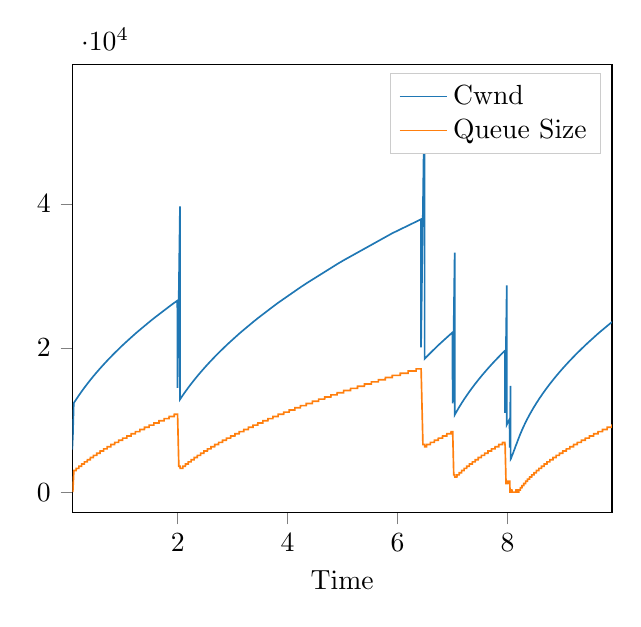
\begin{tikzpicture}

\definecolor{color0}{rgb}{0.12156862745098,0.466666666666667,0.705882352941177}
\definecolor{color1}{rgb}{1,0.498039215686275,0.0549019607843137}

\begin{axis}[
xlabel={Time},
xmin=0.0821184, xmax=9.9015,
ymin=-2827.4, ymax=59375.4,
tick align=outside,
tick pos=left,
x grid style={lightgray!92.026143790849673!black},
y grid style={lightgray!92.026143790849673!black},
legend cell align={left},
legend entries={{Cwnd},{Queue Size}},
legend style={draw=white!80.0!black}
]
\addlegendimage{no markers, color0}
\addlegendimage{no markers, color1}
\addplot [semithick, color0]
table {%
0.0821184 5896
0.0840064 6432
0.0858944 6968
0.0912608 7504
0.0931488 8040
0.0950368 8576
0.0969248 9112
0.0988128 9648
0.100701 10184
0.102589 10720
0.104477 11256
0.106365 11792
0.108253 12328
0.108253 12351
0.110141 12374
0.112029 12397
0.149789 12842
0.151677 12864
0.153565 12886
0.155453 12908
0.198877 13398
0.200765 13419
0.202653 13440
0.204541 13461
0.247965 13932
0.249853 13952
0.251741 13972
0.253629 13992
0.298941 14467
0.300829 14486
0.302717 14505
0.304605 14524
0.351805 14999
0.353693 15018
0.355581 15037
0.357469 15056
0.406556 15528
0.408444 15546
0.410332 15564
0.41222 15582
0.463196 16063
0.465084 16080
0.466972 16097
0.46886 16114
0.523612 16607
0.5255 16624
0.527388 16641
0.529276 16658
0.584028 17137
0.585916 17153
0.587804 17169
0.589692 17185
0.64822 17681
0.650108 17697
0.651996 17713
0.653884 17729
0.712412 18209
0.7143 18224
0.716188 18239
0.718076 18254
0.78038 18749
0.782268 18764
0.784156 18779
0.786044 18794
0.850236 19294
0.852124 19308
0.854012 19322
0.8559 19336
0.92198 19826
0.923868 19840
0.925756 19854
0.927644 19868
0.993724 20358
0.995612 20372
0.9975 20386
0.999388 20400
1.07113 20903
1.07302 20916
1.07491 20929
1.0768 20942
1.14854 21436
1.15043 21449
1.15232 21462
1.1542 21475
1.22595 21969
1.22784 21982
1.22972 21995
1.23161 22008
1.30902 22508
1.31091 22520
1.3128 22532
1.31468 22544
1.39209 23036
1.39398 23048
1.39587 23060
1.39776 23072
1.47705 23576
1.47894 23588
1.48083 23600
1.48272 23612
1.5639 24113
1.56579 24124
1.56768 24135
1.56956 24146
1.65641 24652
1.6583 24663
1.66019 24674
1.66208 24685
1.74892 25191
1.75081 25202
1.7527 25213
1.75459 25224
1.83955 25719
1.84143 25730
1.84332 25741
1.84521 25752
1.93395 26256
1.93583 26266
1.93772 26276
1.93961 26286
1.99059 26556
1.99247 26566
1.99625 14472
1.99719 15008
1.99814 15544
1.99908 16080
2.00003 16616
2.00097 17152
2.00191 17688
2.00286 18224
2.0038 18760
2.00475 19296
2.00569 19832
2.00663 20368
2.00758 20904
2.00852 21440
2.00947 21976
2.01041 22512
2.01135 23048
2.0123 23584
2.01324 24120
2.01419 24656
2.01513 25192
2.01607 25728
2.01702 26264
2.01796 26800
2.01891 27336
2.01985 27872
2.02079 28408
2.02174 28944
2.02268 29480
2.02363 30016
2.02457 30552
2.02551 31088
2.02646 31624
2.0274 32160
2.02835 32696
2.02929 33232
2.03023 33768
2.03118 34304
2.03212 34840
2.03307 35376
2.03401 35912
2.03495 36448
2.0359 36984
2.03684 37520
2.03779 38056
2.03873 38592
2.03967 39128
2.04062 39664
2.04156 12864
2.04345 12886
2.04534 12908
2.08876 13398
2.09065 13419
2.09254 13440
2.09443 13461
2.13785 13932
2.13974 13952
2.14163 13972
2.14351 13992
2.18883 14467
2.19071 14486
2.1926 14505
2.19449 14524
2.24169 14999
2.24358 15018
2.24547 15037
2.24735 15056
2.29644 15528
2.29833 15546
2.30022 15564
2.30211 15582
2.35308 16063
2.35497 16080
2.35686 16097
2.35875 16114
2.4135 16607
2.41539 16624
2.41727 16641
2.41916 16658
2.47391 17137
2.4758 17153
2.47769 17169
2.47958 17185
2.53811 17681
2.53999 17697
2.54188 17713
2.54377 17729
2.6023 18209
2.60419 18224
2.60607 18239
2.60796 18254
2.67027 18749
2.67215 18764
2.67404 18779
2.67593 18794
2.74012 19294
2.74201 19308
2.7439 19322
2.74579 19336
2.81187 19826
2.81375 19840
2.81564 19854
2.81753 19868
2.88361 20358
2.8855 20372
2.88739 20386
2.88927 20400
2.96102 20903
2.96291 20916
2.96479 20929
2.96668 20942
3.03843 21436
3.04031 21449
3.0422 21462
3.04409 21475
3.11583 21969
3.11772 21982
3.11961 21995
3.1215 22008
3.19891 22508
3.20079 22520
3.20268 22532
3.20457 22544
3.28198 23036
3.28387 23048
3.28575 23060
3.28764 23072
3.36694 23576
3.36883 23588
3.37071 23600
3.3726 23612
3.45379 24113
3.45567 24124
3.45756 24135
3.45945 24146
3.5463 24652
3.54819 24663
3.55007 24674
3.55196 24685
3.63881 25191
3.6407 25202
3.64259 25213
3.64447 25224
3.72943 25719
3.73132 25730
3.73321 25741
3.7351 25752
3.82383 26256
3.82572 26266
3.82761 26276
3.8295 26286
3.92578 26796
3.92767 26806
3.92956 26816
3.93145 26826
4.02585 27326
4.02774 27336
4.02962 27346
4.03151 27356
4.1278 27866
4.12969 27876
4.13158 27886
4.13346 27896
4.22975 28406
4.23164 28416
4.23353 28426
4.23542 28436
4.33548 28943
4.33737 28952
4.33926 28961
4.34114 28970
4.44687 29474
4.44876 29483
4.45065 29492
4.45254 29501
4.56015 30014
4.56204 30023
4.56393 30032
4.56582 30041
4.67154 30545
4.67343 30554
4.67532 30563
4.67721 30572
4.78482 31085
4.78671 31094
4.7886 31103
4.79049 31112
4.89622 31616
4.8981 31625
4.89999 31634
4.90188 31643
5.01516 32154
5.01705 32162
5.01894 32170
5.02082 32178
5.14166 32690
5.14354 32698
5.14543 32706
5.14732 32714
5.26815 33226
5.27004 33234
5.27193 33242
5.27382 33250
5.39465 33762
5.39654 33770
5.39842 33778
5.40031 33786
5.52114 34298
5.52303 34306
5.52492 34314
5.52681 34322
5.64764 34834
5.64953 34842
5.65141 34850
5.6533 34858
5.77413 35370
5.77602 35378
5.77791 35386
5.7798 35394
5.90063 35906
5.90252 35914
5.90441 35921
5.90629 35928
6.04601 36446
6.04789 36453
6.04978 36460
6.05167 36467
6.18949 36978
6.19138 36985
6.19327 36992
6.19516 36999
6.33487 37517
6.33676 37524
6.33865 37531
6.34053 37538
6.42172 37839
6.42361 37846
6.42738 20100
6.42833 20636
6.42927 21172
6.43021 21708
6.43116 22244
6.4321 22780
6.43305 23316
6.43399 23852
6.43493 24388
6.43588 24924
6.43682 25460
6.43777 25996
6.43871 26532
6.43965 27068
6.4406 27604
6.44154 28140
6.44249 28676
6.44343 29212
6.44437 29748
6.44532 30284
6.44626 30820
6.44721 31356
6.44815 31892
6.44909 32428
6.45004 32964
6.45098 33500
6.45193 34036
6.45287 34572
6.45381 35108
6.45476 35644
6.4557 36180
6.45665 36716
6.45759 37252
6.45853 37788
6.45948 38324
6.46042 38860
6.46137 39396
6.46231 39932
6.46325 40468
6.4642 41004
6.46514 41540
6.46609 42076
6.46703 42612
6.46797 43148
6.46892 43684
6.46986 44220
6.47081 44756
6.47175 45292
6.47269 45828
6.47364 46364
6.47458 46900
6.47553 47436
6.47647 47972
6.47741 48508
6.47836 49044
6.4793 49580
6.48025 50116
6.48119 50652
6.48213 51188
6.48308 51724
6.48402 52260
6.48497 52796
6.48591 53332
6.48685 53868
6.4878 54404
6.48874 54940
6.48969 55476
6.49063 56012
6.49157 56548
6.49252 18492
6.49441 18507
6.49629 18522
6.52461 18747
6.5265 18762
6.52839 18777
6.53028 18792
6.59447 19293
6.59636 19307
6.59825 19321
6.60013 19335
6.66621 19825
6.6681 19839
6.66999 19853
6.67188 19867
6.73796 20357
6.73985 20371
6.74173 20385
6.74362 20399
6.81537 20902
6.81725 20915
6.81914 20928
6.82103 20941
6.89277 21435
6.89466 21448
6.89655 21461
6.89844 21474
6.97018 21968
6.97207 21981
6.97396 21994
6.97585 22007
6.99661 22147
6.9985 22159
7.00228 12328
7.00322 12864
7.00417 13400
7.00511 13936
7.00605 14472
7.007 15008
7.00794 15544
7.00889 16080
7.00983 16616
7.01077 17152
7.01172 17688
7.01266 18224
7.01361 18760
7.01455 19296
7.01549 19832
7.01644 20368
7.01738 20904
7.01833 21440
7.01927 21976
7.02021 22512
7.02116 23048
7.0221 23584
7.02305 24120
7.02399 24656
7.02493 25192
7.02588 25728
7.02682 26264
7.02777 26800
7.02871 27336
7.02965 27872
7.0306 28408
7.03154 28944
7.03249 29480
7.03343 30016
7.03437 30552
7.03532 31088
7.03626 31624
7.03721 32160
7.03815 32696
7.03909 33232
7.04004 10720
7.04193 10746
7.04381 10772
7.0778 11233
7.07969 11258
7.08157 11283
7.08346 11308
7.11933 11772
7.12122 11796
7.12311 11820
7.125 11844
7.16276 12310
7.16465 12333
7.16653 12356
7.16842 12379
7.20807 12846
7.20996 12868
7.21185 12890
7.21373 12912
7.25527 13381
7.25716 13402
7.25905 13423
7.26093 13444
7.30436 13916
7.30625 13936
7.30813 13956
7.31002 13976
7.35722 14471
7.35911 14490
7.361 14509
7.36289 14528
7.41009 15003
7.41197 15022
7.41386 15041
7.41575 15060
7.46484 15532
7.46672 15550
7.46861 15568
7.4705 15586
7.52148 16066
7.52336 16083
7.52525 16100
7.52714 16117
7.58189 16610
7.58378 16627
7.58567 16644
7.58756 16661
7.64231 17140
7.6442 17156
7.64608 17172
7.64797 17188
7.7065 17684
7.70839 17700
7.71028 17716
7.71216 17732
7.77069 18212
7.77258 18227
7.77447 18242
7.77636 18257
7.83866 18752
7.84055 18767
7.84244 18782
7.84432 18797
7.90663 19283
7.90852 19297
7.9104 19311
7.91229 19325
7.94816 19591
7.95005 19605
7.95288 19619
7.95572 10988
7.95666 11524
7.9576 12060
7.95855 12596
7.95949 13132
7.96044 13668
7.96138 14204
7.96232 14740
7.96327 15276
7.96421 15812
7.96516 16348
7.9661 16884
7.96704 17420
7.96799 17956
7.96893 18492
7.96988 19028
7.97082 19564
7.97176 20100
7.97271 20636
7.97365 21172
7.9746 21708
7.97554 22244
7.97648 22780
7.97743 23316
7.97837 23852
7.97932 24388
7.98026 24924
7.9812 25460
7.98215 25996
7.98309 26532
7.98404 27068
7.98498 27604
7.98592 28140
7.98687 28676
7.98781 9380
7.9897 9410
8.00292 9619
8.0048 9648
8.00669 9677
8.00858 9706
8.03501 10105
8.0369 10133
8.04068 6164
8.04162 6700
8.04256 7236
8.04351 7772
8.04445 8308
8.0454 8844
8.04634 9380
8.04728 9916
8.04823 10452
8.04917 10988
8.05012 11524
8.05106 12060
8.052 12596
8.05295 13132
8.05389 13668
8.05484 14204
8.05578 14740
8.05672 4556
8.06209 4619
8.06775 4802
8.07407 4861
8.07595 4920
8.07973 5035
8.08604 5092
8.08793 5148
8.09707 5312
8.09896 5366
8.1081 5524
8.10999 5576
8.12385 5876
8.13394 6067
8.15063 6431
8.15411 6475
8.156 6519
8.15789 6563
8.15977 6606
8.16166 6649
8.16514 6692
8.16703 6734
8.17711 6942
8.179 6983
8.18089 7024
8.18278 7064
8.18467 7104
8.18655 7144
8.18909 7184
8.19098 7223
8.20419 7493
8.20608 7531
8.20797 7569
8.20986 7606
8.23063 8007
8.23251 8042
8.2344 8077
8.23629 8112
8.26083 8554
8.26272 8587
8.26461 8620
8.2665 8653
8.29293 9100
8.29482 9131
8.29671 9162
8.29859 9193
8.32691 9644
8.3288 9673
8.33069 9702
8.33258 9731
8.3609 10158
8.36278 10186
8.36467 10214
8.36656 10242
8.39866 10700
8.40054 10726
8.40243 10752
8.40432 10778
8.4383 11239
8.44019 11264
8.44208 11289
8.44397 11314
8.47984 11778
8.48173 11802
8.48362 11826
8.4855 11850
8.52326 12316
8.52515 12339
8.52704 12362
8.52893 12385
8.56858 12852
8.57046 12874
8.57235 12896
8.57424 12918
8.61578 13387
8.61766 13408
8.61955 13429
8.62144 13450
8.66486 13921
8.66675 13941
8.66864 13961
8.67053 13981
8.71584 14457
8.71773 14476
8.71962 14495
8.7215 14514
8.7687 14989
8.77059 15008
8.77248 15027
8.77437 15046
8.82534 15536
8.82723 15554
8.82912 15572
8.83101 15590
8.88198 16070
8.88387 16087
8.88576 16104
8.88765 16121
8.9424 16614
8.94429 16631
8.94618 16648
8.94806 16665
9.00282 17143
9.0047 17159
9.00659 17175
9.00848 17191
9.06701 17687
9.0689 17703
9.07078 17719
9.07267 17735
9.1312 18214
9.13309 18229
9.13498 18244
9.13686 18259
9.19917 18754
9.20106 18769
9.20294 18784
9.20483 18799
9.26714 19285
9.26902 19299
9.27091 19313
9.2728 19327
9.34077 19831
9.34266 19845
9.34454 19859
9.34643 19873
9.41251 20363
9.4144 20377
9.41629 20391
9.41818 20405
9.48803 20895
9.48992 20908
9.49181 20921
9.4937 20934
9.56544 21428
9.56733 21441
9.56922 21454
9.5711 21467
9.64474 21974
9.64662 21987
9.64851 22000
9.6504 22013
9.72592 22500
9.72781 22512
9.7297 22524
9.73158 22536
9.81088 23040
9.81277 23052
9.81466 23064
9.81654 23076
9.89584 23580
9.89773 23592
9.89962 23604
9.9015 23616
};
\addplot [semithick, color1]
table {%
0.0821184 300
0.0840064 600
0.0858944 900
0.0912608 0
0.0931488 300
0.0950368 600
0.0969248 900
0.0988128 1200
0.100701 1500
0.102589 1800
0.104477 2100
0.106365 2400
0.108253 2700
0.108253 2700
0.110141 3000
0.112029 3000
0.149789 3000
0.151677 3000
0.153565 3300
0.155453 3300
0.198877 3300
0.200765 3300
0.202653 3600
0.204541 3600
0.247965 3600
0.249853 3600
0.251741 3900
0.253629 3900
0.298941 3900
0.300829 3900
0.302717 4200
0.304605 4200
0.351805 4200
0.353693 4200
0.355581 4500
0.357469 4500
0.406556 4500
0.408444 4500
0.410332 4800
0.41222 4800
0.463196 4800
0.465084 4800
0.466972 5100
0.46886 5100
0.523612 5100
0.5255 5100
0.527388 5400
0.529276 5400
0.584028 5400
0.585916 5400
0.587804 5700
0.589692 5700
0.64822 5700
0.650108 5700
0.651996 6000
0.653884 6000
0.712412 6000
0.7143 6000
0.716188 6300
0.718076 6300
0.78038 6300
0.782268 6300
0.784156 6600
0.786044 6600
0.850236 6600
0.852124 6600
0.854012 6900
0.8559 6900
0.92198 6900
0.923868 6900
0.925756 7200
0.927644 7200
0.993724 7200
0.995612 7200
0.9975 7500
0.999388 7500
1.07113 7500
1.07302 7500
1.07491 7800
1.0768 7800
1.14854 7800
1.15043 7800
1.15232 8100
1.1542 8100
1.22595 8100
1.22784 8100
1.22972 8400
1.23161 8400
1.30902 8400
1.31091 8400
1.3128 8700
1.31468 8700
1.39209 8700
1.39398 8700
1.39587 9000
1.39776 9000
1.47705 9000
1.47894 9000
1.48083 9300
1.48272 9300
1.5639 9300
1.56579 9300
1.56768 9600
1.56956 9600
1.65641 9600
1.6583 9600
1.66019 9900
1.66208 9900
1.74892 9900
1.75081 9900
1.7527 10200
1.75459 10200
1.83955 10200
1.84143 10200
1.84332 10500
1.84521 10500
1.93395 10500
1.93583 10500
1.93772 10800
1.93961 10800
1.99059 10800
1.99247 10800
1.99625 10800
1.99719 10800
1.99814 10500
1.99908 10200
2.00003 9900
2.00097 9600
2.00191 9300
2.00286 9000
2.0038 8700
2.00475 8400
2.00569 8100
2.00663 7800
2.00758 7500
2.00852 7200
2.00947 6900
2.01041 6600
2.01135 6300
2.0123 6000
2.01324 5700
2.01419 5400
2.01513 5100
2.01607 4800
2.01702 4500
2.01796 4200
2.01891 3900
2.01985 3600
2.02079 3600
2.02174 3600
2.02268 3600
2.02363 3600
2.02457 3600
2.02551 3600
2.02646 3600
2.0274 3600
2.02835 3600
2.02929 3600
2.03023 3600
2.03118 3600
2.03212 3600
2.03307 3600
2.03401 3600
2.03495 3600
2.0359 3600
2.03684 3600
2.03779 3600
2.03873 3600
2.03967 3600
2.04062 3600
2.04156 3600
2.04345 3300
2.04534 3300
2.08876 3300
2.09065 3300
2.09254 3600
2.09443 3600
2.13785 3600
2.13974 3600
2.14163 3900
2.14351 3900
2.18883 3900
2.19071 3900
2.1926 4200
2.19449 4200
2.24169 4200
2.24358 4200
2.24547 4500
2.24735 4500
2.29644 4500
2.29833 4500
2.30022 4800
2.30211 4800
2.35308 4800
2.35497 4800
2.35686 5100
2.35875 5100
2.4135 5100
2.41539 5100
2.41727 5400
2.41916 5400
2.47391 5400
2.4758 5400
2.47769 5700
2.47958 5700
2.53811 5700
2.53999 5700
2.54188 6000
2.54377 6000
2.6023 6000
2.60419 6000
2.60607 6300
2.60796 6300
2.67027 6300
2.67215 6300
2.67404 6600
2.67593 6600
2.74012 6600
2.74201 6600
2.7439 6900
2.74579 6900
2.81187 6900
2.81375 6900
2.81564 7200
2.81753 7200
2.88361 7200
2.8855 7200
2.88739 7500
2.88927 7500
2.96102 7500
2.96291 7500
2.96479 7800
2.96668 7800
3.03843 7800
3.04031 7800
3.0422 8100
3.04409 8100
3.11583 8100
3.11772 8100
3.11961 8400
3.1215 8400
3.19891 8400
3.20079 8400
3.20268 8700
3.20457 8700
3.28198 8700
3.28387 8700
3.28575 9000
3.28764 9000
3.36694 9000
3.36883 9000
3.37071 9300
3.3726 9300
3.45379 9300
3.45567 9300
3.45756 9600
3.45945 9600
3.5463 9600
3.54819 9600
3.55007 9900
3.55196 9900
3.63881 9900
3.6407 9900
3.64259 10200
3.64447 10200
3.72943 10200
3.73132 10200
3.73321 10500
3.7351 10500
3.82383 10500
3.82572 10500
3.82761 10800
3.8295 10800
3.92578 10800
3.92767 10800
3.92956 11100
3.93145 11100
4.02585 11100
4.02774 11100
4.02962 11400
4.03151 11400
4.1278 11400
4.12969 11400
4.13158 11700
4.13346 11700
4.22975 11700
4.23164 11700
4.23353 12000
4.23542 12000
4.33548 12000
4.33737 12000
4.33926 12300
4.34114 12300
4.44687 12300
4.44876 12300
4.45065 12600
4.45254 12600
4.56015 12600
4.56204 12600
4.56393 12900
4.56582 12900
4.67154 12900
4.67343 12900
4.67532 13200
4.67721 13200
4.78482 13200
4.78671 13200
4.7886 13500
4.79049 13500
4.89622 13500
4.8981 13500
4.89999 13800
4.90188 13800
5.01516 13800
5.01705 13800
5.01894 14100
5.02082 14100
5.14166 14100
5.14354 14100
5.14543 14400
5.14732 14400
5.26815 14400
5.27004 14400
5.27193 14700
5.27382 14700
5.39465 14700
5.39654 14700
5.39842 15000
5.40031 15000
5.52114 15000
5.52303 15000
5.52492 15300
5.52681 15300
5.64764 15300
5.64953 15300
5.65141 15600
5.6533 15600
5.77413 15600
5.77602 15600
5.77791 15900
5.7798 15900
5.90063 15900
5.90252 15900
5.90441 16200
5.90629 16200
6.04601 16200
6.04789 16200
6.04978 16500
6.05167 16500
6.18949 16500
6.19138 16500
6.19327 16800
6.19516 16800
6.33487 16800
6.33676 16800
6.33865 17100
6.34053 17100
6.42172 17100
6.42361 17100
6.42738 17100
6.42833 17100
6.42927 16800
6.43021 16500
6.43116 16200
6.4321 15900
6.43305 15600
6.43399 15300
6.43493 15000
6.43588 14700
6.43682 14400
6.43777 14100
6.43871 13800
6.43965 13500
6.4406 13200
6.44154 12900
6.44249 12600
6.44343 12300
6.44437 12000
6.44532 11700
6.44626 11400
6.44721 11100
6.44815 10800
6.44909 10500
6.45004 10200
6.45098 9900
6.45193 9600
6.45287 9300
6.45381 9000
6.45476 8700
6.4557 8400
6.45665 8100
6.45759 7800
6.45853 7500
6.45948 7200
6.46042 6900
6.46137 6600
6.46231 6600
6.46325 6600
6.4642 6600
6.46514 6600
6.46609 6600
6.46703 6600
6.46797 6600
6.46892 6600
6.46986 6600
6.47081 6600
6.47175 6600
6.47269 6600
6.47364 6600
6.47458 6600
6.47553 6600
6.47647 6600
6.47741 6600
6.47836 6600
6.4793 6600
6.48025 6600
6.48119 6600
6.48213 6600
6.48308 6600
6.48402 6600
6.48497 6600
6.48591 6600
6.48685 6600
6.4878 6600
6.48874 6600
6.48969 6600
6.49063 6600
6.49157 6600
6.49252 6600
6.49441 6300
6.49629 6300
6.52461 6300
6.5265 6300
6.52839 6600
6.53028 6600
6.59447 6600
6.59636 6600
6.59825 6900
6.60013 6900
6.66621 6900
6.6681 6900
6.66999 7200
6.67188 7200
6.73796 7200
6.73985 7200
6.74173 7500
6.74362 7500
6.81537 7500
6.81725 7500
6.81914 7800
6.82103 7800
6.89277 7800
6.89466 7800
6.89655 8100
6.89844 8100
6.97018 8100
6.97207 8100
6.97396 8400
6.97585 8400
6.99661 8400
6.9985 8400
7.00228 8400
7.00322 8400
7.00417 8100
7.00511 7800
7.00605 7500
7.007 7200
7.00794 6900
7.00889 6600
7.00983 6300
7.01077 6000
7.01172 5700
7.01266 5400
7.01361 5100
7.01455 4800
7.01549 4500
7.01644 4200
7.01738 3900
7.01833 3600
7.01927 3300
7.02021 3000
7.02116 2700
7.0221 2400
7.02305 2400
7.02399 2400
7.02493 2400
7.02588 2400
7.02682 2400
7.02777 2400
7.02871 2400
7.02965 2400
7.0306 2400
7.03154 2400
7.03249 2400
7.03343 2400
7.03437 2400
7.03532 2400
7.03626 2400
7.03721 2400
7.03815 2400
7.03909 2400
7.04004 2400
7.04193 2100
7.04381 2100
7.0778 2100
7.07969 2100
7.08157 2400
7.08346 2400
7.11933 2400
7.12122 2400
7.12311 2700
7.125 2700
7.16276 2700
7.16465 2700
7.16653 3000
7.16842 3000
7.20807 3000
7.20996 3000
7.21185 3300
7.21373 3300
7.25527 3300
7.25716 3300
7.25905 3600
7.26093 3600
7.30436 3600
7.30625 3600
7.30813 3900
7.31002 3900
7.35722 3900
7.35911 3900
7.361 4200
7.36289 4200
7.41009 4200
7.41197 4200
7.41386 4500
7.41575 4500
7.46484 4500
7.46672 4500
7.46861 4800
7.4705 4800
7.52148 4800
7.52336 4800
7.52525 5100
7.52714 5100
7.58189 5100
7.58378 5100
7.58567 5400
7.58756 5400
7.64231 5400
7.6442 5400
7.64608 5700
7.64797 5700
7.7065 5700
7.70839 5700
7.71028 6000
7.71216 6000
7.77069 6000
7.77258 6000
7.77447 6300
7.77636 6300
7.83866 6300
7.84055 6300
7.84244 6600
7.84432 6600
7.90663 6600
7.90852 6600
7.9104 6900
7.91229 6900
7.94816 6900
7.95005 6900
7.95288 6600
7.95572 6600
7.95666 6600
7.9576 6300
7.95855 6000
7.95949 5700
7.96044 5400
7.96138 5100
7.96232 4800
7.96327 4500
7.96421 4200
7.96516 3900
7.9661 3600
7.96704 3300
7.96799 3000
7.96893 2700
7.96988 2400
7.97082 2100
7.97176 1800
7.97271 1500
7.97365 1200
7.9746 1200
7.97554 1200
7.97648 1200
7.97743 1200
7.97837 1200
7.97932 1200
7.98026 1200
7.9812 1200
7.98215 1200
7.98309 1200
7.98404 1200
7.98498 1200
7.98592 1200
7.98687 1200
7.98781 1200
7.9897 1200
8.00292 1200
8.0048 1200
8.00669 1500
8.00858 1500
8.03501 1500
8.0369 1500
8.04068 1500
8.04162 1500
8.04256 1200
8.04351 900
8.04445 600
8.0454 300
8.04634 0
8.04728 0
8.04823 0
8.04917 0
8.05012 0
8.05106 0
8.052 0
8.05295 0
8.05389 0
8.05484 0
8.05578 0
8.05672 0
8.06209 0
8.06775 0
8.07407 0
8.07595 300
8.07973 300
8.08604 0
8.08793 0
8.09707 0
8.09896 0
8.1081 0
8.10999 0
8.12385 0
8.13394 0
8.15063 0
8.15411 0
8.156 300
8.15789 300
8.15977 300
8.16166 300
8.16514 0
8.16703 0
8.17711 0
8.179 0
8.18089 300
8.18278 300
8.18467 300
8.18655 300
8.18909 0
8.19098 0
8.20419 0
8.20608 0
8.20797 300
8.20986 300
8.23063 300
8.23251 300
8.2344 600
8.23629 600
8.26083 600
8.26272 600
8.26461 900
8.2665 900
8.29293 900
8.29482 900
8.29671 1200
8.29859 1200
8.32691 1200
8.3288 1200
8.33069 1500
8.33258 1500
8.3609 1500
8.36278 1500
8.36467 1800
8.36656 1800
8.39866 1800
8.40054 1800
8.40243 2100
8.40432 2100
8.4383 2100
8.44019 2100
8.44208 2400
8.44397 2400
8.47984 2400
8.48173 2400
8.48362 2700
8.4855 2700
8.52326 2700
8.52515 2700
8.52704 3000
8.52893 3000
8.56858 3000
8.57046 3000
8.57235 3300
8.57424 3300
8.61578 3300
8.61766 3300
8.61955 3600
8.62144 3600
8.66486 3600
8.66675 3600
8.66864 3900
8.67053 3900
8.71584 3900
8.71773 3900
8.71962 4200
8.7215 4200
8.7687 4200
8.77059 4200
8.77248 4500
8.77437 4500
8.82534 4500
8.82723 4500
8.82912 4800
8.83101 4800
8.88198 4800
8.88387 4800
8.88576 5100
8.88765 5100
8.9424 5100
8.94429 5100
8.94618 5400
8.94806 5400
9.00282 5400
9.0047 5400
9.00659 5700
9.00848 5700
9.06701 5700
9.0689 5700
9.07078 6000
9.07267 6000
9.1312 6000
9.13309 6000
9.13498 6300
9.13686 6300
9.19917 6300
9.20106 6300
9.20294 6600
9.20483 6600
9.26714 6600
9.26902 6600
9.27091 6900
9.2728 6900
9.34077 6900
9.34266 6900
9.34454 7200
9.34643 7200
9.41251 7200
9.4144 7200
9.41629 7500
9.41818 7500
9.48803 7500
9.48992 7500
9.49181 7800
9.4937 7800
9.56544 7800
9.56733 7800
9.56922 8100
9.5711 8100
9.64474 8100
9.64662 8100
9.64851 8400
9.6504 8400
9.72592 8400
9.72781 8400
9.7297 8700
9.73158 8700
9.81088 8700
9.81277 8700
9.81466 9000
9.81654 9000
9.89584 9000
9.89773 9000
9.89962 9300
9.9015 9300
};
\end{axis}

\end{tikzpicture}\\

It can be seen that the throughput is slightly higher with a larger queue. This is because while a larger queue helps keep more packets with the device, hence increasing cwnd, the queueing delay also increases due to a bigger queue. This balances out and the throughput increases only by a small amount. An ideal maximum queue size would be around the number of packets that get filled up at the end of the congestion avoidance phase. This way, there will not be a big queue, but the queue would not be filled completely either.
\end{enumerate}

  \begin{center}
  Created using \LaTeX \ with Overleaf and TexStudio with MiKTeX
  \end{center}
  \end{document}